\documentclass[a4paper,10pt]{scrreprt}
\usepackage[utf8]{inputenc}
\usepackage{graphicx}
\usepackage{mathtools}
\usepackage{amsfonts}
\usepackage{amsmath}
\usepackage{amssymb}
\usepackage{amsthm}
\usepackage{siunitx}
\usepackage{gnuplottex}
\usepackage{fullpage}
\usepackage{wrapfig}
\usepackage{hyperref}
\usepackage{url}
\usepackage{float}
\usepackage{caption}
\usepackage{subcaption}
\usepackage{verbatim}
\usepackage{tabularx}

%\setcounter{tocdepth}{4}

%\usepackage{pxfonts} 

\linespread{1.2}

\DeclareMathOperator*{\argmax}{arg\,max}
\DeclareMathOperator*{\argmin}{arg\,min}

\newcommand*{\diffd}{\mathrm{d}}

\newcommand{\matr}[1]{\mathbf{#1}}
\newcommand{\hommatr}[1]{\hat{\mathbf{#1}}}
\newcommand{\transpose}[1]{#1^\intercal}
\newcommand{\homvec}[1]{\vec{\hat{#1}}}
\newcommand{\colvecT}[1]{\left[#1\right]^\intercal}
\newcommand{\rowvec}[1]{\left[#1\right]}
\newcommand{\coreq}{\hat{=}}
\newcommand{\area}[1]{\mathcal{A}(#1)}



%\mathtoolsset{showonlyrefs=true}

\begin{document}

\title{Registration and fusion of large scale three-dimensional models}
\author{Tim Lenertz}
\date{\today}
\maketitle

\tableofcontents

\chapter{Introduction}

\chapter{State of the Art}

\section{3D Scanning}
The general goal of a 3D scanning project is to create a digital model of a physical three-dimensional object. Different methodologies exist for all sizes and types of objects. This section will give an overview of the process of 3D scanning, including the technology involved in obtaining 3D data, the operations that are performed to process it, and the final results that a 3D scanning project aims to obtain.

Possibly the most simple case is to scan the surface of a single, solid object. Examples include artefacts such as the commonly used \emph{Stanford Bunny}, models of teeth or bones for manufacturing of prosthesis, small archeological artifacts, etc. The object is idealised mathematically as a single closed two-dimensional surface embedded in three-dimensional space.

To scan an object 3D scanners and photogrammetry is typically used.  Laser scanners emit light and detect the reflections from the object, in order to record a set of three-dimensional coordinates of points that lie on the object's surfaces. For smaller objects contact scanners also exist which physically probe the object. Photogrammetry consists of taking multiple photographic pictures of the object, and algorithmically recovering depth information by comparing photos from different camera poses. The scanning system can be set up such that the object and/or the scanners of cameras are rotated such that the entire object is covered.

For larger of more complex objects, or objects embedded in a more complex environment, it becomes harder to delimit the targeted content, and to filter it out from the raw scans. This is for instance the case for buildings \cite{Kers2006}, archeological sites \cite{Web1} \cite{Kein2011} \cite{Grus2012} or rock formations. It may be desirable to have a higher resolution for specific parts of the scene. In these cases, data will be collected using a combination of laser scanning and photogrammetry, where the scanner is kept at a fixed position relative to the object. The result is a \emph{range image} or \emph{depth map}, which is a projected two-dimensional image of the object from a given view point where each pixel contains depth information.

Post-processing of the 3D scans consists in filtering the raw data and combining range images and photographs from different view points, in order to obtain a 3D model of the entire object. This resulting 3D model is an approximation of the real object's surfaces, typically in the form of a set of unconnected points (\emph{point cloud}), or of a \emph{mesh} of vertices forming triangular faces. In some applications, such as in architecture or in retro-engineering, the goal is to obtain a CAD model, in which shapes such as planes or cylinders, or more complex objects are identified. 

In other contexts, specifically in medical imaging, the goal is not to scan surfaces, but the whole inside of an object. Here techniques such as \emph{computed tomography} and \emph{magnetic resonance imaging} are used, and a volumetric model of the object in the form of \emph{voxel data} is produced. A \emph{voxel} is the three-dimensional equivalent of a \emph{pixel}.

Other applications of laser scanning include for example meteorology, where backscatter in the atmosphere is measured, forestry, where airborne laser scanning is used to obtain a height-map of a terrain with multiple layers representing the ground and treetops, the scanning of astronomical objects, robotics \cite{Bibe2003} and autonomous vehicles, and more.

This paper focusses on the problem of registering different scans of parts of the same object, especially in the case where the scans are of different resolutions. The scanned object is modeled to be an ensemble of continuous surfaces, and the point clouds a discrete set of points from those surfaces. 


\subsection{Point cloud}
In the context of this paper, data obtained from 3D scanning is recorded in the form of a \emph{point cloud}. An unorganized point cloud is defined as a set $P = \{ (x_i, y_i, z_i) \}$ of \emph{points}, each of which have spatial coordinates set in a coordinate system specific for this scan. Each point can be attributed with additional information, such as an RGB color, a temperature, or the normal vector of the surface at that point. Laser scanners usually collect an intensity value that records the strength of the reflected light beam from that point, and possibly a confidence value for the correctness of the point.

Point clouds hold no information about the connectivity of the points that form a surface of the object. Points that are considered to be samples of a surface are called \emph{inliers}. Each inlier has a certain \emph{error}, as a result of the limited precision of the scanner, and due to properties of the material. The error can be defined as the point's offset from the actual surface. Points that do form part of the object surface are called \emph{outliers}. They may be the result of unwanted content that got scanned along with the targeted object, or any other \emph{noise} data that appears during the processing pipeline.

Representing real objects using point clouds can be considered a two-fold modeling of physical reality: First it is assumed that the object is a set of continuous, solid surfaces. This disregards material properties such as surface reflectance and transparency, fine-scale texture of the surface and the resulting effects on light reflection, small scale motions of the object. Within this model point attributes such as a surface normal vector and a color are defined, and points are classified as inliers or outliers. Then this surfaces model gets represented by means of a sparse set of points, which introduces additional considerations such as the dispersion, density and uncertainty of the points.

This notion is vague, and can be inappropriate when the real object is too complex to be modeled that way. For example for brick wall covered with climbing plants, scanned at low resolution, which are possible in motion during the scan, there is not enough information available in the scan to represent the surfaces of the individual leaves. When instead considering the wall as one plane, the vegetation gets represented as an error value in subsequent processing.


\subsection{Range image}
Additional information can be contained in the ordering of the points in the set. Laser scanners probe their field of view by sending out rays in different directions in a well-defined order. Typically the elevation and azimuth angles are gradually incremented and reset in a line-by-line manner, forming a two-dimensional grid in the field of view. Knowing the width and height of this grid, the ordered point cloud corresponds to a \emph{range image}: Each pixel in the range image corresponds to either a point $p_i \in P$, or an invalid point $\epsilon$, in case when no reflected ray was received in the direction it was pointing at. The range image can be described as the function $r : \mathbb{N}^2 \rightarrow P \cup \{ \epsilon \}$. In the case of a stationary laser scanner, the pixel coordinates would map to the azimuth and elevation angles of the point in spherical coordinates. The exact nature of this mapping is determined by the scanner, and it not necessarily a linear mapping. However it is such that a small difference in the pixel coordinates corresponds to a small difference in azimuth and elevation, which can for example be used to find neighbouring points efficiently. Creating a picture where each pixel $(x, y)$ gets the color attributed to the point $r(x, y)$ (or a background color when $r(x, y) = \epsilon$), gives a photographic view of the scan. An example is shown on figures \ref{fig:hdv_033_color} (point color) and \ref{fig:hdv_033_range} (distances from point to camera), taken from the ``Hôtel de Ville'' scans. For this scanner the mapping to pixel coordinates is not a linear mapping of the spherical coordinates, as can be seen by the curvatures of corners.

\begin{figure}[p]
\center
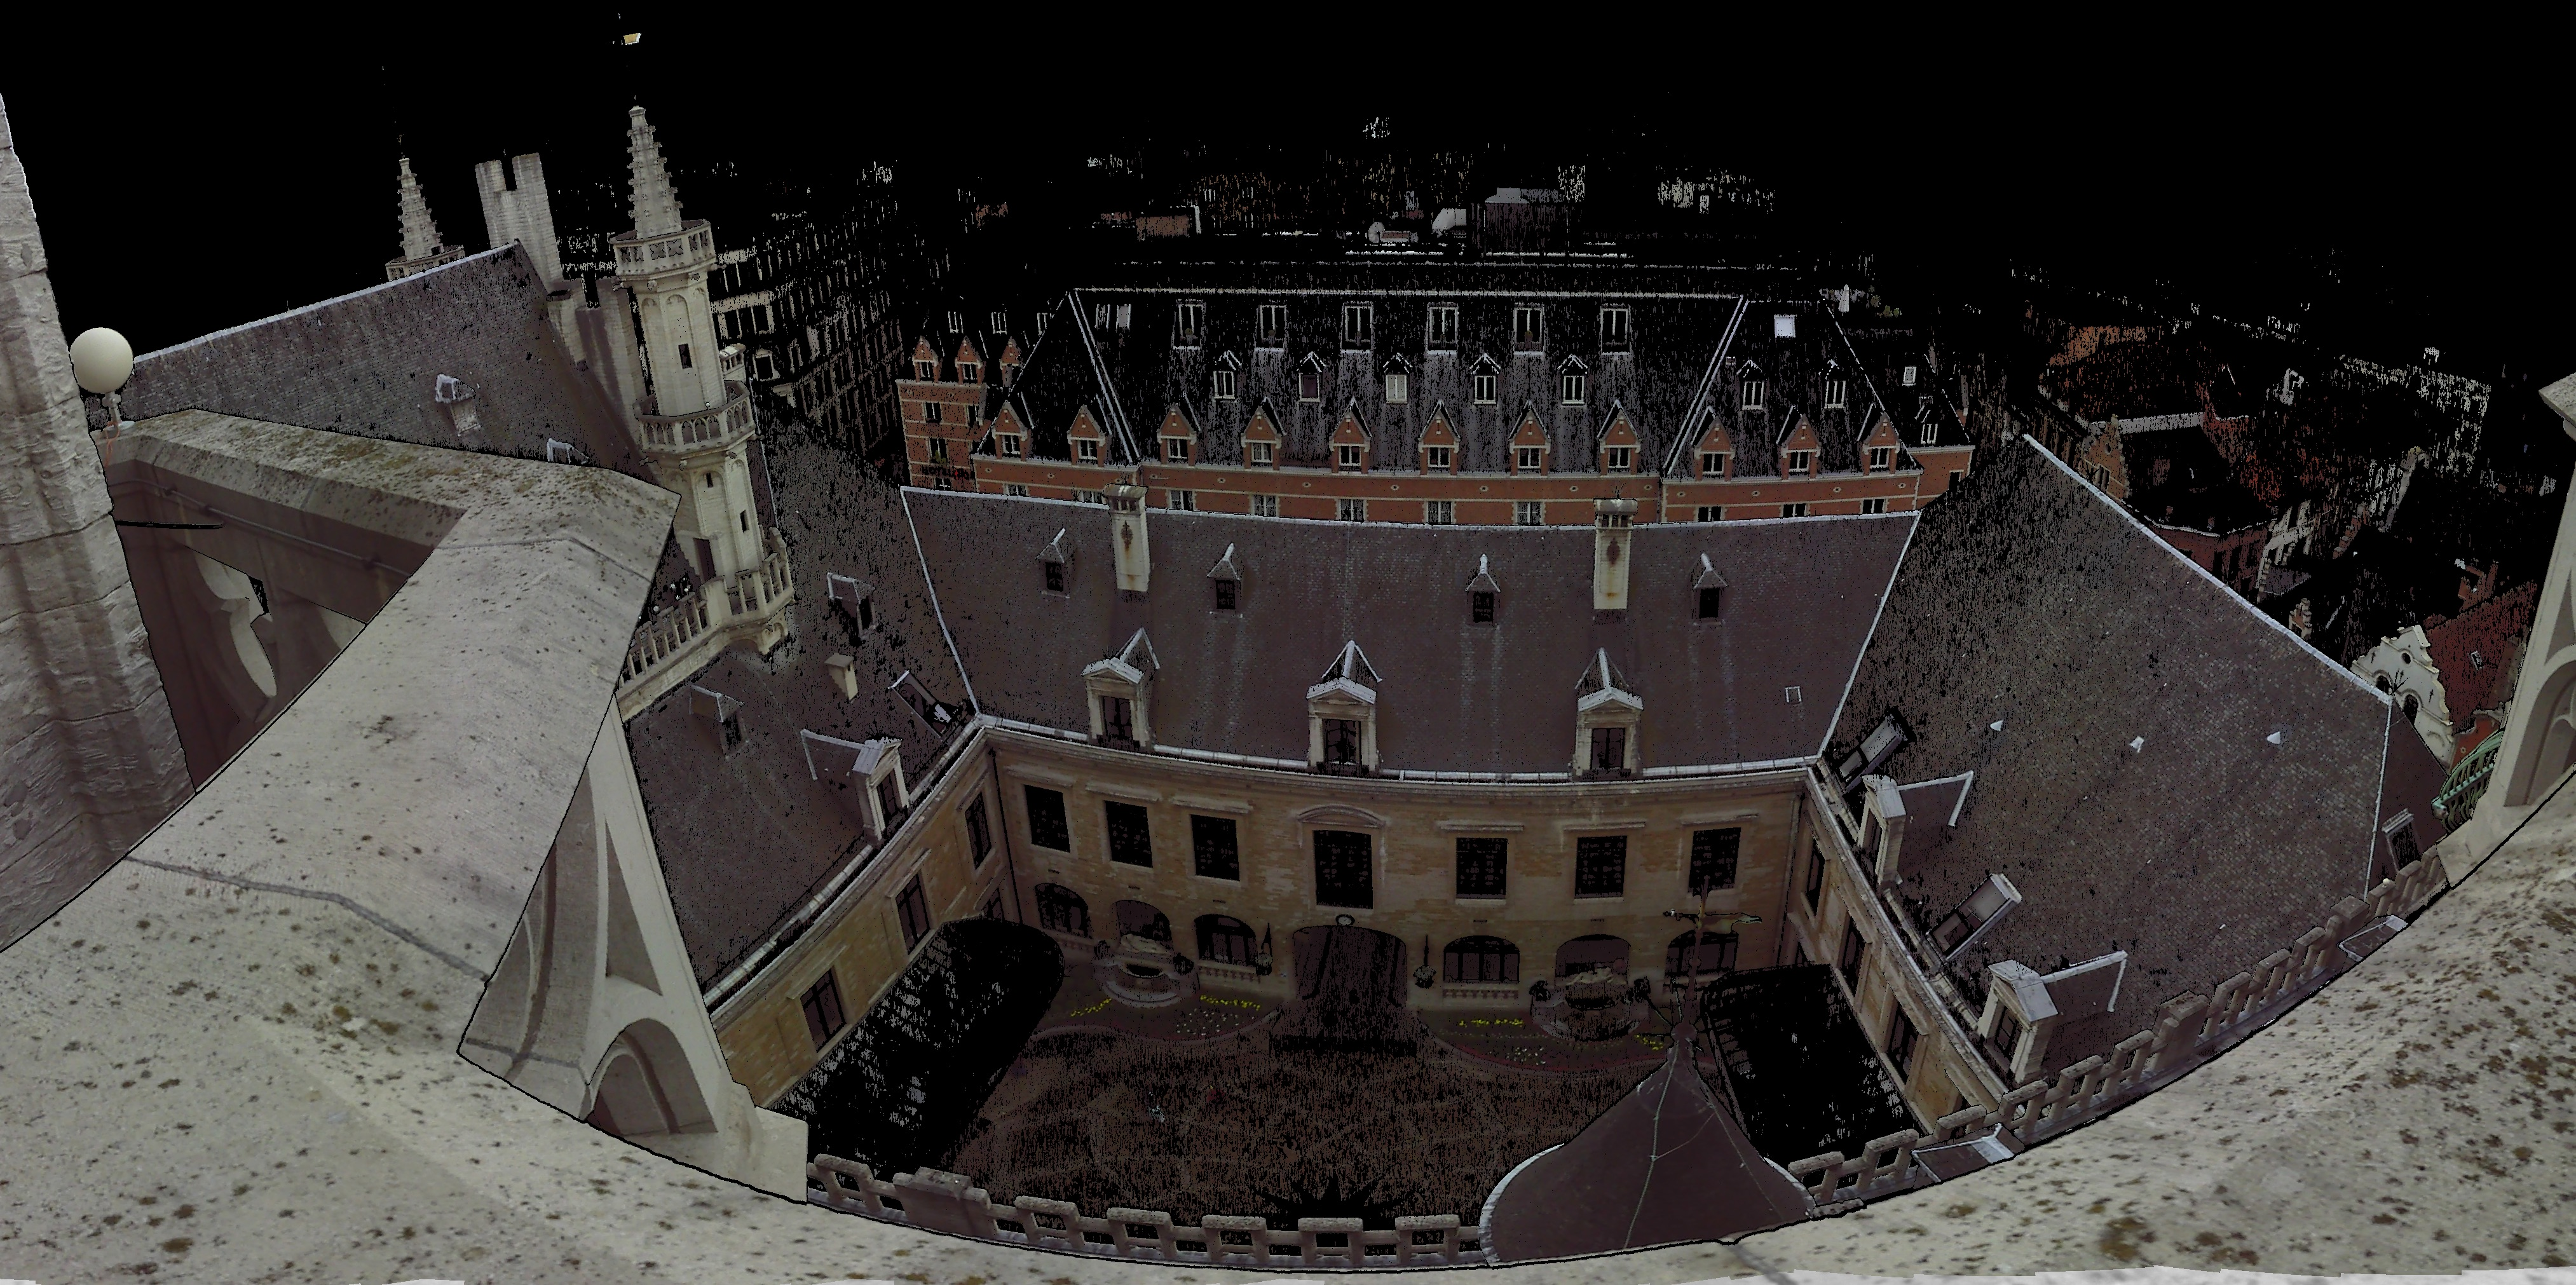
\includegraphics[width=.8\textwidth]{fig/hdv_033_color.jpg}
\label{fig:hdv_033_color}
\caption{Color view of range image}
\end{figure}

\begin{figure}[p]
\center
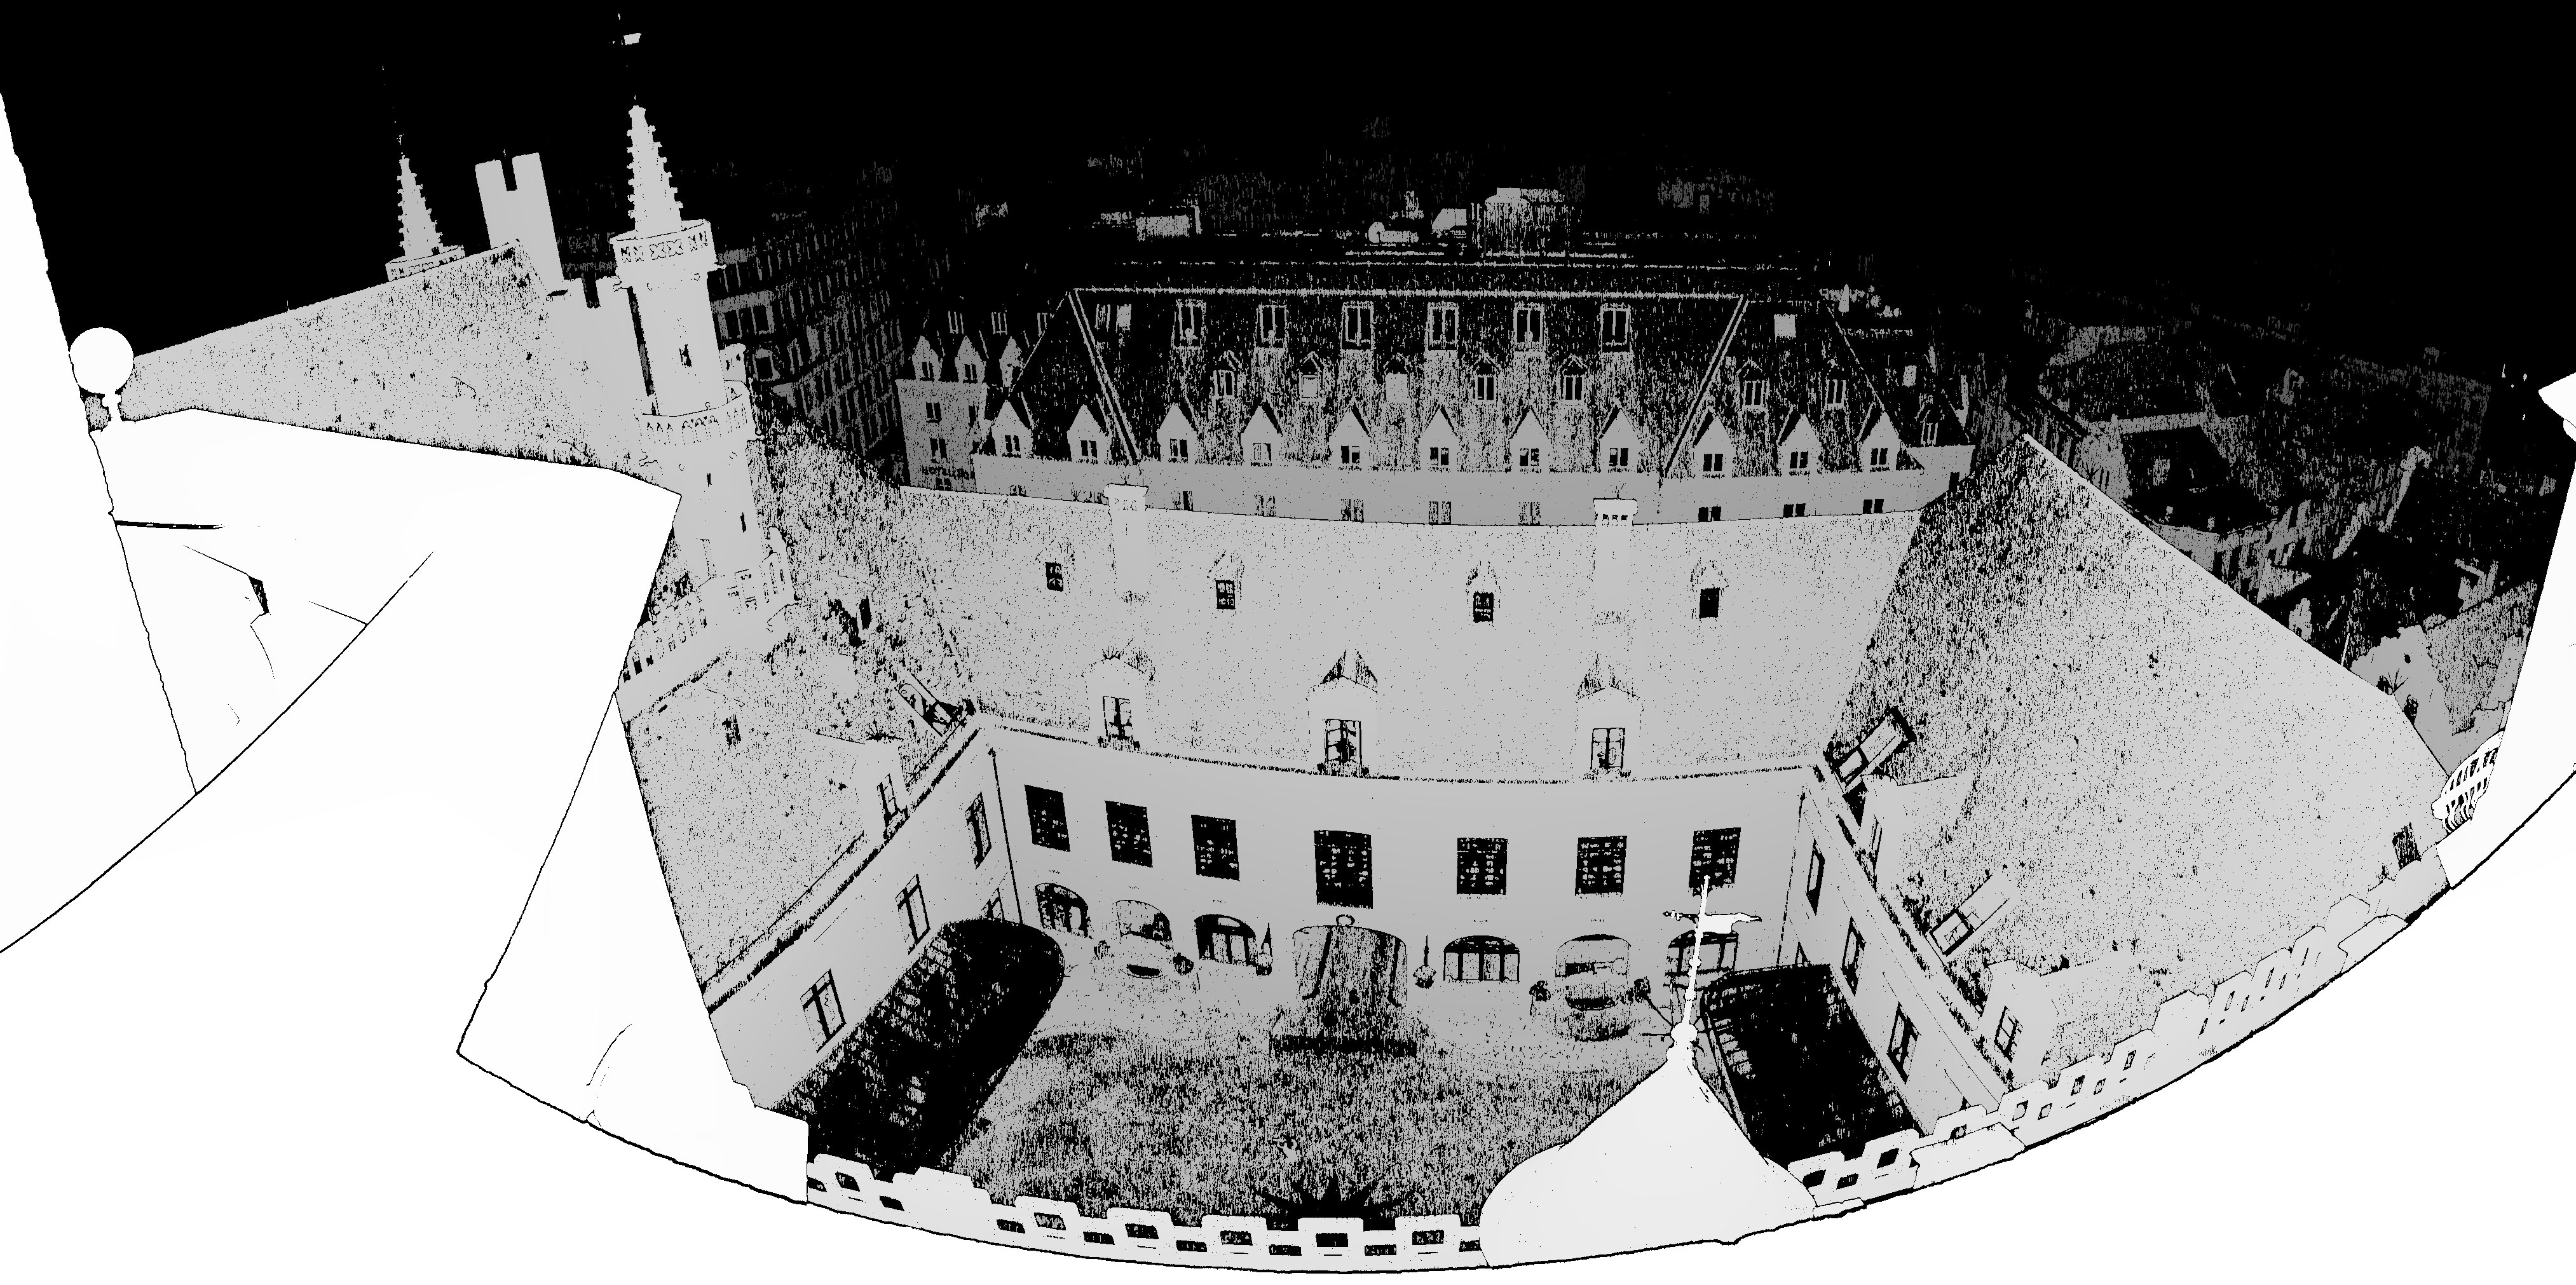
\includegraphics[width=.8\textwidth]{fig/hdv_033_range.jpg}
\label{fig:hdv_033_range}
\caption{Depth view of range image}
\end{figure}

So the range image is a point cloud augmented by two pieces of information: The mapping of pixel coordinates to points $r$ is given for the points in the point cloud. And, the point cloud is set in a coordinate system where the scanner is at origin $(0, 0, 0)$, and it oriented facing the direction $\transpose{(0, 0, -1)}$. This knowledge will allow to make predictions on the dispersion and density of surface points.

\subsubsection{Camera parameters}
As indicated before, when working with point clouds generated from actual 3D scans, the scanner's exact mapping of 3D point coordinates to 2D pixel coordinates is not known. Supposing that the scanner is a laser scanner placed at a fixed position, it corresponds to the mapping of pixel coordinates to azimuth and elevation of the point's spherical coordinates. However when generating artificial point clouds for testing purposes, a model of a scanner (called ``camera'' in the rest of this paper) is made for which those characteristics are well defined.

The following figure shows the 2D equivalents of three possible types of cameras:
\begin{figure}[H]
\begin{subfigure}{.33\textwidth}
	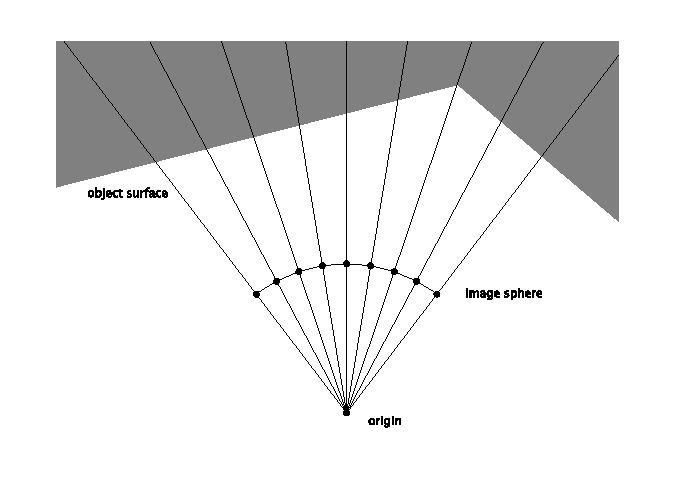
\includegraphics[trim=8mm 1cm 8mm 1cm, crop, width=\linewidth]{fig/cam_range.pdf}
	\caption{Range camera}
\end{subfigure}%
\begin{subfigure}{.33\textwidth}
	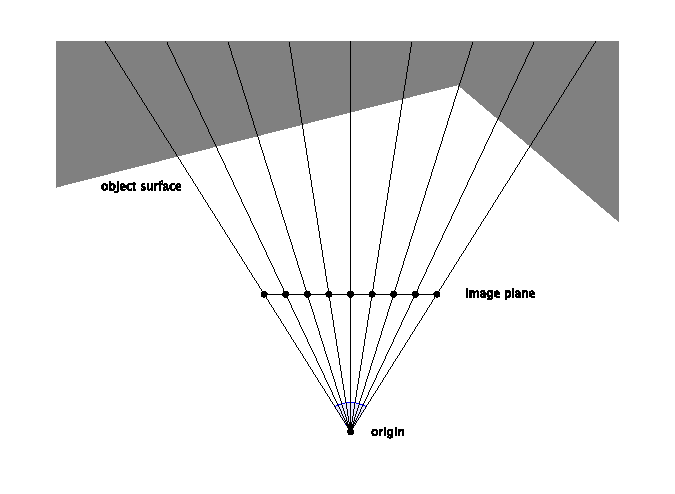
\includegraphics[trim=8mm 1cm 8mm 1cm, crop, width=\linewidth]{fig/cam_perspective.pdf}
	\caption{Perspective camera}
\end{subfigure}%
\begin{subfigure}{.33\textwidth}
	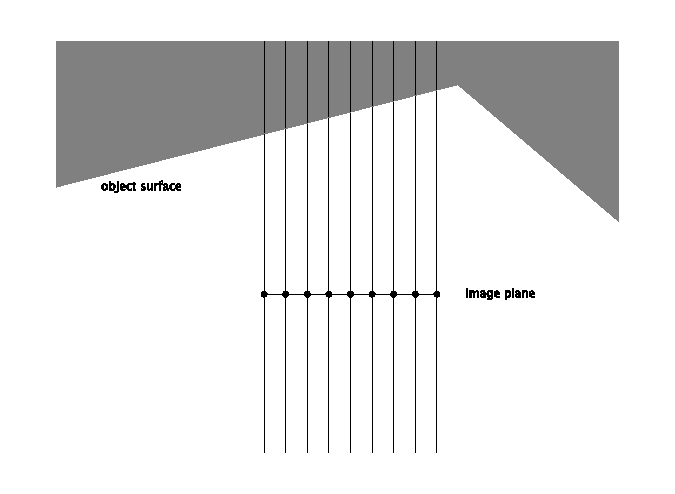
\includegraphics[trim=8mm 1cm 8mm 1cm, crop, width=\linewidth]{fig/cam_parallel.pdf}
	\caption{Parallel camera}
\end{subfigure}
\end{figure}

The \emph{range camera} does a linear mapping from the angle of the ray to the pixel on the image. The image, when put in three-dimensional space such that the rays pass through its pixels, has the shape of a circle arc. For its three-dimensional equivalent, additional complexities occur because of the different possible ways to define spherical coordinates. The field of view can cover the entire range of directions. This model corresponds most closely to a real laser scanner.

For the \emph{perspective camera}, the image is a plane instead of a sphere. This corresponds to the way that photographic cameras take pictures. The resulting image contains some distortion relative to the one from the range camera, as the angles between rays get larger towards the extremities of the field of view. On \emph{parallel camera}, all the rays are parallel. For both the perspective and parallel camera, the mapping from 3D point coordinates to pixel coordinates on the image plane is a linear function and can be described as a multiplication with a $4 \times 4$ matrix in homogeneous coordinates. This is further described in the next chapter. For the range camera, trigonometric functions are necessary to describe the mapping.

For the parallel camera, all rays have the direction of the normal vector $\vec{n}$ of the image plane. When considering only a small subregion of the field of view, the rays can also be considered to be parallel by approximation for the range and perspective cameras, as well as for real 3D scanners. Thus for any small part cropped out of a range image point cloud, the camera can be modeled as a parallel camera. These rays will also by approximation be equidistant from each other, and arranged on a square of rectangular grid on an image plane.

This way the point dispersion on small, locally planar surfaces can be modeled by constructing a parallel camera.


\subsection{3D scanner technology}
In general 3D scanners are devices which probe their physical environment in order to collect information about the shape and possibly appearance of objects.

\subsubsection{Laser rangefinder}
A laser rangefinder is a device which uses a laser beam to find the distance of a physical object. It consists of a laser and an optical sensor pointing in the same direction. A laser beam is sent out to the object, and the \emph{time-of-flight} is measured until the reflected beam is received by the optical sensor. The distance of the object can then be deduced by measuring either \emph{time of flight} or the \emph{phase shift}.

For the former case, a short laser pulse is send out, and the time $\Delta t$ until the reflected light hits the sensor is measured. The distance of the object can then be calculated as $d = \frac{c \, \Delta t}{2}$, where $c$ is the speed of light. Using this procedure long distance measurements of up to 10 kilometers can be taken, at a very high rate. However due to the high speed of light, the precision is limited. Obtaining measurements accurate within more than a few centimeters requires creating very short laser pulses and precise time measurement.

An alternate method is to use a continuous light beam instead of a short pulse, and measure the phase shift between the emitted and the received signal. This allows for measuring the distance in a range within the wavelength of the emitted light. By sampling the cross-correlation of both signals at different time offsets, a value for the phase shift can be obtained.

\subsubsection{Time-of-flight scanner}
Time-of-flight scanners are based on a laser range finder. A 3D scan is performed sequentially measuring the distances in different directions in the field of view. The beam is oriented by rotating the rangefinder or using a mirror system. A \emph{range image} is thus obtained. In spherical coordinates, the radius of each point corresponds to the distance measured by the rangefinder, whereas the azimuth and elevation depends on the direction of the beam. 

These devices are also called \emph{Lidar} scanners, especially in applications other than the scanning of solid object surfaces, as mentioned before. This is by analogy to \emph{Radar} and \emph{Sonar} which operate in a similar way using radio waves and sound waves to detect objects, respectively.

Time-of-flight scanners are \emph{long-range scanners}. They may operate over distances of several kilometers. However due to the high speed of light, they have a relatively low accuracy on the order of millimeters.

\subsubsection{Triangulation scanner}
Another laser-based technique for recording 3D data is to find the spatial location of the laser dot by triangulation. As with the time-of-flight scanner, a laser beam is sequentially projected in different directions onto the object. But instead of measuring the return time of the beam, a it used to track the location of the laser dot on the object surface. The projected two-dimensional position of the laser dot is thus known from both the view point of the laser and the view point of the camera, and the pose of the camera relative to the laser is fixed. These three pieces of information fully determine the three-dimensional location of the laser dot on the object surface.





\section{Operations on point clouds}
This section describes some of the operations that are applied to point cloud data during the post-processing of 3D scans. The point cloud is regarded as an unordered set $P = \{ (x_i, y_i, z_i) \}$. In the next section data structures used to lay the point set out in memory are considered.


\subsection{Basic operations}

\subsubsection{Cropping}
Cropping means to simply remove the points from $P$ that lie outside some geometric region. This region may be a bounding box, a view frustum of a camera or other. It is typically performed manually using point cloud software as a first step in post-processing the 3D scans.

When done on a range image, the coordinate system must be maintained since the camera will still be at the origin, which can be far off the cropped area.

\subsubsection{Fusion}
Since point clouds are unordered point sets, fusing two point clouds corresponds to taking the union of the two sets.

When two point clouds represent different views of the same object and the goal is to get a point cloud the covers a greater part of the object, they must first be \emph{registered} and put into the same coordinate system.

Fusing creates some redundancy in the overlapping parts of the point clouds. Techniques exist to refine the resulting distribution and density of points, as described for example in \cite{Kyos2013}.


\subsubsection{Transformation}
To apply an affine transformation to the object represented by the point cloud, the same transformation matrix is simply applied to each point. The transformation will be relative to the origin point of the point cloud.

When the points are attributed with normal vectors, the linear part of the transformation (i.e. not the translation) also needs to be applied to them.

For point cloud registration, a rigid transformation will be applied to one \emph{loose} point cloud to put it into the coordinate system of the \emph{fixed} point cloud.


\subsubsection{Closest point finding}
Finding for any \emph{position} $(x, y, z)$, the point $p \in P$ closest to it. This can implemented efficiently by using a tree structure representation of the point cloud, as will be described in the next section.

Usually the Euclidian distance between points is used, though for some applications other distance metrics are useful.

\subsubsection{Nearest neighbor finding}
Finding for any \emph{point} $q \in P$ in the point cloud, the point $p \in P$ other than itself that is closest. For many applications it is useful to find the $k$ nearest neighbors, either for one point, or for a whole set of points.

Also here, different data structures allow for implementing this in an efficient manner. Different optimizations are possible here than for the closest point problem, because $q$ must be a point of the point cloud, and not just any position in space.


\subsection{Projection}
Generating a virtual \emph{range image} from the point cloud. As described above, a range image contains only the part of the object that is visible from a given viewpoint. Each point in the range image corresponds to a two-dimensional coordinate on a pixel grid. In range images produced by real 3D scanners, the precise mapping from pixel coordinates to the azimuth and elevation components of the point's spherical coordinates may be unknown.

Here, projection essentially means to simulate the operation on a 3D scanner, with the point cloud replacing the real object. The range image obtained from projecting a point cloud using should ideally be the same as the one obtained from scanning the real object with a scanner that has the same pose and coordinate mapping parameters. However the point cloud contains only a sparse set of point representing the surfaces, and holds no direct connectivity information.

Let $w, h \in \mathbb{N}$ be the width and height of the image. The aim of a projection algorithm is to implement a function $r : [0, w[_{\mathbb{N}} \times [0, h[_{\mathbb{N}} \rightarrow P \cup \{ \epsilon \}$, which associates to each image pixel a point from the point cloud $P$, or the invalid point $\epsilon$. 

Let $\mathbf{proj}_{C} : \mathbb{R}^3 \rightarrow \mathbb{N}^2 \cup \{ \epsilon \}$ be the function used to map 3D coordinates to pixel coordinates. $C$ represents the pose and parameters of the virtual camera. So $(0, 0) \leq \mathbf{proj}(\cdot) < (w, h)$. For each image coordinate $(x_i, y_i)$, the region of space where points would map onto that pixel is given by $\{ p \in \mathbb{R}^3 : \mathbf{proj}_{C}(p) = (x_i, y_i) \}$. In the case of perspective projection, it will have the shape of a thin square-base frustum extending from the camera point to infinity. In orthogonal projection, is instead corresponds to a thin cuboid. The discrete subset of points from the point cloud $P$ which lie in that region is given by $P_{(x_i,y_i)} = \{ p \in P : \mathbf{proj}_{C}(p) = (x_i, y_i) \}$.

Figure \ref{fig:pp_projection} shows the situation in 2D for a perspective position. Two surface parts of the object lie inside the frustum. The further one is called $A$ and the closer one $B$.

\begin{figure}[h]
\center
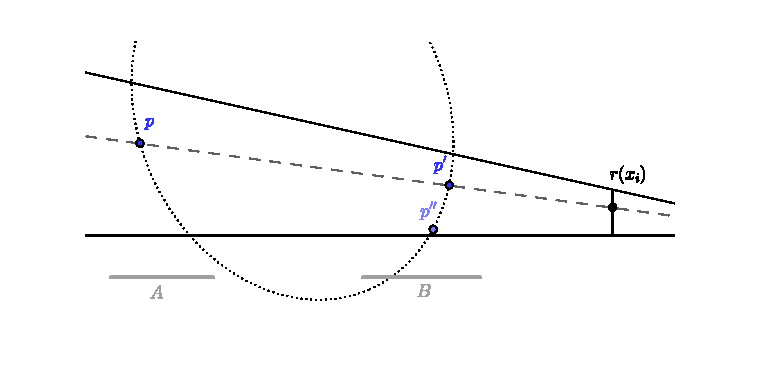
\includegraphics[width=.8\textwidth]{fig/pp_projection.pdf}
\label{fig:pp_projection}
\caption{Illustration of point cloud to range image projection in 2D}
\end{figure}

A simple approach to define the function $r$ is to let $r(x_i, y_i)$ be the point in $P_{(x_i,y_i)}$ that is closest to the camera, or $\epsilon$ when $P_{(x_i,y_i)}$ is empty. If $P_{(x_i,y_i)}$ was not a discrete set, but instead an uncountable set of surface points, it would be guaranteed that the chosen point $p$ if not occluded by another point $p'$ lying in front of it, because $p'$ would necessarily also be in $P_{(x_i,y_i)}$.

Choosing the closest point is not necessarily the best approach. Another point $p''$ might be a better candidate, when evaluating additional attributes of the points. Also the closest point may be an outlier located in front of $B$. Another approach can be to group several points and generate a new one. The important thing is that the point lies on surface $B$.

But because $P_{(x_i,y_i)}$ are discrete sets, if the point density is not high enough, it can occur that no point in it lies on surface $B$, and so instead one in $A$ would be chosen.



\subsection{Registration} \label{sec:pc_registration}
Given two point clouds $P$ and $Q$ that represent the same object, find a translation and rotation that will put both point clouds into the same coordinate system, and thus align the corresponding parts. $P$ and $Q$ are be taken from different poses, so different parts of the object are occluded in the two point clouds.

For example to obtain a full point cloud of a solid object, it needs to be scanned from different sides. Before it can be merged into a full point cloud, the precise relative poses of the scans need to be known. The aim of a registration algorithm is to compute an estimation of those poses.

Many different methods exist. A large survey of registration methods is given in chapter \ref{ch:pcreg}.



\subsection{Other operations}

\subsubsection{Computation of normal vector}
Computing the normal vector of the surface at a given point $p \in P$. Different approaches exist, and because the surface is unknown there is not necessarily a best method or a clear way to evaluate its accuracy.

One basic way is to compute the $k$ nearest neighbors for some value $k$, and then take the normal vector of a plane fitted to those $k + 1$ points. 

Other per-point values such as a local density or curvature measure can be useful, and a version for those two will be defined chapter \ref{ch:large_model}.


\subsubsection{Image-to-cloud registration}
Wrapping a photographic image on a point cloud, for example with the goal of attributing colors to points from a raw scan. This involves photogrammetric and image analysis techniques for finding correspondences between the point cloud and the image.


\subsubsection{Meshing}
Adding connectivity to the points, by constructing a triangular mesh that joins together neighboring points on the same surfaces. 




\section{Data structures for point clouds}
Even though a point cloud is defined as an unordered set of points, for it to be processed algorithmically the data needs to be laid out in a certain way in computer memory. The lack of an order relation between the points provides for great flexibility. At the same time, the structure of a point cloud is that of a sparse discrete set of points embedded in three-dimensional continuous space, whereas computer memory is a dense, discrete array of bits.

Compromises need to be made in laying out the data in a way such that the required operations can be performed efficiently. 

...........................


\section{Preliminary mathematics}
This section presents some mathematical results and methods that are used in the text to follow.

\subsection{Transformation matrices and homogeneous coordinates}
Positions in three-dimensional space can be represented using cartesian coordinates. Let $O$ be an origin point in space, and let $\vec{i}, \vec{j}, \vec{k}$ be three orthogonal vectors of norm $1$. Then $\vec{p} = (x, y, z)$ represents the position $O + x \, \vec{i} + y \, \vec{j} + z \, \vec{k}$. The vectors $\vec{o}, \vec{i}, \vec{j}, \vec{k}$ define the coordinate system.

A point cloud as defined as a set of points, where each one has a position and possible additional attributes. The positions in one point cloud are all set in the same coordinate system. When the points are attributes with normal vectors, or other vector-type attributes, this is also true for them. Applying a transformation $\matr{T}$ to a point cloud means applying that transformation to the position, and if applicable to any vector-type attributes of it.

\subsubsection{Classification}
The transformations used here are classified as follows:

\begin{figure}[h]
\center
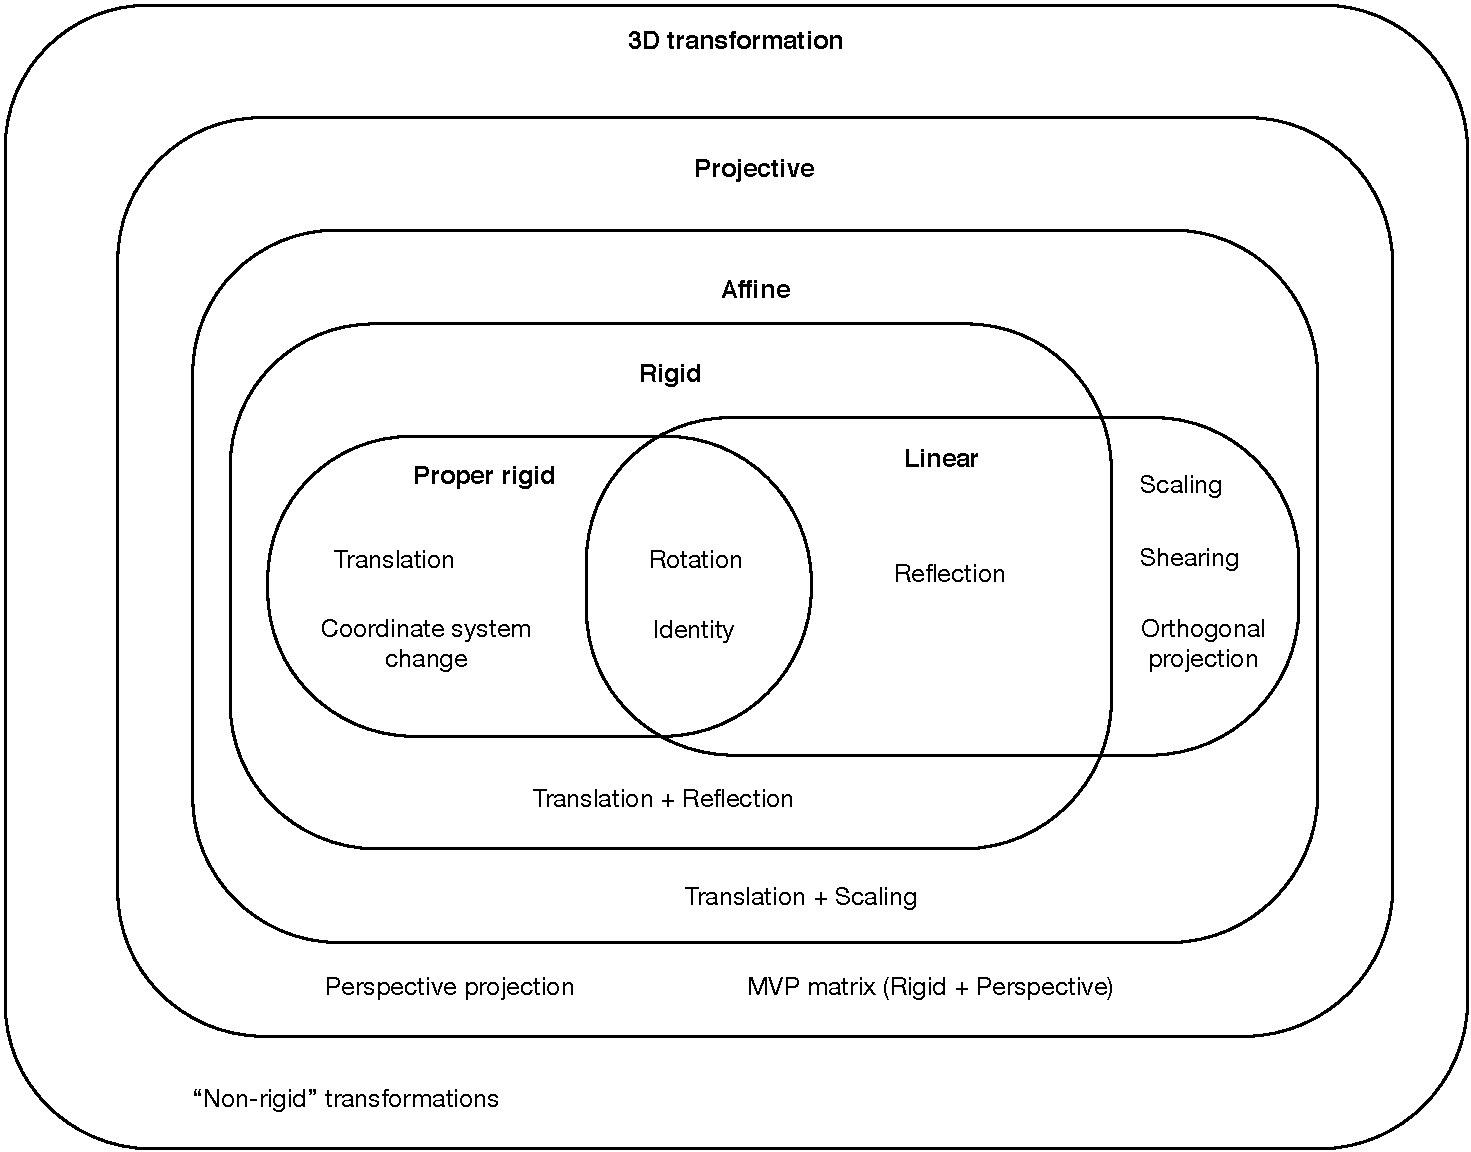
\includegraphics[width=.8\textwidth]{fig/transformations_venn.pdf}
\caption{Venn diagram of three-dimensional transformations}
\end{figure}

\emph{Linear} transformations correspond to a linear recombination of the three coordinates, and can be expressed using a $3 \times 3$ transformation matrix. \emph{Affine} transformations are linear transformation with an additional translation. A \emph{rigid} transformation is an affine transformation where the linear part corresponds to an orthogonal matrix. It preserves the distance between every pair of points. \emph{Proper rigid} transformations exclude shearing, and consist of a rotation and a translation. They correspond to the movement an object can make in three-dimensional space without altering its shape. A \emph{projective} transformation is an affine transformation, followed by a division of the three coordinates by one same linear combination of the coordinates. It can for instance express perspective projections. Additionally, the term \emph{non-rigid} transformation is sometimes used in the context of point cloud registration, to express any transformation (not necessarily affine) that alters the shape of the model.

Transformations can be combined into a conjunction of transformations, which would be classified into the lowest common class of its components. For instance a translation followed by a reflection would be a rigid transformation that is neither linear nor proper rigid. Conjunctions of transformations are in general not commutative, but all possible orders of application belong to the same class.

\subsubsection{Linear transformation}
A linear transformation is one where each coordinate of a point is mapped to a linear combination of the three coordinates. As such it can be expressed using a $3 \times 3$ matrix, and applying the transformation corresponds to multiplying this matrix $\mat{T}$ by column vector formed by the point coordinates.
\begin{equation}
\left[ \begin{matrix}
	t_{1,1} & t_{1,2} & t_{1,3} \\
	t_{2,1} & t_{2,2} & t_{2,3} \\
	t_{3,1} & t_{3,2} & t_{3,3}
\end{matrix} \right] \times
\left[ \begin{matrix} x \\ y \\ z \end{matrix} \right] = 
\left[ \begin{matrix}
	t_{1,1} \, x + t_{1,2} \, y + t_{1,3} \, z \\
	t_{2,1} \, x + t_{2,2} \, y + t_{2,3} \, z \\
	t_{3,1} \, x + t_{3,2} \, y + t_{3,3} \, z
\end{matrix} \right]
\end{equation}
So in a transformation $\vec{p'} = \matr{T} \, \vec{p}$, $t_{i,j}$ indicates the coefficient of the $j$-th coordinate of $\vec{p}$ in the $i$-th coordinate of $\vec{p'}$. As a consequence the origin $(0, 0, 0)$ is a fixed point in linear transformation. Linear transformations can for example express a rotation, a shearing, a reflection, or an orthogonal projection. Because of the associativity of matrix multiplication, the composition of linear transformations can be expressed in one single linear transformation matrix. First applying $\matr{T_1}$ followed by $\matr{T_2}$ is the same as applying $\matr{T_2} \times \matr{T_1}$, because
\begin{equation}
	\vec{p'} = \matr{T_2} \, ( \matr{T_1} \, \vec{p} ) = (\matr{T_2} \, \matr{T_1}) \, \vec{p}
\end{equation}

Also, the inverse transformation is expressed by the inverse of the transformation matrix $\matr{T^{-1}}$. As mentioned, the conjunction of two linear transformations is non-commutative, just like the underlying matrix multiplication.

\subsubsection{Rotation}
In two dimensional euclidian geometry, a rotation around the origin point $(0, 0)$ with angle $\theta$ is expressed by the linear transformation matrix
\begin{equation}
\matr{R}_{\theta} = \left[ \begin{matrix}
	\cos \theta & - \sin \theta \\
	\sin \theta & \cos \theta
\end{matrix} \right]
\label{eq:rotation-matrix-2d}
\end{equation}
This can be derived using the geometric definition of the trigonometric functions. In three-dimensional additionally a plane of rotation, of equivalently an axis of rotation needs to be specified. The linear transformation matrices for the \emph{elemental rotations} around the \emph{x}, \emph{y} or \emph{z} axis can be deduced from \ref{eq:rotation-matrix-2d} by keeping one coordinate unchanged and applying the 2D rotation on the plane formed by the other two:
\begin{equation}
\matr{R}_{\theta}^x = \left[ \begin{matrix}
	1 & 0 & 0 \\
	0 & \cos \theta & - \sin \theta \\
	0 & \sin \theta & \cos \theta
\end{matrix} \right]
\hspace{1cm}
\matr{R}_{\theta}^y = \left[ \begin{matrix}
	\cos \theta & 0 & \sin \theta \\
	0 & 1 & 0 \\
	- \sin \theta & 0 & \cos \theta
\end{matrix} \right]
\hspace{1cm}
\matr{R}_{\theta}^z = \left[ \begin{matrix}
	\cos \theta & - \sin \theta & 0 \\
	\sin \theta & \cos \theta & 0 \\
	0 & 0 & 1
\end{matrix} \right]
\end{equation}

\subsubsection{Euler angles}
One common way to express a three-dimensional rotation is using \emph{Euler angles}, that is, the angles by which to rotate around those three axis. For example, $(\phi, \theta, \psi)$ may express the rotation $\matr{R}_{\phi}^x \, \matr{R}_{\theta}^y \, \matr{R}_{\psi}^z$. Because of the non-commutativity, many different conventions are possible: The three elementary rotations can be applied in different orders, such as \emph{x-y-z}, \emph{z-y-x} or \emph{x-y-z}. Also combinations of only two elementary rotations like \emph{x-y-x} or \emph{z-x-z} are possible, where the same axis used for the first and third rotation. In expression like $\matr{R}_{\phi}^x \, \matr{R}_{\theta}^y \, \matr{R}_{\psi}^z$, the three elementary rotations are \emph{intrinsic}: The second rotation rotates around the new \emph{y} axis, which has already been displaced from the first rotation. In an \emph{explicit} conventions, all three rotations instead take place in a fixed coordinate system.

The terms \emph{yaw}, \emph{pitch} and \emph{roll} are commonly used to name the three rotation angles. Given an object pointing into a certain direction in space, such as a camera or a moving vehicle, \emph{roll} refers to a rotation around the axis in which it is pointing. \emph{Pitch} is a rotation around its relative horizontal axis, and \emph{yaw} around its relative vertice axis. For example, a \emph{pitch} rotation of an aircraft would make it fly upwards or downwards.

Besides the many possible conventions, another problem with Euler angles is the \emph{gimbal lock} phenomenon, where two components can end up representing a rotation around the same axis.

Because of gimbal lock, and because the angles are taken modulo $2\pi$, small changes in a rotation do not always correspond to small changes in the Euler angles. This makes them unsuited for processing rotations algorithmically and for solving optimisation problems. Instead, a good alternative to directly working with rotation matrices is to use quaternions, which express the rotation using $4$ real values.

\subsubsection{Quaternions}
...

\subsubsection{Rotation around an axis}

\subsubsection{Rotation between two vectors}

\subsubsection{Affine transformation}
Translations are not linear transformations, because they add a constant term to each coordinate of $\vec{p'}$. An \emph{affine} transformation corresponds to a linear transformation followed by a translation: $\vec{p'} = \matr{T} \, \vec{p} + \vec{t}$. Let $\vec{p'} = \matr{T_1} \, \vec{p} + \vec{t_1}$ and $\vec{p''} = \matr{T_2} \, \vec{p'} + \vec{t_2}$ be the expressions of two subsequent affine transformation to apply to $\vec{p}$.
\begin{equation}
	\vec{p''} = \matr{T_2} \, (\matr{T_1} \, \vec{p} + \vec{t_1}) + \vec{t_2} = (\matr{T_2} \, \matr{T_1}) \, \vec{p} + (\matr{T_1} \vec{t_1} + \vec{t_2})
\end{equation}
So a composition of multiple affine transformations is still an affine transformation, but the translation vectors cannot be simply added up. It can be seen that the composition is again non-commutative, except for the case when $\matr{T_2} = \matr{T_1} = \matr{I}$, that is, when both transformations are translations only.

Also if the translation component is applied \emph{before} the linear component (instead of \emph{after} it), it represents a different affine transformation:
\begin{equation}
	\matr{T} \, (\vec{p} + \vec{t}) = \matr{T} \, \vec{p} + \matr{T} \, \vec{t} \neq \matr{T} \, \vec{p} + \vec{t}
\end{equation}

\subsubsection{Rigid transformation}
The subclass of affine transformation where $\matr{T}$ is an orthogonal matrix are the rigid transformations. By definition, its row vectors, and its column vectors are orthogonal unit vectors. Orthogonal matrices preserve the dot product of vectors, and as a consequence distances and angles between any two pairs of points are preserved. Orthogonal matrices represent either a rotation or a reflection, and its determinant $\det(\matr{T})$ is always either $+1$ for a rotation or $-1$ for a reflection. This is a necessary but not sufficient condition, as there are also non-orthogonal matrices with determinant $+1$ or $-1$. So a rigid transformation can be a translation, rotation, reflection, or any composition thereof.

A proper rigid transformation is defined as a rigid transformation for which $\matr{T}$ is a rotation matrix. It always consists of a rotation and a translation, and any composition of proper rigid matrices can be reformulated as a single rotation and translation:
\begin{equation}
	\matr{R_2} \, (\matr{R_1} \, \vec{p} + \vec{t_1}) + \vec{t_2} = (\matr{R_2} \, \matr{R_1}) \, \vec{p} + (\matr{R_2} \, \vec{t_1} + \vec{t_2})
\end{equation}
Where $\matr{R_2} \, \matr{R_1}$ is also an orthogonal matrix, it being the composition of two rotations.

Proper rigid transformations correspond to the ways a real object can be moved in three-dimensional space without altering its shape. As such, they can be used to represent the position and orientation of an object.

In the following text, the term ``rigid transformation'' will always refer to a proper rigid transformation.

In most use cases involving three-dimensional geometry, non-proper rigid transformations are rarely used since they change the handedness of an object, which is in reality not possible in three-dimensional space. In fact, with a fourth spatial dimension it would be possible with a 4D rotation that temporarily pulls the object out of the three-dimensional subspace. This process would not alter the object's internal structure. But while both the start and end state would be possible in 3D space, the intermediary steps are not, and movements in reality are always continuous.

\subsubsection{Homogeneous coordinates}
In order to simplify calculations and notation, it is natural to use \emph{homogeneous coordinates}. They allow for affine and projective transformations to be written using a single $4 \times 4$ matrix.

Formally, a vector $\homvec{v}$ in homogeneous coordinates corresponds to a vector $\vec{v}$ in cartesian coordinates iff
\begin{equation}
	\homvec{v} = \colvecT{x, y, z, w}
	\hspace{1cm}\mathrm{and}\hspace{1cm}
	\vec{c} = \colvecT{\frac{x}{w}, \frac{y}{w}, \frac{z}{w}}
\end{equation}

The conversion from homogeneous to cartesian coordinates consists of an element-wise division by the fourth component $w$ of the vector itself. This non-linear operation cannot be represented by cartesian matrix multiplications alone. The equivalent in homogeneous coordinates of an affine transformation given by the linear transformation $\matr{L}$\footnote{Using $\matr{L}$ here instead of $\matr{T}$ to have different lowercase letters.}, and the translation vector $\vec{t}$, where the linear transformation is applied before the translation, is the $4 \times 4$ matrix
\begin{equation}
	\hommatr{T} = \left[ \begin{matrix}
		l_{1,1} & l_{1,2} & l_{1,3} & t_1 \\
		l_{2,1} & l_{2,2} & l_{2,3} & t_2 \\
		l_{3,1} & l_{3,2} & l_{3,3} & t_3 \\
		0 & 0 & 0 & 1
	\end{matrix} \right]
\end{equation}
A distinction is made between positions and vectors: When transforming a position, with the linear transformation is applied, followed by the translation. For vectors on the other hand, only the linear transformation is applied. A vector does not have a position in space, but only a direction and norm. Its coordinates represent the position of its end point, assuming that its start point is at $\colvecT{0, 0, 0}$. For example when applying a rigid transformation to a point cloud where points are attributed with surface normal vectors, the point positions should get rotated and then translated. The normal vectors should be rotated the same way, but no translation vector should be added to them.

Positions are converted into homogeneous coordinates by adding an extra component $w = 1$, whereas for vectors an extra component $w = 0$ is added. The three first components $x, y, z$ remain the same. It can be seen that
\begin{equation}
\left[ \begin{matrix}
	x \\ y \\ z \\ 1
\end{matrix} \right] \times  \left[ \begin{matrix}
	l_{1,1} & l_{1,2} & l_{1,3} & t_1 \\
	l_{2,1} & l_{2,2} & l_{2,3} & t_2 \\
	l_{3,1} & l_{3,2} & l_{3,3} & t_3 \\
	0 & 0 & 0 & 1
\end{matrix} \right] = \left[ \begin{matrix}
	l_{1,1} \, x + l_{1,2} \, y + l_{1,3} \, z + t_1 \\
	l_{2,1} \, x + l_{2,2} \, y + l_{2,3} \, z + t_2 \\
	l_{3,1} \, x + l_{3,2} \, y + l_{3,3} \, z + t_3 \\
	1
\end{matrix} \right] \coreq \left[ \begin{matrix}
	l_{1,1} \, x + l_{1,2} \, y + l_{1,3} \, z + t_1 \\
	l_{2,1} \, x + l_{2,2} \, y + l_{2,3} \, z + t_2 \\
	l_{3,1} \, x + l_{3,2} \, y + l_{3,3} \, z + t_3 \\
\end{matrix} \right]
\end{equation}
In the case where $w = 0$, the components of $\vec{t}$ get removed. In the case of affine transformations, the last row of the homogeneous matrix is always $\rowvec{0, 0, 0, 1}$, and no division takes place. For perspective projections, a division by the $z$ component will compute foreshortening.

Because here an affine or projective transformation is applied by single matrix multiplication, is follows that any composition of those matrices can be represented using the matrix product of multiple $4 \times 4$ matrices.

\subsubsection{Pose}
This position and orientation of an object in space is called its \emph{pose}. A pose is also a cartesian coordinate system. Coordinates as well as other poses are always defined relative to such a coordinate system.

In any sufficiently complex three-dimensional environment, it becomes natural to define the positions and orientations of object relative to each other, and not in a single global coordinate system. 3D modelling software such as \emph{Blender} typically implement a tree-structure of objects, in which the pose of each object is defined relative to its parent. A similar software system was written for this project.

The problem of 3D scan registration treated in this paper is precisely to find the pose from which a scan was taken, relative to another scan, and the output of any point cloud registration algorithm is a rigid transformation matrix.

A pose corresponds to an orthonormal coordinate system which is defined by tuple $S = \langle O, \vec{i}, \vec{j}, \vec{k} \rangle$ where $O$ is the origin point, and $\vec{i}, \vec{j}, \vec{k}$ three orthogonal vectors with $\|\vec{i}\| = \|\vec{j}\| = \|\vec{k}\| = 1$. The origin point and the vectors of a coordinate system are defined within its \emph{parent} coordinate system. The root coordinate system in that tree is called \emph{world space}. For an \emph{identity} coordinate system, $O = (0, 0, 0)$, $\vec{i} = \colvecT{1, 0, 0}$, $\vec{j} = \colvecT{0, 1, 0}$ and $\vec{k} = \colvecT{0, 0, 1}$.

A pose can also be expressed using the \emph{transform-to-parent} rigid transformation $\matr{M}$, which transforms the coordinates of points or vectors expressed in its coordinate system $S_i$, into the coordinates of the same point of vector in its parent coordinate system $S_{i-1}$. Equivalently, the \emph{transform-from-parent} rigid transformation is its inverse $\matr{M^{-1}}$. Then
\begin{equation}
	O_{i} = \matr{M^{-1}} \, O_{i-1}
	\hspace{1cm}
	\vec{i_{i}} = \matr{M^{-1}} \, \vec{i_{i-1}}
	\hspace{1cm}
	\vec{j_{i}} = \matr{M^{-1}} \, \vec{j_{i-1}}
	\hspace{1cm}
	\vec{k_{i}} = \matr{M^{-1}} \, \vec{k_{i-1}}
\end{equation}
where the distinction between positions and vectors using homogeneous coordinates is made.



...

\subsection{Least squares method}
The least squares method is a way to calculate an approximate solution to an overdetermined system. For example the equation $y = ax + b$ of a line that crosses two points $(x_1, y_1)$ and $(x_2, y_2)$ can easily be calculated by solving a linear system with 2 equations and 2 unknowns. But if there are 3 or more points, there is no solution unless the points are perfectly aligned. Here a least squares solution would be the line which minimizes the sum of the squares of the distances of the points to itself.

Formally, let $\{ (x_i, y_i) \}$ be a set of $n$ data points. $x_i$ are independent variables and $y_i$ dependent variables found by observation. Both $x_i$ and $y_i$ can be vectors. For example the problem of fitting a plane to a set of 3D points may be modelled with $x_i$ being a data point's X coordinate, and $\vec{y_i}$ that data point's Y and Z coordinates.

The goal is to find a vector of parameters $\beta$ that define a model $\hat{y}_i = f_{\beta}(x_i)$. Because in general there is no $f_{\beta}$ for which $\forall i, \hat{y}_i = y_i$, one searches a solution that minimizes the sum of the squared residuals:
\begin{equation}
\hat{\beta} = \argmin_{\beta} S \hspace{7mm} \text{where} \hspace{7mm} S = \sum_{i=1}^{n} (y_i - \hat{y}_i)^2
\end{equation}
For the example where the model is a line, one can define $\beta = (a, b)$ and $f_{\beta}(x) = ax + b$. Then the residual would be the vertical distance of a point to a line. It is also possible to define a linear expression of $f_{\beta}$ by which the orthogonal distances of the points to the lines is minimised. Many similar geometrical fitting problems can be solved in this manner, such as fitting a plane, circle, sphere, or other object to a set of points. \cite{Eber1999}

\subsubsection{Linear least-squares}
In general, a solution for least square problems can be computed by setting the gradient $\nambla S$ to zero. Since the terms $y_i$ are constant, this becomes for each component $\beta_j$:
\begin{equation} \label{eq:lsq_sol}
\frac{\partial S }{\partial \beta_j} = -2 \sum_{i=1}^{n} \frac{\partial f_{\beta}(x)}{\partial \beta_j} = 0
\end{equation}

If $f_{\vec{\beta}}$ is a linear combination of the parameters $\vec{\beta}$, then a closed form expression for the solution exists. Let there be $n$ data points $(x, y)$, where $x$ are vectors of $m$ components, and $y$ real numbers. (Here the subscript refers to the component of the vector $x$, not the index of the data point). $\beta$ will also have $m$ components. The function $f_{\beta}$ is of the form
\begin{equation} \label{eq:lsq_linf}
f_{\beta}(x) = \beta_1 \, x_1 + \beta_2 \, x_2 + \dots + \beta_m \, x_m
\end{equation}
For the example of fitting a line to a set of 2D points, one would add a second component to the dependent variables which is always set to $1$, so as to get back to $f_{\beta}(x) = ax + b$.

The overdetermined system to solve can be written in matrix form
\begin{equation}
\matr{X} \, \hat{\beta} = \vec{y}
\end{equation}
where $\matr{X}$ is a $n \cross m$ matrix. Each row corresponds to a data point, and each component per row corresponds to the $j$-th component $x_j$ of the dependent variable of that data point. The sum of squares $S$ to minimize becomes
\begin{equation}
S = \sum_{i=1}^{n} \| y_i - \sum_{j=1}^{m} X_{i,j} \beta_{j} \|^2 = \| y - \matr{X} \, \vec{\beta} \|^2
\end{equation}
From \ref{eq:lsq_linf}, the partial derivative of a residual becomes
\begin{equation} \label{eq:lsq_linr}
\frac{\partial (y_i - f_{\beta}(x))}{\partial \beta_j} = - X_{i,j}
\end{equation}
Putting \ref{eq:lsq_linr} into \ref{eq:lsq_sol} and rearranging the expression, one obtains the \emph{normal equations}:
\begin{equation}
\sum_{i=1}^{n} \sum_{k=1}^{m} X_{ij} \, X_{ik} \, \hat{\beta}_k = \sum_{i=1}^{n} X_{ij} \, y_{i}
\hspace{7mm} \text{for} \hspace{7mm}
j = 1, 2, \dots, m
\end{equation}
Written in matrix form:
\begin{equation}
(\transpose{\matr{X}} \, \matr{X}) \, \hat{\beta} = \transpose{\matr{X}} \, \vec{y}
\end{equation}
And so the parameters $\hat{\beta}$ for which $f_{\hat{\beta}}(x)$ is a least squares solution to a linear system can be computed using the closed form expression
\begin{equation}
\hat{\beta} = (\transpose{\matr{X}} \, \matr{X})^{-1} \, \transpose{\matr{X}} \, \vec{y}
\end{equation}

\subsubsection{Non-linear least squares}
When $f_{\beta}$ is not a linear combination of $x_1, x_2, \dots, x_m$ a closed form solution is generally not possible. Instead it can be computed using the \emph{Gauss-Newton algorithm}, by iterative numerical approximation.

\subsubsection{Weights}
The least squares methods finds a solution for which the squared residual $(y_i - \hat{y}_i)^2$ is minimized and evenly distributed among all data points. Weights can be added to introduce bias towards higher weight data points, letting their residual become smaller and the others' larger.

For each data point a \emph{weight} $w_i \in \mathds{R}$ is defined. When $w_i = k \times w_j$ for $k \in \mathds{N}$, the effect is the same as adding $k$ times the data point $(x_i, y_i)$. With weights, the sum to minimize is
\begin{equation}
S = \sum_{i=1}^{n} w_i \, (y_i - \hat{y}_i)^2
\end{equation}
By distributivity, when all $w_i$ become $\lambda w_i$, $S$ becomes $\lambda S$, which doesn't change the minimization problem. Supposing that $w_i$ are rational numbers (which can approximate real numbers to an arbitrary precision), then there exists $\lambda$ such that $\lambda w_i \in \mathds{N}$. This justifies the previous statement about data points duplication. 

\subsubsection{}

\subsection{Point set alignment using singular value decomposition} \label{sec:lsq_align}
For point cloud registration, corresponding points $(\vec{p_i}, \vec{q_i})$ of two point clouds are used to find a rigid transformation $\matr{M}$ that aligns the two point clouds. When there are exactly three pairs of points, an exact solution can be found using vector algebra. \cite{Horn1986} For more than three points, a least squares solution can be found.

Here $f_{\beta}(\vec{q}) = \matr{M} \, \vec{q} = \matr{R} \, \vec{q} + \vec{t}$ is the function that applies the sought after rigid transformation. The parameter vector $\beta$ has 6 components, three for the translation and three for the rotation. $\matr{R}$ is the rotation matrix and $\vec{t}$ the translation vector. The independent variable is $\vec{q_i}$, a 3-vector with the coordinates of a point. The dependent variable is $\vec{p_i}$, also a 3-vector with the coordinates of the corresponding point from the other point cloud.

Because the independent variables are vectors, the residuals to minimize are the squares of the norms of the vector differences. The sum $S$ to minimize becomes
\begin{equation}
S = \sum_{i=1}^{n} w_i \, \| \vec{p_i} - (\matr{R} \, \vec{q_i} + \vec{t}) \|^2
\end{equation}

The assumption is that both point sets $\{ p_i \}$ and $\{ q_i \}$ have approximately the same constellation but are in a different pose. For registration, first they need to be translated so as to make one common point coincide, and then they can be aligned by rotating one point set around that point. As a common point, the centroids of both point clouds are chosen:
\begin{equation}
\vec{c_p} = \frac{1}{N} \, \sum_{i=1}^{n} \vec{p_i}
\hspace{7mm} \text{and} \hspace{7mm}
\vec{c_q} = \frac{1}{N} \, \sum_{i=1}^{n} \vec{q_i}
\end{equation}
Because the constellations are not exactly equal, this choice evenly distributes the error. Also, when the shape that the points form around the centroid point is roughly that of a sphere (their distances from the centroid do not vary too much), the rotating around the centroid will move each point by about the same amount, again evening out the error. 

A rotation matrix $\matr{R}$ expressed a rotation around the origin. In order to simplify the problem, both point clouds are first translated to put the centroid at origin. So $\forall i$ one defines
\begin{equation}
\vec{p'_i} = \vec{p_i} - \vec{c_p}
\hspace{7mm} \text{and} \hspace{7mm}
\vec{q'_i} = \vec{q_i} - \vec{c_q}
\end{equation}
and the minimization problem becomes
\begin{equation} \label{eq:lsq_align_meaneds}
S' = \sum_{i=1}^{n} w_i \, \| \vec{p'_i} - \matr{R} \, \vec{q'_i} \|^2
\end{equation}
Since $\vec{t}$ was applied after $\matr{R}$, this does not change the meaning of $\matr{R}$.

Different approaches exist for computing $\matr{R}$ in constant time, that is without the need for iterative numerical approximation. \cite{Horn1986} describes a solution whereby $\matr{R}$ is represented as a unit quaternion. This was used in the original description of the ICP algorithm (see \label{sec:icp}) in \cite{Besl1992}. \cite{Loru1995} gives a comparison of four methods, also in the context of the ICP algorithm. Probably the most commonly implemented approach is the following, which is based on singular value decomposition.

Using some matrix algebra, \ref{eq:lsq_align_meaneds} becomes
\begin{equation}
S' = \sum_{i=1}^{n} w_i \, \| \vec{p'_i} \|^2 + w_i \, \| \vec{q'_i} \|^2 - 2 \, w_i \, \transpose{\vec{q'_i}} \, \matr{R} \, \vec{p'_i}
\end{equation}
The first and second terms do not depend on $\matr{R}$, hence the problem is reduced to maximizing $\sum_{i} w_i \, \transpose{\vec{q'_i}} \, \matr{R} \, \vec{p'_i}$.

Let $\matr{W} = \text{diag}(w_1, w_2, \dots, w_n)$, and let $\matr{P}$ and $\matr{Q}$ be $3 \times n$ matrices composed of the $n$ column-vectors. One has
\begin{equation}
\matr{W} \, \transpose{\matr{Q}} = \left[ \begin{matrix}
	\-- & w_1 \, \transpose{\vec{q'_1}} & \--\\
	\-- & w_2 \, \transpose{\vec{q'_2}} & \--\\
	& \vdots & \\
	\-- & w_n \, \transpose{\vec{q'_n}} & \--
\end{matrix} \right]
\hspace{7mm} \text{and} \hspace{7mm}
\matr{R} \, \matr{P} = \left[ \begin{matrix}
	| & | & & |\\
	\matr{R} \, \vec{p'_1} & \matr{R} \, \vec{p'_2} & \hdots & \matr{R} \, \vec{p'_n}\\
	| & | & & |
\end{matrix} \right]
\end{equation}
It can be seen that
\begin{equation}
\sum_{i=1}^{n} w_i \, \transpose{\vec{q'_i}} \, \matr{R} \, \vec{p'_i} = \text{tr}(\matr{W} \, \transpose{\matr{Q}} \, \matr{R} \, \matr{P})
\end{equation}
Where the trace $\text{tr}$ is the sum of the diagonal entries of a matrix. Because $\matr{A} \matr{B} = \transpose{(\matr{B} \matr{A})}$ and the trace is invariant under the transpose,
\begin{equation}
\text{tr}((\matr{W} \, \transpose{\matr{Q}}) \, (\matr{R} \, \matr{P})) = \text{tr}((\matr{R} \, \matr{P}) \, (\matr{W} \, \transpose{\matr{Q}})) = \text{tr}(\matr{K} \, \matr{R})
\end{equation}
This $n \times n$ \emph{covariance matrix}\footnote{Also called \emph{correlation} matrix.} $\matr{K}$ can be computed directly from the input data points:
\begin{equation}
\matr{K} = \matr{P} \, \matr{W} \, \transpose{\matr{Q}} = \sum_{i=1}^{n} w_i \, \vec{p'_i} \, \transpose{\vec{q'_i}}
\end{equation}

Here the \emph{singular value decomposition} of $\matr{K}$ is taken:
\begin{equation}
\matr{K} = \matr{U} \, \matr{\Sigma} \, \transpose{\matr{V}}
\end{equation}
Now $\matr{U}$, $\matr{V}$ and also the unknown rotation matrix $\matr{R}$ are orthogonal matrices, and $\matr{\Sigma}$ is a non-negative diagonal matrix. Again using the properties of the $\text{tr}$, it can be rewritten
\begin{equation}
\text{tr}(\matr{K} \, \matr{R}) = \text{tr}(\matr{\Sigma} \, \transpose{\matr{V}} \, \matr{R} \, \matr{U})
\end{equation}
Now $\matr{N} = \transpose{\matr{V}} \matr{R} \matr{U}$ is also an orthogonal matrix, and so all $\| n_{i,j} \| \leq 1$. The trace $\text{tr}(\matr{\Sigma} \matr{N}) = \sum_{i} \sigma_i n_{ii}$ is maximal when $\matr{N}$ is such that $\forall i, n_{ii} = 1$, i.e. when $\matr{N} = \matr{I}$.

Solving for $\matr{R}$, one obtains:
\begin{equation}
\matr{N} = \transpose{\matr{V}} \, \matr{R} \, \matr{U} = \matr{I}
\Rightarrow \matr{V} = \matr{R} \, \matr{U}
\Rightarrow \matr{R} = \matr{V} \, \transpose{\matr{U}}
\end{equation}
The resulting $\matr{R}$ is always an orthogonal matrix, but not necessarily a rotation matrix. If $det(\matr{R}) = -1$ it is a reflection instead. This is obtained when the point sets are such that a reflection aligns them better than a rotation.

To always find a rotation a rectification step needs to be added to the algorithm: When $det(\matr{R}) = -1$, instead choose $\matr{R'}$ for which $det(\matr{R'}) = 1$ and $S'$ attains the next best possible local maximum. $\matr{R'}$ is obtained by replacing the entries of $\matr{R}$ in the third column by their opposite.

This shows how the rotation matrix $\matr{R}$ which minimizes $S'$ can be computed from the singular value decomposition of the covariance matrix $\matr{K}$. The point sets $\{ \vec{p'_i} \}$ and $\{ \vec{q'_i} \}$ have been translated to put their centroids $\vec{c_p}$ and $\vec{c_q}$ to the origin. Since adding a translational component to a rigid transformation does not change its rotational component, $\matr{R}$ is also valid on the original point sets. It remains to calculate the translation vector $\vec{t}$.

On the original point sets, $(\matr{R}, \vec{t})$ should solve $\vec{p_i} = \matr{R} \, \vec{q_i} + \vec{t}$ in a least squares sense. One has $\vec{p'_i} = \matr{R} \, \vec{q'_i}$, where $\vec{p'_i} = \vec{p_i} - \vec{c_p}$ and $\vec{q'_i} = \vec{q_i} - \vec{c_p}$. Putting this together and solving for $\vec{t}$, one obtains
\begin{equation}
\vec{t} = \vec{c_p} - \matr{R} \, \vec{c_q}
\end{equation}


\subsection{Information theory}

\subsection{Gaussian distribution}

\subsection{Parzen window}

\subsection{RANSAC}


\chapter{Point Cloud Registration} \label{ch:pcreg}
The main subject of this paper is two register two or more point clouds. The goal of registration is to find the rigid transformation(s) that will put the point clouds in one common coordinate system. Applying this transformation will make the point clouds overlap, making surfaces of the object that occur in both overlap. The term ``alignment'' is used interchangeably with ``registration'', though the former emphasizes that \emph{surfaces} are being aligned.

For registration to be meaningful, the hypothesis is made that the point clouds do represent scans of the same object, and that the \emph{true} rigid transformation(s) that align them exist. For the case of two 3D scans of a stationary object, this true transformation would be the pose of the first scan relative to that of the second scan. The goal of registration algorithms is then to find an estimation of the true transformation. Except for artificially generated testing data, the true transformation is usually unknown or known only at a limited precision.

This chapter consists of a classification and survey of existing registration methods.

\section{Introduction}

\emph{Pair-wise} registration algorithms take one \emph{fixed} point cloud $P$ and one \emph{loose} point cloud $Q$ as input. The output is a rigid transformation $\emph{M}$ that brings $Q$ into the coordinate system of $P$. During the algorithm $P$ is left unchanged, while $Q$ is being moved around. Thus implementations can preprocess $P$ once to allow for more efficient computation, for example by representing it in a KdTree, so that closest points can be computed more quickly. The representation of $Q$ on the other hand may be modified on the fly, for example by applying a partial transformation to the points' coordinates at each iteration of the algorithm.

When the goal is to register multiple point clouds $\{ P_i \}$, a pair-wise algorithm would be applied multiple times to different pairs $(P_i, P_j)$. Depending on how these pairs are chosen, this leads to an accumulation of the registration error. \emph{Multi-view} registration algorithms instead directly operate on a set of point clouds to align, and aim to evenly distribute the registration error. The output is a set of rigid transformations $\{ \matr{M_i} \}$, one for each input point cloud. (If one point cloud $P_f$ is chosen as fixed, then $\matr{M_f} = \matr{I}$)

A primary distinction is made depending on whether an initial estimation for $\matr{M}$ is already known. This may come for example from manual alignment made in a 3D visualizer application, or from sensors attached to the scanners that detect its pose. \emph{Coarse registration} algorithms make no such assumption and use a representation of the point cloud that is invariant to its current pose relative to the other one, to deduce an approximate alignment. \emph{Fine registration} algorithms assume that the point clouds are already approximatively registered, and improve upon the alignment by bringing corresponding parts closer together. The goal is to obtain the most accurate solution possible. Some methods can also yield a fine registration, without initial registration.

In the most usual case the point clouds to register already have the same scale, so $\matr{M}$ is a proper rigid transformation. When this is not the case, for example when one of the point clouds was taken using photogrammetry and the real scale is unknown, the goal would additionally be to find a scaling factor. $\matr{M}$ would then be a composition of a proper rigid transformation followed by a scaling transformation.

There is also the notion of \emph{non-rigid registration}, which is a generalization where the loose point clouds can also be deformed. The output is no longer a single (rigid or otherwise) transformation matrix. Depending on the deformation model used, it may instead be a per-point displacement field, or a rigid transformation combined with a modification of a skeleton that parametrizes the deformation. It is used to to register point clouds depicting one same object that can change shape in some limited way between the scans, for instance a waving flag, a human face or in medical imaging an internal organ. This this paper only rigid registration is considered.


\section{Robustness} \label{sec:registration_robostness}
The ideal case for registration of two point clouds $P$ and $Q$ would be if $P = \{ \matr{M} \, p : p \in P \}$, that is they both contain exactly the same constellation of points, with $Q$ being transformed by precisely the \emph{true} rigid transformation $\matr{M}$. Here one unique (unless the model has precise rotation symmetry) rigid transformation $\matr{M}$ exists which makes $P$ and $Q$ coincide, and it is possible for a trivial algorithm to compute $\matr{M}$ at an arbitrary level of precision, taking only $P$ and $Q$ as input.

However in practice $P$ and $Q$ will differ in many more ways than the rigid transformation. A registration algorithm is deemed \emph{robust} if it continues to deliver good results when the disparities between the point clouds get progressively worse.

The disparities can for example be the following:
\begin{description}
\item[Points dispersion] The points of a point cloud constitute a discrete subset of the surfaces that are represented. Unless $P$ and $Q$ were algorithmically generated from one scanner output file, those subsets will be different but still approximate the same surface. The lower the point density, the stronger this disparity becomes.

Points on a planar surfaces will typically be dispersed approximatively on a quadrilateral grid, when scanned using a laser scanner that proceeds in sequential scan-lines. It becomes a square grid on surfaces facing the scanner. The more the surface is oblique, the wider the rectangles get and the density gets lower.

When large objects are scanner, the points density will naturally get lower on surface locations further away from the scanner. 

\item[Noise] One or both point clouds can contain outlier points that do not lie on any relevant surface of the model. They result from points that were scanner from the environment but are not part of the model surfaces, scanner errors, or artifacts from prior processing.

A good registration algorithm should be insensitive to outlier points, or be able to identify them and sort them out before continuing. The \emph{noise-to-signal} ratio can be defined as the number of outlier points divided by the number of inlier points.

\item[Bounds] The two point clouds contain only points within given geometric bounds, either due to the limited range and field of view of the scanner, or from having been cropped out of a larger point cloud in preprocessing.

While a minimal bounding box, frustum, etc. can be computed from a point cloud such that all its points are within it, the actual bounding region is usually not known. That is, if there is no point in a particular location, it is not immediately known whether this is because there is no object surface at that location of because the location is out of bounds. (For range images, the field of view is known.)

But all points that are not within the intersection of those bounding regions of $P$ and $Q$ will have no corresponding point in the other point cloud, and so they need to be treated by the algorithm the same way as outliers.

\item[Occlusion] The scanner can only record surface points that are visible from its pose. So occluded areas will not be covered by the point cloud. Because no surface connectivity information is recorded, and sometimes the scanner position in the point cloud coordinate system is unknown, it becomes hard to tell what regions are occluded. Moreover because the surfaces are only partially covered, reconstructing them becomes a harder problem.

When registering two scans taken from different poses, their region of overlap becomes limited to the areas that are not occluded in either point cloud. Point outside it will have not corresponding point in the other cloud. But they still hold information about the underlying surface that is represented by both $P$ and $Q$.
\end{description} 


\section{Fine registration}
As stated, fine registration algorithms take as input two (or more) point clouds that are already approximatively aligned, and then improve their alignment as much as possible. The core observation is that corresponding points in the two point clouds are already close to each other in the current alignment.

\subsection{Iterative Closest Point} \label{sec:icp}
The most well-known fine registration algorithm is Iterative Closest Point (ICP), first described in \cite{Besl1992} and in \cite{Chen1991}. It is a pair-wise algorithm, though multi-view versions of it also are also possible \cite{Told2010}.

The algorithm chooses \emph{point correspondences} $(p \in P, q \in Q)$, where $q$ is the point closest to $p$ with the current alignment. Using the assumption that $P$ and $Q$ are already roughly aligned, those correspondences approximatively correspond to real corresponding point in both representations of the object. Then a rigid transformation is applied to $Q$ which minimizes the distances $d(p, q)$ for all corresponding point pairs in a least squares sense. The process is repeated iteratively.

Different terms for the fixed and loose point clouds are frequently used in the literature. For example the fixed point cloud may be called ``model'', ``target'' or ``reference'', the loose one may be called ``data'' or ``source''. In this text the terms ``fixed'' and ``loose'' are used.

\subsubsection{ICP framework}
There are many possible variations of ICP algorithms \cite{Rusi2001}. For all of them the following 6 steps are performed at each iteration:
\begin{description}
\item[Selection] Select a subset of points from $P$ and/or $Q$ to consider. In the simplest case all points are considered. Alternatives include the selection of a random subset with a given \emph{downsampling ratio}. The decision to include or reject a point, or the probability of including a given point, may depend on a given metric, such as its distance to the center, distance to the closest neighbour, orientation of normal vector, and others. Here the selected subsets are called $P^*$ and $Q^*$ respectively.
\item[Correspondence] Build correspondence pairs $(p_i, q_i)$ using the selected points. The \emph{closest point criterion} is to choose for each $p \in P^*$ the point $q \in Q^*$ (or the other way) whose Euclidian distance $\|p - q\|$ to it is minimal. Here $p_i$ and $q_j$ denote corresponding points when $i = j$. It is not necessarily a one-to-one mapping: A point from one cloud may correspond to multiple point from the other.

There are other strategies for choosing point correspondences. When the normal vectors $\vec{n_p}$ are known, one possibility is to choose $q \in Q^*$ that is closest to the ray pointing out of $p$ in the direction of its normal vector $\vec{n_p}$. Also it can be useful to only consider points in $Q^*$ that satisfy certain constraints in function of $p$, such as a similar normal vector orientation, color, or other.

It is also not necessary for both $P$ and $Q$ to be point clouds. For example $Q$ may instead be defined using a parametric surface. For each $q$ a corresponding point $q$ is then computed from $p$, instead of chosen from a finite set.

Finding correspondences is typically the most computationally intensive operation in the ICP iterations. One way to optimize closest point finding it is to use an appropriate data structure for $Q$, for example a KdTree. Also if $Q$ is available as a range image with known camera parameters, $p$ can be projected onto the 2D range image. Then the search can be limited to a certain radius surrounding the projection of $p$ in image space.
\item[Rejection] Some correspondence pairs may be rejected afterwards. For example those where the distance is above a certain threshold value.
\item[Weighting] Optionally weights may be associated with the correspondences. Unless the correspondences perfectly match real corresponding points in both clouds, a rigid transformation that makes $P^*$ and $Q^*$ coincide is impossible. Defining weights introduces a bias in the distribution of the remaining error: The transformation will move correspondences with higher weight closer together than those of lower weight.
\item[Error estimation] An expression of the registration error $e(\matr{M})$ in function of the correspondences $\{ (p, q) \}$ and the rigid transformation $\matr{M}$. $e(\matr{M}) = 0$ when $P^*$ and $\matr{M} \, Q^*$ perfectly coincide. This value can only be reached in theoretical settings where the correspondence pairs have been set to be equal to real corresponding points on the object. Instead the algorithm will compute the transformation $\argmin_{\matr{M}} e(\matr{M})$ that minimizes the error. When $e(\matr{M})$ is below a predefined threshold value, the algorithm stops and the registration is considered successful. A common problem is that $e(\matr{M})$ may have local minima, which can lead the algorithm to converge towards an incorrect registration. 

For \emph{point-to-point} ICP, the weighted sum of squared Euclidian distances of corresponding points is used:
$$
e(\matr{M}) = \frac{1}{W} \sum_{i} w_i \, \| p_i - \matr{M} \, q_i \|^2
$$
where $W = \sum_i w_i$. For \emph{point-to-plane} ICP, instead the distances from $q$ to the tangent plane of $p$ are used. This requires knowledge of the normal vectors $\vec{n_p}$ associated with the points $p$. It is computed using the dot product of $\vec{n_p}$ and $\vec{p} - \vec{q}$:
$$
e(\matr{M}) = \frac{1}{W} \sum_{i} w_i \, \vec{n_{p_i}} \n (p_i - \matr{M} \, q_i)
$$
Intuitively, with this metric, $e(\matr{M})$ remains unchanged when two parallel surfaces ``slide'' along each other. With point-to-point, the different distributions of points on the two surfaces can lead to local minima. Point-to-plane typically increases convergence speed and robustness, but is more computationally expensive.

Several other error metrics to minimize have been developed, such as Generalized ICP \cite{Sega2009}, Sparse ICP \cite{Boua2013}, and metrics that include attributes of the points such as its color value.

\item[Minimization] Finally $\matr{M}$ for which $e(\matr{M})$ is minimal is computed. For the point-to-point error metric it is a least squares problem, and a closed-form solution is possible as for detailed in section \ref{sec:lsq_align}. A comparison of four methods is made in \cite{Loru1995}. It is concluded that the difference between the different methods are small.

For the point-to-plane metric, a similar solution is also possible by linearizing the problem using the small-angle approximation of trigonometric functions. \cite{Chen1991} For this the assumption is made that incremental rotations are small, which hold when the point clouds start out approximately aligned and converge to their optimal alignment.

There are also extrapolation methods that make an estimation of $\matr{M}$ based on previous iterations in order to improve efficiency, and methods that introduce randomisation to avoid convergence to a local minimum. \cite{Rusi2001}
\end{description}

Any iterative algorithm that follows these steps is said to be in the \emph{ICP framework}. \cite{???} The original description \cite{Besl1992} of ICP selects correspondences using the closest-point-criterion, applies a point-to-point error metric. \cite{Chen1991} describes a point-to-plane variant.


\subsubsection{Convergence}
ICP is based on estimating correspondences for the points of $P$ in $Q$. If the best possible correspondences were known to start with, point cloud alignment could be solved in one iteration using a least-squares solution as described in \ref{sec:lsq_align}. ICP instead uses the fact that $P$ and $Q$ are already approximately aligned to take approximate correspondences. Then $Q$ is moved as if those correspondences were true correspondences, resulting in an improved alignment of $P$ and $Q$.  The convergence of ICP towards the optimal alignment depends on two hypothesis:

\begin{enumerate}
\item When the alignment of $P$ and $Q$ is more accurate, the computed correspondences become closer to true correspondences.
\item Solving the transformation for approximate correspondences results in an improved alignment.
\end{enumerate}

\begin{wrapfigure}{r}{0.5\textwidth}
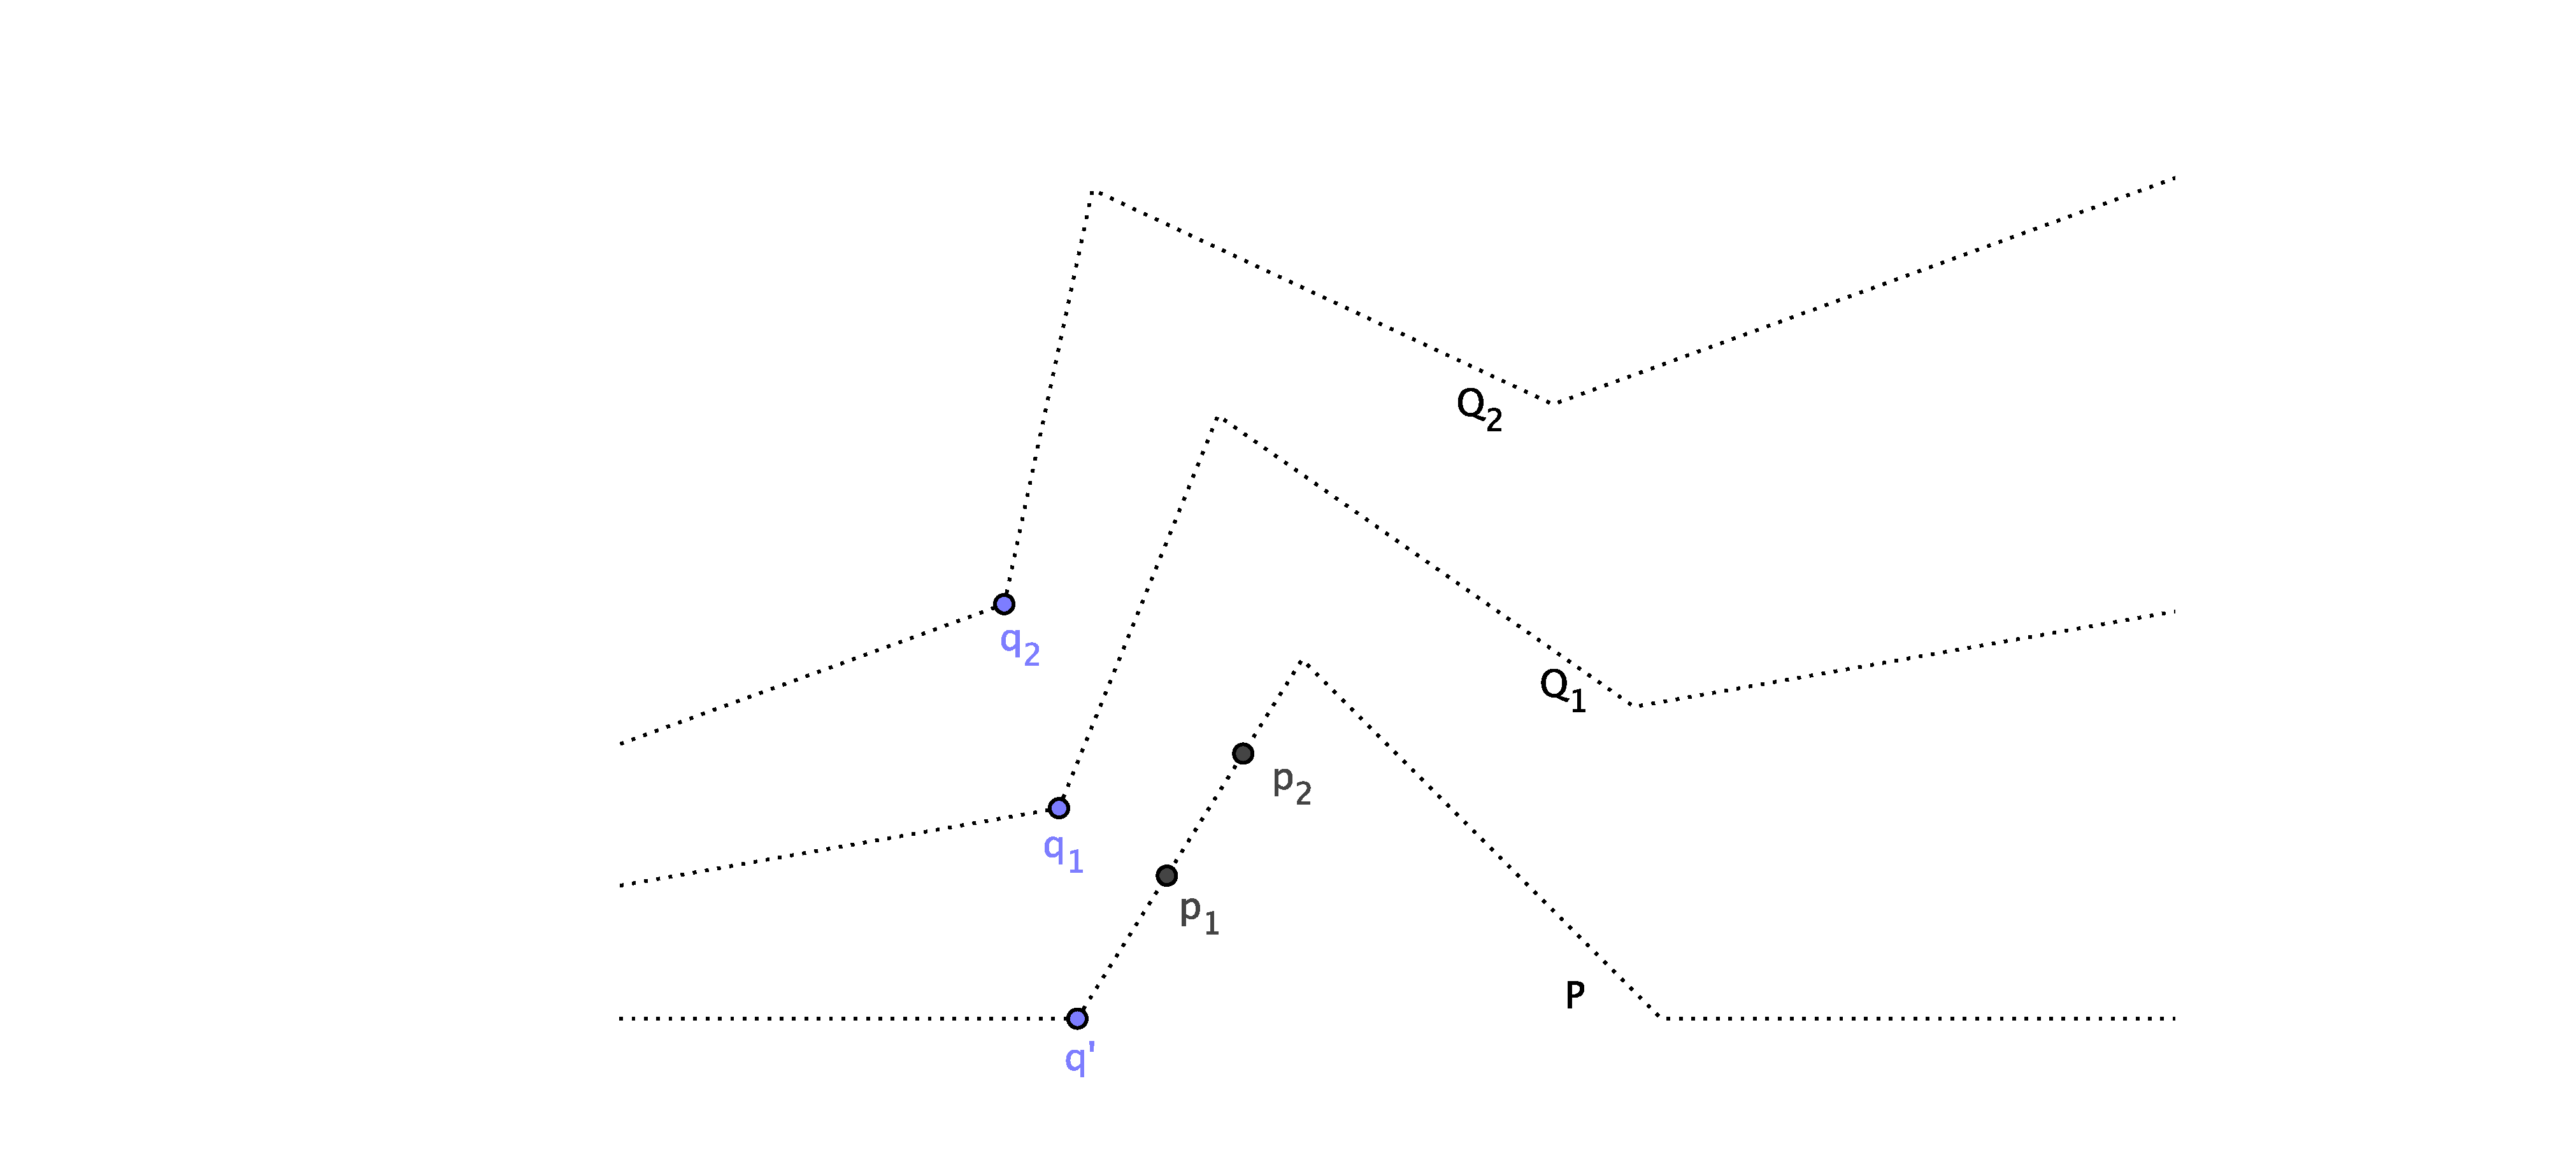
\includegraphics[width=.5\textwidth]{fig/icp_true_approx_cor.pdf}
\caption{Single point at two ICP iterations}
\label{fig:icp_true_approx_cor}
\end{wrapfigure}
The figure shows a fixed point cloud $P$, and a loose point cloud $Q$ at two different alignments, $Q_1$ being aligned more accurately than $Q_2$. $q_2, q_1, q'$ represent the same position in the coordinate systems of the three point clouds. $q \in Q$, but in general $q' \notin P$ except when $Q$ and $P$ have exactly the same constellation.
$p_1, p_2 \in P$ are the correspondence points chosen for $q_1$ and $q_2$ by the closest point criterion.

Hypothesis (1) translates into $d(q_1, q') < d(q_2, q') \Rightarrow d(p_1, q') < d(p_2, q')$. If the point clouds consisted only of the line $\bar{q' p_1}$ this would be true from the triangle similarity. Clearly $\lim_{q \rightarrow q'} d(p, q) = 0$. But the convergence is generally not monotonous. For example if $q$ were to come in from another angle, $p$ could oscillate between the closest points from the two segments adjacent to $q'$.

The error minimization step pulls all $q_i$ closer to $q_i$. Because $\{ p_i \}$ and $\{ q_i \}$ have different constellations, they cannot be made to coincide, but $d(p_i, q_i)$ will get smaller in the least squares sense. \footnote{If it were to get larger, then $\matr{I}$ would be a better transformation estimation than the one found by least squares minimization.} This shows that $d(q_1, p_2) < d(q_2, p_2)$. $p_1$ is the closest point to $q_1$ by the closest point criterion, meaning that $q_2$ cannot be closer. Hence $d(q_1, p_1) < d(q_1, p_2) < d(q_2, p_2)$. This proves the convergence of the ICP algorithm with the closest point criterion.

For hypothesis (2) to be satisfied, it must additionally be true that $d(q', p_1) < d(q', q_2)$. When this is not true, the algorithm can converge towards a local minimum.



\subsubsection{Local minima}
ICP minimizes an error function $e : \mathbb{R}^6 \rightarrow \mathbb{R}$ taking as input a rigid transformation, which can be represented using $6$ independent variables. The function $e$ is different at each iteration, and depends on the correspondences.


\subsection{Generalized ICP}
Conceptually, the difference between point-to-point ICP and point-to-plane ICP is that in the point-to-plane variant, the position of a point on a surface has no impact on the error metric and minimization. This is useful because the point clouds represent solid surfaces approximated using a discrete set of points, and the goal of a registration algorithm is to align those surfaces, and not the points that represent it. The registration algorithm should be agnostic to the distribution of points on a surface.

\emph{Generalized ICP}, first described in \cite{Sega2009}, is a generalization that covers both these variants. Each point is replaced by a gaussian probability distribution that models the uncertainty of its position on the surface and orthogonal to the surface. From this a new error metric formula to minimize is deduced that includes covariance matrices for the two points' distributions.


\section{Coarse Registration}
For coarse registration, no initial alignment of the point clouds is used, and the goal is to obtain an approximative alignment of matching point clouds, which can then be improved upon using fine registration. 

\subsection{Manual registration}
Most commonly, coarse registration is done manually. One method is to define at least three pairs of corresponding positions in the two point clouds, another to rotate and translate the point clouds using a 3D interface.

Both methods can be time consuming because one works using a two-dimensional projection of the two point clouds on a computer screen, the view is difficult to recognize when they incorrectly overlap, and one needs to be able to rotate and translate both the camera and the two point clouds. For these reasons automatic solutions can be preferred in practice, especially when the scanning project consists of many point clouds.

\chapter{Registration of Large Models}
The subject area of this paper is the registration of scans taken of a large and structurally complex physical objects. The thesis is set in the context of the full 3D scanning of the Brussels ``Hôtel de Ville'', a current project by LISA. In particular this paper focusses on the registration of long-range scans of the entire building with short-range, high resolution close-up scans of some features of it.


\section{``Hôtel de Ville'' scanning project}
This is a current 3D documentation projection by the the Image research unit of the \emph{Laboratories of Image, Signal processing and Acoustics} (LISA) at ULB. The goal is to create a full 3D model of the ``Hôtel de Ville de Bruxelles'' \footnote{Brussels Town Hall} building. It is a medieval building built in the beginning of the 15th century, with a Brabantine Gothic-style architecture.


\section{Relief point cloud}
As indicated in the beginning, the physical object is imagined as an ensemble of continuous two-dimensional surfaces embedded in three-dimensional space. The point cloud is taken to be a discrete set of points that lie on those surfaces. Because many different kinds of objects can be scanned and good approaches for processing and registering them vary depending on many factors, it is useful to restrict the scope to a particular kind of point cloud.

Therefore only point clouds that model a single, approximatively planar surface are considered. The defining characteristic is how well it can be represented as a height map on a plane $A_P$. Scans of engravings on a stone wall, such as the ``dessus-de-porte'' on figure \ref{fig:hdv_dessus} can for instance be put into this category. This type of surface will be called ``relief'' in this paper.

\subsection{def}
Let $A$ be a plane and $P$ a point cloud, both in the same coordinate system. For each $\vec{p} \in P$, $d(p)$ is the signed orthogonal distance from $\vec{p}$ to $A$, and $\vec{p_A}$ the projection of $\vec{p}$ onto $A$.


\subsection{Artificial relief} \label{sec:art_relief}
To be able to study registration of point clouds, it is useful to generate artificial points clouds that fit into this category and for which exact values of the underlying surface can be computed.

An algorithm was devised to generate artificial relief surfaces, which look as shown on figure \ref{fig:relief_render}.

\begin{figure}[H]
\centering
\begin{subfigure}{.5\textwidth}
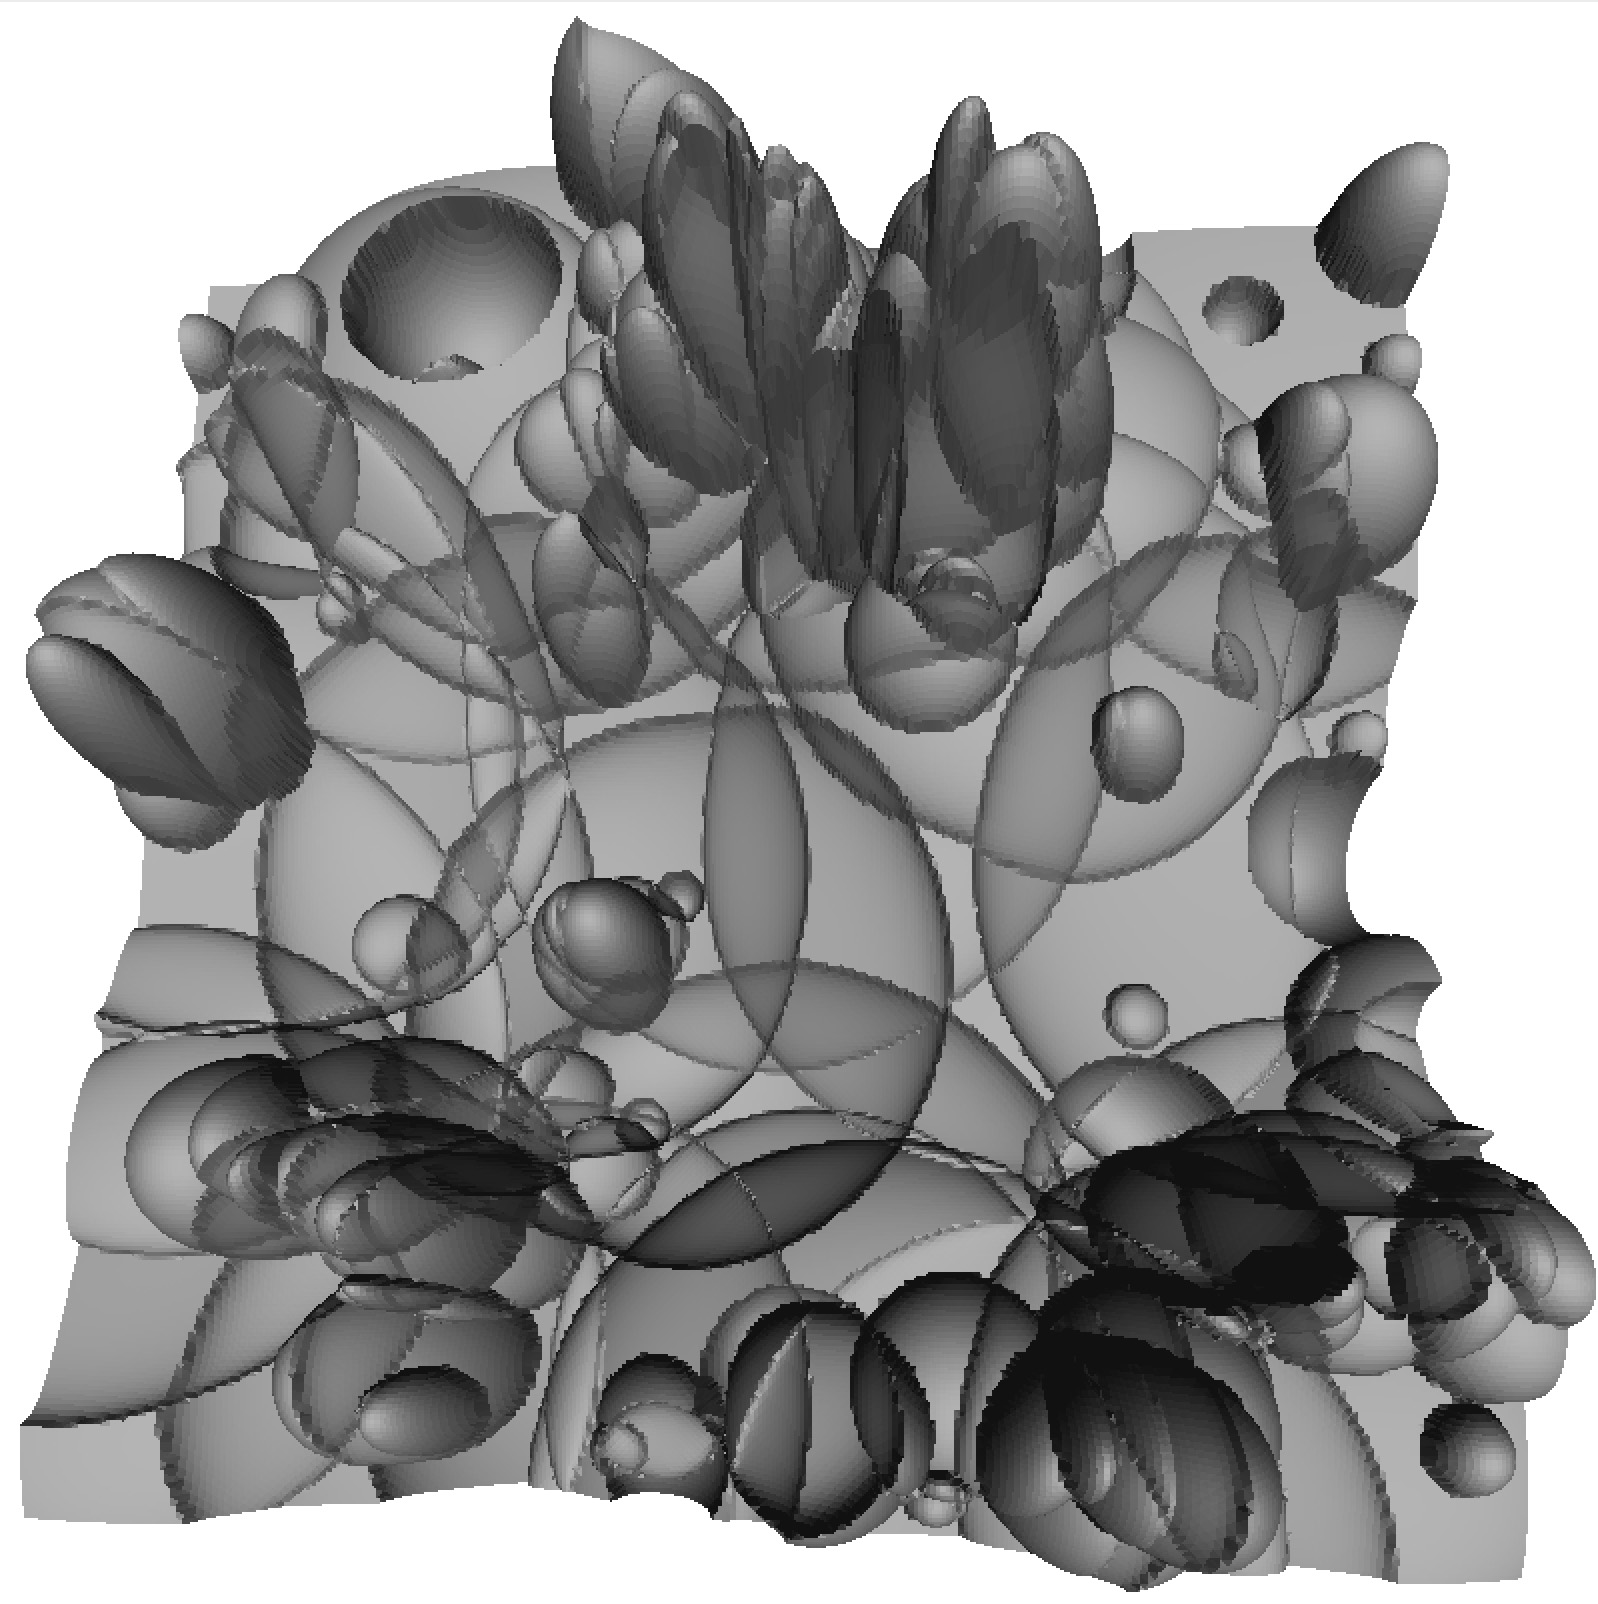
\includegraphics[width=\linewidth]{fig/r1_render2.jpg}
\end{subfigure}%
\begin{subfigure}{.5\textwidth}
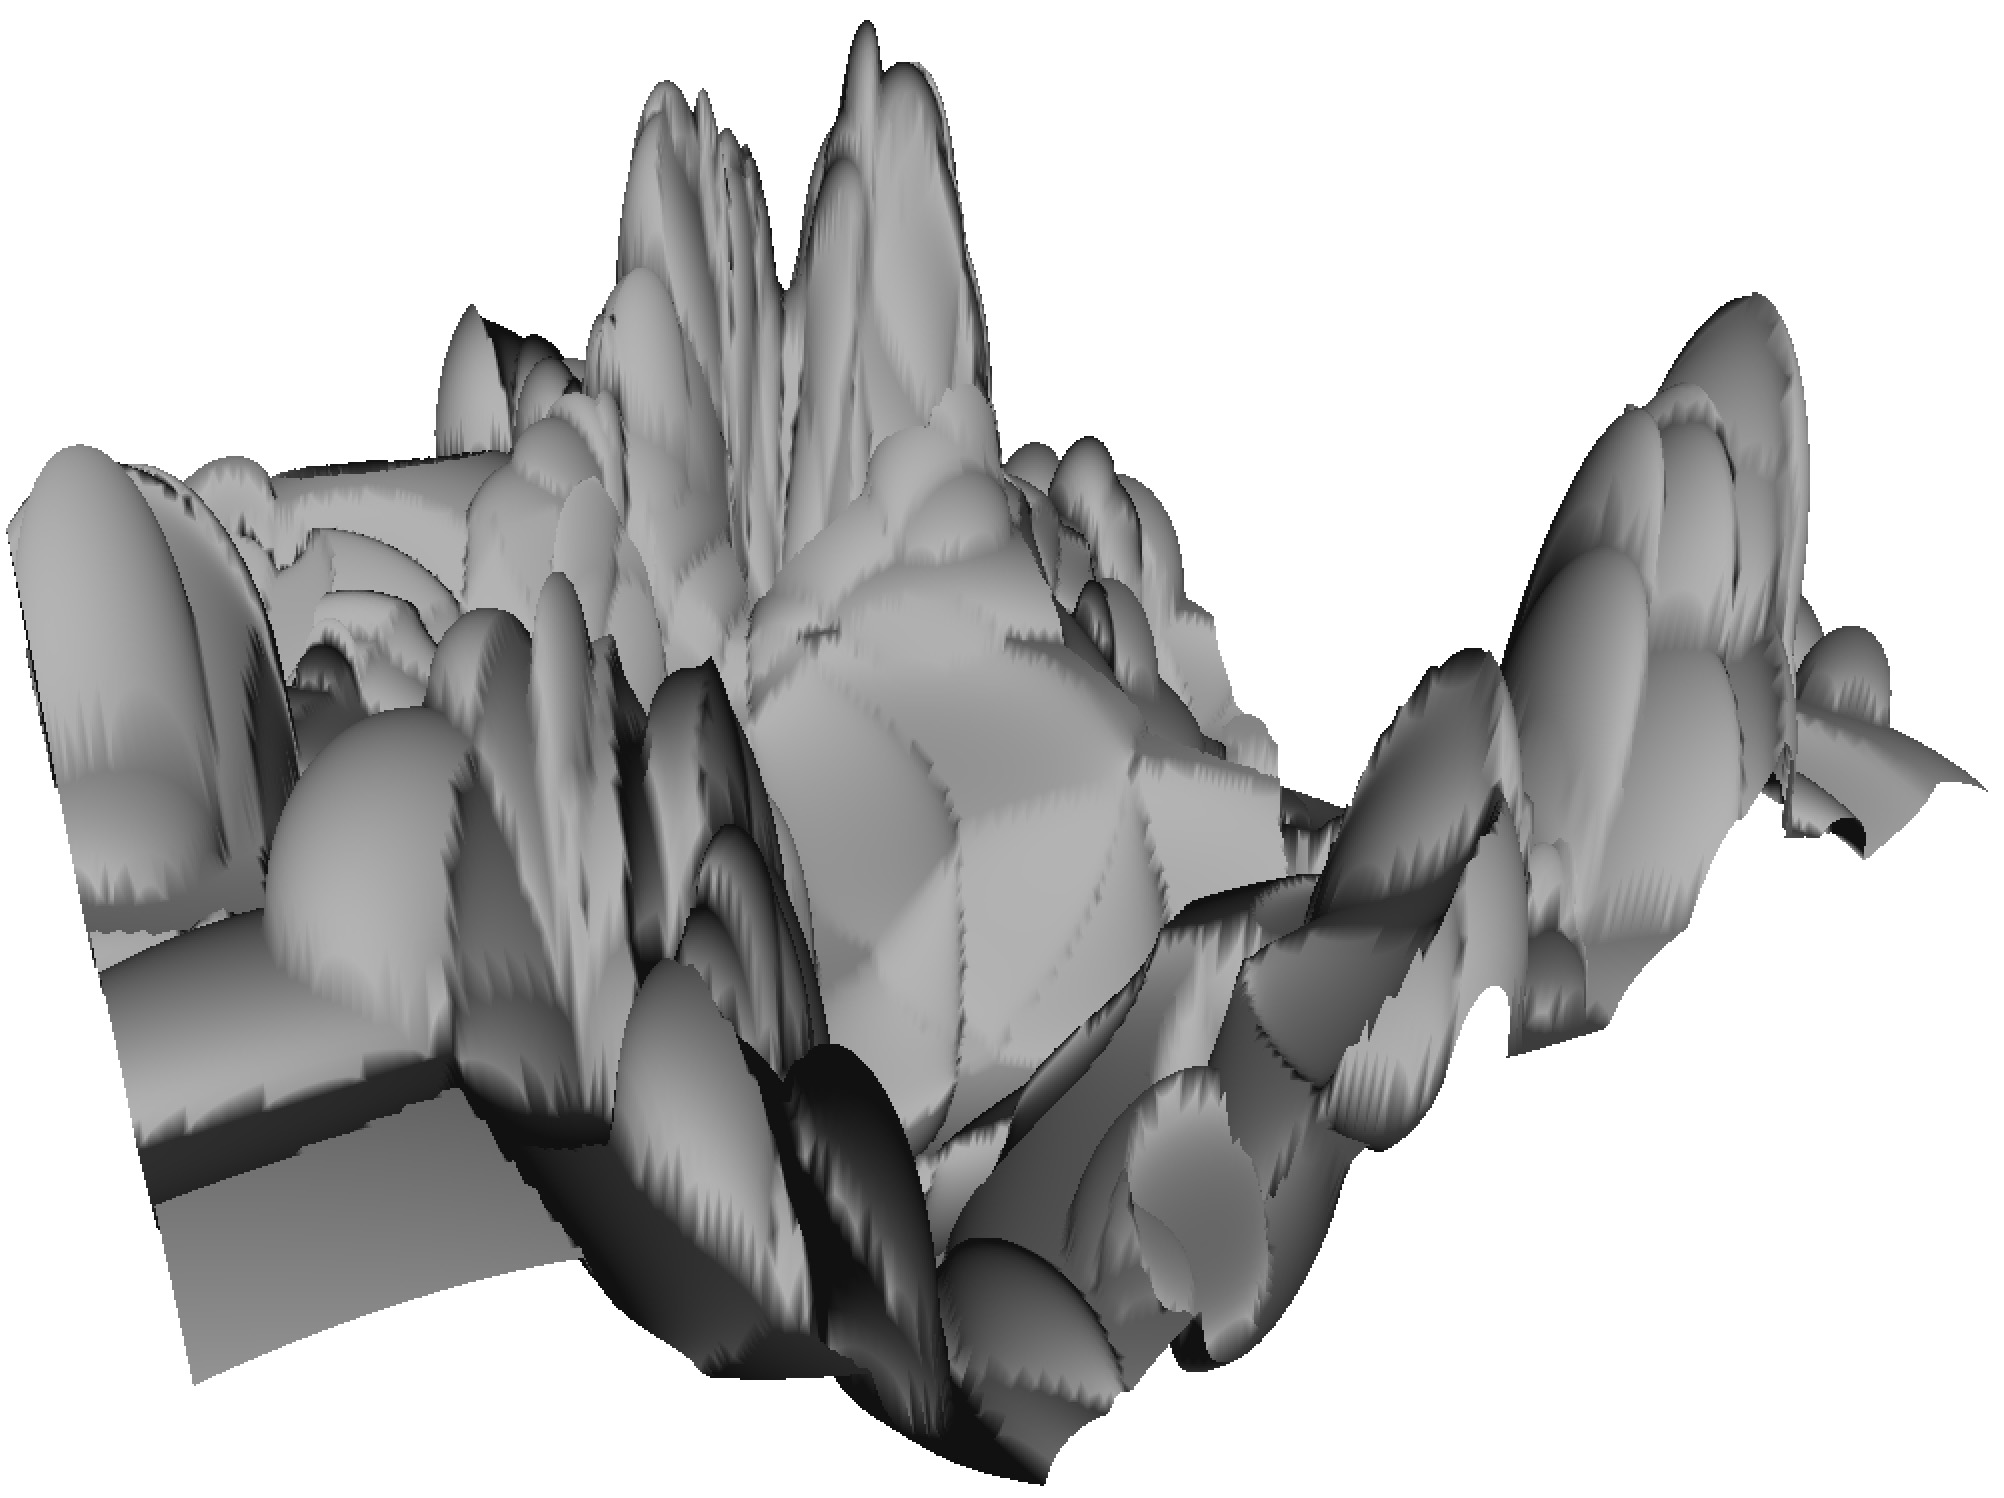
\includegraphics[width=\linewidth]{fig/r1_render1.jpg}
\end{subfigure}
\caption{Artificial relief surface, seen from two view points}
\label{fig:relief_render}
\end{figure}

The entire algorithm is randomized, but can be made deterministic by specifying a seed value for the random number generator. The surface to generate is specified by a \emph{width} $w$, a \emph{height multiplier} $h$, and this seed value.

The generated point cloud is a height map on the XY-plane. Let $z = R[x,y]$ be the $z$ component of the single point with given $x, y$ components. It is defined for $-\frac{w}{2} \leq x,y \leq +\frac{w}{2}$. At first, let $R[x,y] = 0$ for all these points. The result is a square surface of side length $w$.

The algorithm proceeds by pushing randomized ``embossings'' into the surface. The embossings are the shape of a half-sphere distorted in one direction, and is described using the height map formula
\begin{equation}
B_i[x,y] = \pm \, h_i \sqrt{1 - \frac{(x_i - x)^2 + (y_i - y)^2}{r_i^2}}
\end{equation}
A plot of its two-dimensional analogue is shown in figure \ref{fig:relief_B}. $B_i[x,y]$ is set to $0$ for coordinates $x,y$ outside its domain, that is, for $x,y : (x_i - x)^2 + (y_i - y)^2 > r^2$. As a consequence a sharp circular corner is formed around the border.

A fixed number $n$ of embossings are generated with different parameters, and are added to $R$, so that
\begin{equation}
R[x,y] = \sum_{i=1}{n} B_i[x,y]
\end{equation}

The resulting height map will be split into regions $\{(x,y)\}$ where different subsets of $\{B_i\}$ are active. ($B_i$ is active when $(x,y)$ lies in its domain). $R$ has sharp corners at the border points of all $B_i$. As soon as more than one embossing is active in one region, the $z$ coordinate becomes a sum of square roots, producing a complicated shape for both the continuous surface areas and the corners. Its partial derivatives can still easily be calculated analytically, which allows for accurate computation of normal vectors. 

\begin{figure}[h]
\centering
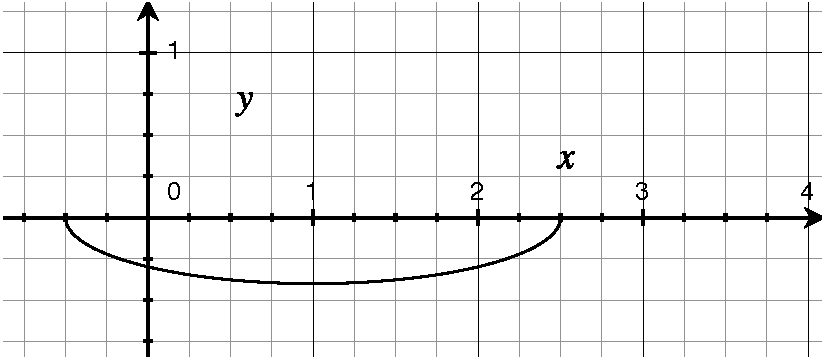
\includegraphics[width=.5\textwidth]{fig/relief_B.pdf}
\caption{2D example for relief embossing, with $h_i = -0.4$, $r_i = 1.5$, and $x_i = 1.0$}
\label{fig:relief_B}
\end{figure}

The radius $r_i$, height $h_i$ and center $(x_i, y_i)$ are randomly chosen for each embossing $B_i$. $x_i, y_i$ are chosen with a uniform distribution in $[-\frac{w}{2}, +\frac{w}{2}]$. The parameters for choosing $r_i$ and $h_i$ are set in such a way that the resulting surface will contain both flat regions and ``spikes'', which occlude parts of the surface when viewed from the side. $h_i$ can be both positive or negative.

\subsection{Point cloud generation}
\subsubsection{Top-down view}
Two ways of generating a point cloud of a relief surface are used. The simplest way is to simply take a set of points $\{ x, y, R[x,y] \}$. It results in a \emph{top-down} view of the surface, as seen by an orthogonal projective camera looking in $-z$ direction. From that view point the model has no occluded surfaces. The $x, y$ coordinates are arranged on a square grid, with a given density $\rho$. Figure \ref{fig:relief_plain} shows an example of such a point cloud, itself projected with a perspective camera.

\begin{figure}[p]
\centering
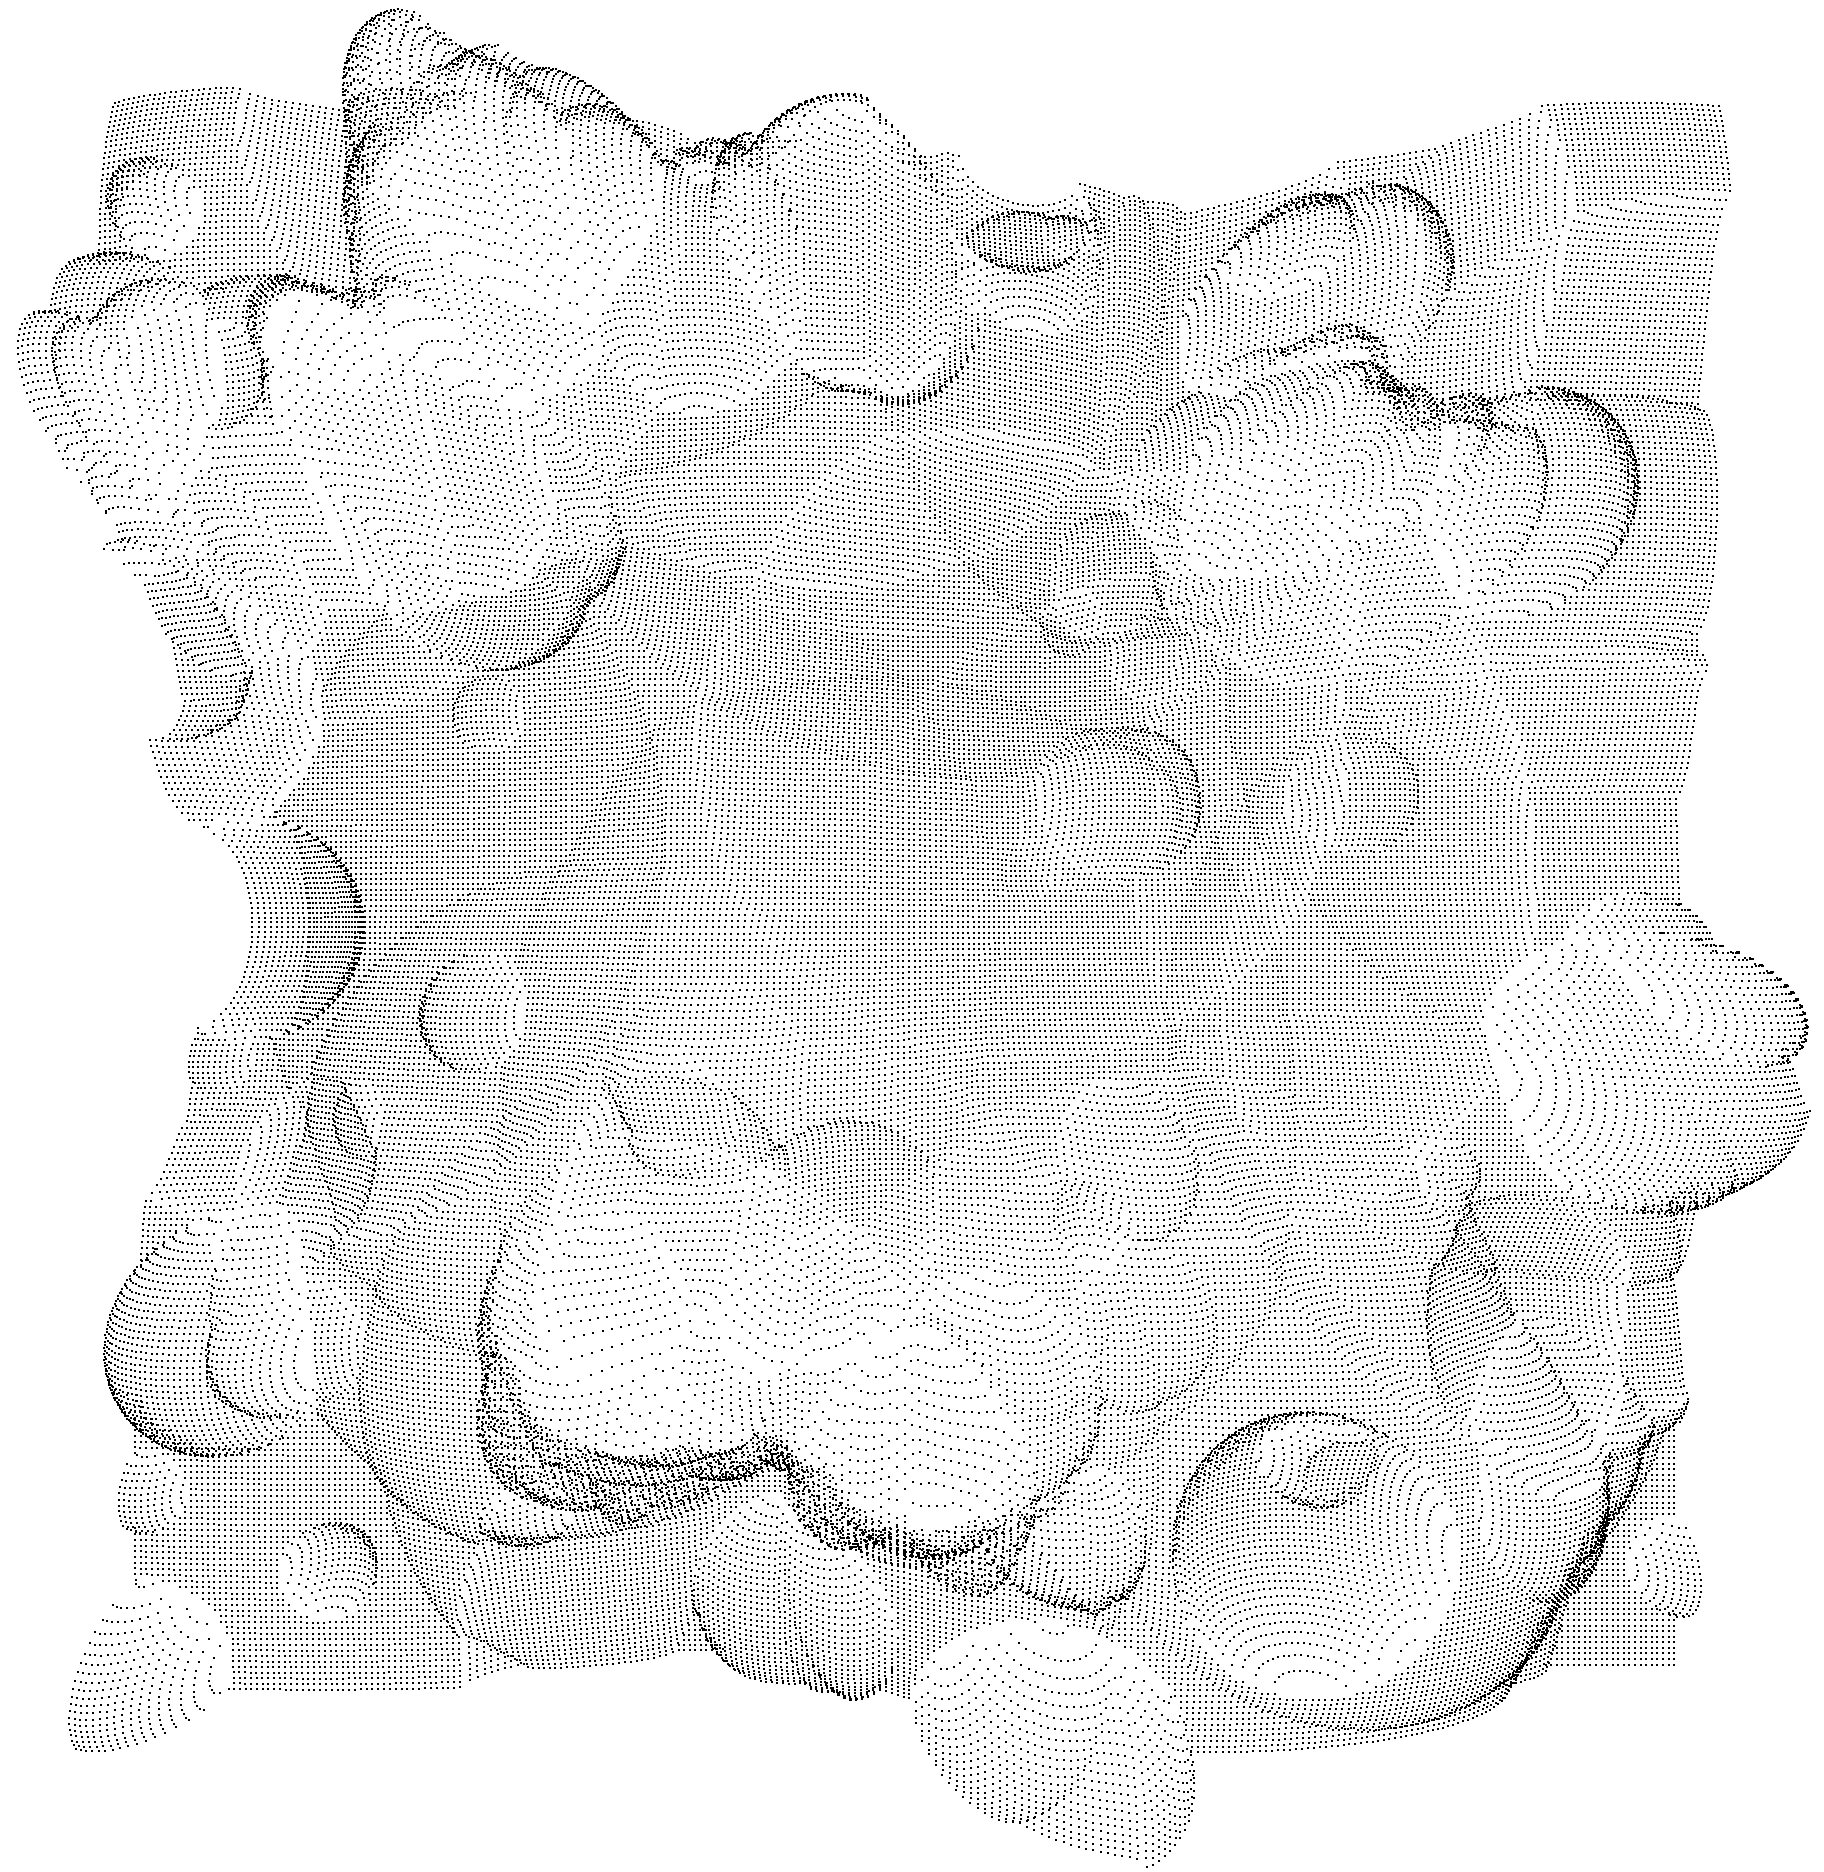
\includegraphics[width=\textwidth]{fig/r1_plain.png}
\caption{Top-down point cloud of relief}
\label{fig:relief_plain}
\end{figure}

\subsubsection{Occluded view}
However the goal of the artificial relief surface was to simulate the kinds of surfaces that occur on real objects, and to get a point cloud with similar properties to a 3D scan of it. So it is important to be able to generate point clouds of the relief as seen from another camera positions, with the occlusions that occur.

A virtual camera is placed near the surface at a given pose, and a range image is generated using it. With an orthogonal projection camera, the point density on the surfaces will remain constant, and with a perspective projection camera, it will decline with distance to the camera.

For the algorithm that creates this range image, a first attempt was to first generate a top-down view point cloud with high enough density, and then generate project that point cloud into a range image as described in \ref{sec:pc_registration}. However, this inevitably leaves points in the occluded areas.

Another attempt was to implement a ray-tracing method that operates on the expression of $R[x,y]$: For each image pixel, calculate the intersections with the view ray and the surface $R$ and take the closest one. However, these intersections cannot easily be calculated analytically. Firstly, the various regions of $R$ with different active embossings must be considered separately. But even on a single such region, multiple intersection points can still occur, and there is no direct closed-form expression for finding them. So a lot of combinatorics and numerical approximation would be required.

Instead, the implemented algorithm generates a mesh of the surface, projects a depth map of it onto image space, and then back-projects the image pixel coordinates into points. Figure \ref{fig:relief_occlusion} shows the resulting point cloud from two view points, the second one near the projection camera pose.

\begin{figure}[h]
\centering
\begin{subfigure}{.5\textwidth}
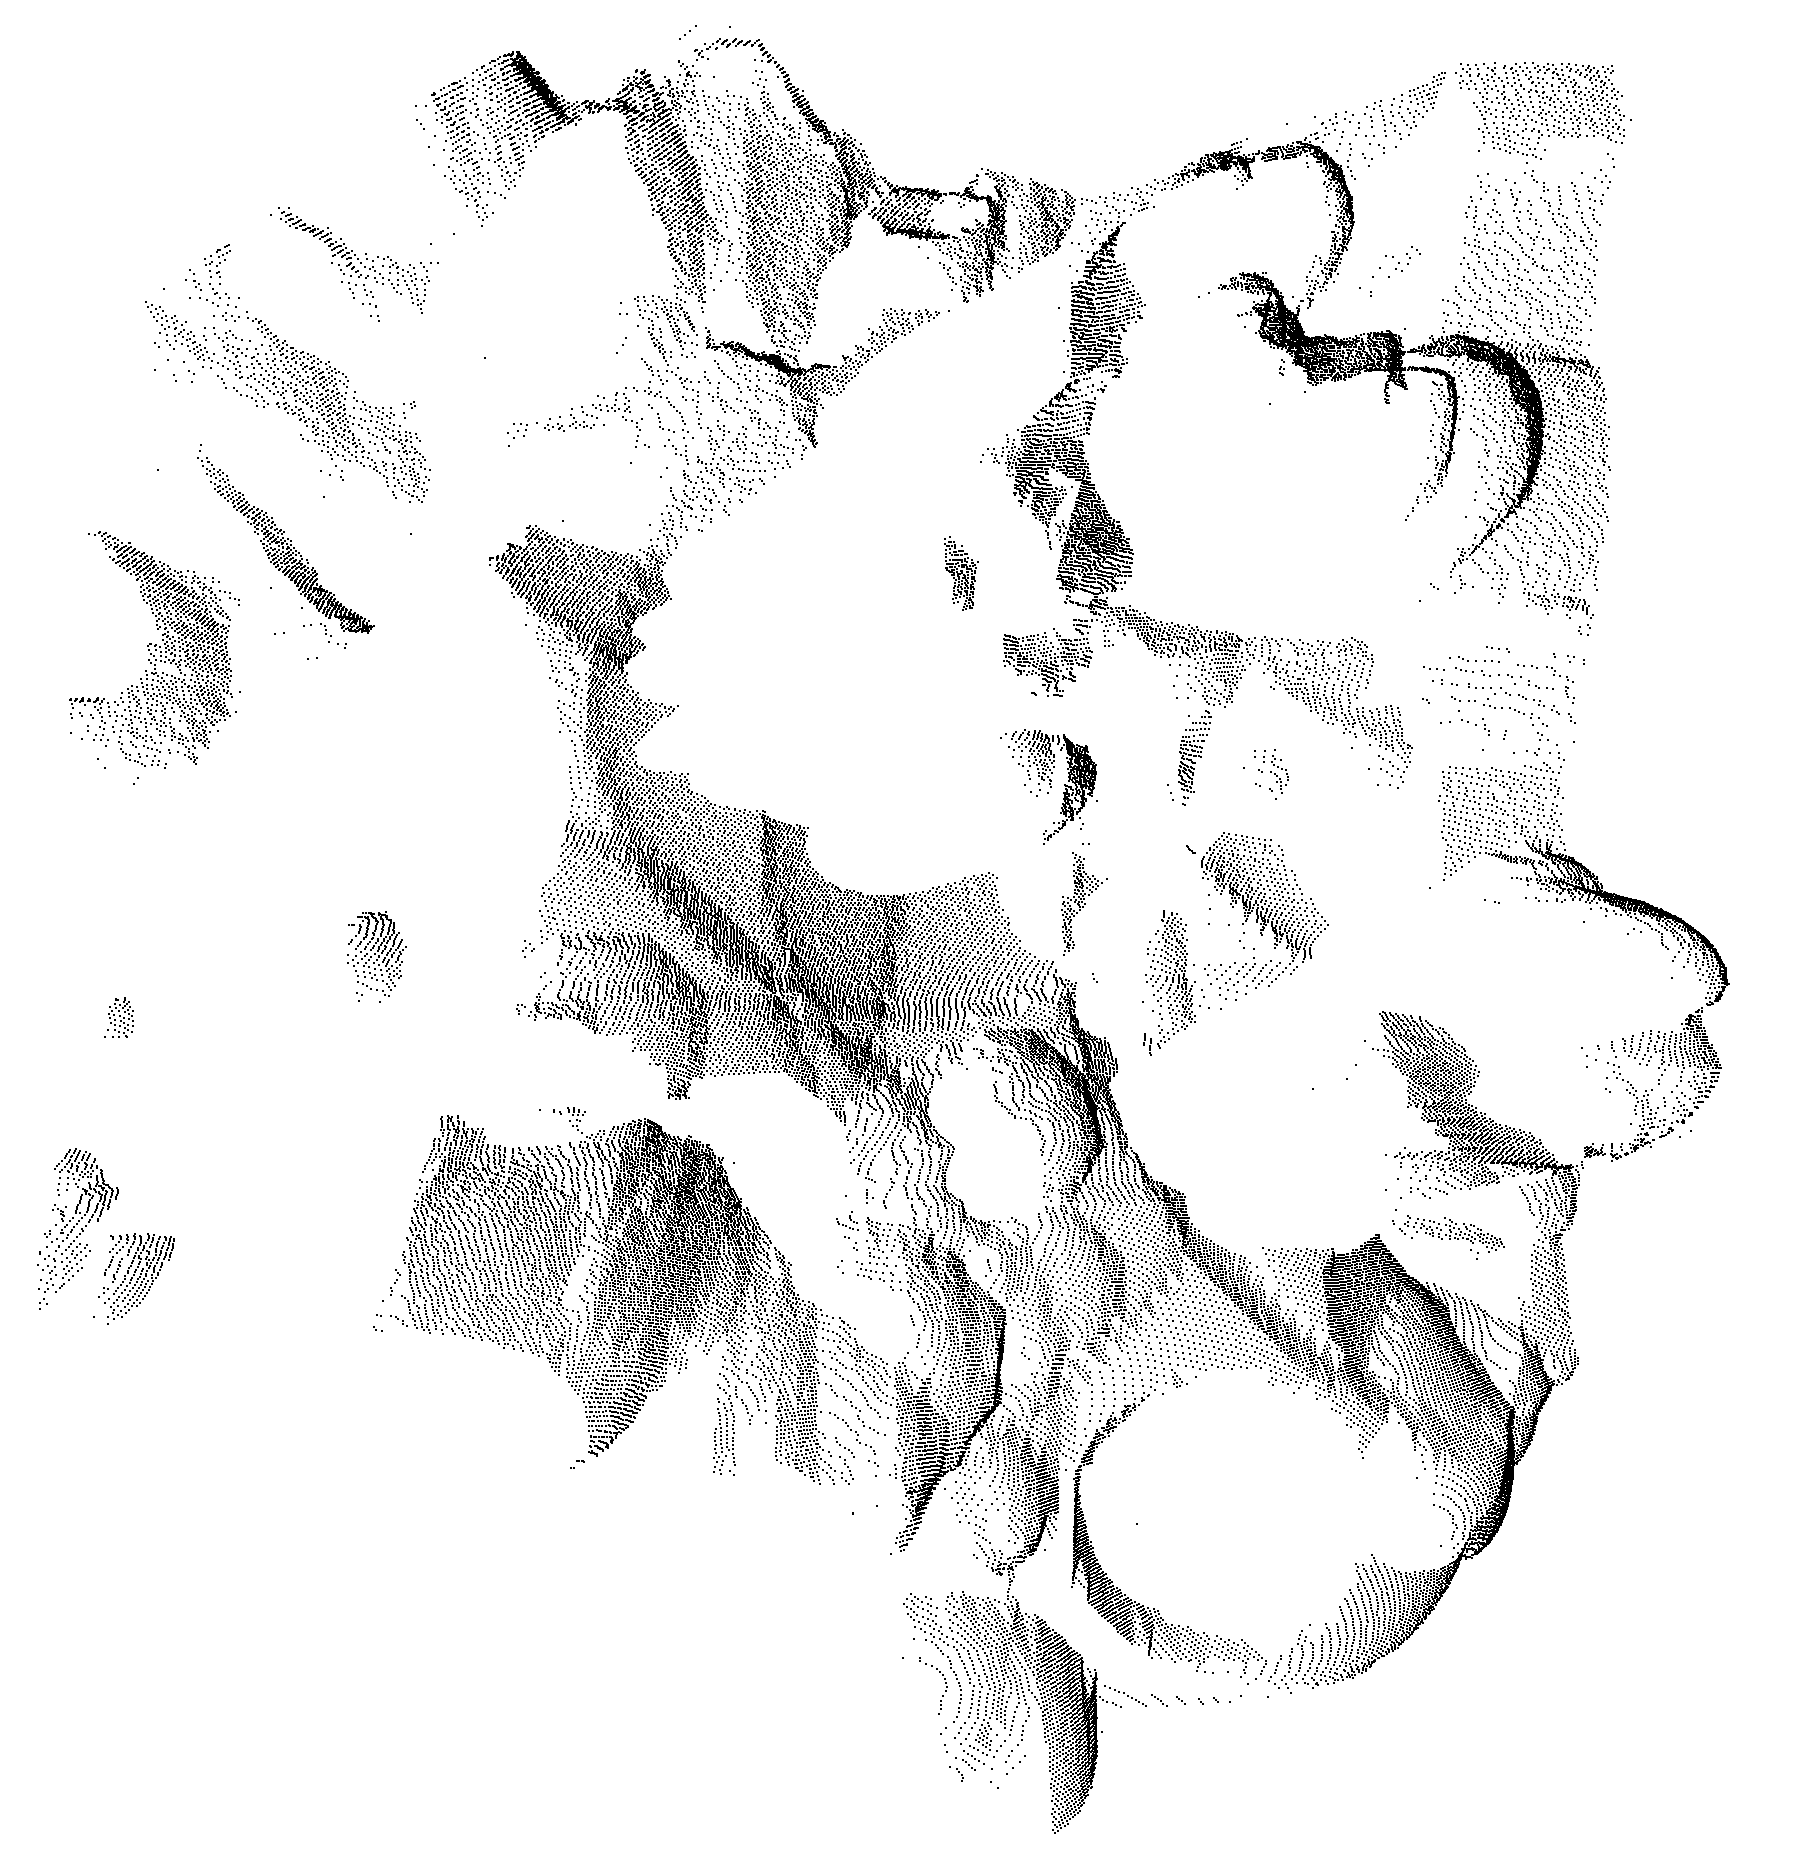
\includegraphics[width=\linewidth]{fig/r1_occlusion.png}
\end{subfigure}%
\begin{subfigure}{.5\textwidth}
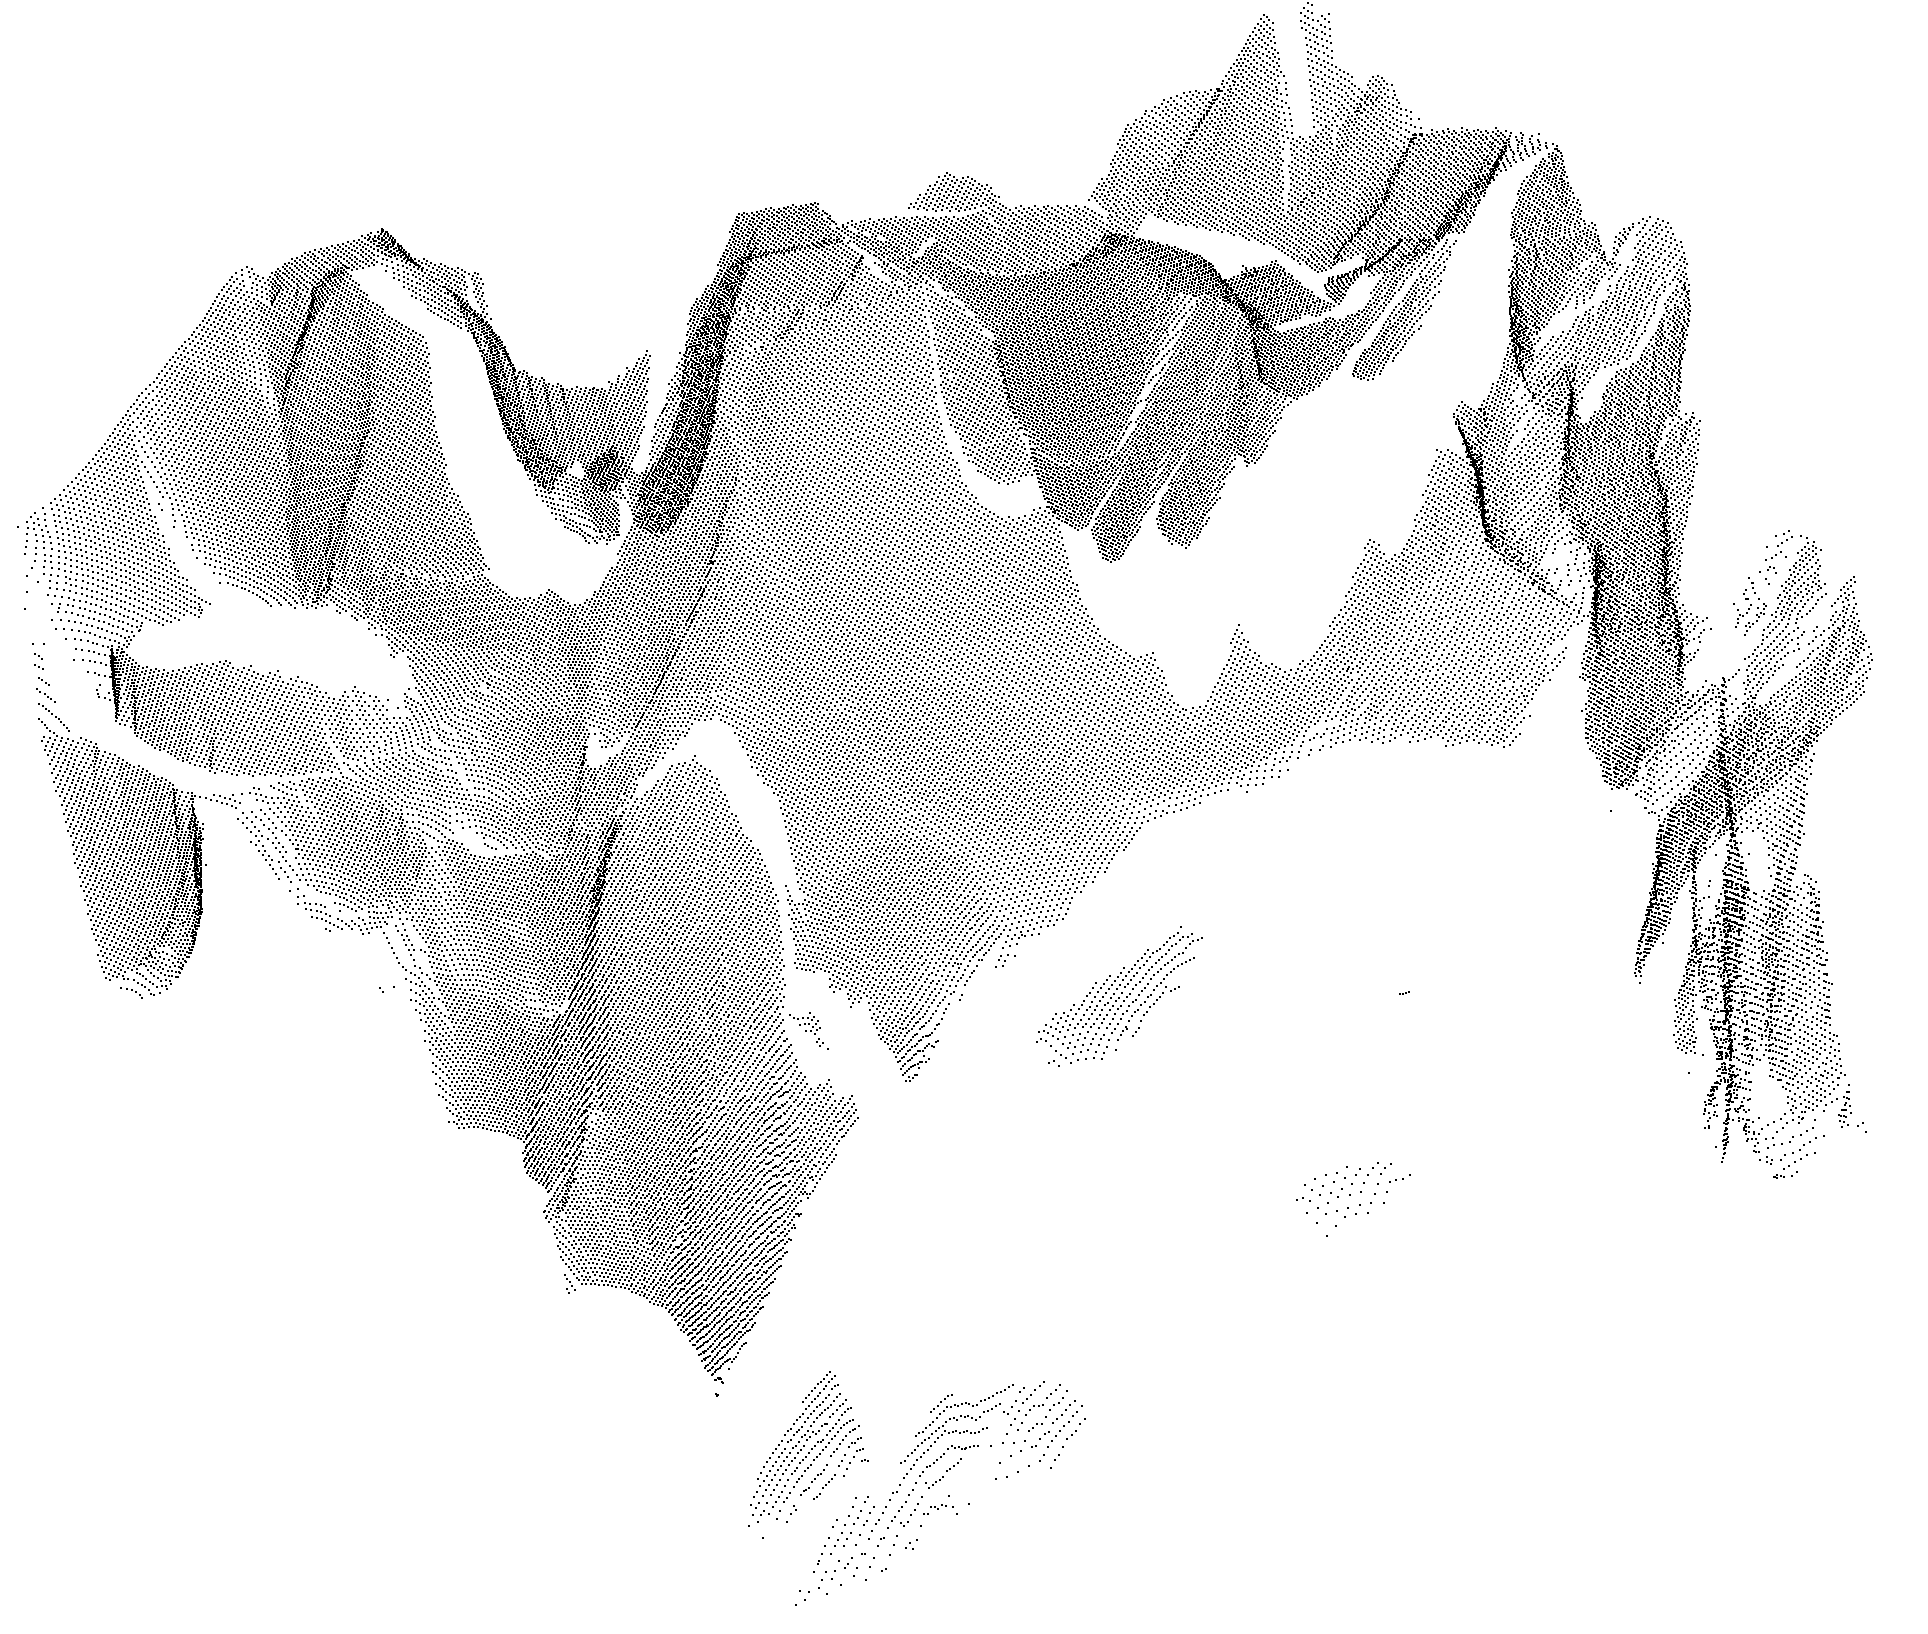
\includegraphics[width=\linewidth]{fig/r1_occlusion2.png}
\end{subfigure}
\caption{Artificial relief surface point cloud with occlusion}
\label{fig:relief_occlusion}
\end{figure}

A triangle mesh is generated by taking points $\{ x, y, R[x,y] \}$ with the $(x,y)$ coordinates forming a square grid of a given density $\rho$, and adding a diagonal edge into each square, in alternating direction. The number of squares per side must be even for this. As can be seen on the renderings in figure \ref{fig:relief_render}, this mesh does not handle the sharp corners well, but it is sufficient as errors are rectified in a later step.

For each triangle, its three vertices are projected into image space, using the given projection camera. This image is a Z-buffer contains, for each pixel, the inverted projected depth of the point\footnote{Z coordinate after application of camera projection matrix.}.

The width and height of this image space is set higher than that of the range image by a factor of about $k = 10$. Now each triangle is filled using a 2D rasterization algorithm. For each pixel, the inverted projected depths of the three corner points are linearly interpolated by using barycentric coordinates. This results in the inverted projected depth of the corresponding 3D surface point.

The actual occlusion culling is now done using a depth test: A pixel value is overwritten only if the inverse depth is higher than the previous one. This is the case only if the point is closer to the camera.

Each $k \times k$ square on this image corresponds to a pixel of the final range image. The center pixel is taken. Given $(x_i, y_i)$ in image space, and the inverse projected depth of the surface point, the 3D coordinates $(x, y, z)$ of the surface points can now be calculated.

Due to the limited accuracy of the mesh, and floating point precision problems, there is some error in this result. It can be rectified by recalculating $z' = R[x, y]$.

\subsubsection{Similarity with actual scans}
Figure \ref{fig:relief_crop} (called $R$) shows an artificial relief point cloud with occluded view and additionally cropped to a random polygonal region inside the original square. It is superimposed on a top-down point cloud of the same relief.

Figure \ref{fig:r1_ddp} (called $D$) is the high-resolution scan of the ``dessus-de-porte'', with colors removed.

The two point clouds are similar these some ways:
\begin{itemize}
\item Approximatively planar. For $R$ the plane is the XY-plane, for $D$ it is the stone surface behind the five statues.
\item Seen from a side angle and partially occluded.
\item Contain both smooth surfaces and sharp corners.
\item Points dispersed on a grid, as a result of the scan-lines, or of the image space in the virtual projection camera.
\end{itemize}

The important difference it that the underlying surface behind $R$ is known. The goal will be to develop a registration method that works for both $R$ and $D$ because of these common characteristics. With $R$ it can be tested both with and without knowledge of the surface.

\begin{figure}[p]
\centering
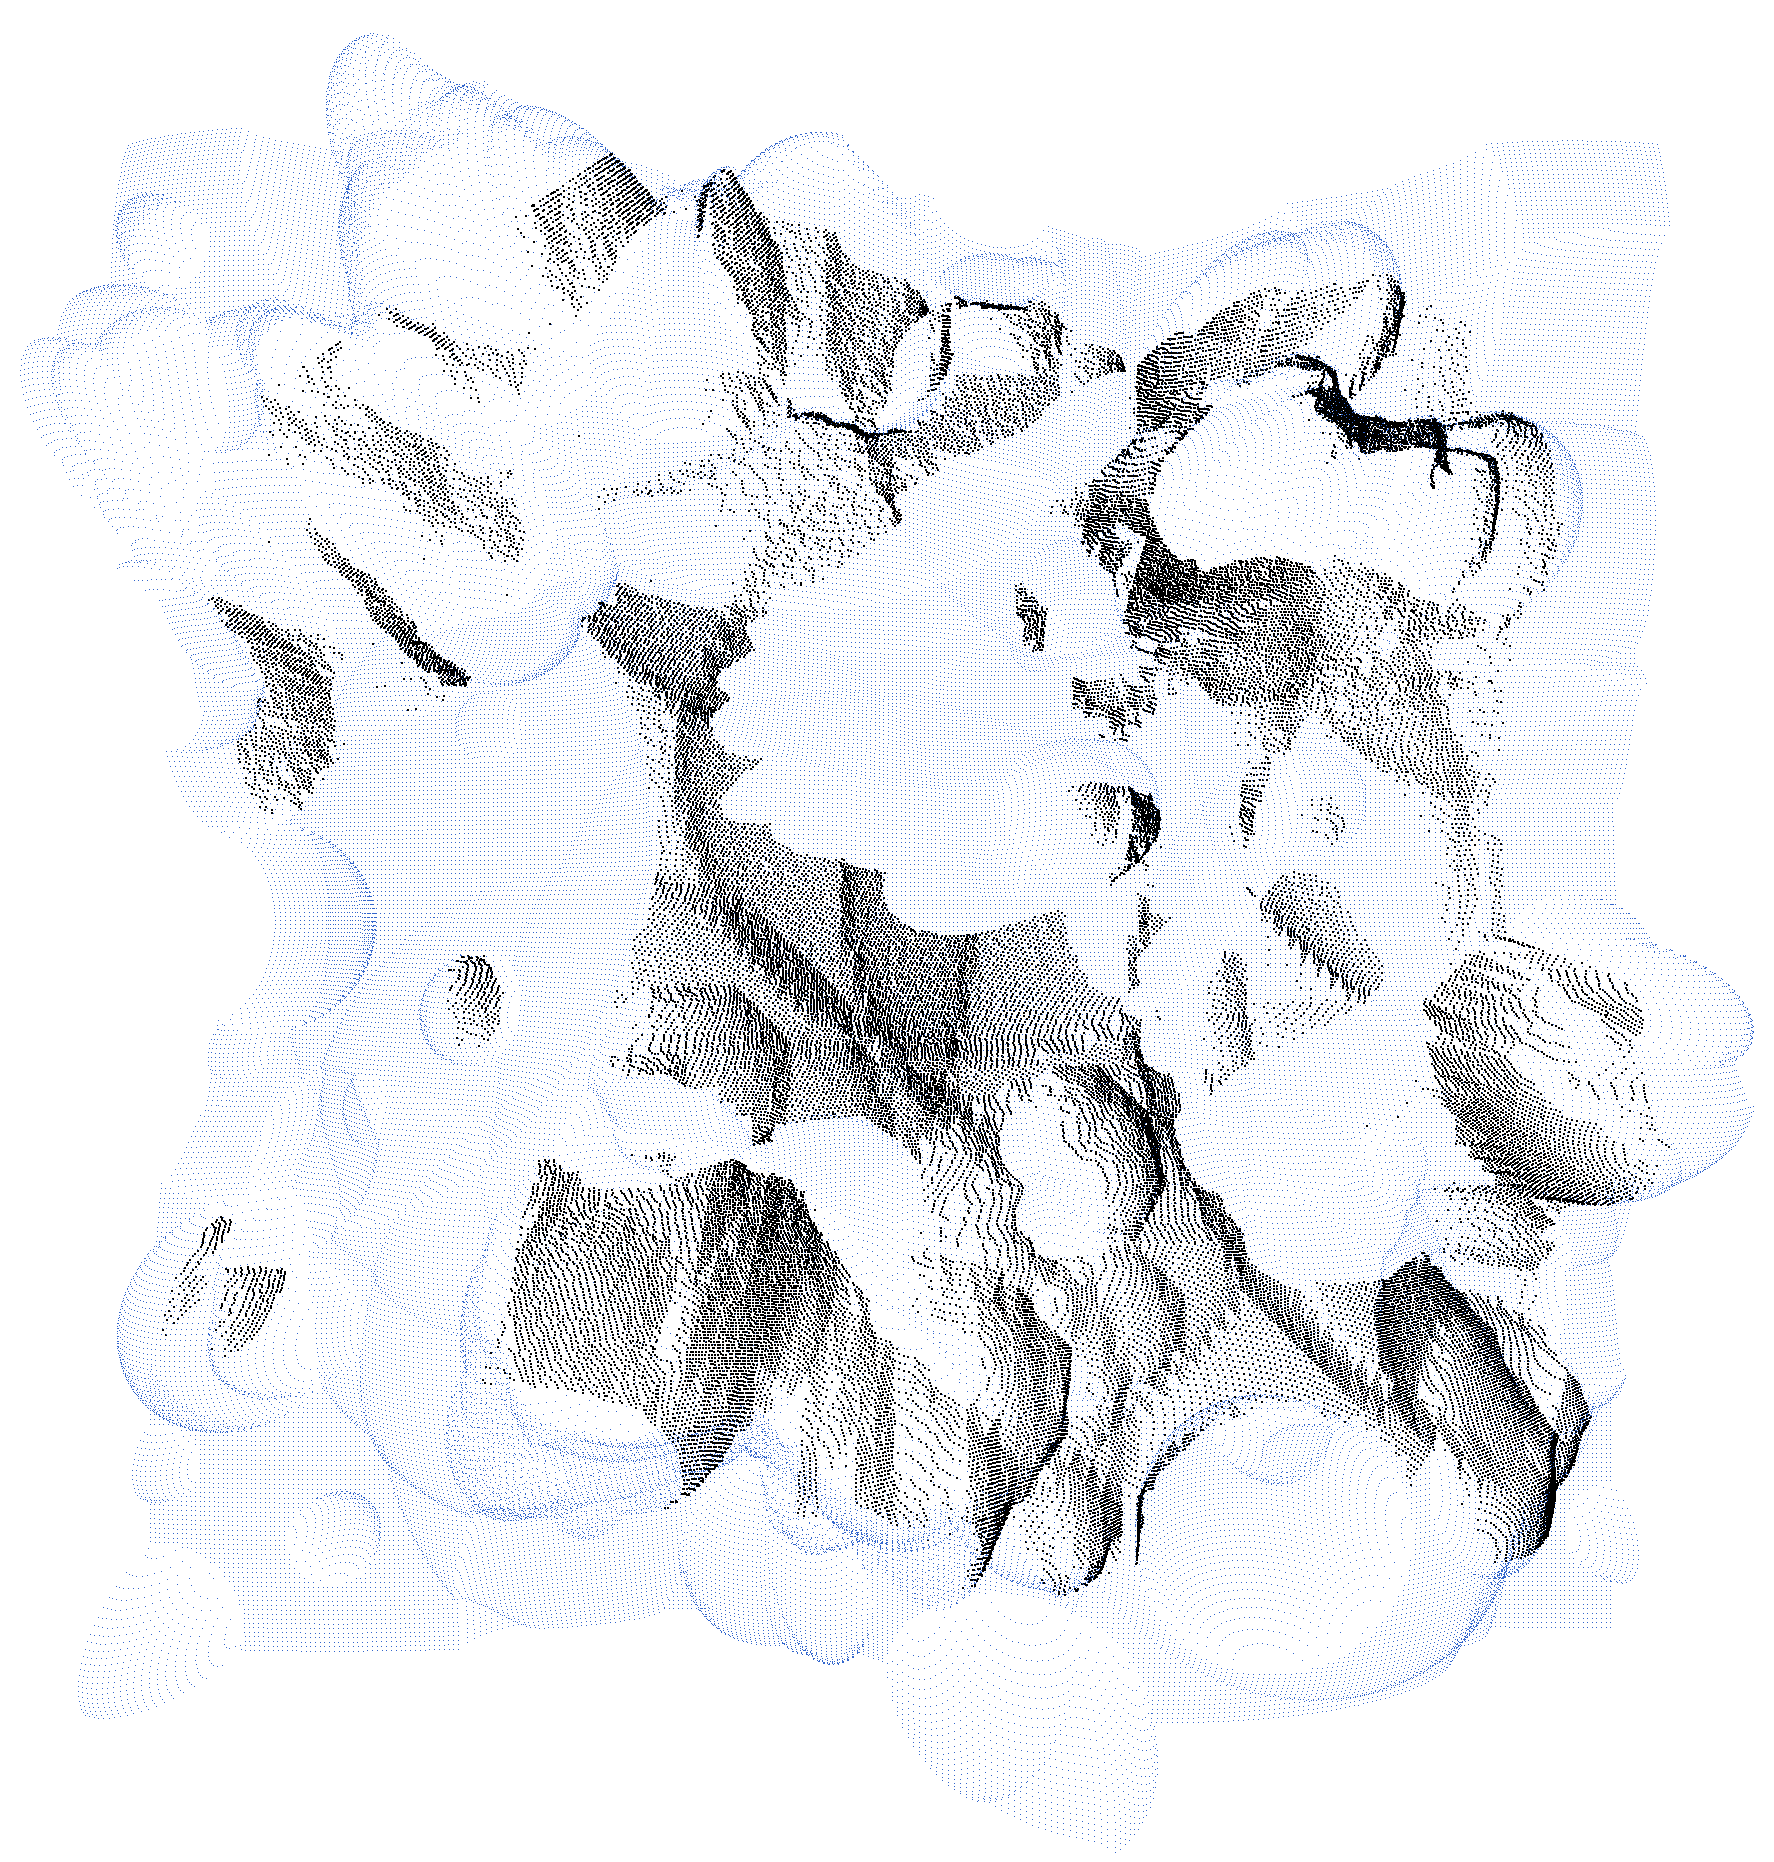
\includegraphics[width=0.7\textwidth]{fig/r1_crop.png}
\caption{$R$: Occluded view point cloud, and top-down point cloud of relief}
\label{fig:relief_crop}
\end{figure}


\begin{figure}[p]
\centering
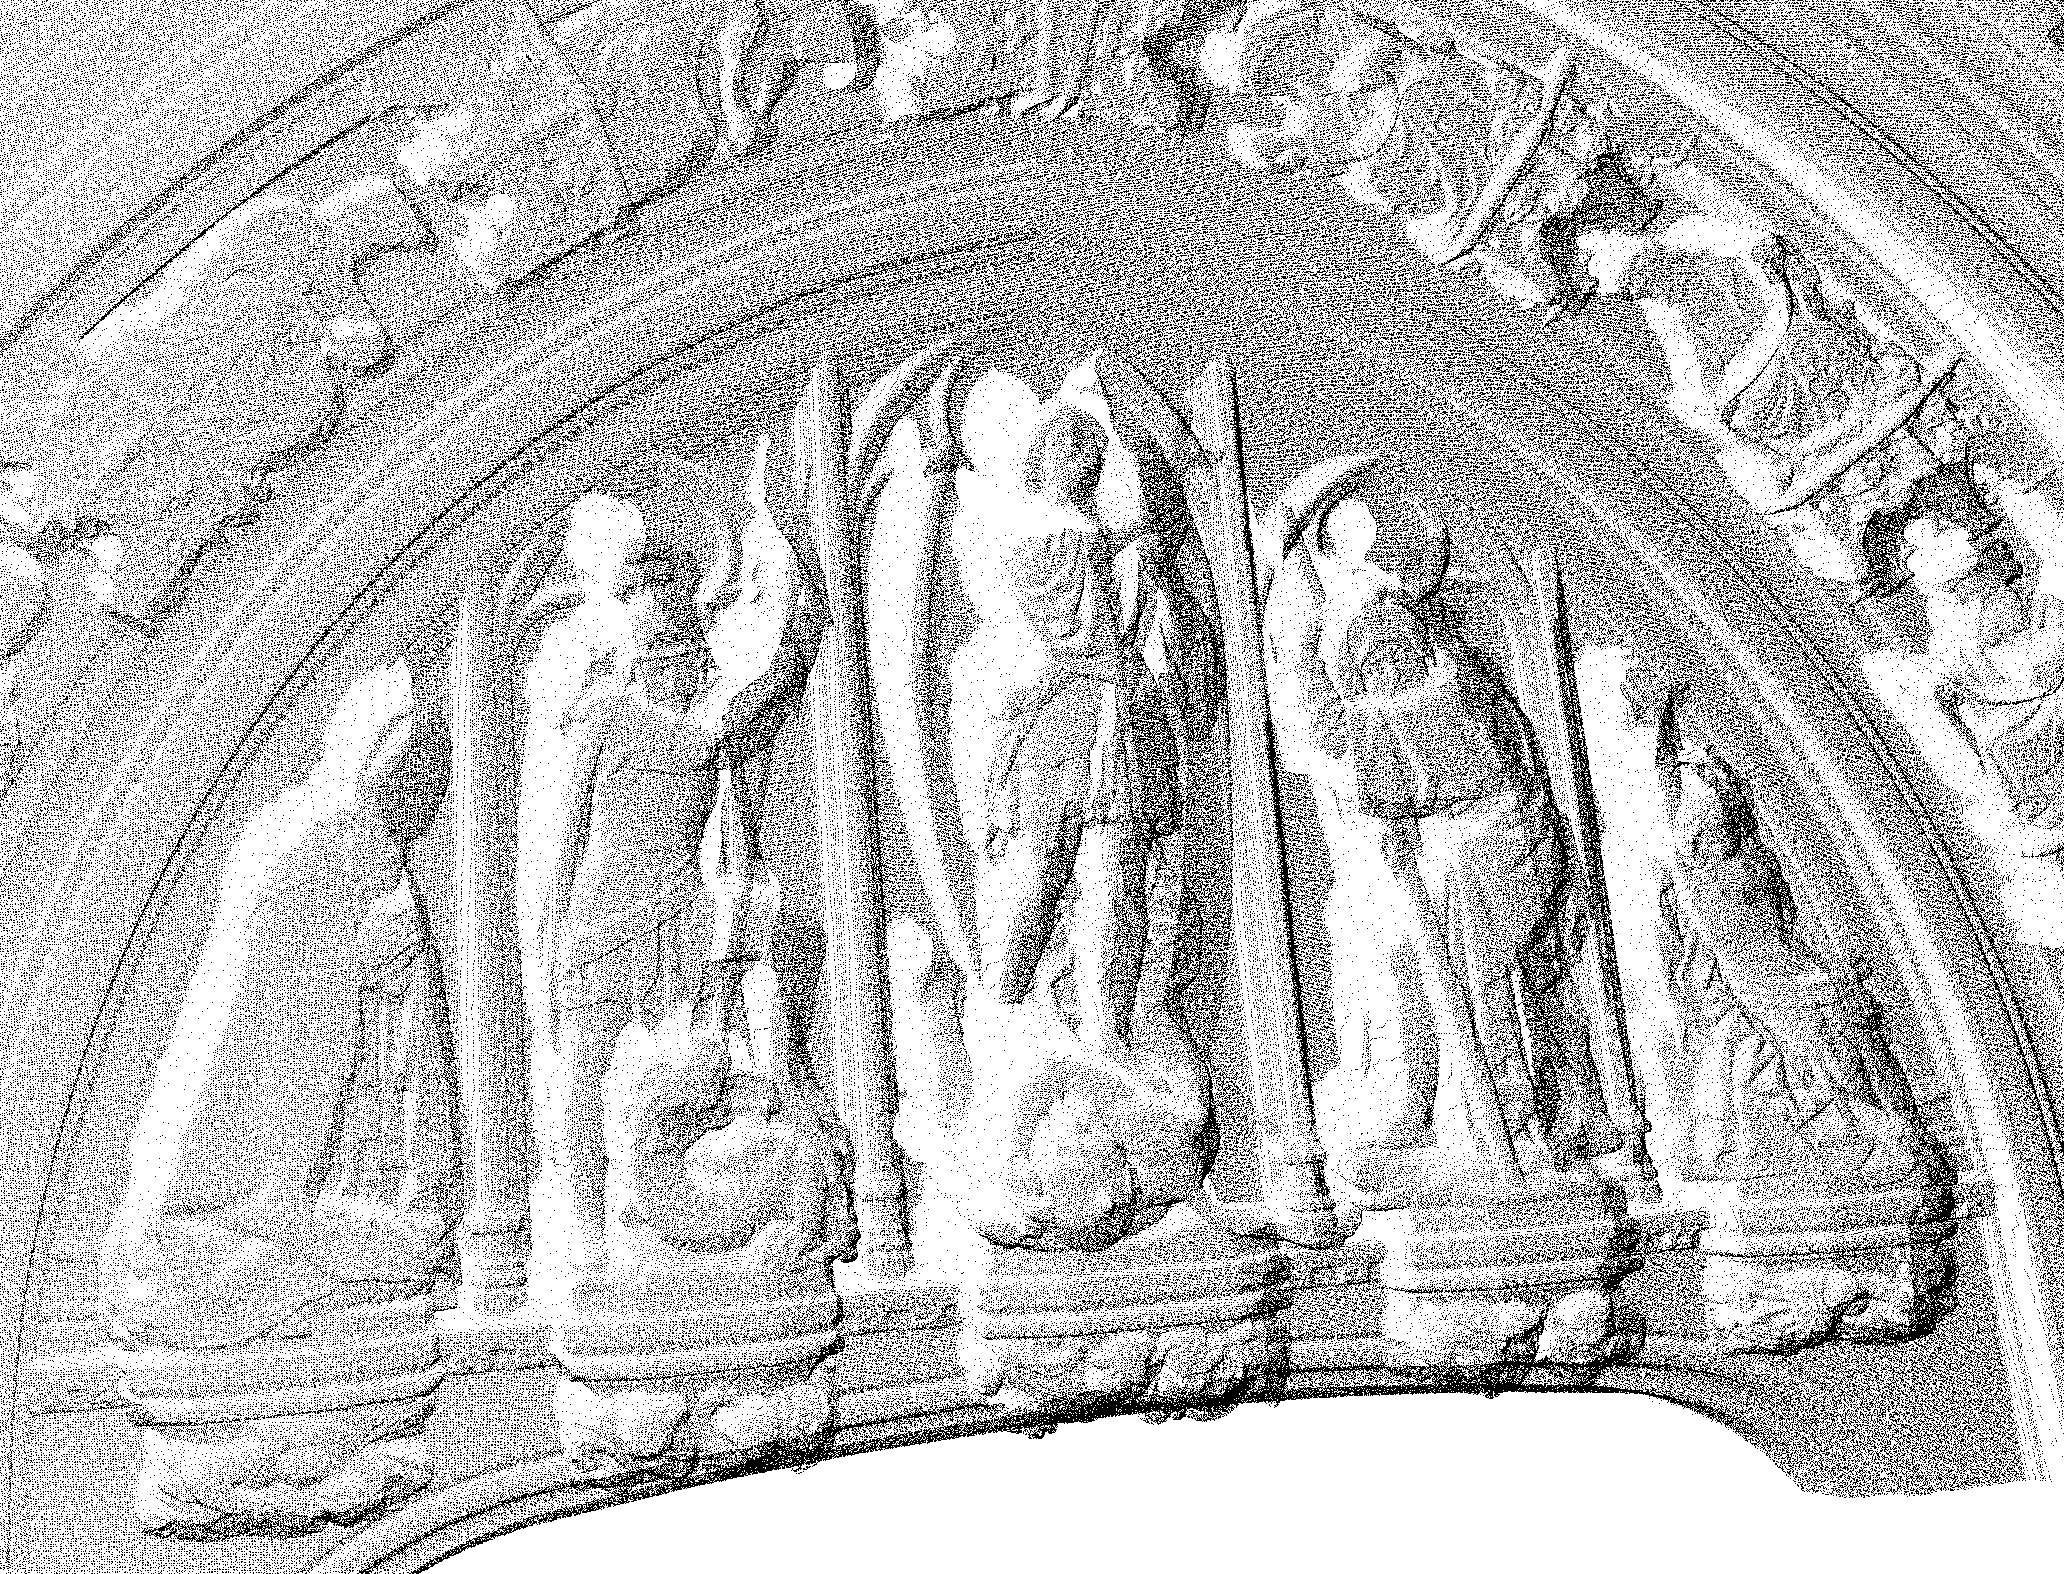
\includegraphics[width=0.7\textwidth]{fig/r1_ddp.png}
\caption{$D$: ``Dessus-de-porte'' point cloud}
\label{fig:r1_ddp}
\end{figure}



\section{Evaluation of registration accuracy}
The output of any registration algorithm that aligns a loose point clouds $Q$ with a fixed point cloud $P$ is a rigid transformation matrix $\matr{\hat{M}}$, or possibly an indication that the algorithm has failed. In the ideal case, which is not reachable in practice, it will be equal to the \emph{true} transformation $\matr{M}$.

In order to evaluate the result, it is useful to have a numerical metric $e(\matr{\hat{M}})$ that indicates the ``accuracy'' of  $\matr{\hat{M}}$, both for the cases when the true transformation is known and when it is unknown. It should be minimal when $\matr{\hat{M}} = \matr{M}$, and it should indicate a spatial distance.



\subsection{Known true transformation} \label{sec:lm_known_ttrans}
When $\matr{M}$ is known, the accuracy is best measured by how much $\matr{\hat{M}}$ deviates from $\matr{M}$. The rigid transformation, relative to the true transformation, is given by $\matr{\hat{M}}_{\text{rel}} = \matr{M} \, \matr{\hat{M}} \, \matr{M}^{-1}$.

Using $\matr{\hat{M}}_{\text{rel}}$, one can calculate for each point $q \in Q$ the \emph{true} correspondence point $q' = \matr{\hat{M}}_{\text{rel}}^{-1} \, \vec{q}$. It is the position in $P$ that corresponds to $q \in Q$. Unless $P$ and $Q$ have the exact same constellation of points, there is generally no point $p \in P$ that coincides with this $q'$. The knowledge of $\matr{M}$ is used to simulate the existence of $P$ with exactly the same constellation.

As a metric for the accuracy of $\matr{\hat{M}}$, the average of the unsigned distances between $q$ and $q'$ is used:
\begin{equation}
e(\matr{\hat{M}}) = \frac{1}{n} \, \sum_{i=1}^{n} \| q - q' \|
\end{equation}
This value will be called the \emph{true error}. It is similar to the ICP point-to-point error metric, just with the real correspondences, and without squaring the terms. Using a point-to-plane or other metric would not be useful because the correspondences are exact.

When $\matr{\hat{M}} = \matr{M}$, the absolute minimum $e(\matr{\hat{M}}) = 0$ is reached, as all points $q = q'$ coincide. When $\matr{M}$ is only a translation $\vec{t}$, $e(\matr{\hat{M}}) = \| \vec{t} \|$. When a small rotation with center $\vec{0}$ (the origin $Q$) is added, all points $q$ move away from $q'$ in a circular motion. Using trigonometric approximation for small angles, this length of movement is proportional to $\| q, \vec{0 }\|$ (and not to the squared distance). Hence taking the average of unsigned distances $q - q'$ can give a useful value.


\subsection{Unknown true transformation}
When $\matr{M}$ is unknown, no exact metric for the accuracy can be defined. As with ICP, the correspondences can be approximated using the closest point criterion or a variation of it. However, here the point clouds are not assumed to be in the process of converging towards an alignment, but rather the goal is to evaluate the accuracy of a finished alignment, or to tell whether the registration has led to a local minimum.

The point-to-point or other error metrics used by ICP depend on the estimated point correspondences, and attain local minima for values of $\matr{M}$ where the estimated correspondences are incorrect, but have low average distances. Also the correspondence selection needs to be adjusted in function of the occlusions, different bounds and densities of $P$ and $Q$. 

An error metric calculated from one-on-one point correspondences is necessarily limited by the which points are available in $P$ and $Q$. Techniques such as point-to-plane ICP and generalized ICP try to infer information about the local shape of the surface around a point.

In this chapter, an attempt will be made to define a fine registration accuracy measure, based on the histogram formed by the distances of point pairs chosen using the closest point criterion. For this the dispersion of points on the surfaces will be taken into account. 


\section{Analysis of point clouds}
In this section the points of the point clouds are looked at in more detail, including their dispersion pattern on the surfaces.

\subsection{Local measures}
Some local measures will be defined that assign to each point in the point cloud a value in relation with its surrounding points. They will be used in the following development.

\subsubsection{Estimated density}
The \emph{local surface density} $\rho(p)$ of a point cloud $P$ around a point $p \in P$ indicates how densely points are dispersed on the surface around $p$, expressed in number of points per surface area. Because the shape of the underlying surface is unknown, a precise measure cannot be defined, and instead an approximation is used.

Taking the $k$ nearest neighbors around a point $p$ that is in a region where the surface is approximately planar results in a set of points located approximately on a disk around $p$. In this case, an estimate for the density is $\rho(p) = \frac{k}{\pi \, r_{\text{max}}^2}$, where $r_{\text{max}}$ is the maximal distance of one of the neighbors to $p$.

Even when the surface is not locally planar in that region, some level of accuracy is retained because Euclidian distances in three-dimensional space are measured, which are approximatively equal to arc distances along the surface on which the disk would be wrapped.

Using $r_{\text{max}}$ makes the measure more sensitive to outliers, and can overestimate the density: $r_{\text{max}}$ by definition is the smallest least radius such that $k$ points are inside the disk. An alternative is to use the median $r_{\text{med}}$ of the radii, and set $\rho(p) = \frac{k}{2 \, \pi \, r_{\text{med}}^2}$. For the median value, half of the $k$ points have a smaller radius and are thus inside the disk.

When the density is supposed to be constant for each point in the point cloud, it will also be denoted as $\rho$ or $\rho(P)$.

\subsubsection{Square grid density}
For artificially generated point clouds, per-point densities $\rho(p)$ are set to their theoretical values. For a planar surface where points are arranged on a square grid with side length $l$, this density is $\rho(p) = \frac{1}{l^2}$, because $1$ point can be counted per square. This will be extended to parallelogram grids in the next section.


\subsubsection{Curvature}
In the rest of this chapter, properties of the dispersion of points on planar surfaces of the model will be used. It is therefore important to distinguish between approximatively planar regions of the surface, and more sharp edges.

Unlike the density, this is a measure of the surface and not of the point dispersion on it. This implies that the metric should be invariant of the point dispersion. In addition to this, it is dependent on a scale parameter: for example a point cloud representing a wall of a building would be planar on a scale of a few centimeters, but not on a millimeter scale where the texture of the wall is considered.

A measure of \emph{local curvature} $c(p, r)$ around a point $p \in P$ with a radius $r \in \mathbb{R}$ will be defined. A tangent plane is attached to the point $p$, with the same normal vector $\vec{n}$ as the point. This normal vector is assumed to have been calculated beforehand, for example by least-squares of RANSAC plane fitting. Then it is measured how well the neighboring points fit on the plane.

Using the local density $\rho(p)$, the expected number of points located in a radius $r$ on the surface is $\rho(p) \, \pi \, r^2$. Using a kNN algorithm the $k = \lceil \rho(p) \, \pi \, r^2 \rceil$ nearest neighbors $N_k \subset P$ are searched. When $k$ is below a predefined threshold it is increased to a minimal value. 

If the surface is locally planar around and $p$ in the given radius, the points $N_k$ will be located in a disk around $p$, with a radius of approximatively $r$. Because the circumference of a circle is proportional to its radius, $N_k$ contains more points at higher radii, and the probability density of their distance to $p$ increases linearly. But these points at a higher distance that fit on the plane should not overcompensate for nearer points that don't. Weights are attributed to the points to cancel out that effect: The weight of the closest point $p_1$ is set to $1$, and those of the remaining points $p_i$ to $\frac{\| p_1 - p \|}{\| p_i - p \|}$. Then the weights are normalized to sum up to $1$.

To measure how well a point $p_i \in N_k$ fits the plane, two values are useful: Its distance $d_i$ to the plane, and the absolute angle $|\alpha_i|$ between its normal vector and that of the plane. Both can be calculated using the dot products:
\begin{equation}
d_i = \vec{n} \, (\vec{p_i} - \vec{p})
\hspace{7mm} \text{and} \hspace{7mm}
\cos \alpha_i = \vec{n} \, \vec{n_i}
\end{equation}

The local curvature metric is calculated as weighted average of those values for the $k$ neighboring points:
\begin{equation}
c(p, r) = \sum_{i=1}^{k} w_i \, \left( A \, |\alpha_i| + D \, d_i \right)
\end{equation}
where the coefficients $A$ and $D$ are set so as to attribute different weights to the two measures. To avoid evaluating $\arccos$ for each point, the angle can be approximated using $\alpha'_i = \frac{\pi}{2} (1 - \vec{n} \, \vec{n_i})$. These two figures show two surfaces in one dimension where one metric it high and the other low.
\begin{figure}[H]
\centering
\begin{subfigure}{.4\textwidth}
	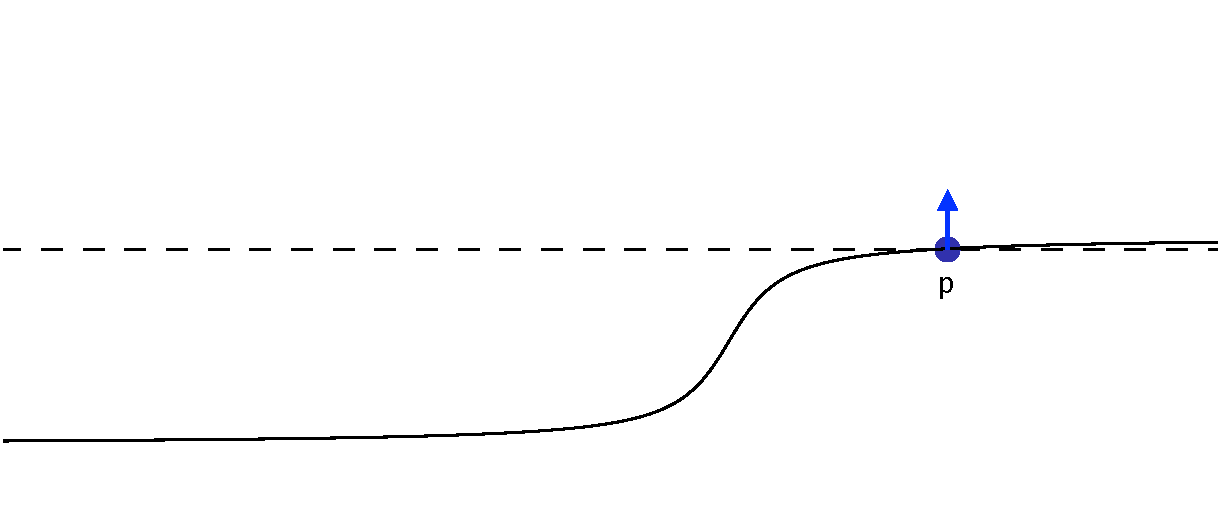
\includegraphics[width=\linewidth]{fig/curvature_distances.pdf}
	\caption{Large $\sum d_i$, small $\sum |\alpha_i|$}
\end{subfigure}%
\hspace{15mm}%
\begin{subfigure}{.4\textwidth}
	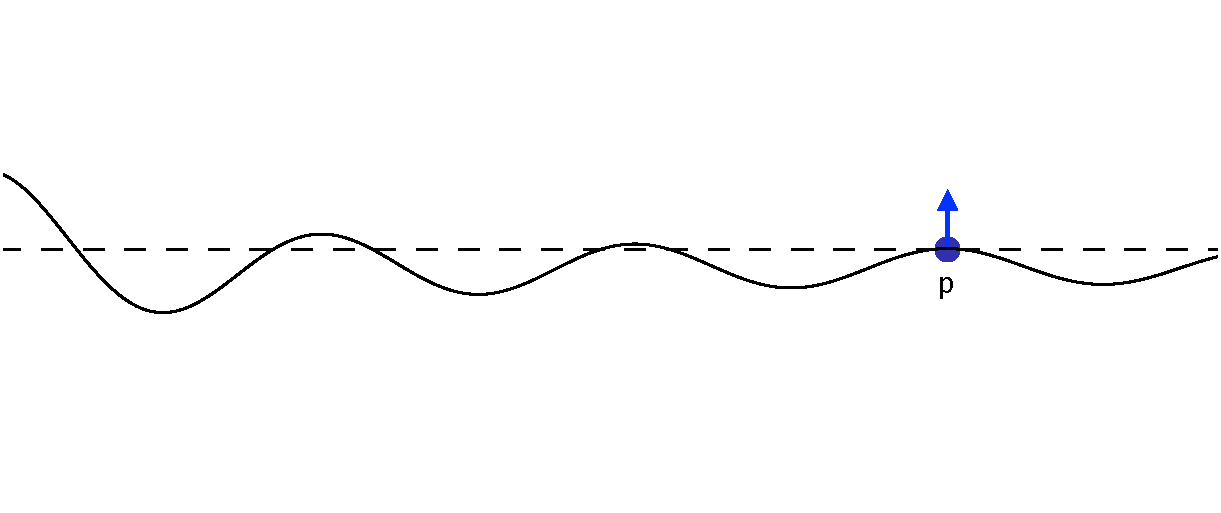
\includegraphics[width=\linewidth]{fig/curvature_angles.pdf}
	\caption{Large $\sum |\alpha_i|$, small $\sum d_i$}
\end{subfigure}	
\end{figure}
For the purposes that the curvature measure is used here, $A$ should be set higher, because surfaces such as the left-side can still be considered to be locally planar.






\subsection{Point dispersion}
Point dispersion refers to how points in a point clouds are arranged on a surface. When the surface is locally planar, regions of the surface can be approximated by a plane. The following three point dispersions on the plane will be analyzed:
\begin{figure}[H]
\centering
\hspace*{\fill}%
\begin{subfigure}{.3\textwidth}
{
	\setlength{\fboxsep}{0pt}%
	\setlength{\fboxrule}{0.5pt}%
	\fbox{
\includegraphics[width=\linewidth]{fig/dispersion_random.png}}%
	\caption{Random dispersion}
}
\end{subfigure}%
\hfill%
\begin{subfigure}{.3\textwidth}
{
	\setlength{\fboxsep}{0pt}%
	\setlength{\fboxrule}{0.5pt}%
	\fbox{
\includegraphics[width=\linewidth]{fig/dispersion_sqgrid.png}}%
	\caption{Square grid}
}
\end{subfigure}%
\hfill%
\begin{subfigure}{.3\textwidth}
{
	\setlength{\fboxsep}{0pt}%
	\setlength{\fboxrule}{0.5pt}%
	\fbox{
\includegraphics[width=\linewidth]{fig/dispersion_pargrid.png}}%
	\caption{Parallelogram grid}
}%
\end{subfigure}\\
\caption{Different point dispersions on planar surface}
\label{fig:point_dispersion}
\end{figure}

The \emph{random dispersion} is the most general case, where the $x$ and $y$ coordinates of each points are independent, random variables, with a uniform distribution. It can be seen visually that the local density in that case is not constant.

Point clouds recorded by a laser scanner will produce a dispersion that is more akin to the \emph{square grid dispersion}. If the scanner processes in sequential scan-lines, and uses a regular graduation of azimuth and elevation coordinates, a planar surface placed perpendicular to the scanner ray will \emph{locally} get points approximatively arranged in squares. The dispersion will be considered to be invariant to a two-dimensional rotation of the plane itself.

\subsection{Parallelogram grid}
When the surface is placed at an oblique angle to the scanner line, the points on the plane will instead be dispersed on a \emph{parallelogram grid}. Figures \ref{fig:closeup_ddp}, \ref{fig:closeup_wall} show two close-up views of the ``Hôtel de Ville'' scans, featuring the parallelogram grid point dispersion on approximatively planar surfaces. Figure \ref{fig:bunny_grid_closeup} is taken from the Stanford Bunny point cloud, which was also recorded using a laser scanner. The square grid or rectangular grid are special case of this.

\begin{figure}[p]
\centering
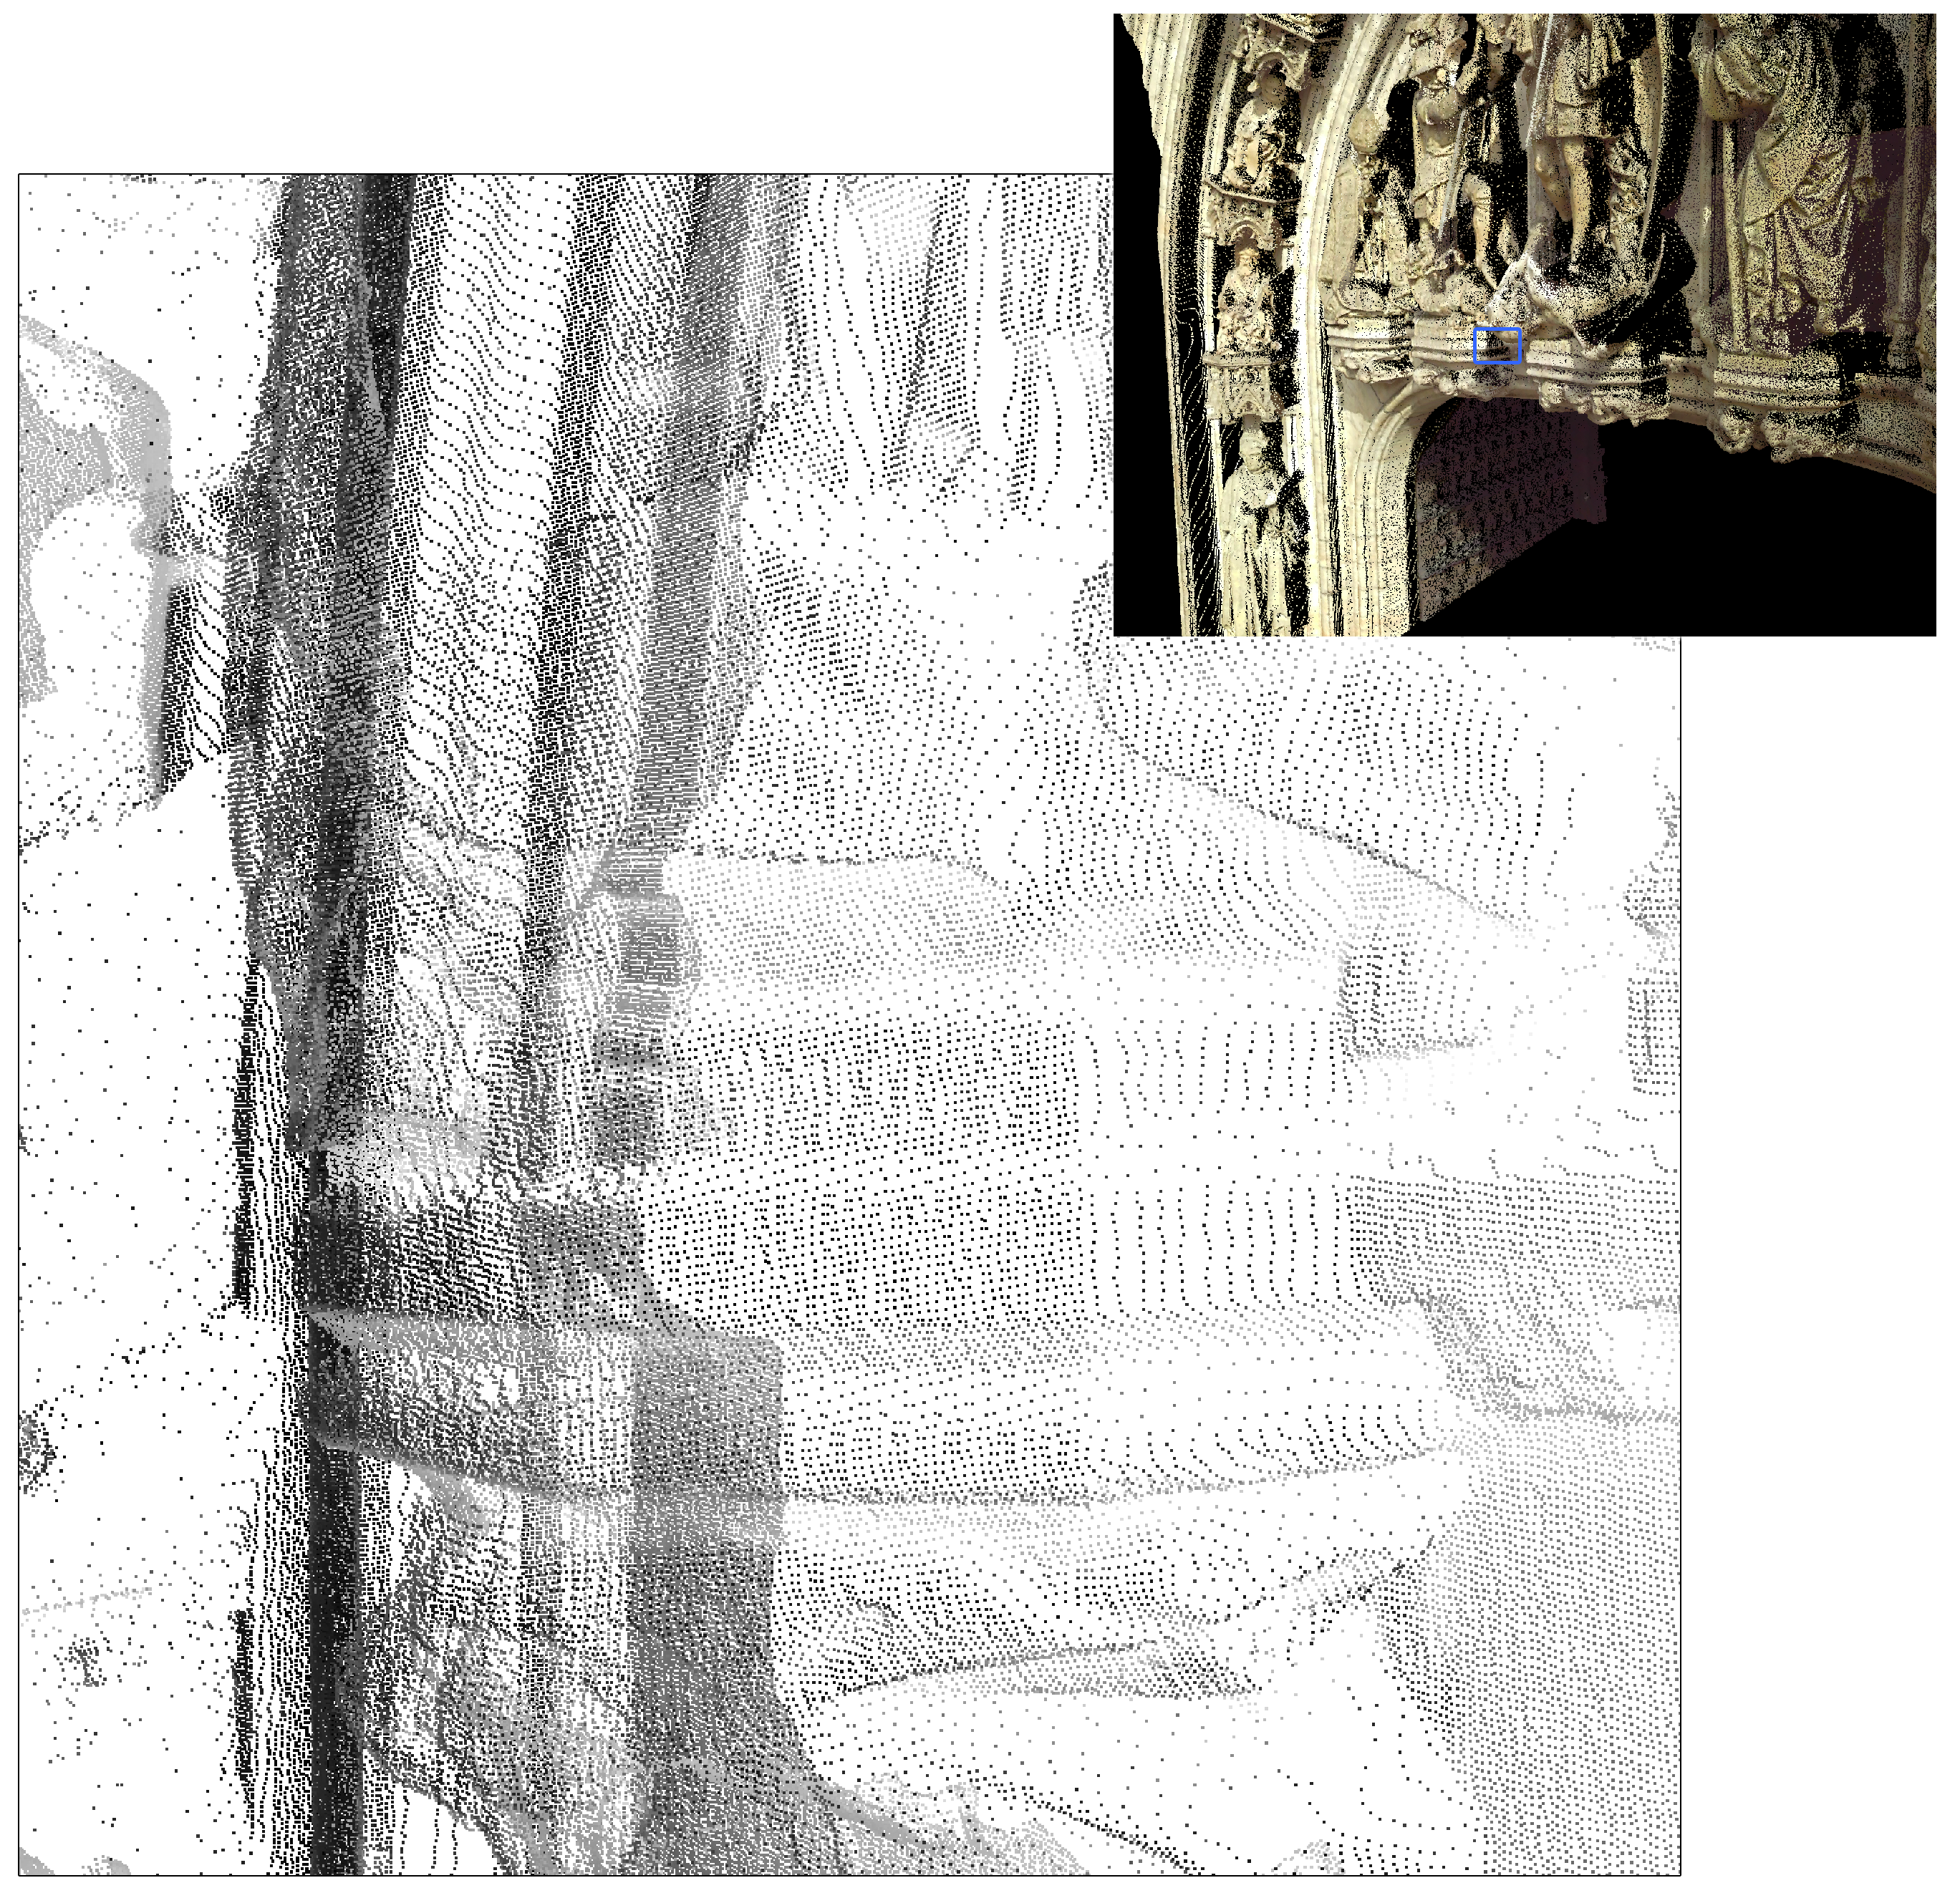
\includegraphics[width=.6\textwidth]{fig/closeup_ddp.png}
\caption{Closeup of the surface distribution of points on front wall of building}
\label{fig:closeup_ddp}
\end{figure}

\begin{figure}[p]
\centering
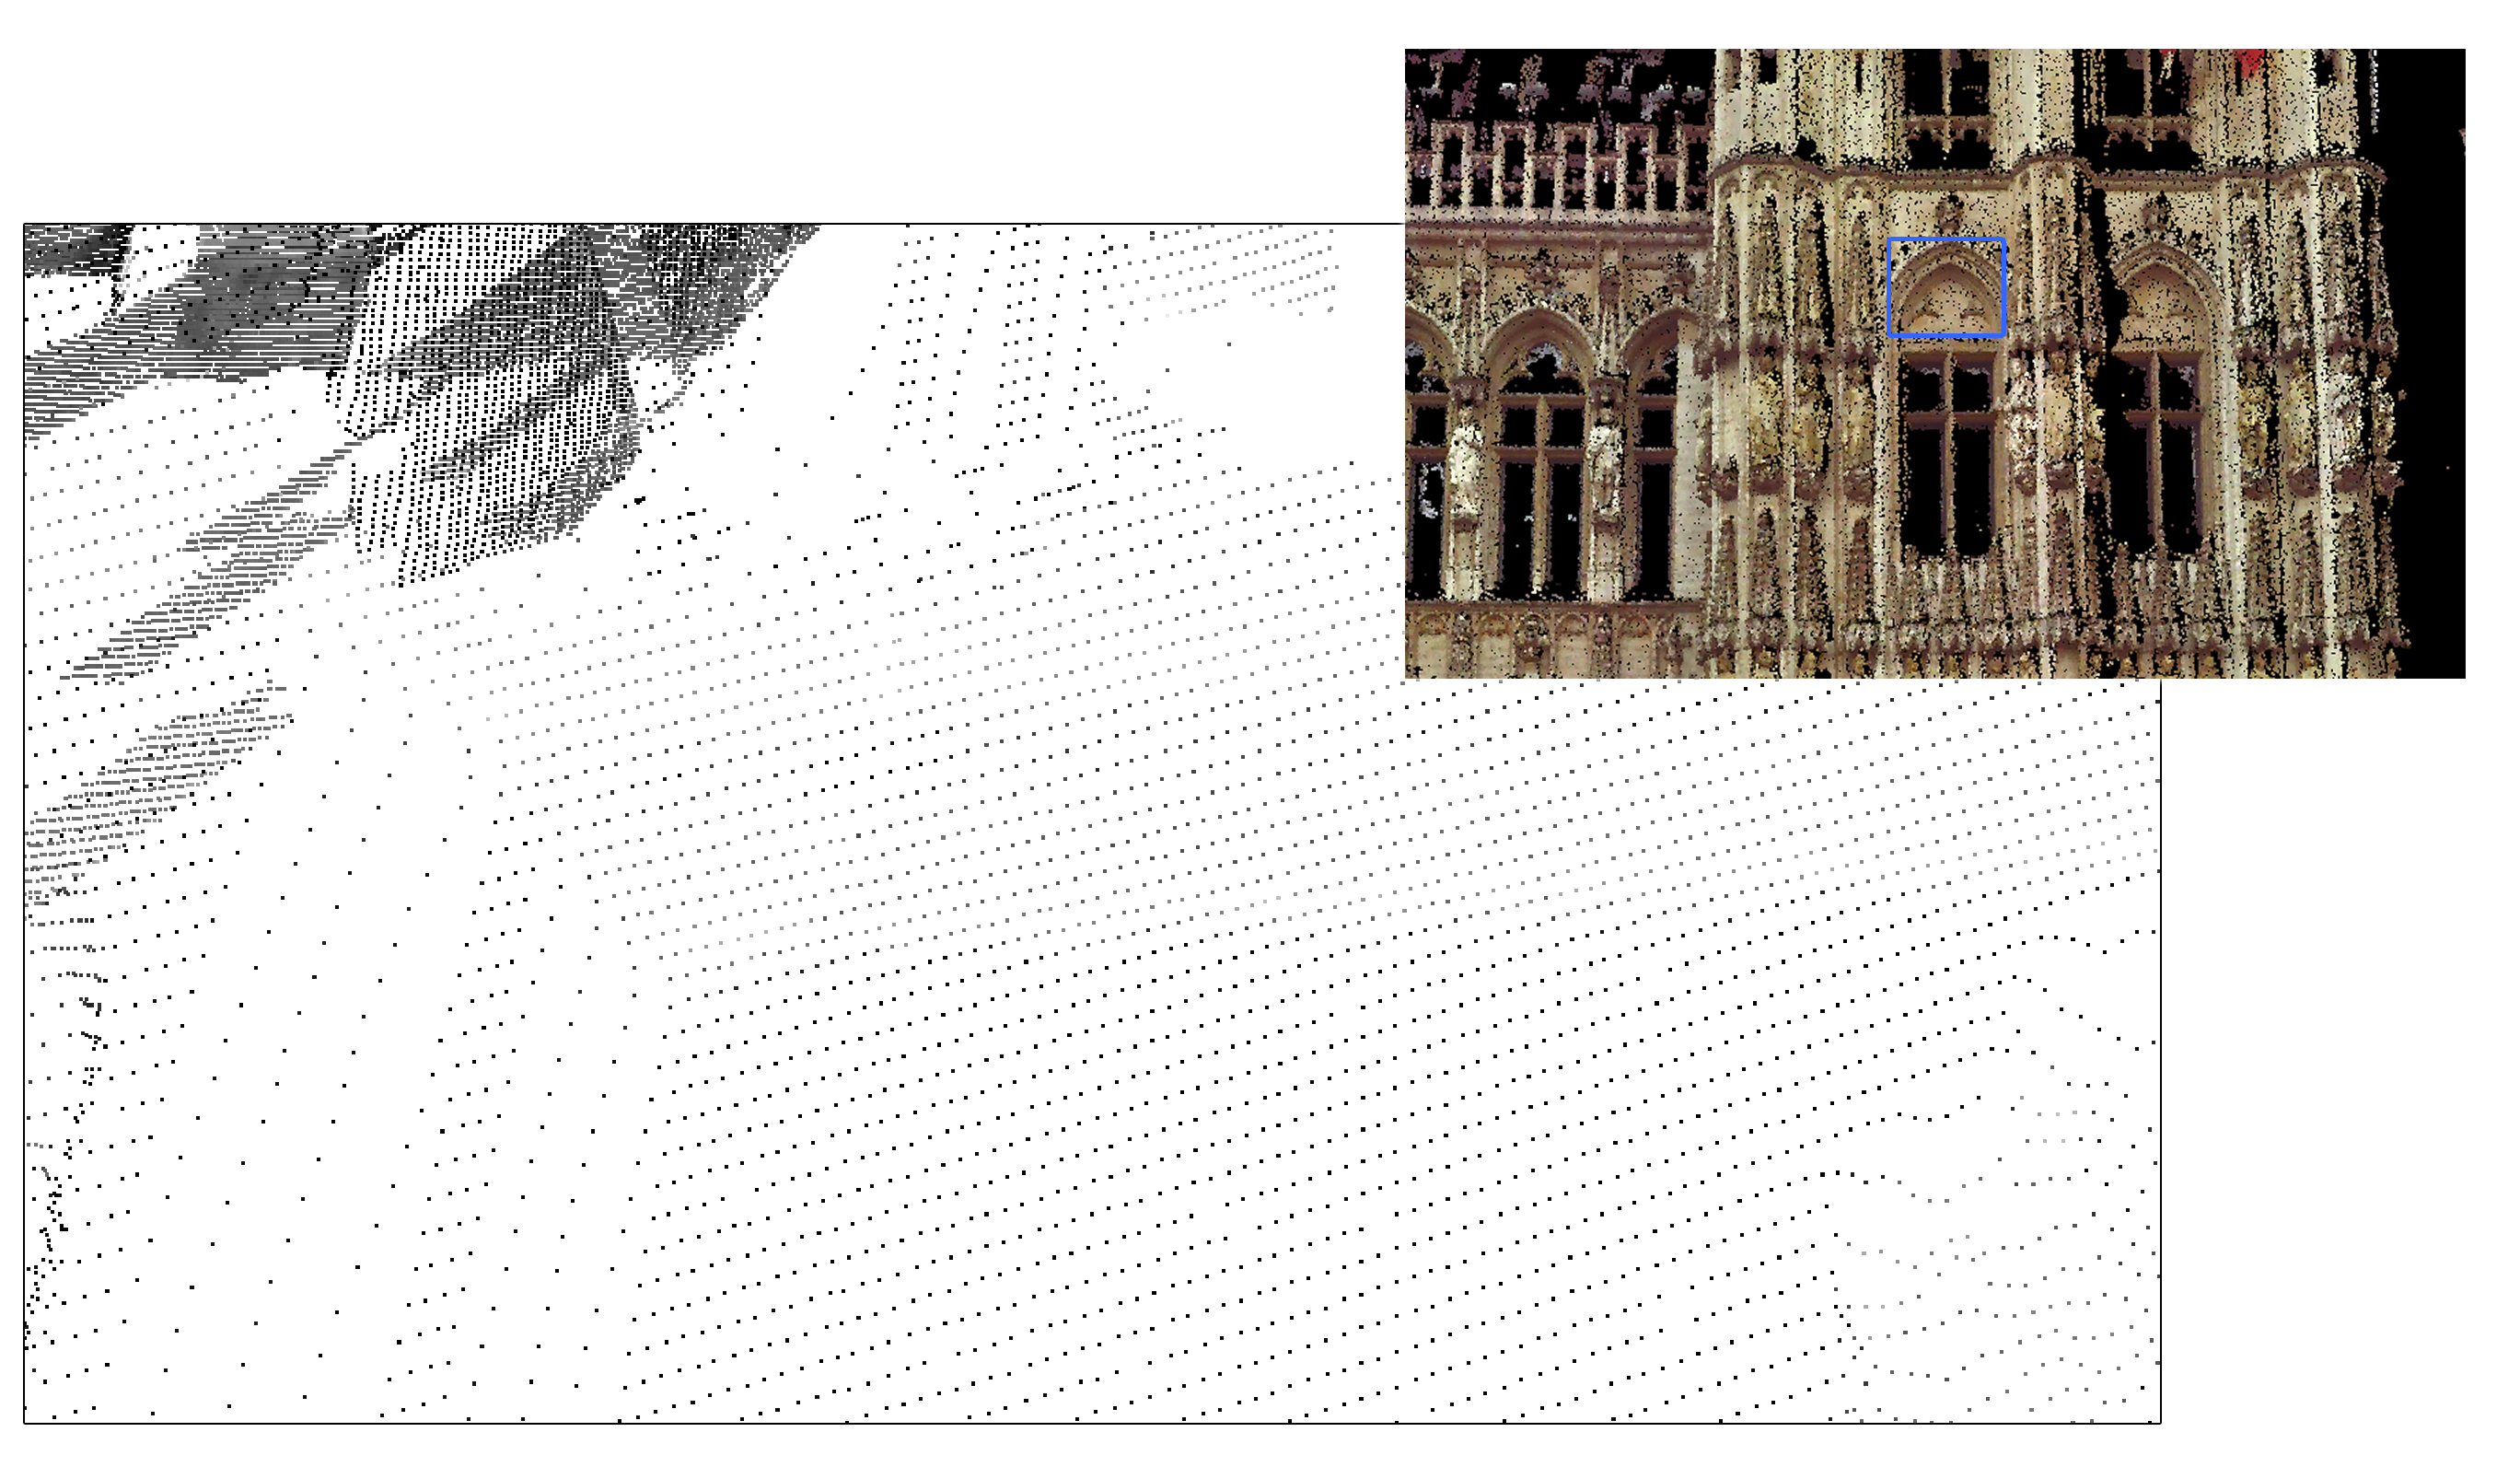
\includegraphics[width=.6\textwidth]{fig/closeup_wall.png}
\caption{Closeup of the surface distribution of points on detail of ``dessus-de-porte''}
\label{fig:closeup_wall}
\end{figure}

\begin{figure}[p]
\centering
{
	\setlength{\fboxsep}{0pt}%
	\setlength{\fboxrule}{0.5pt}%
	\fbox{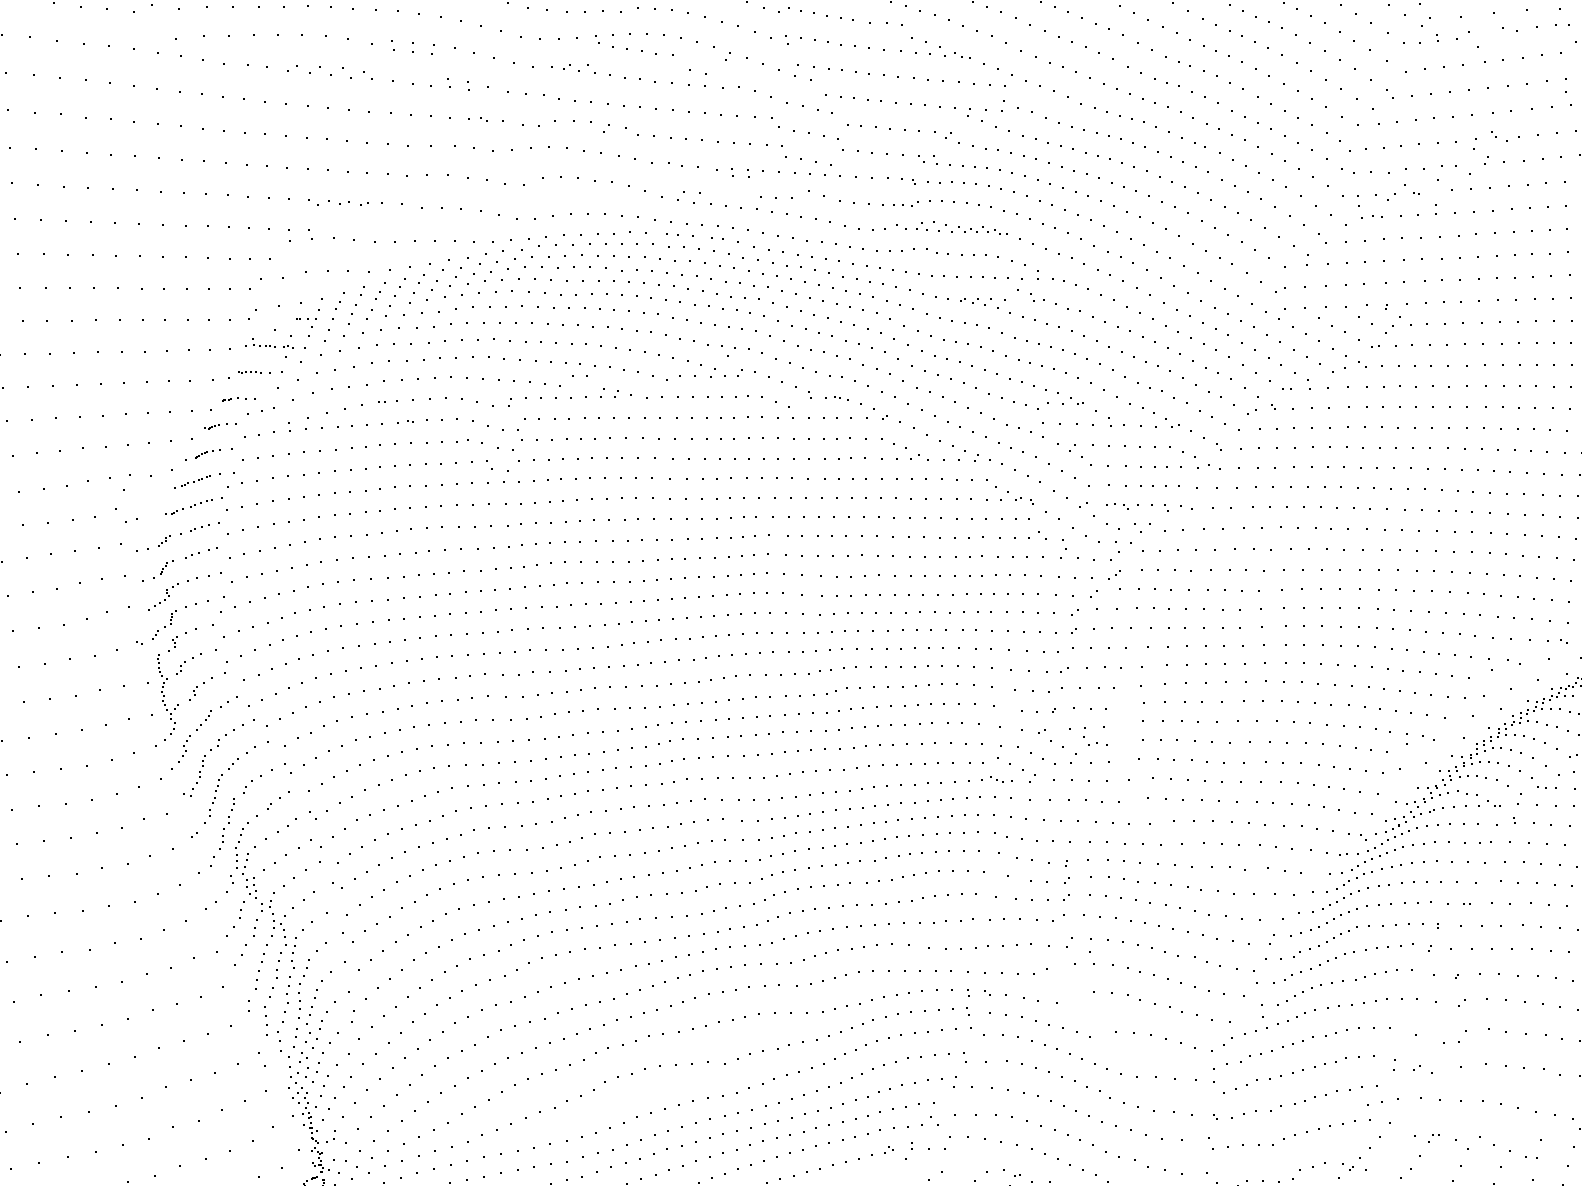
\includegraphics[width=.4\textwidth]{fig/bunny_grid_closeup.png}}
}
\caption{Closeup of the surface distribution of points on Bunny point cloud}
\label{fig:bunny_grid_closeup}
\end{figure}

The diagram on figure \ref{fig:pargrid_proj} shows the parallel projection of a square from camera image space onto a plane in three-dimensional space. $\vec{n}$ is the normal vector of the plane, $p_l$ the width and height (side length) of the square, and $x, y$ the corresponding side lengths of the projected square. It can be seen that the projected square takes on the shape of a parallelogram on the plane. This models the projection of scanner rays on a surface. The coordinate system is such that the scanner is placed at origin. Since only a small region of a locally planar surface is considered (compared to the field of view of the scanner), adjacent rays in azimuth and elevation direction are modeled as parallel. When the square is extended to form a square grid in the XY-plane, a parallelogram grid is formed on the plane in which all parallelograms have the same two side lengths and inner angles.

\begin{figure}[h]
\centering
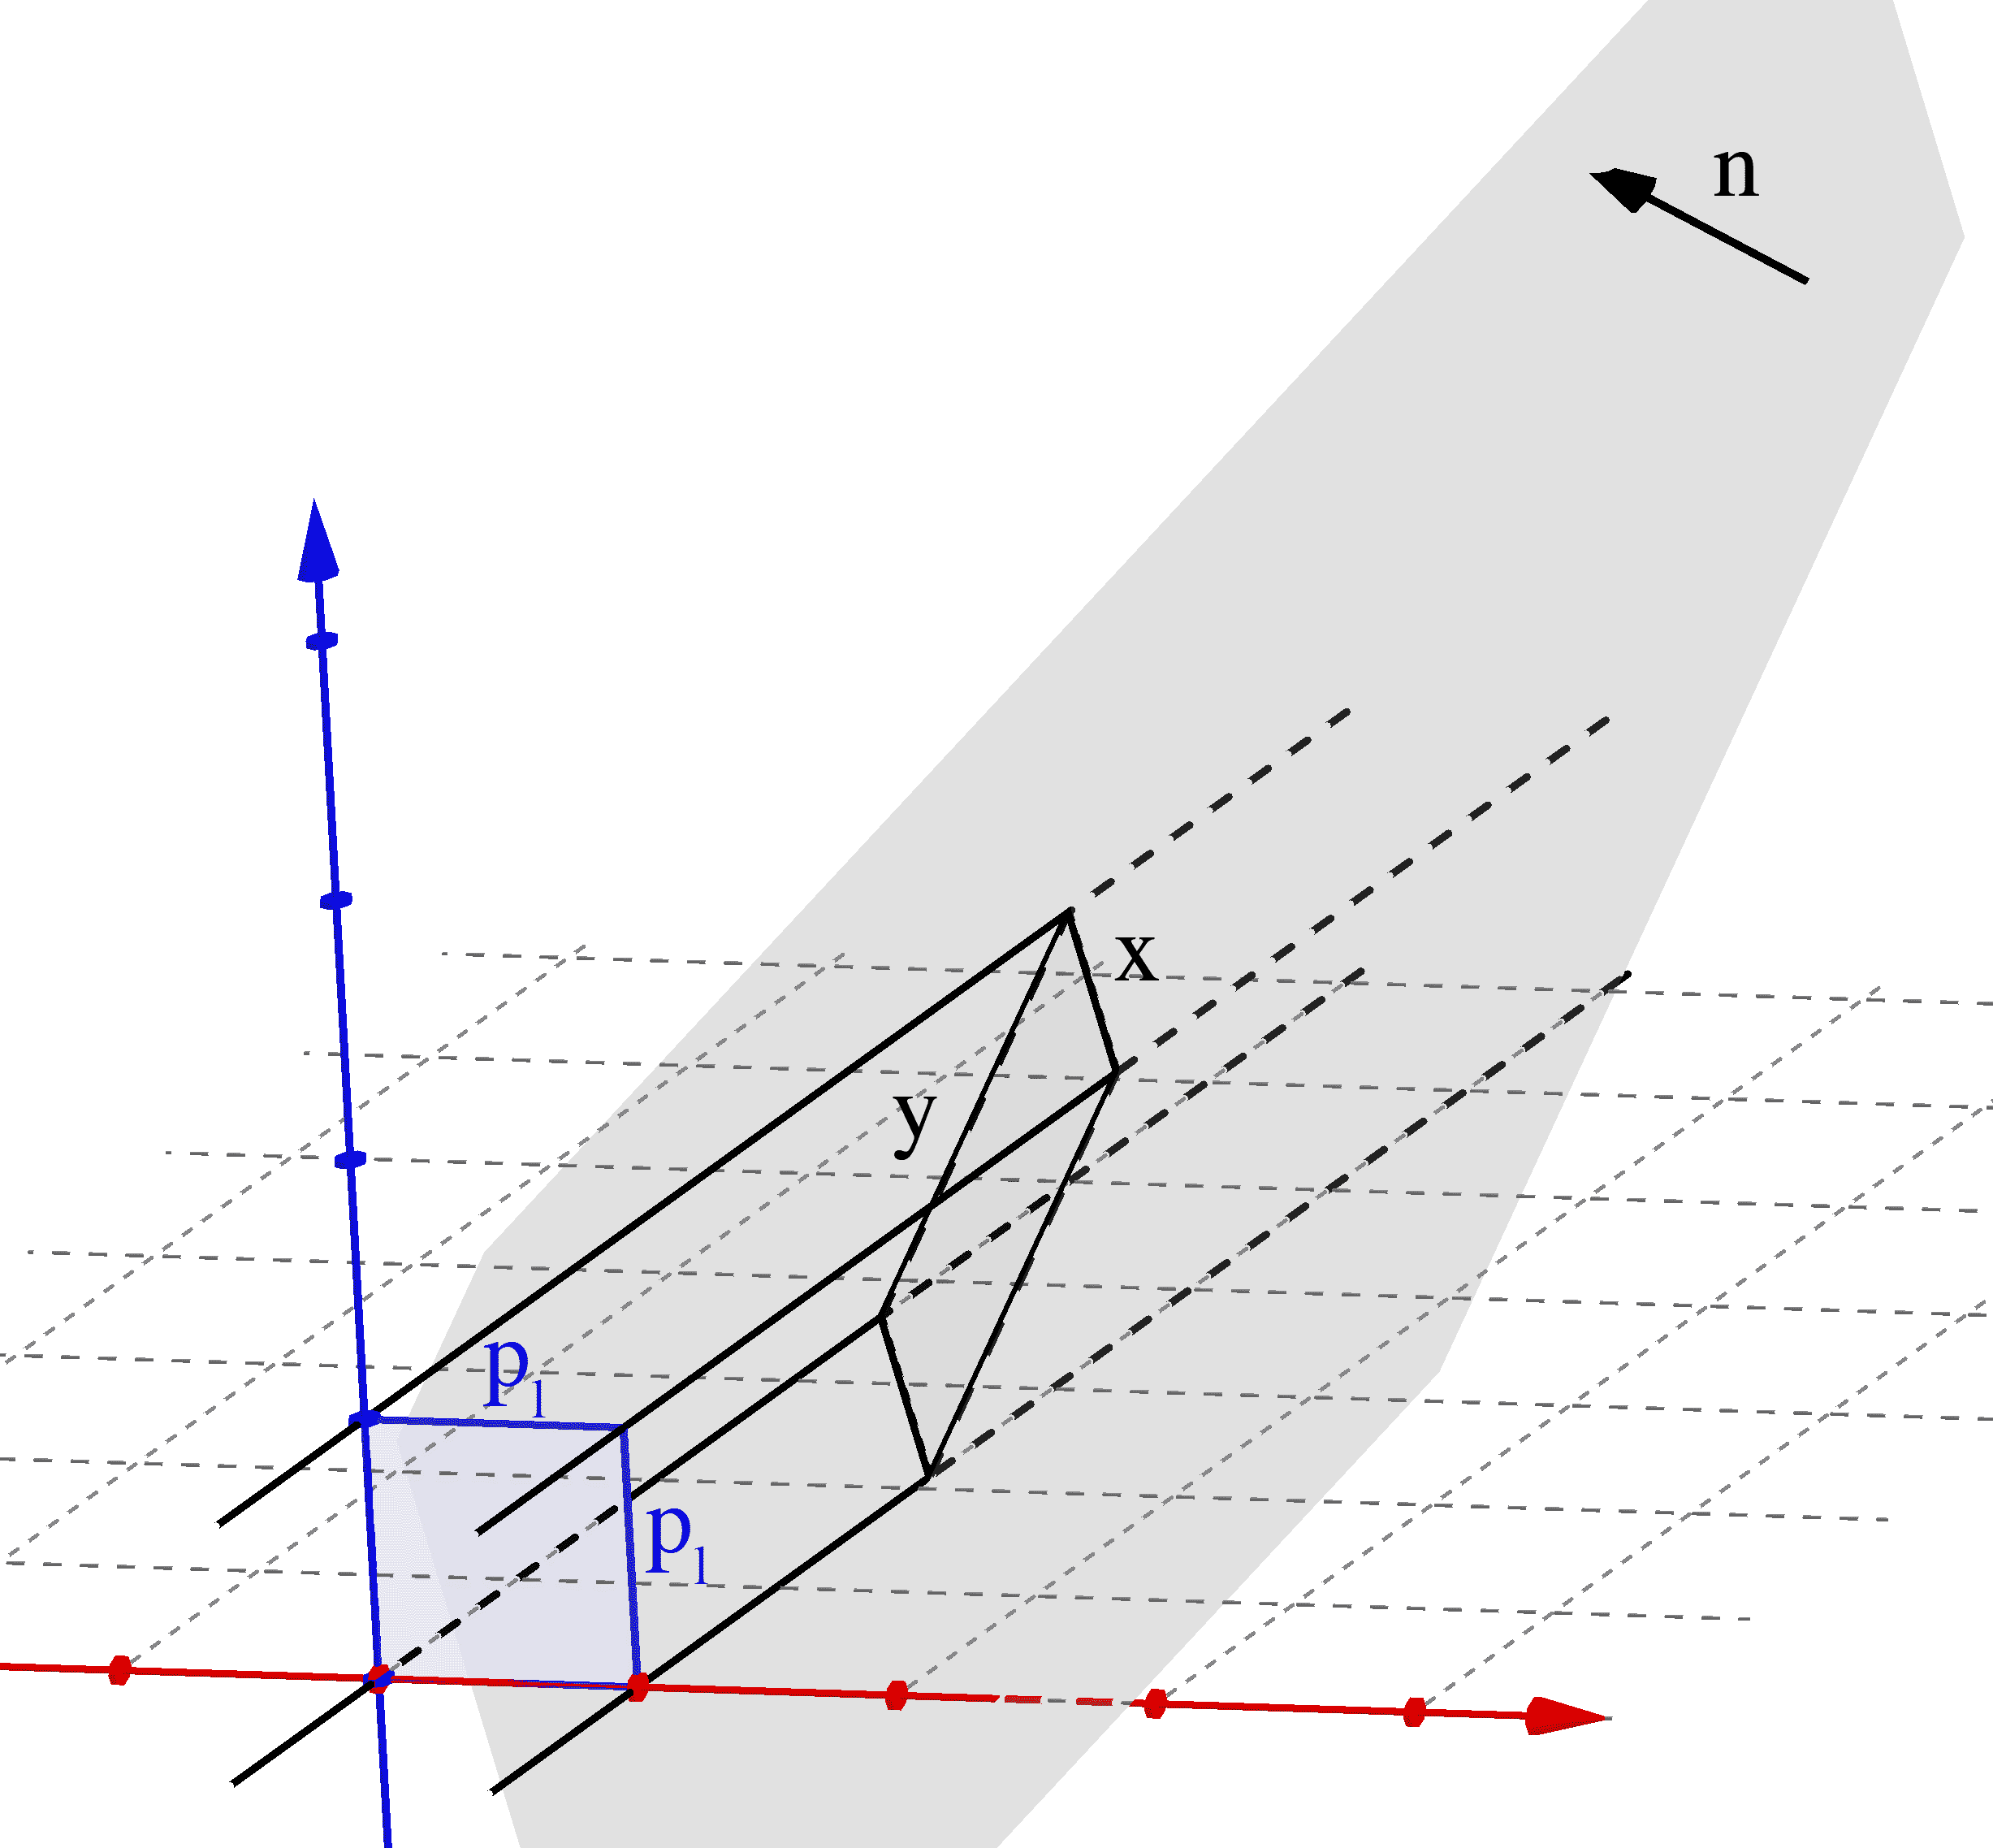
\includegraphics[width=.4\textwidth]{fig/pargrid_proj.png}
\caption{Parallel projection of square onto plane in space}
\label{fig:pargrid_proj}
\end{figure}

It can be seen on figure \ref{fig:par_grid_tilings} that several different parallelogram grids are possible for the same dispersion of points on the plane. The two grids in these examples have no sides in common. The projection of the camera square grid on the plane results in one of the possible parallel grids. When the plane is placed at a more oblique angle from the camera, it tends to be a grid with longer side lengths, such as the second on on the figure. It is not necessarily such that it includes the shortest possible parallelogram edge.

\begin{figure}[h]
\centering
\hspace*{\fill}%
\begin{subfigure}{.33\textwidth}
{
	\setlength{\fboxsep}{0pt}%
	\setlength{\fboxrule}{0.5pt}%
	\fbox{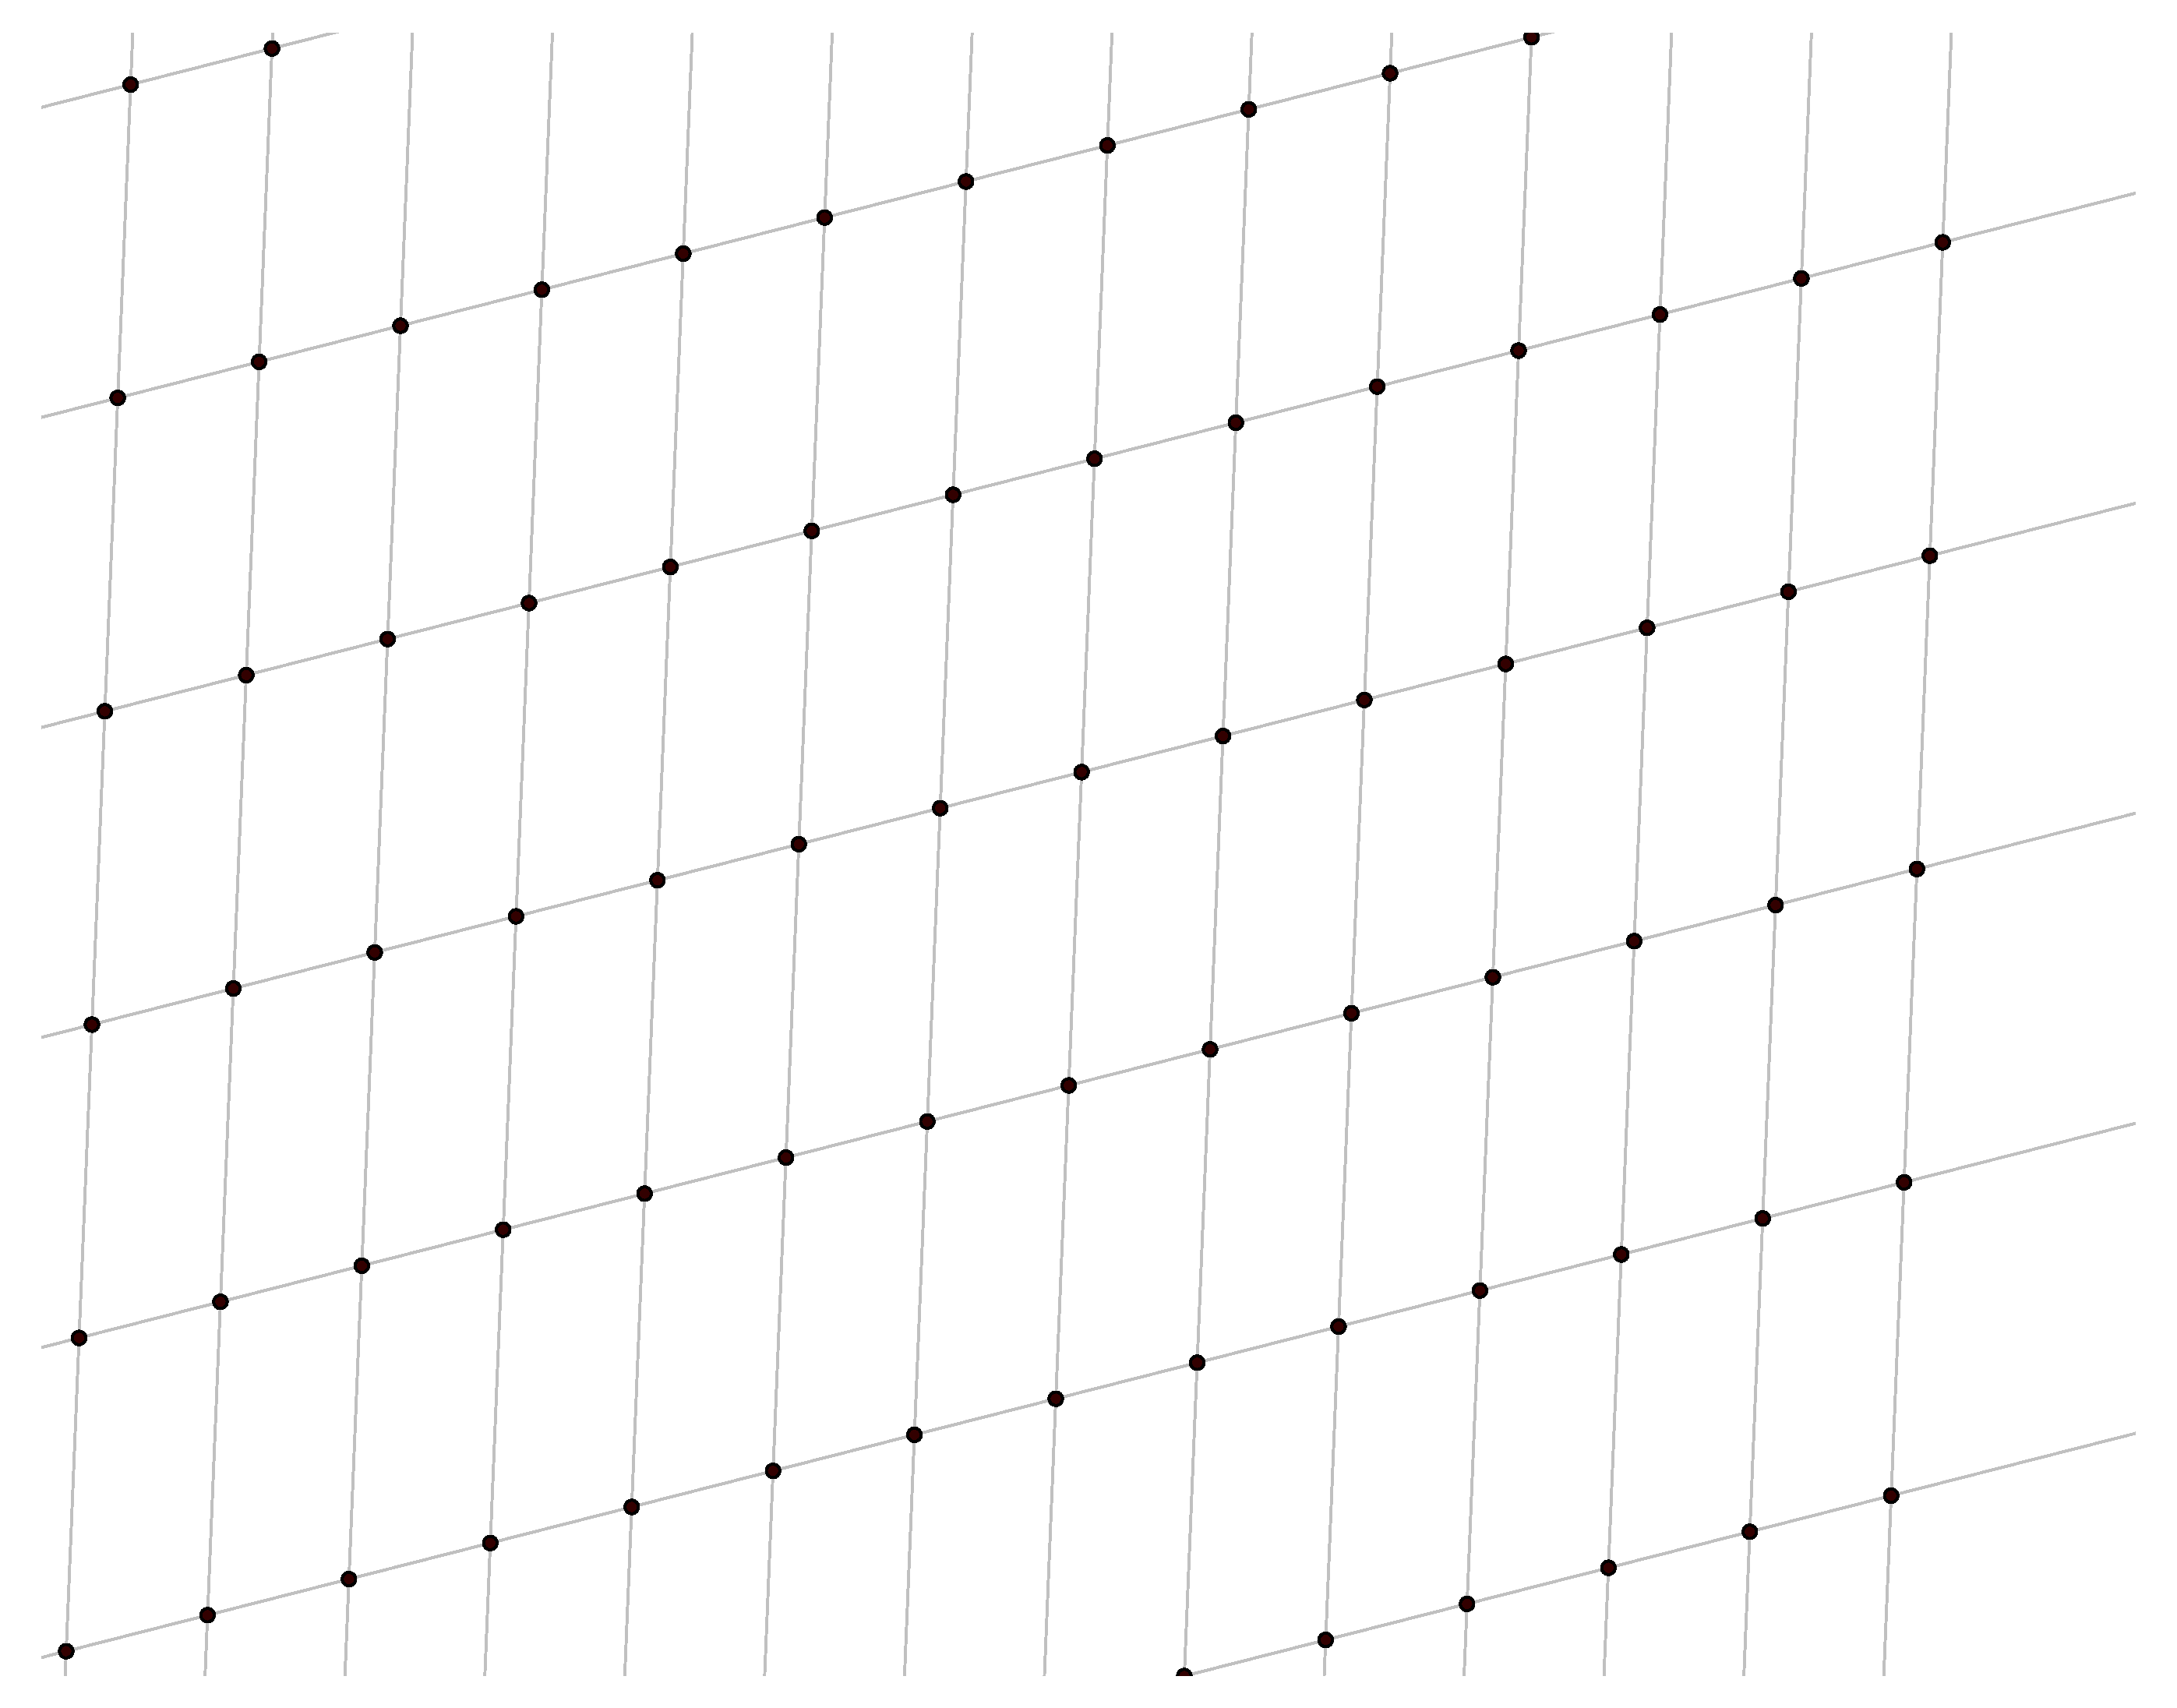
\includegraphics[trim=30 20 180 20, clip, width=\linewidth]{fig/pargrid1.pdf}}
}\end{subfigure}%
\hfill%
\begin{subfigure}{.33\textwidth}
{
	\setlength{\fboxsep}{0pt}%
	\setlength{\fboxrule}{0.5pt}%
	\fbox{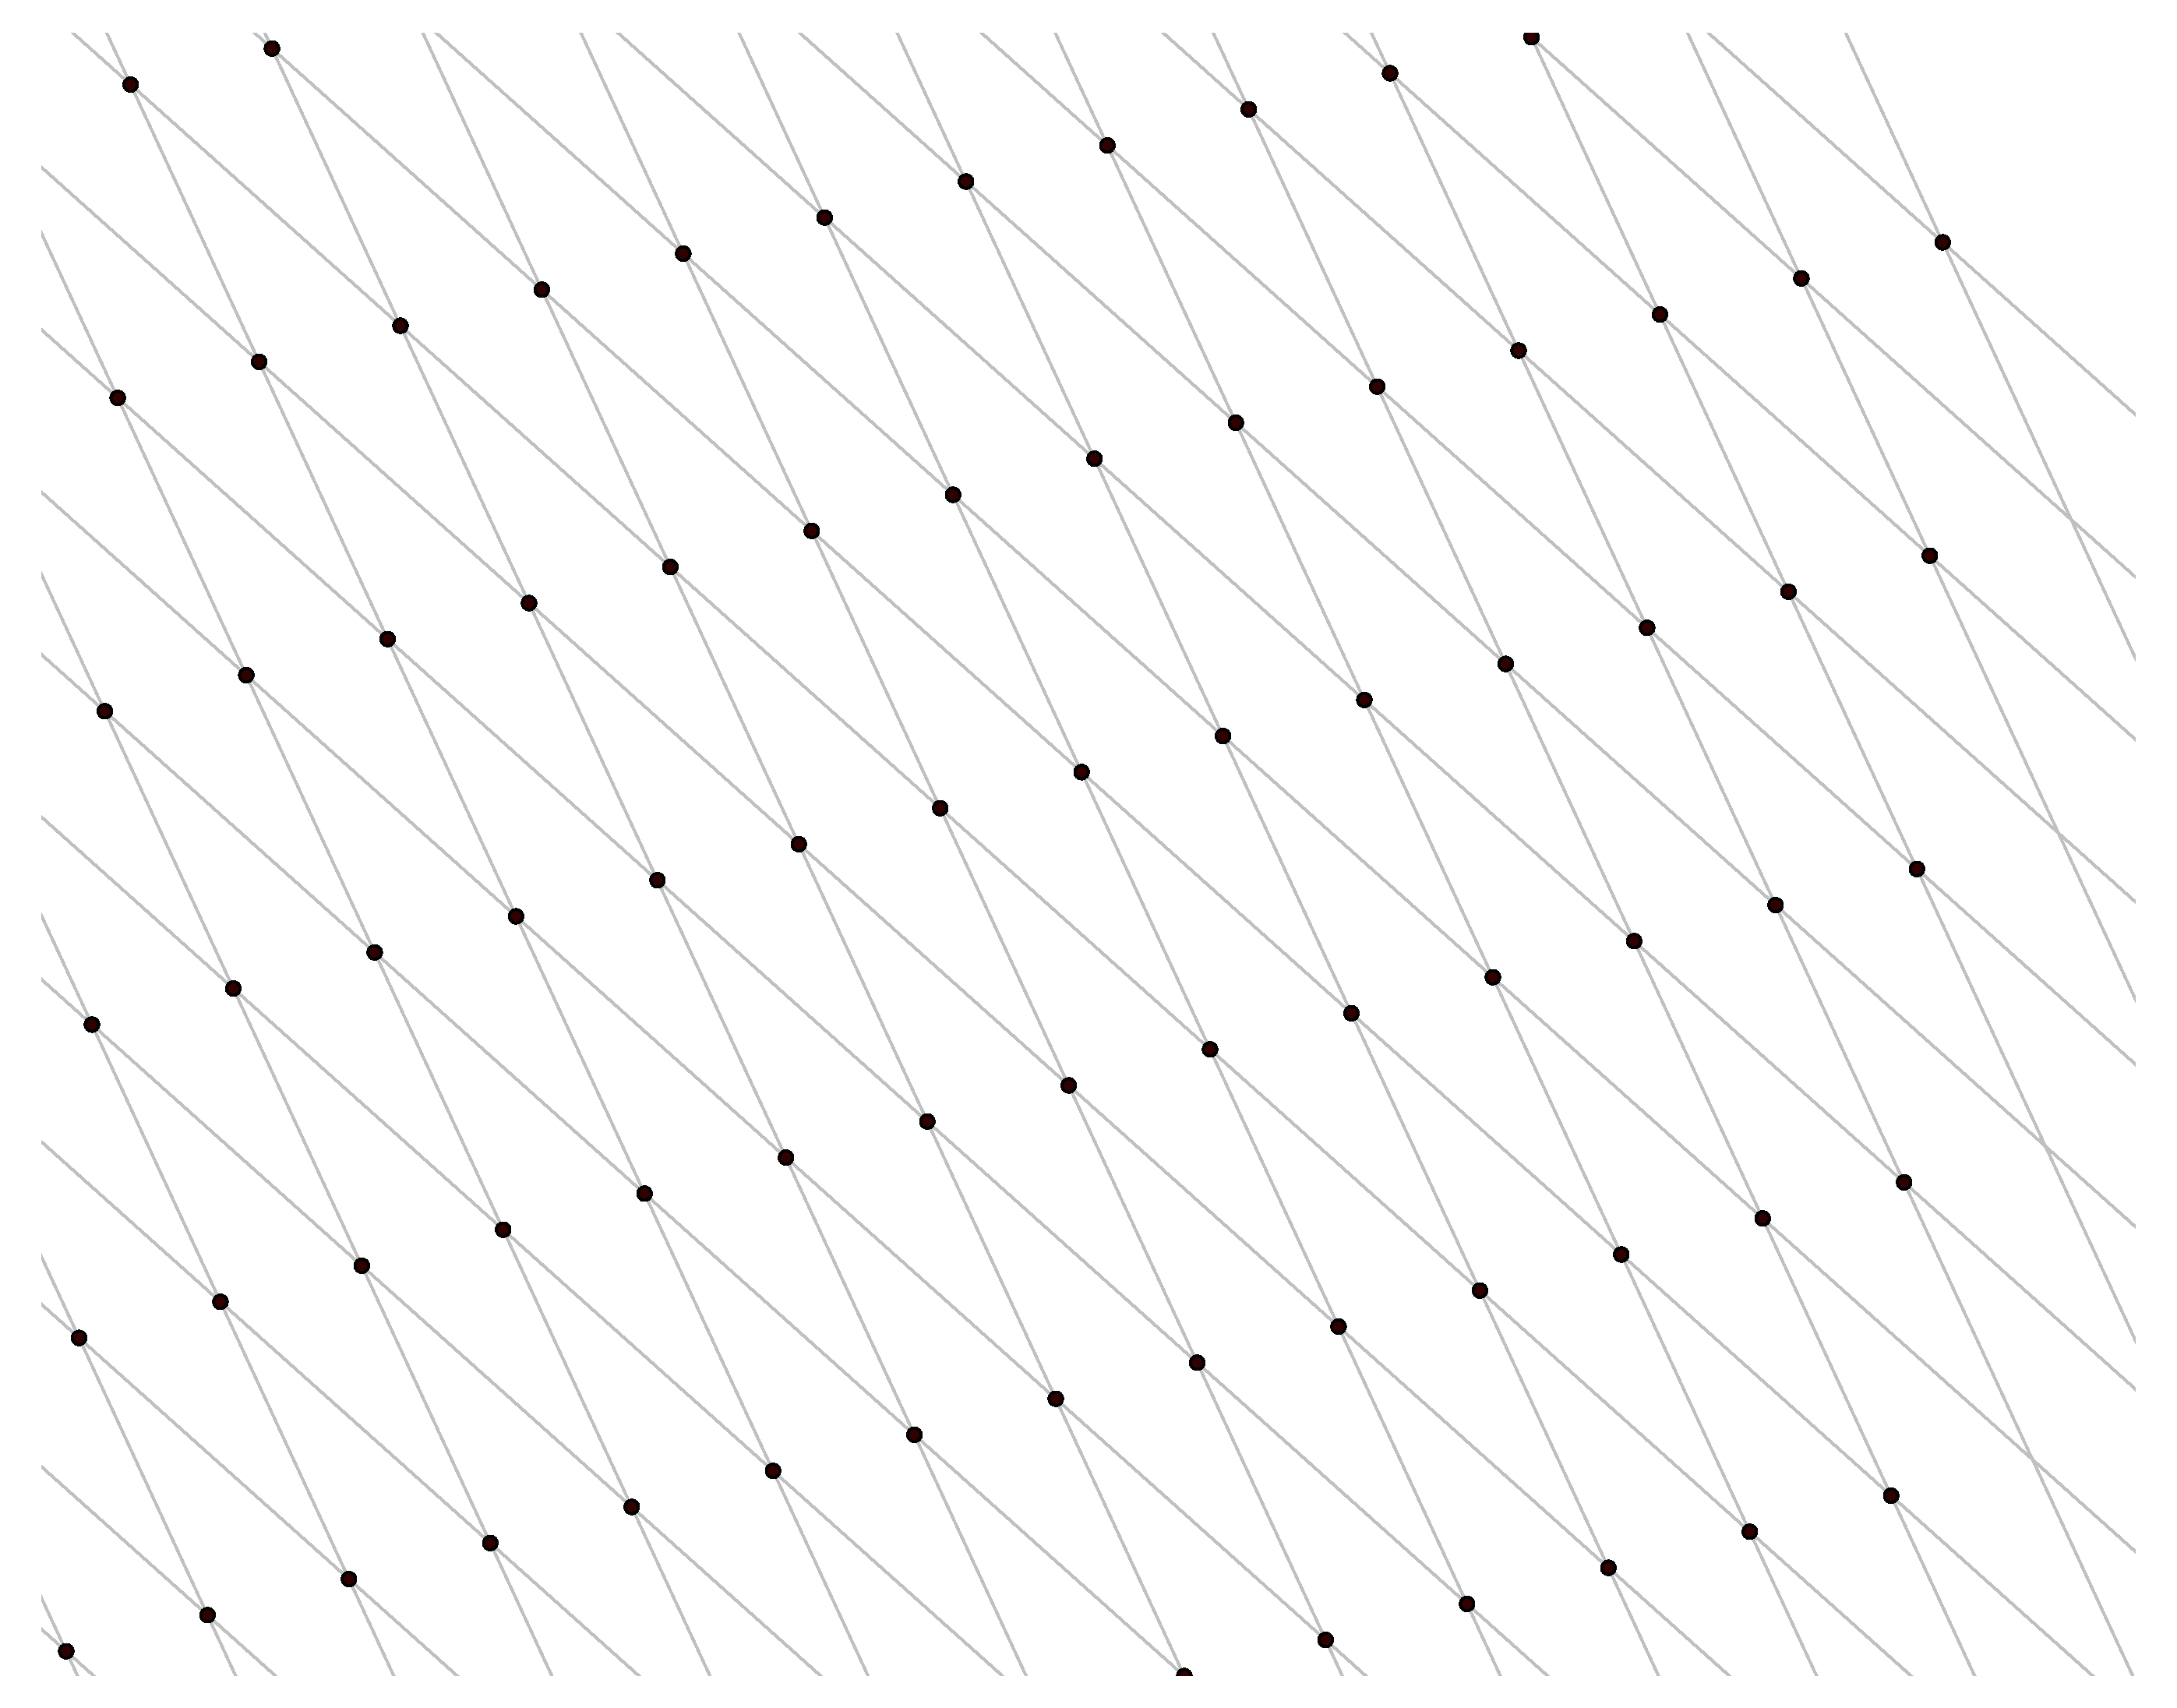
\includegraphics[trim=30 20 180 20, clip, width=\linewidth]{fig/pargrid2.pdf}}
}\end{subfigure}%
\hspace*{\fill}
\caption{Different parallelogram grids for same point dispersion}
\label{fig:par_grid_tilings}
\end{figure}


\subsubsection{Measures}
Three measures on the point dispersion will be used: (1) The point density $\rho$. (2) The shortest possible parallelogram side length $l_{\text{min}}$, for any parallelogram grid put on the points. It corresponds to the distance from any point to its closest neighbor. (3) The maximal distance $d_{\text{max}}$ from any position on the plane to the closest point of the dispersion.

These values can be calculated from the normal vector $\vec{n}$, and the square grid side length on image space $p_l$ as follows. Proofs for these formulea are given in appendix \ref{sec:proof_pargrid_measures}.
\begin{equation}
\rho = \frac{| n_z |}{p^2_l}
\end{equation}
\begin{equation} \label{eq:pargrid_lmin}
l_{\text{min}} = p_l \times \min \left\{
\sqrt{1 + \left( \frac{n_x}{n_z} \right)^2},
\sqrt{1 + \left( \frac{n_y}{n_z} \right)^2},
\sqrt{2 + \left( \frac{n_x + n_y}{n_z} \right)^2},
\sqrt{2 + \left( \frac{n_x - n_y}{n_z} \right)^2}
\right\}
\end{equation} 
\begin{equation}
d_{\text{max}} = p_l \times \min \frac{\sqrt{ (1 \pm 2 \, n_x \, n_y + n^2_z) \, (1 - n^2_y) \, (n^2_y + n^2_z) }}{4 \, n^2_z}
\end{equation} 

\subsubsection{Analysis}
Figure \ref{fig:lmin_plot} shows the value $l_{\text{min}}$, in function of the normal vector $\vec{n}$ of the plane. For the grayscale tones a logarithmic scale is used. Darker tones correspond to lower values. The $x$ and $y$ axis of the plot correspond to $n_x$ and $n_y$, the third component is set to $n_z = \sqrt{1 - n^2_x - n^2_y}$. The plot is symmetric around the X and Y axis. The origin point $(0, 0)$ corresponds to $\vec{n} = \transpose{(0, 0, 1)}$, that is, the plane is perpendicular to the camera ray and has a square grid dispersion. Then $l_{\text{min}} = 1$, the side length of the square. For the points on either axis, the plane is turned on one direction only, resulting in a rectangular grid, where the shortest side remains $l_{\text{min}} = 1$. Around the border of the plot, the plane is nearly parallel to the camera rays. When $n_x \approx n_y$, the parallelograms take on a rhombus shape, similar to the second grid shown on figure \ref{fig:par_grid_tilings}. The shortest edge becomes the projection of the squares' diagonal with length $\sqrt{2}$, whereas the projection of its sides results in longer edges.

\begin{figure}[p]
\centering
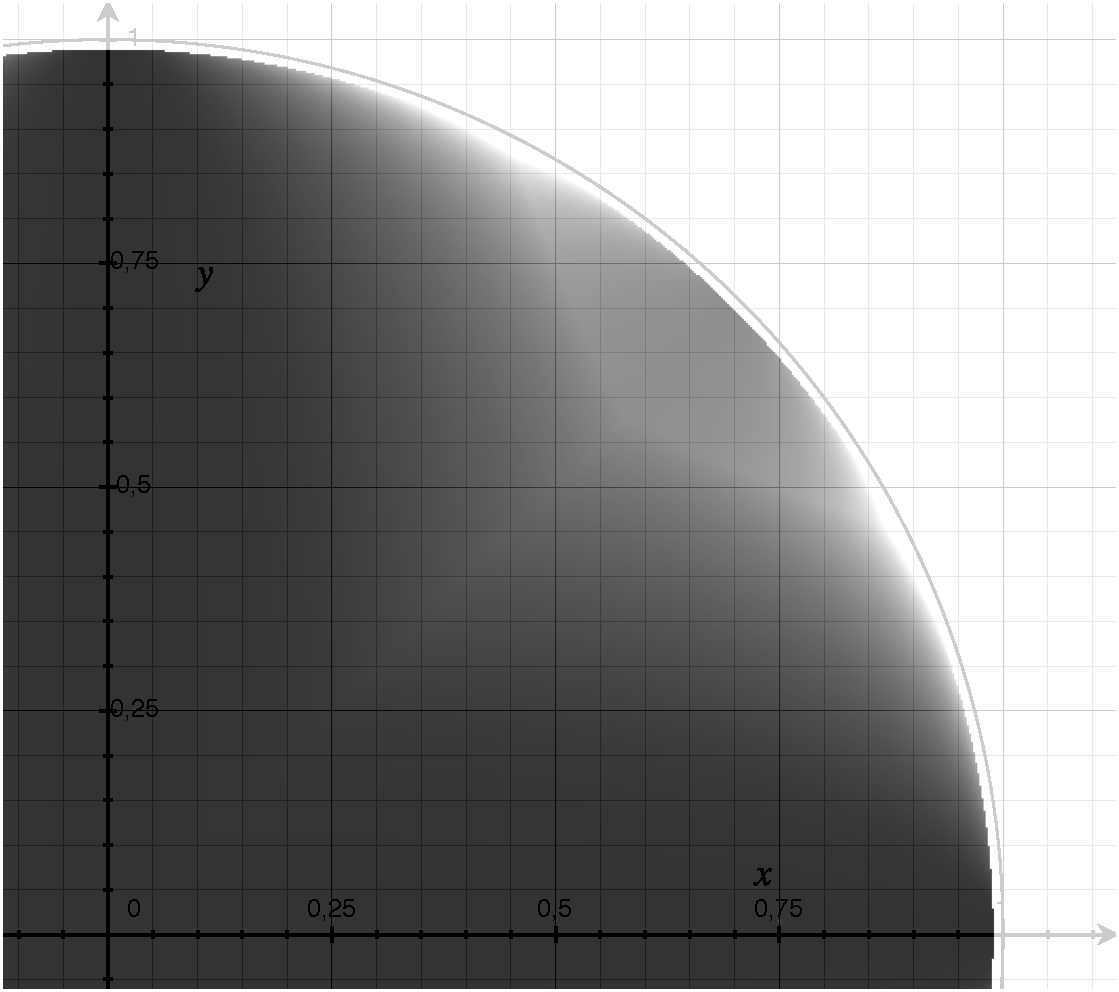
\includegraphics[width=.4\textwidth]{fig/lmin_plot.pdf}
\caption{Plot of $l_{\text{min}}$ for $\vec{n} = \transpose{(x, y, \sqrt{1 - x^2 - y^2})}$ and $p_l = 1$}
\label{fig:lmin_plot}
\end{figure}


\subsubsection{Verification}
The first (left-side) histogram on figure \ref{fig:relief_nn_hist} was generated by recording for each point $p \in P$ on a point cloud, the distance $d$ to its closest neighbor. (That is, the point $p' \in P$ such that $p' \neq p$ and $\| p - p' \|$ is minimal.) The point cloud $P$ used is a ``relief'' model as described before in section \ref{sec:art_relief}, projected without occlusion using a parallel projection camera with $p_l = 0.01$.

Two clusters for around $0.01$ for parts of the surface that are near-parallel to the camera rays, and around $0.0115$, where the surface is more oblique in both directions. Since the surface is not everywhere locally planar the histogram does not form sharp spikes.

For the second histogram the values $l_{\text{min}}$ are instead recorded using the normal vectors of the points $p \in P$, and with fixed $p_l = 0.01$. This histogram is generated solely by evaluating the formula \ref{eq:pargrid_lmin}, without looking at the coordinates of the points, or doing a closest neighbor search in $P$.

\begin{figure}[H]
\centering
\begin{subfigure}{.5\textwidth}
	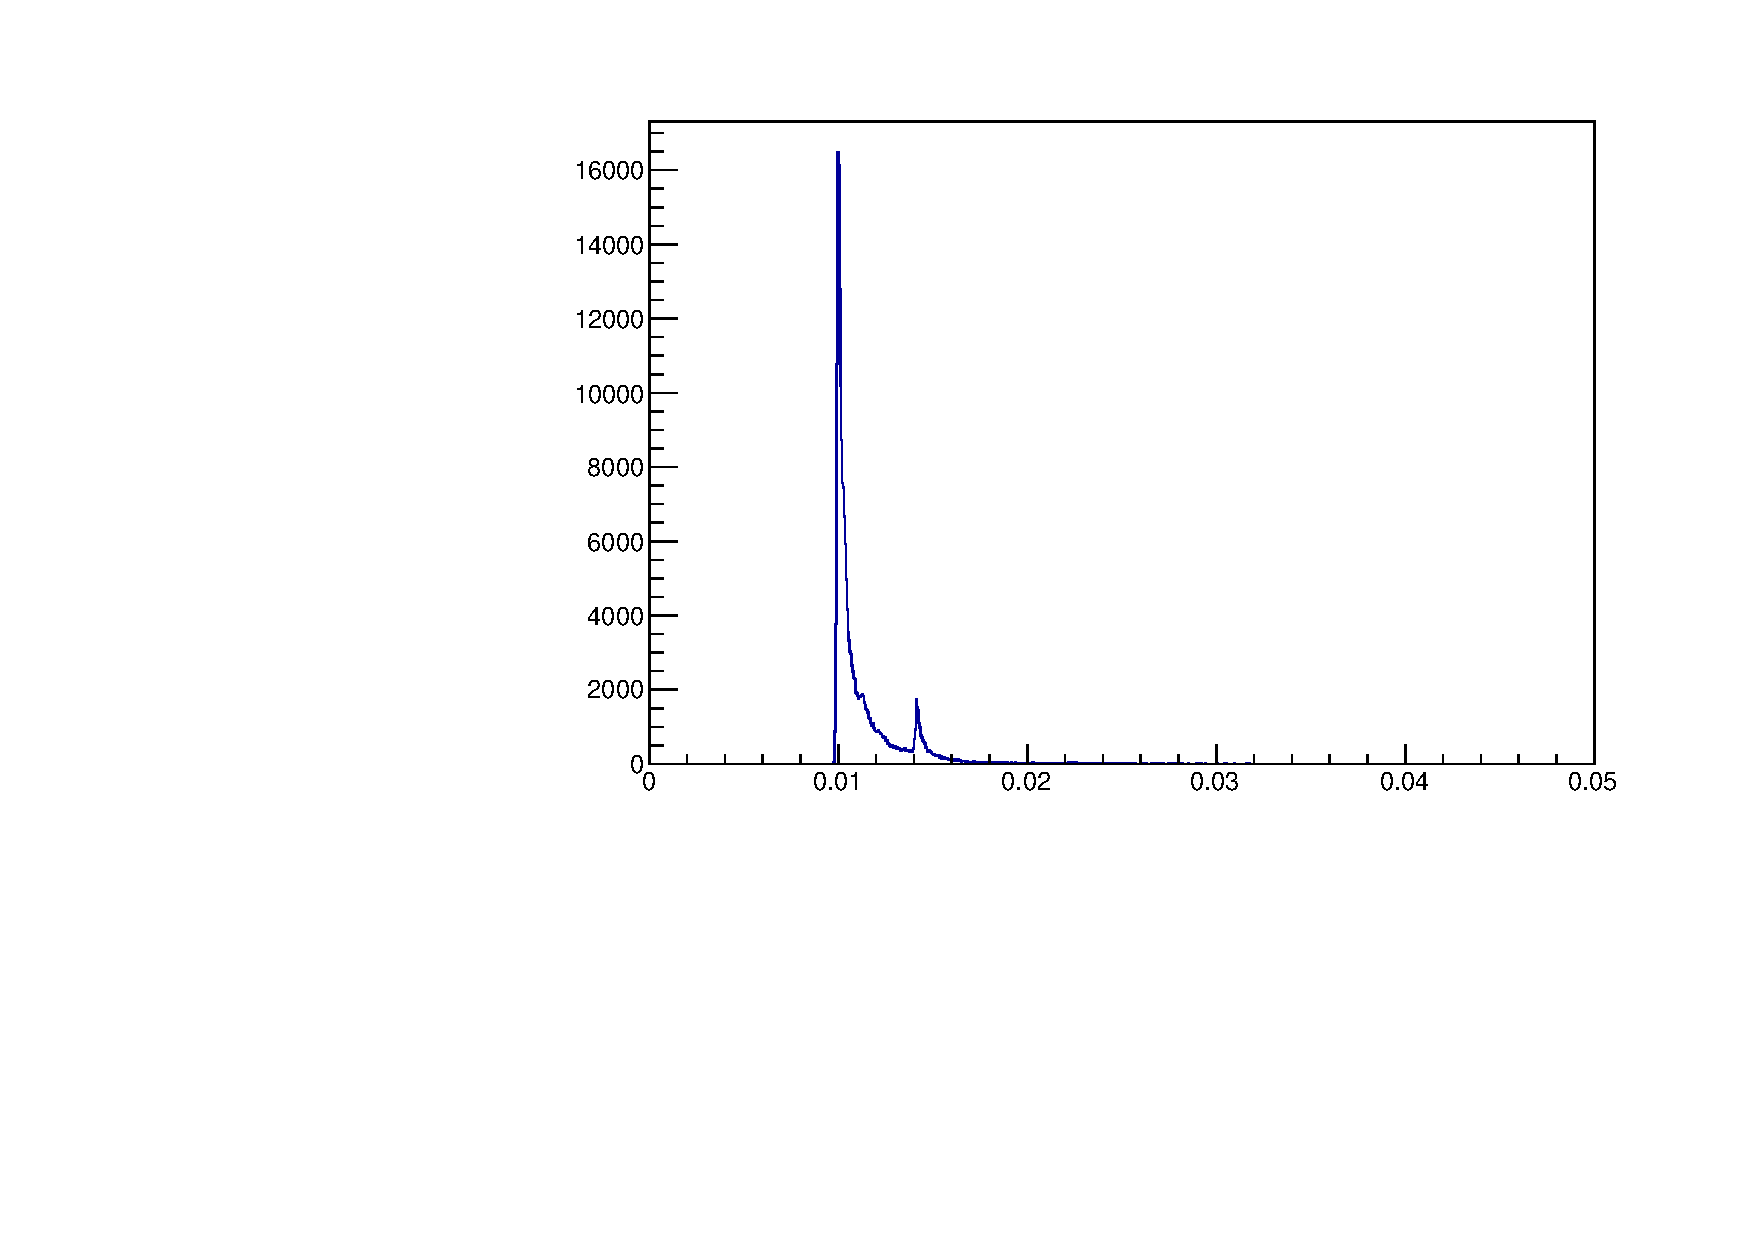
\includegraphics[width=\linewidth]{fig/nn.pdf}
	\caption{Closest neighbor distances on $P$}
\end{subfigure}%
\begin{subfigure}{.5\textwidth}
	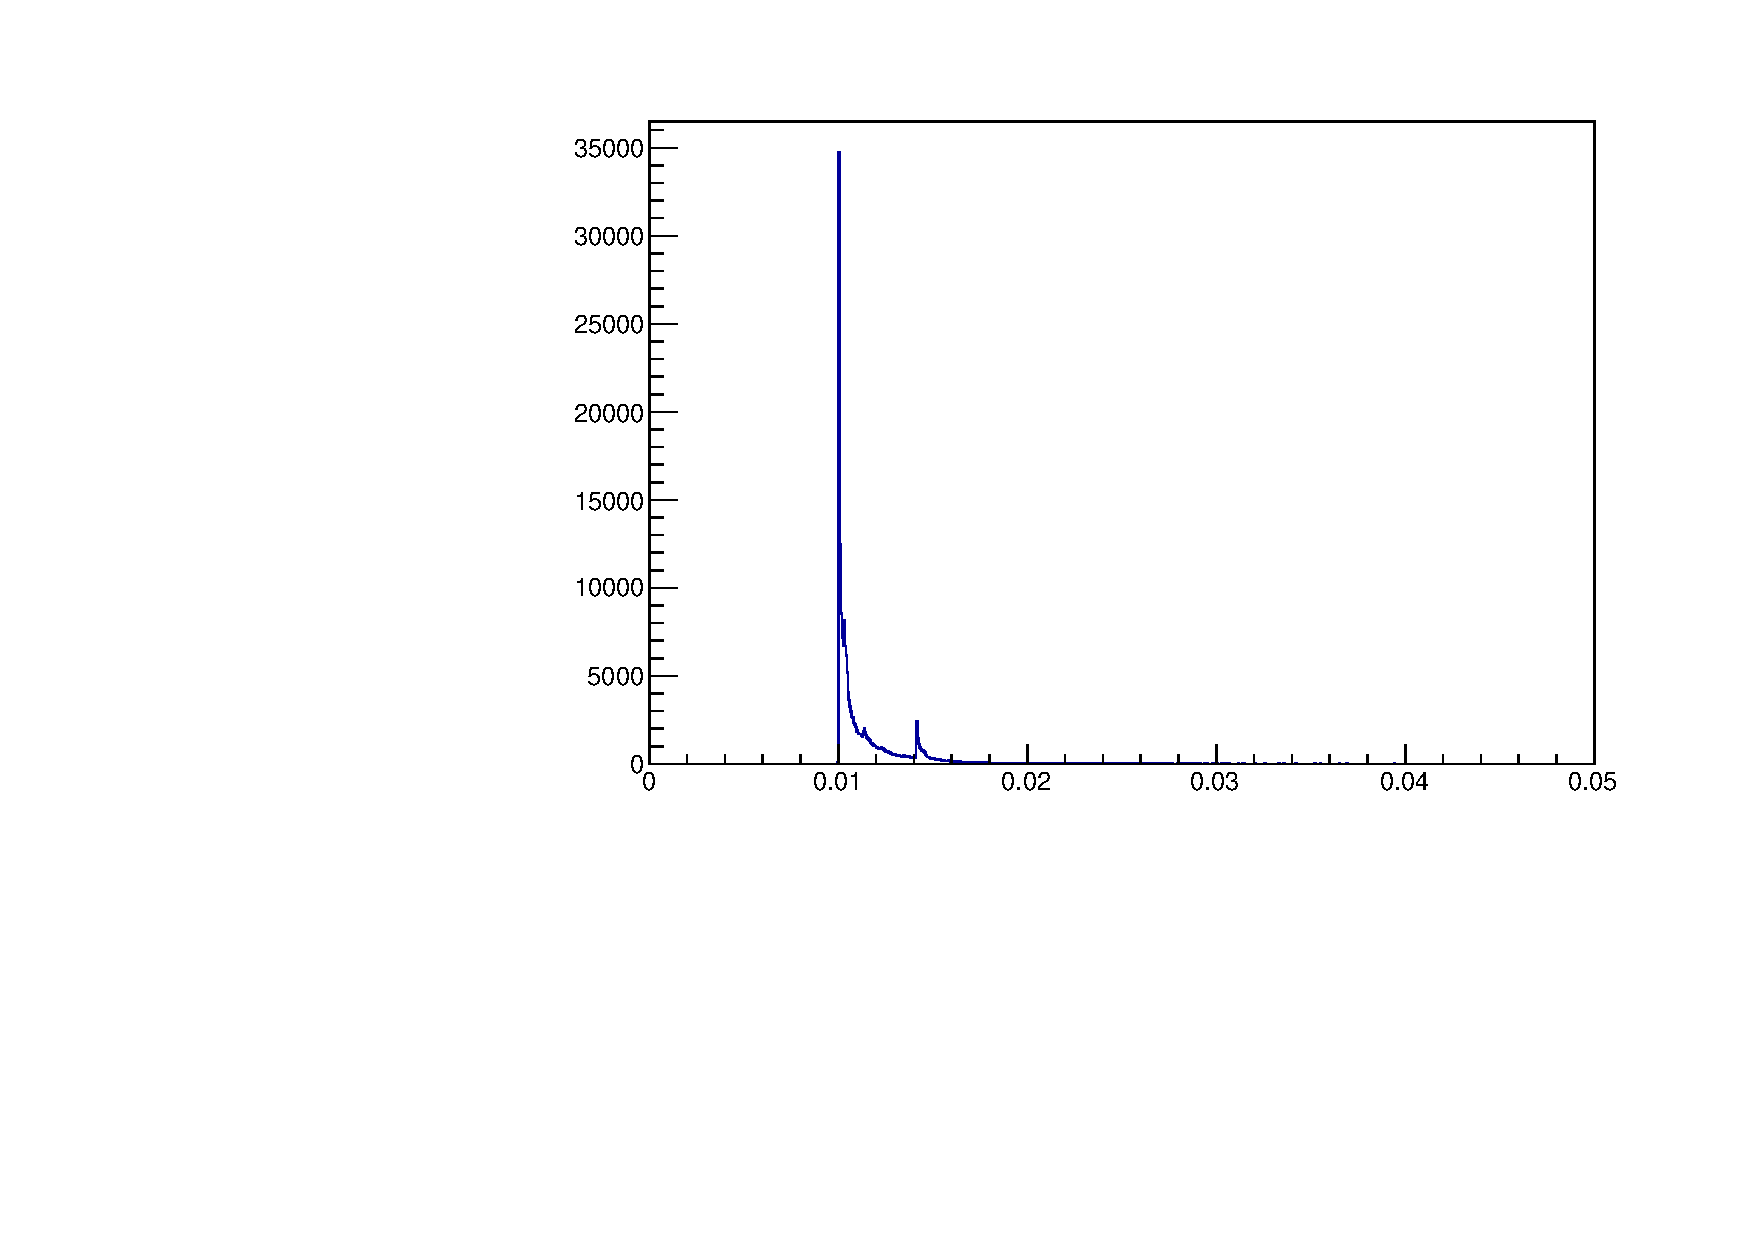
\includegraphics[width=\linewidth]{fig/nn_lmin.pdf}
	\caption{Values $l_{\text{min}}(\vec{n})$ on $P$}
\end{subfigure}	
\caption{Comparison of measured closest neighbor distances and $l_\text{min}$ values.}
\label{fig:relief_nn_hist}
\end{figure}

A similar distribution can be observed on both histograms. The spike at $0.01$ occurs because the camera is placed such that the majority of the surface is approximatively perpendicular to the rays. This confirms the correctness of the formula for $l_{\text{min}}$ for the parallelogram dispersion generated by parallel projection. The similarity of these two histograms also allows for estimation of $p_l$, even when it is not a mode.
 
The correctness of the formula for $d_{\text{max}}$ will be shown in the next section.


\subsection{Projection parameters}
If the point cloud was generated using a parallel projection camera where the graduation in the $x$ and $y$ directions on the image planes is the same, a value $p_l$ exists for the point cloud. This remains true by approximation for small extracts of large 3D scans. In the following the assumption is made that a constant value $p_l$ exists for the entire point cloud.

As shown before, using the properties of the parallelogram grid dispersion and formula \ref{eq:pargrid_lmin}, $p_l$ can be estimated by analyzing the points of the point clouds and their normal vectors. The formula is such that $l_{\text{min}}$ is proportional to $p_l$, and the proportionality constant $m = \min \left\{ \cdots \right\}$ is a function of $\vec{n}$. Assuming that the parallelogram grid covers the entire surface and that the surface is locally planar, $l_{\text{min}}$ can be computed at each point by measuring the distance to the closest neighbor in the point cloud.






\section{Own distance histogram}
Let $P$ and $Q$ be two perfectly aligned point clouds with identical surfaces, but with different point dispersions. They can differ as described in \ref{sec:registration_robostness}. $P$ is called the \emph{model}, and the points $q \in Q$ the \emph{samples}. For each sample $q \in Q$, the closest point $p \in P$ is chosen, and the distance $\|p - q\|$ is recorded. The histogram of these distances will be called the \emph{own distance histogram}. The points $p$ are chosen by the closest point criterion, without additional constraints at first.

In this section the shape of this histogram will be analyzed, and in the next section it will be compared to the \emph{cross distance histogram}, for which $P$ and $Q$ are no longer identical or perfectly aligned.

By replacing the samples $q \in Q$ with a random variable $\textbf{Q}$ with a given probability distribution, the own distance histogram can be idealized into a probability density function of the closest point distance, free of noise resulting from the sparse set of samples.

In the following, $Q$ will be taken to have a much higher point density than $P$. When the number of samples becomes infinite, the histogram converges towards the ideal probability density function. The results will later be applied to devise a method for registering high resolution with low resolution point clouds.

When used on two exact same copies of the same point clouds that are perfectly aligned, all measured distances are $0$, and so the histogram consists only of one spike.

When $P$ is artificial and its surface shape is known, $Q$ is constructed by taking a large number of points on that same surface.

\subsection{Plane with random dispersion}
Figure \ref{fig:plane_rand_d30000} shows an own distance histogram, where $P$ and $Q$ represent a single plane, and the points $p \in P$ are randomly dispersed onto it with an uniform density $\rho(P) = 30000$. For each sample $q$ the distance $d(q, P)$ to the closest point in $P$ is measured. Randomly dispersed means that the $x$ and the $y$ coordinate of each point are chosen randomly and independently, with a uniform distribution in a fixed interval.

Since $P$ and $Q$ are perfectly aligned, in this situation all distances are measured on the two-dimensional plane.

\begin{figure}[H]
\centering
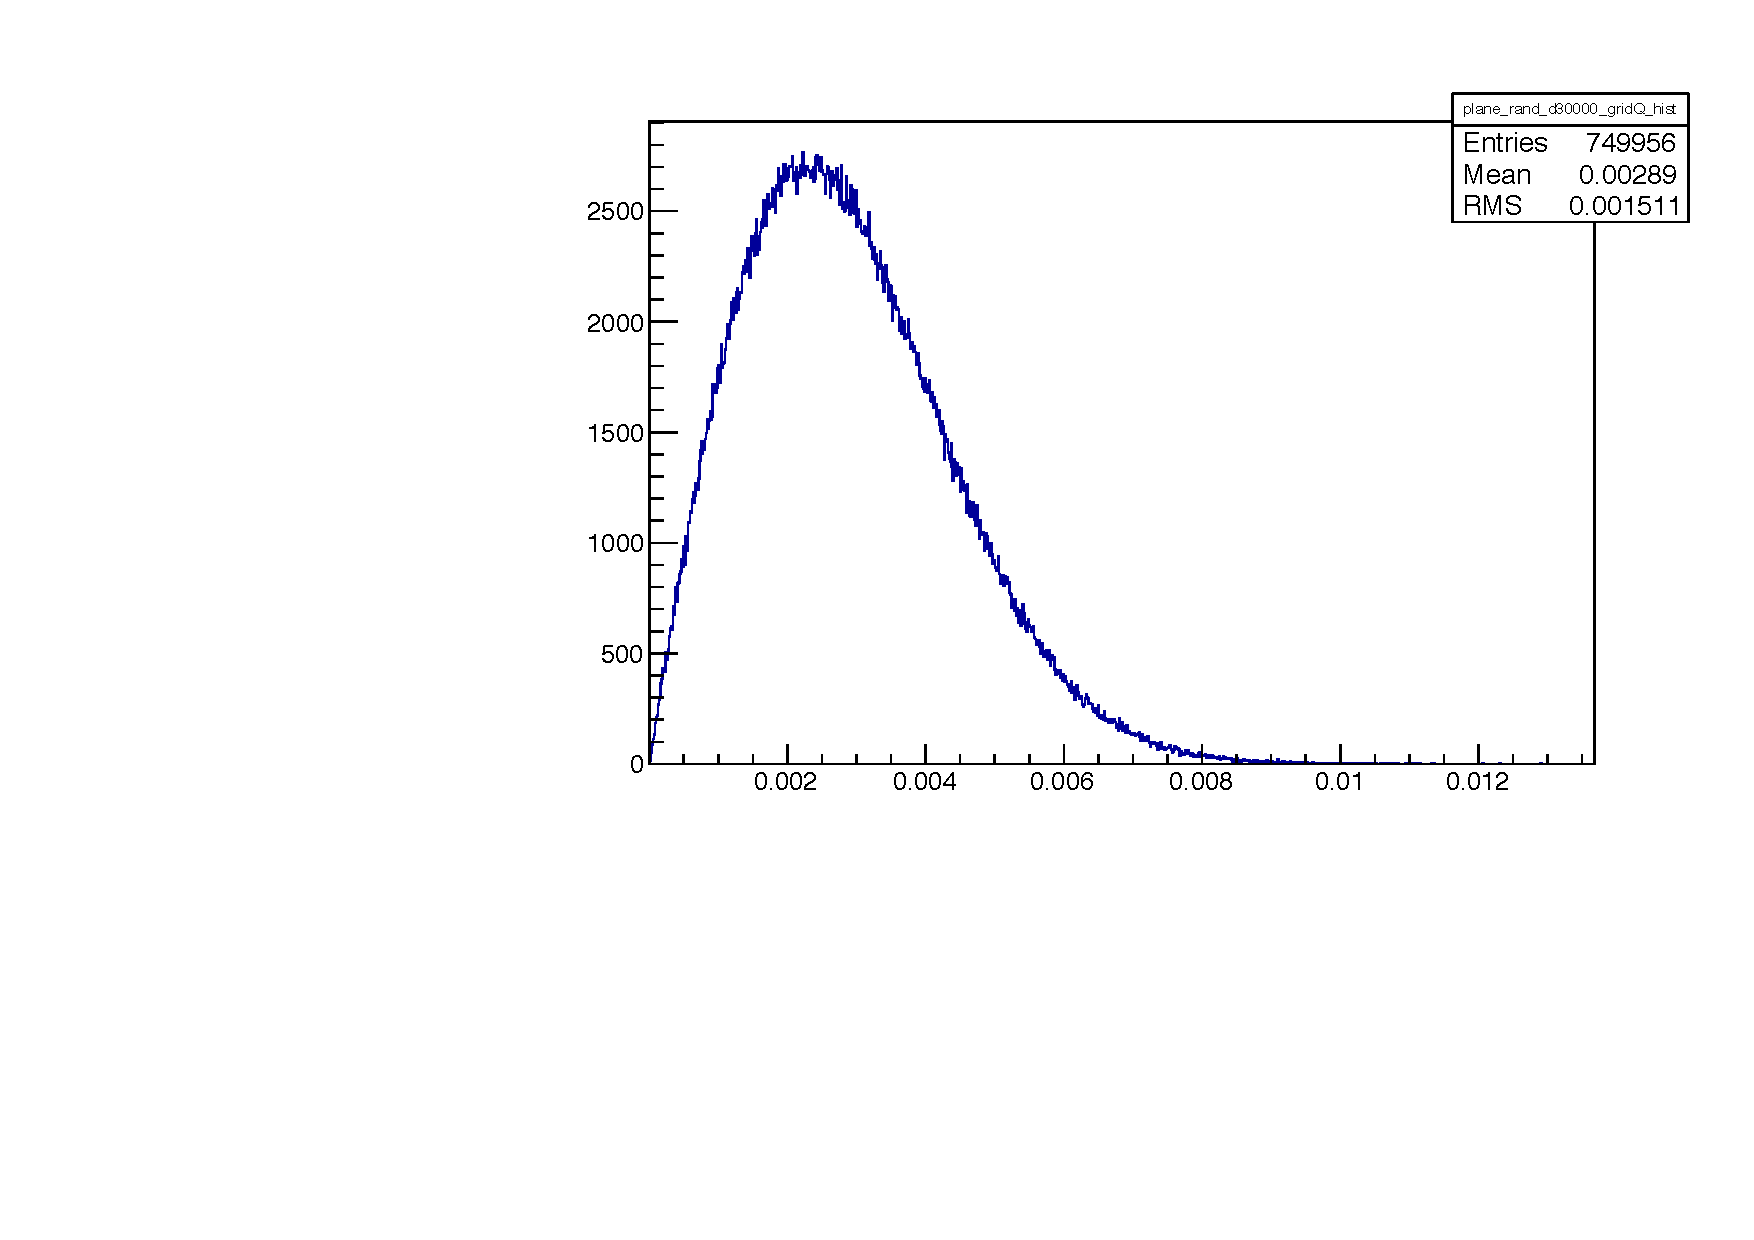
\includegraphics[width=.6\textwidth]{fig/plane_rand_d30000_gridQ.pdf}
\caption{Own distance histogram for plane $P$ with random point distribution}
\label{fig:plane_rand_d30000}
\end{figure}

Unless two points coincide, the probability at $d = 0$ is zero. It then increases, because the probability that a disk with radius $d$ around a sample point $q$ contains at least one $p \in P$ gets larger proportionally to the disk's area. But that disk must increase in radius to contain more than one point, otherwise the closest distance is the distance to the first, closer point inside the disk, and not its radius. This intuitively explains the global shape of the histogram.

The underlying probability density function $f_R$ of the random closest point distance $R$ from any point $q$ is the exponential function
\begin{equation}
f_R(r) = 2 \pi \rho(P) \, r \, e^{-\pi \rho(P) \, r^2}
\end{equation}
This formula is proven in appendix \ref{sec:proof_rand_disp_plane}. A plot is shown in figure \ref{fig:plane_rand_d}, for $\rho(P) = 30000$. It can be seen that the probability density function takes on the same shape as the histogram. By solving $\frac{\diffd}{\diffd r} f_R(r) = 0$, one obtains that the probability density function reaches its maximum at
\begin{equation}
r_{\text{mode}} = \frac{1}{\sqrt{2 \pi} \sqrt{\rho(P)}}
\end{equation}

The mean $\bar{r}$ value for the closest point distance is obtained using the integral
\begin{equation}
\bar{r} = \int_{0}^{\infty} r \, f_R(r) \, \diffd r = \frac{1}{2 \sqrt{\rho(P)}}
\end{equation}

\begin{figure}[p]
\centering
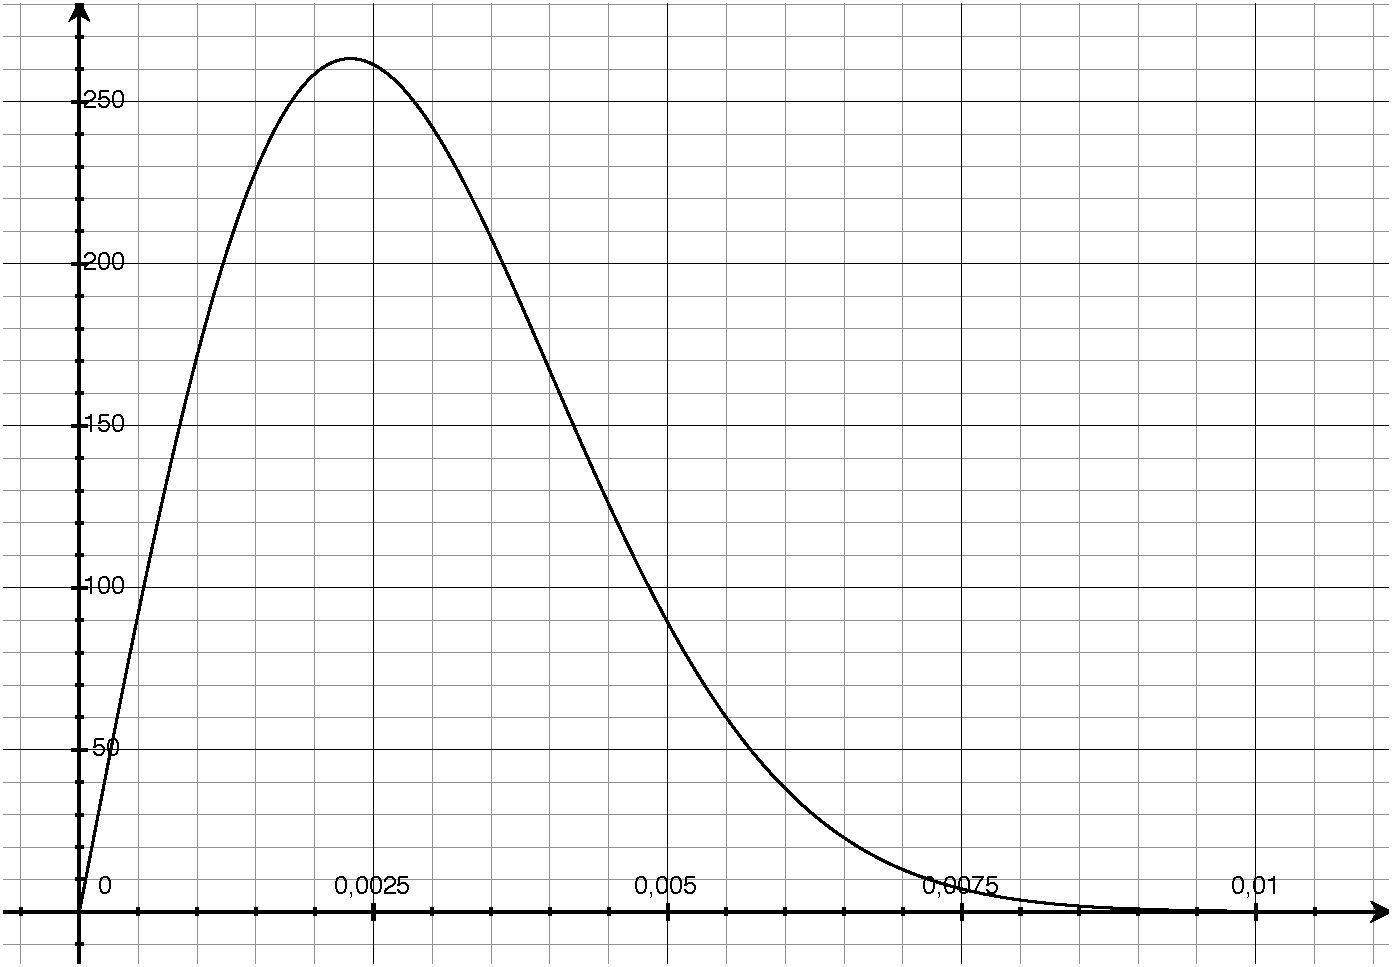
\includegraphics[width=.5\textwidth]{fig/plane_rand_d.pdf}
\caption{Probability density function of closest point distance, for plane $P$ with randomly dispersed points}
\label{fig:plane_rand_d}
\end{figure}

This random points dispersion represents the most general case, where no information about the dispersion of sample points on the surfaces is known. 



\subsection{Dispersion of sample points}
In order to obtain a histogram that closely resembles the theoretical probability density function, the dispersion of the sample points $q \in Q$ should be such that its density is much higher than that of the model points, and has a low variance. If the density is not high enough, the range of possible placements of sample points relative to surrounding model points is sampled too sparsely, leading to a low resolution histogram. If the variance is too high, some placements will be oversampled in comparison to others, and the histogram will contain more noise.

Figure \ref{fig:plane_rand_d30000_randQ} shows the same histogram, but with the sample points $q_i \in Q$ also being randomly dispersed on the plane (and a different number of samples). It is shown in appendix \ref{sec:proof_var_rand_pt_disp} that the local density is not constant.

This effect is greatly reduced when the sample points on $Q$ are instead dispersed on a regular square grid. The deviation of $N(A)$ from $\bar{N}(A)$ then occurs only due to aliasing near the border of the region $A$, so the variance is near-zero. It gets lower with a higher density of the samples $q \in Q$ and consequently lower side length of the square grid. This was used to obtain the histogram \ref{fig:plane_rand_d}.

\begin{figure}[p]
\centering
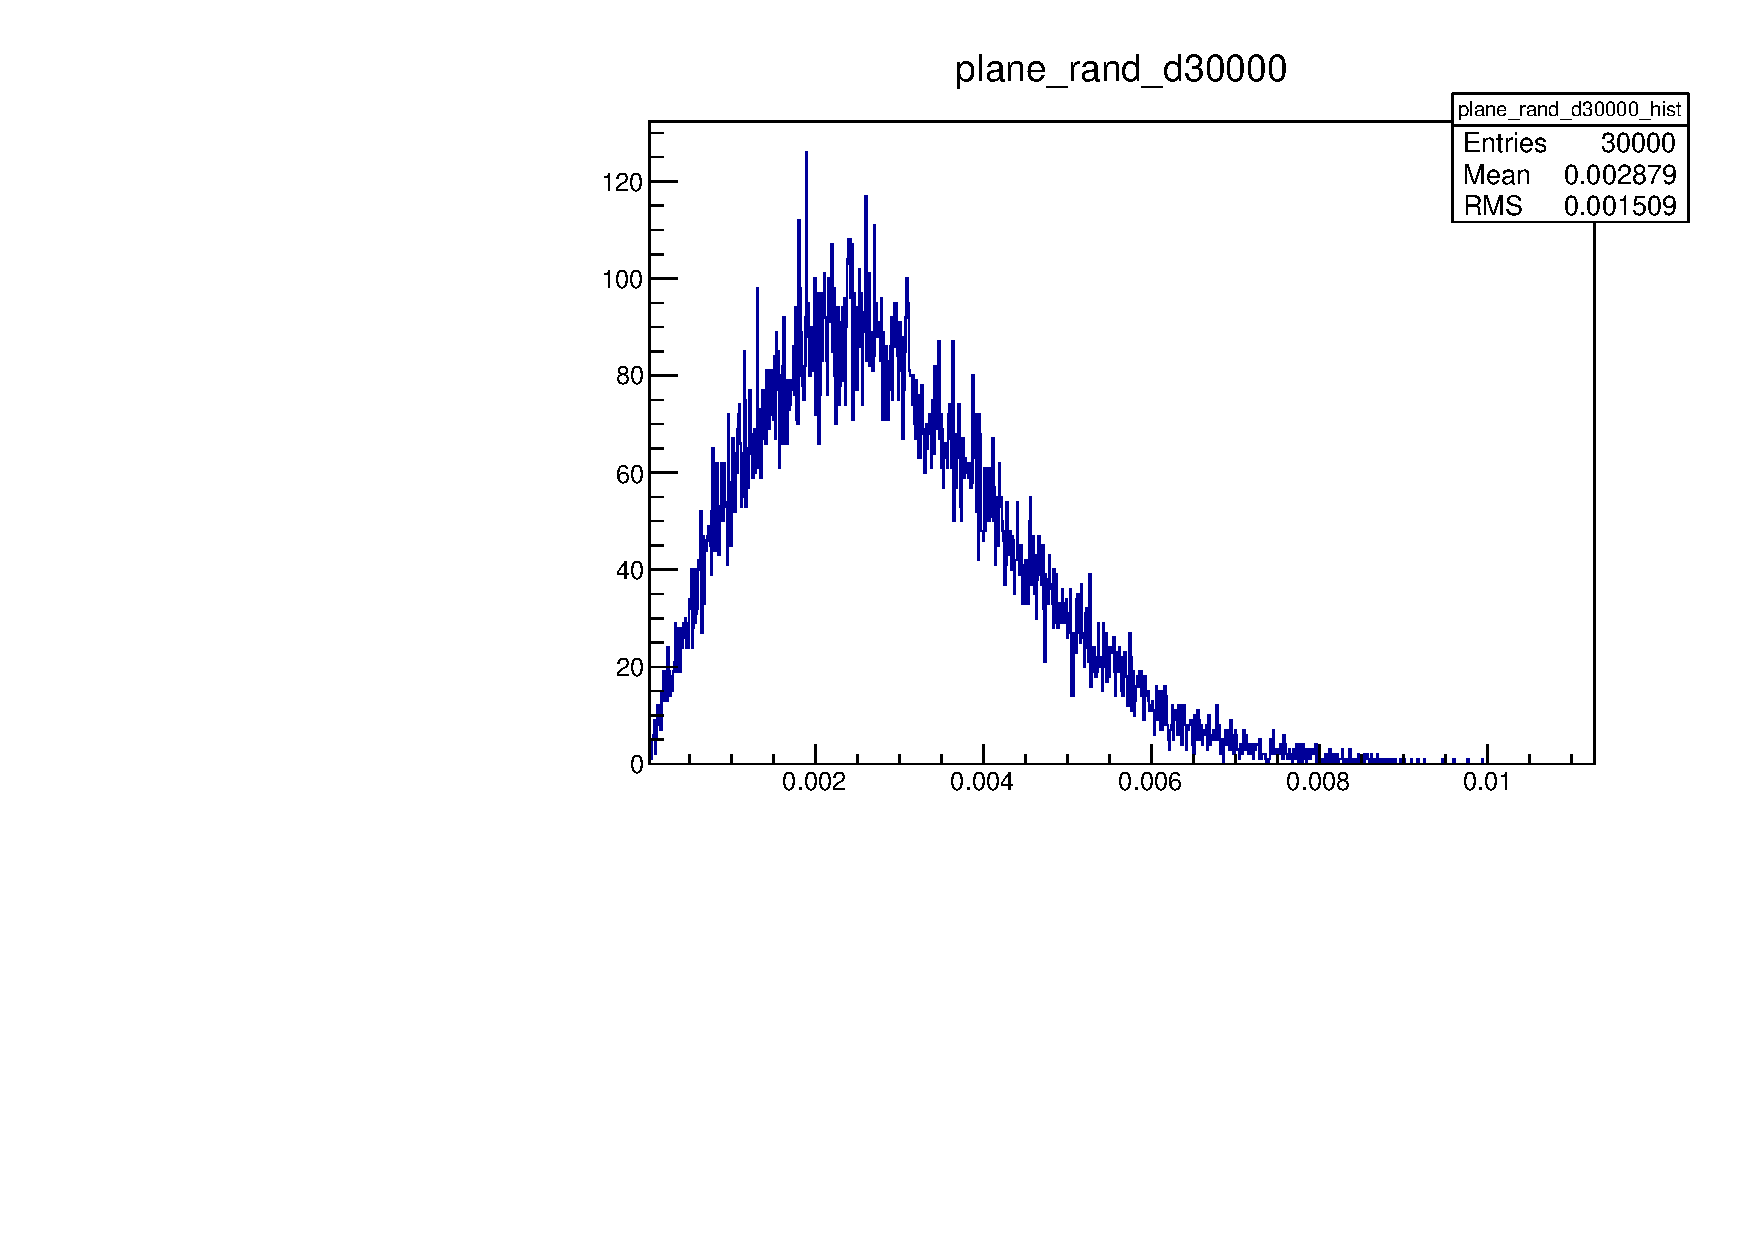
\includegraphics[width=.6\textwidth]{fig/plane_rand_d30000.pdf}
\caption{Same as figure \ref{fig:plane_rand_d30000} but with randomly dispersed samples $q \in Q$}
\label{fig:plane_rand_d30000_randQ}
\end{figure}


When working with artificially generated, perfectly aligned point clouds with a square grid point dispersion, the side lengths $l_P$ and $l_Q$ for the model and the sample point clouds must be chosen such that $\frac{l_P}{l_Q} \notin \mathbb{Q}$, otherwise same placements of sample points relative to model points will repeat, and a larger number of sample points doesn't increase histogram quality. For example if $l_P = 0.1$ and $l_Q = 0.02$, each square of the model will have $25$ sample points placed within it at the same relative positions. Taking into account that floating point numbers with limited precision are used, it means that when considering $l_P$ and $l_Q$ to be rational numbers, they should be chosen such that their least common multiple should is as high as possible.


\subsection{Plane with square grid dispersion}
Figure \ref{fig:plane_cphist} shows the distance histogram of two perfectly aligned planar surfaces $P$ and $Q$, where the points on $P$ are dispersed on a square grid. $\rho(P) = 20000$ and $30000$, respectively. The number of samples is $N(Q) = 300000$.

\begin{figure}[H]
\centering
\begin{subfigure}{.5\textwidth}
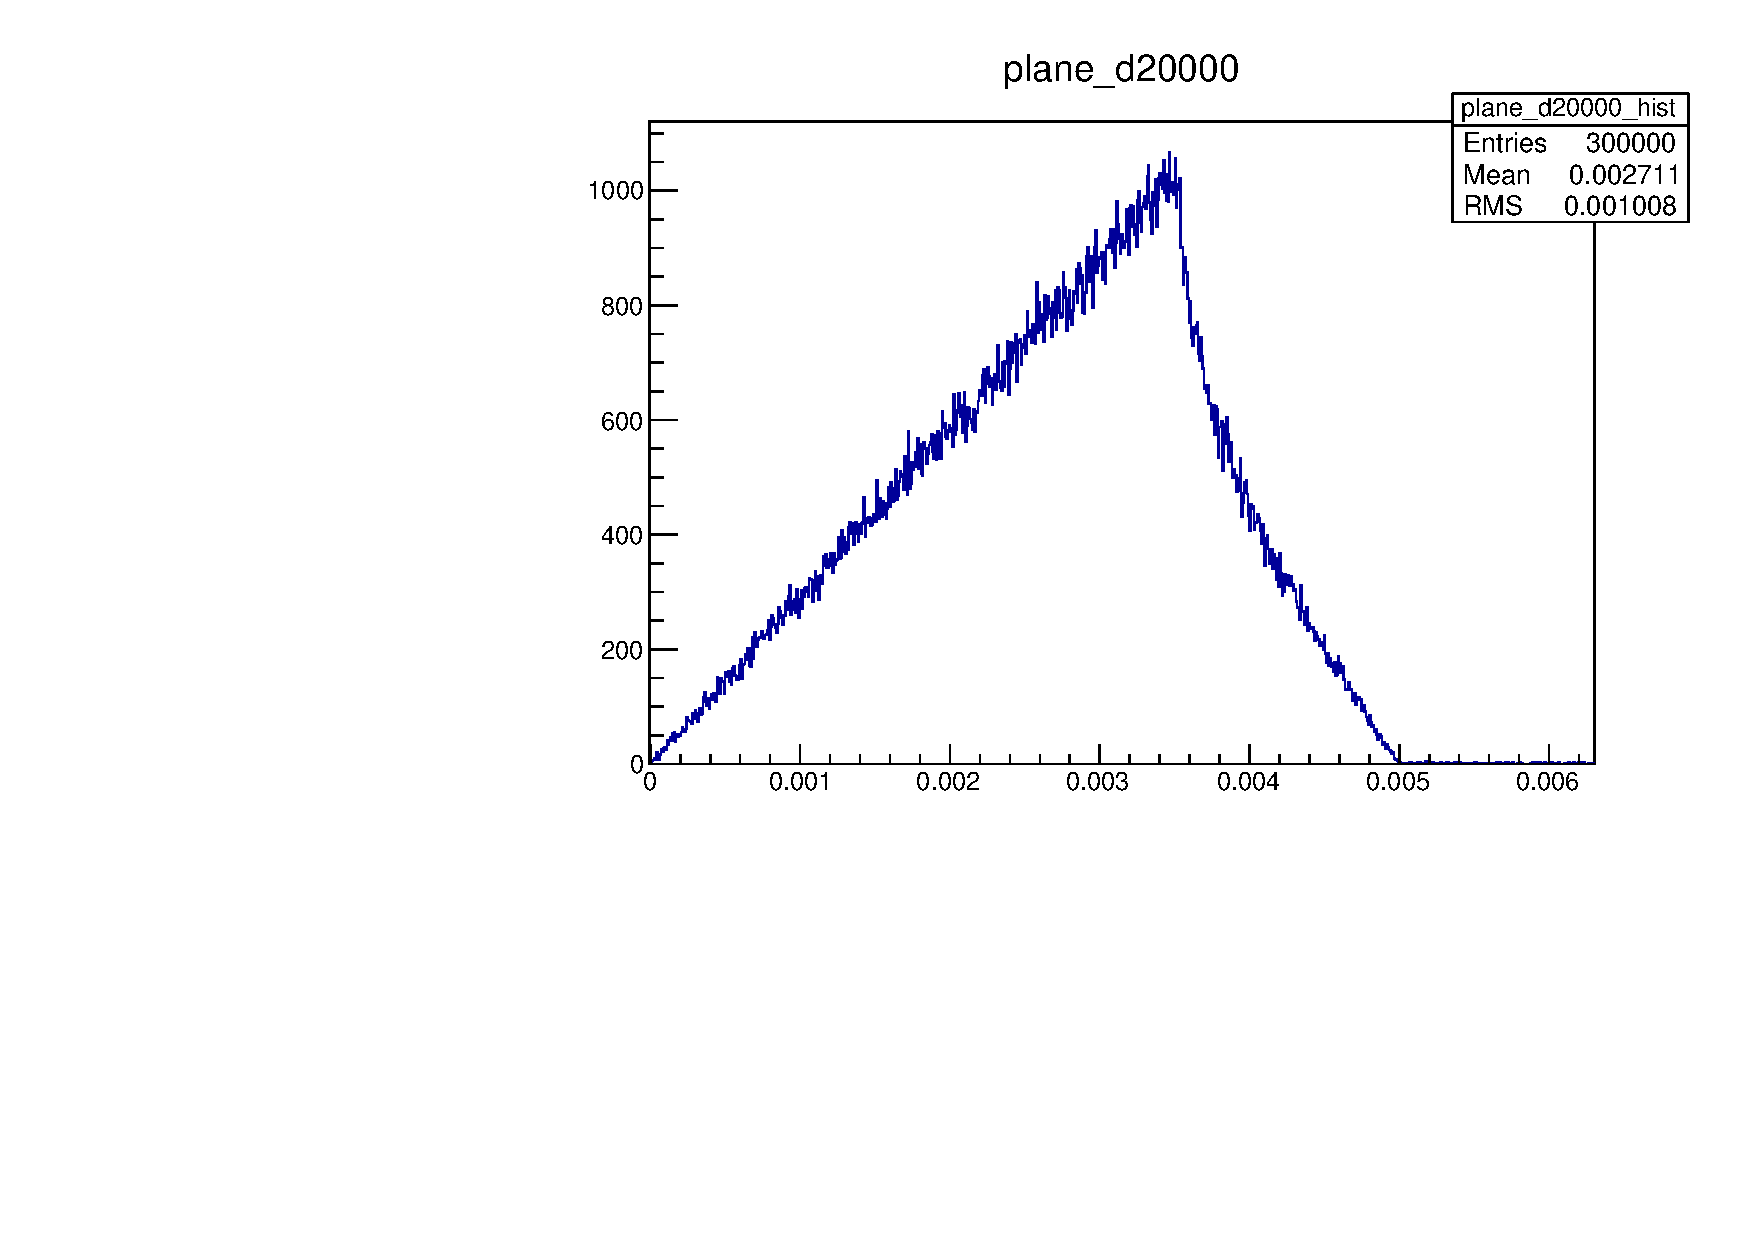
\includegraphics[width=\linewidth]{fig/plane_d20000.pdf}
\end{subfigure}%
\begin{subfigure}{.5\textwidth}
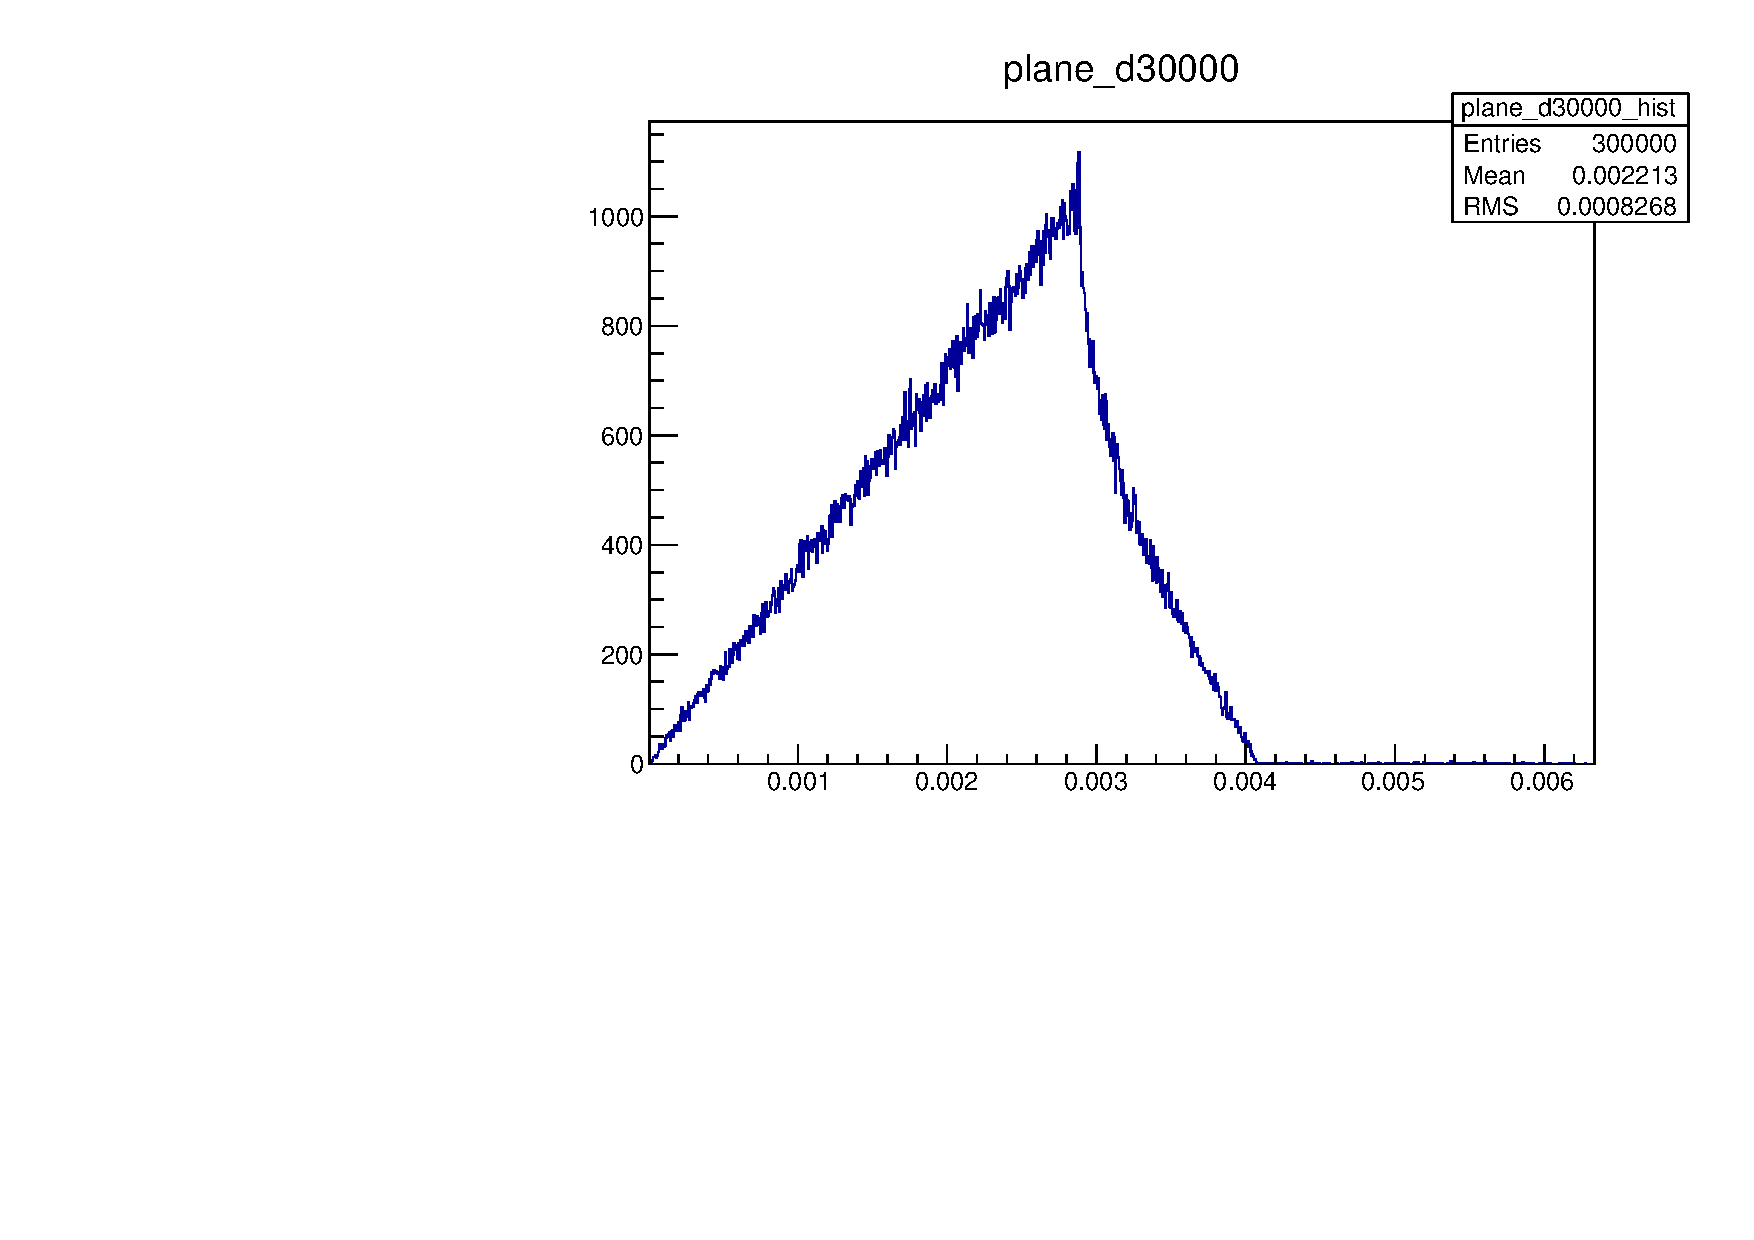
\includegraphics[width=\linewidth]{fig/plane_d30000.pdf}
\end{subfigure}
\caption{Own distance histogram for plane $P$ with square grid point dispersion}
\label{fig:plane_cphist}
\end{figure}

The probability density function $f_R$ is
\begin{equation}
f_R(r) = \frac{r}{2 l} \times \begin{cases}
	\frac{\pi}{4} & 0 \leq r \leq \frac{l}{2} \\
	\frac{\pi}{4} - \arctan{\sqrt{\left( \frac{2r}{l} \right)^2 - 1}} & \frac{l}{2} < r < \frac{l}{2} \sqrt{2}
\end{cases}
\end{equation}
with $l = \frac{1}{\sqrt{\rho(P)}}$. This is proven in appendix \ref{sec:proof_sqgrid_disp_plane}. The plot is shown in figure \ref{fig:sq_grid_d} for $l = 2$.

The probability rises linearily from $O$ to to its mode at $r = \frac{l}{2}$. Within that range, the sample point falls within the non-overlapping disks of radius $\frac{l}{2}$ around the model points. A similar characteristic linear increase exists for parallelogram grid dispersion, and for non-planar surfaces, when $P$ and $Q$ are aligned. This will be used to define a registration accuracy measure.

\begin{figure}[p]
\centering
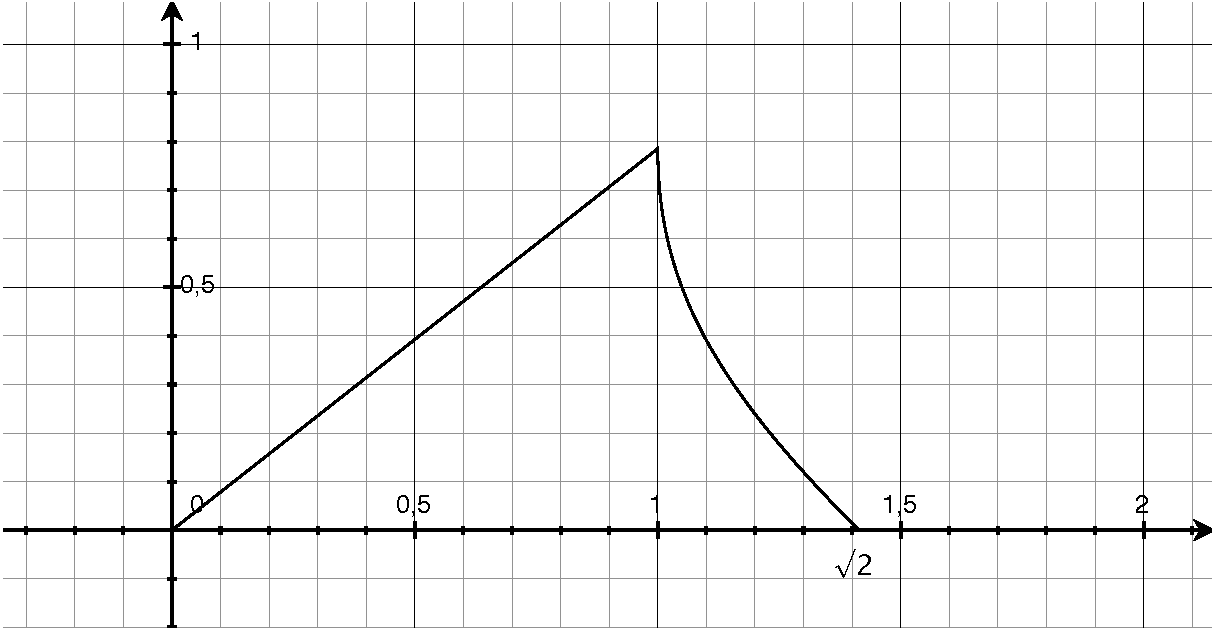
\includegraphics[width=.5\textwidth]{fig/sq_grid_d.pdf}
\caption{Probability density function of closest point distance, for plane $P$ with square grid point arrangement}
\label{fig:sq_grid_d}
\end{figure}


\subsection{Plane with parallelogram grid dispersion}
The square grid dispersion in a special case of the parallelogram grid dispersion. Figure \ref{fig:plane_par_cphist} shows an example of an own closest point histogram obtained when the model point cloud has a parallelogram grid point dispersion. As seen on figure \ref{fig:pargrid_proj}, it is the result of a parallel projection of a square grid on the camera image frame onto a plane in space with a normal vector $\vec{n}$, relative to the camera's coordinate system. For this example, $\vec{n} \approx \transpose{(-0.253023, 0.787174, -0.562438)}$, and the square grid on the image plane has a side length of $p_l = 0.067$.
s
Figure \ref{fig:par_grid} is a close-up view of the plane, showing the parallelogram grid of $P$, and the higher density square grid sample point cloud $Q$ in blue.


\begin{figure}[H]
\centering
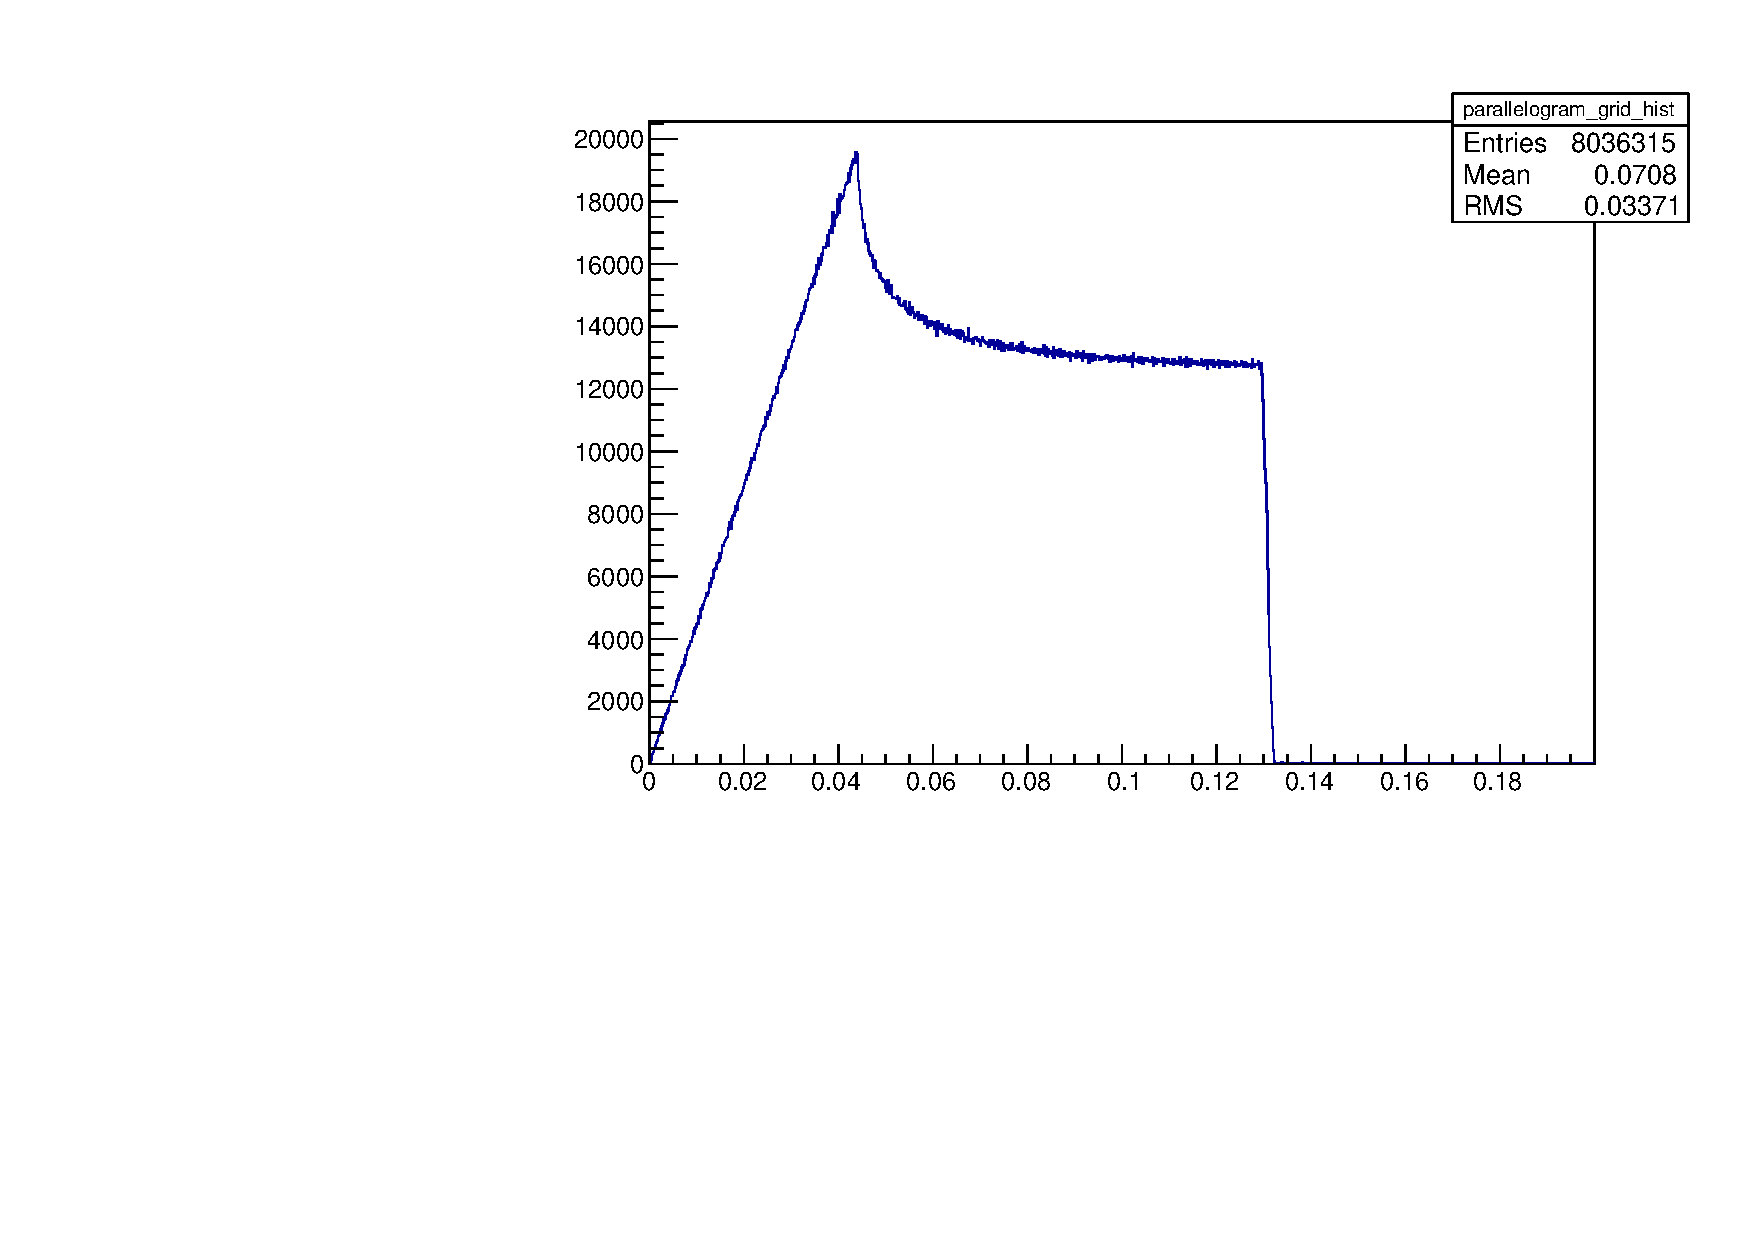
\includegraphics[width=.5\textwidth]{fig/parallelogram_grid.pdf}
\caption{Own distance histogram for plane $P$ with parallelogram grid point dispersion}
\label{fig:plane_par_cphist}
\end{figure}

It can be seen that the histogram's underlying probability density function is again a piecewise function, and that its first segment is still a linear increase from the zero point to the mode of the histogram.

Using a similar argument as for the square grid dispersion, one can show that the linear increase happens from $0$ to $\frac{1}{2} l_\text{min}$. Applying the formula \ref{eq:pargrid_lmin} developed in the previous section, a value of approximatively $0.0441$ is found for this example. It corresponds to the mode seen on the histogram.

\begin{figure}[p]
\centering
{
	\setlength{\fboxsep}{0pt}%
	\setlength{\fboxrule}{0.5pt}%
	\fbox{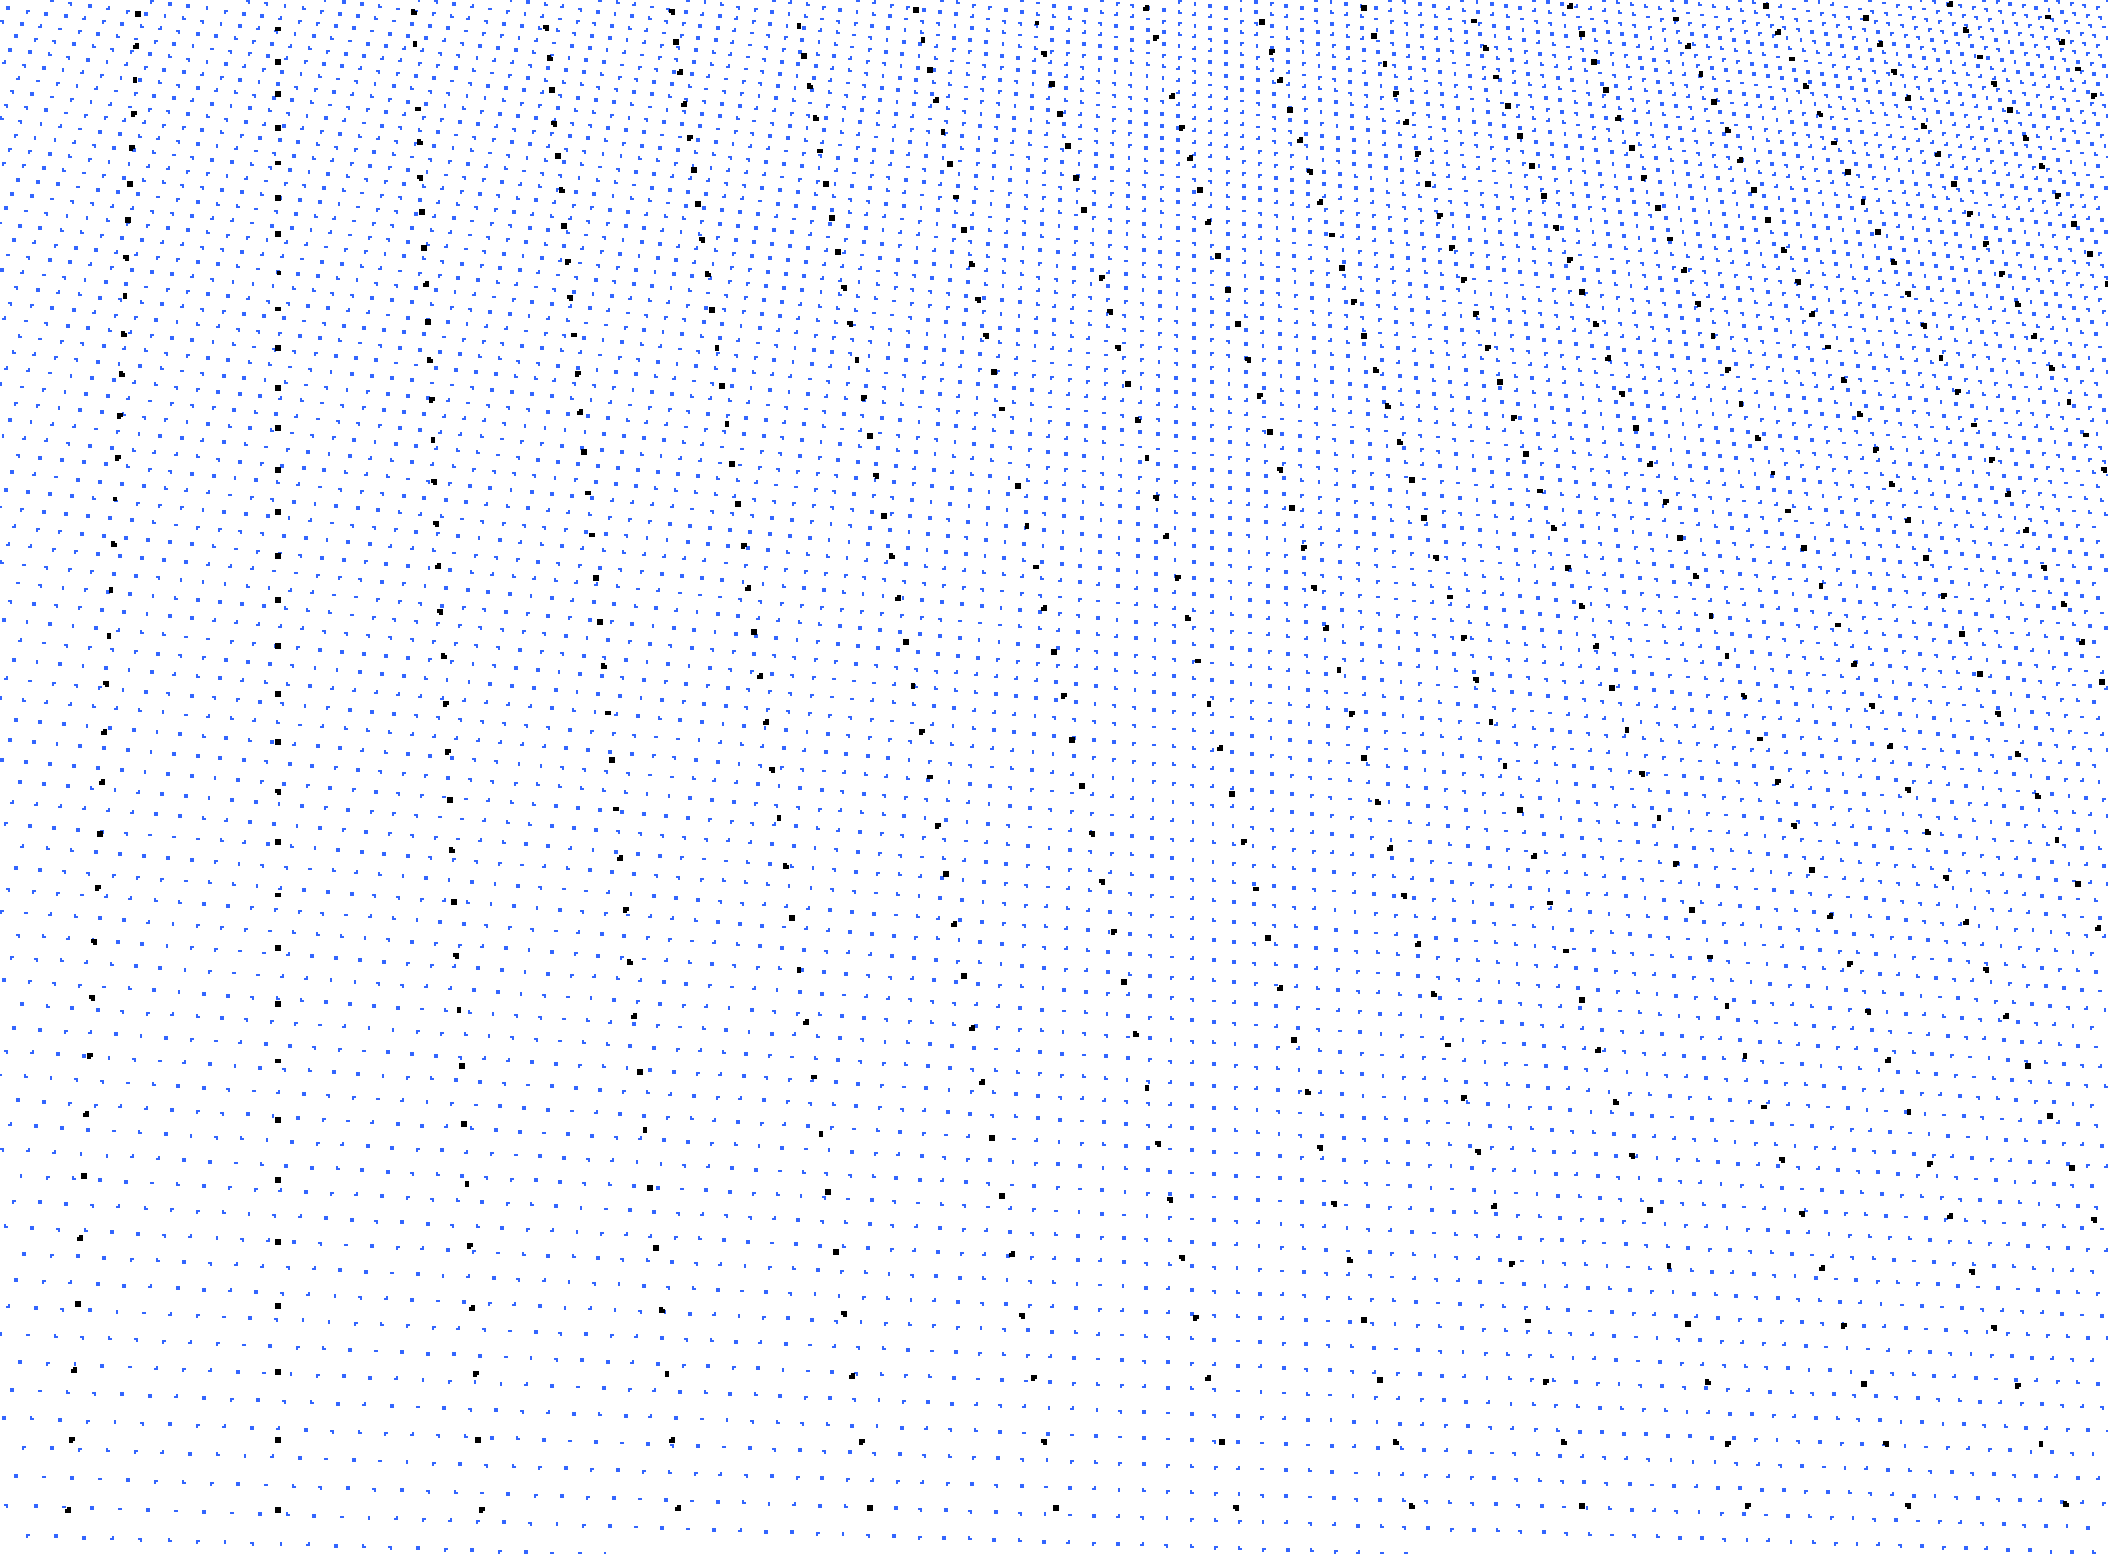
\includegraphics[width=.5\textwidth]{fig/closeup_pargrid.png}}%
}
\caption{Close-up view of parallelogram grid in $P$ (black), and sample point cloud $Q$ (blue)}
\label{fig:par_grid}
\end{figure}


\subsection{Adjusted own distance histogram}
This implies that it is possible to calculate the range of the first, linearly increasing segment of the histogram, using only the plane's normal vector $\vec{n}$ and the side length $p_l$ of the parallel projection camera. Here an attempt is made to use this result to product an \emph{adjusted own distance histogram}, which still has the initial linear increase, for point clouds that are not planes.

When the surface is no longer a plane, $\vec{n}$ will no longer be constant, but can have a different value for each point. However for smooth surfaces on the model, the normal vector will remain approximatively constant on local regions of neighboring points, as can be seen on the close-up views in the previous sections. On these planar regions the parallelogram grid point dispersion appears.

Under the assumption that most of the point clouds consists of such planar regions, its own distance histogram will be a superposition of the kinds of parallelogram grid histograms seen before, with an initial linear increasing segment.

\subsubsection{Multi-planes point cloud}
In order to test the shape of this superposition histogram, an artificially generated ``multi-planes'' point cloud is used. It consists of multiple planes places randomly in space at different orientations, projected using a parallel projection camera. An example with two planes is shown in figure \ref{fig:disks1}, shown with decreased point density.

The two planes are bounded to the shapes of disks. This does not have an effect of the histograms, and just makes the point cloud easier to visualize. If the bound was a square, it would change depending on the rotation of the plane on its own axis.

Both planes have the parallelogram grid point dispersion. The example is chosen so that one plane is approximatively facing the camera while the other is more oblique, and has a lower $\rho$ and higher $l_\text{min}$ as a result. Figure \ref{fig:multiplane_cphist} shows the own distance histograms for the two individual planes, and the superposition histogram for the entire multi-planes point cloud.

\begin{figure}[H]
\centering
\begin{subfigure}{.32\textwidth}
	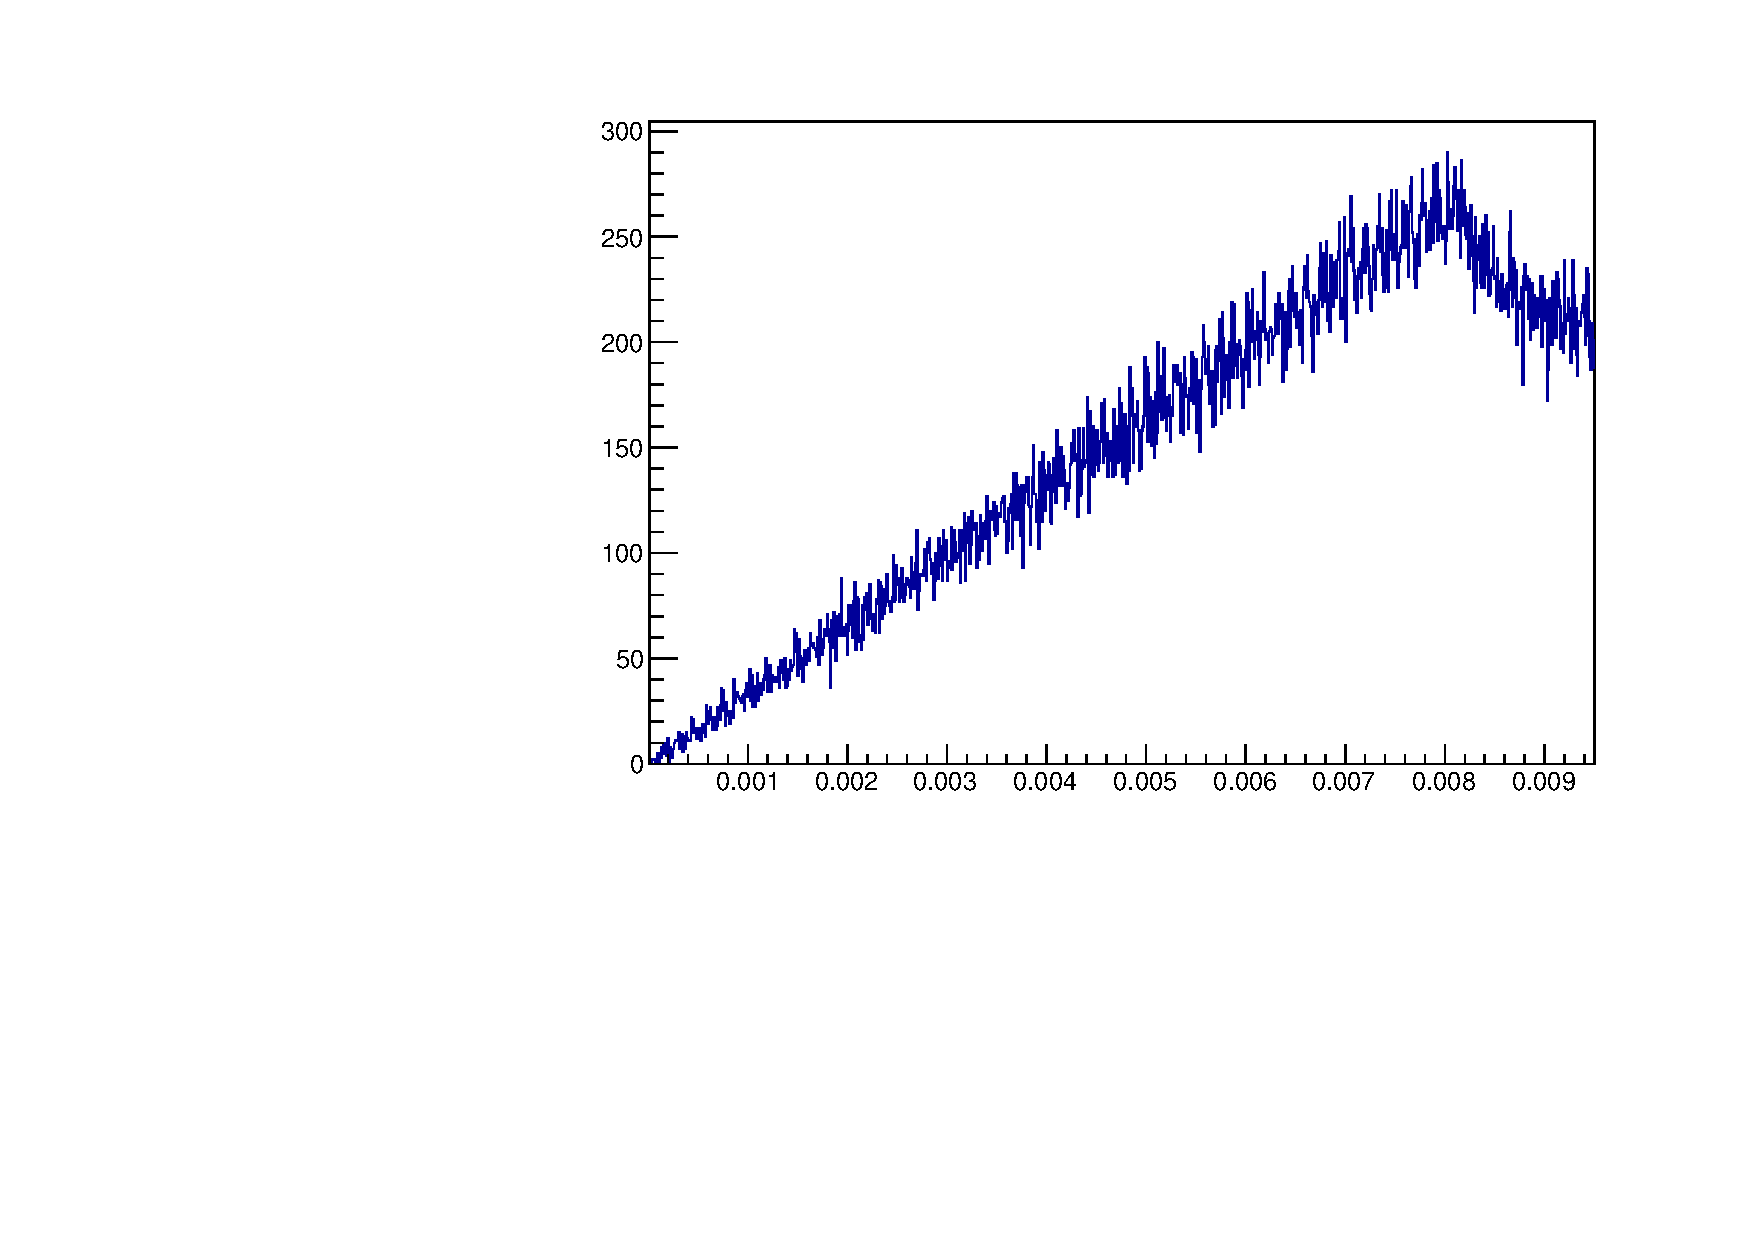
\includegraphics[width=\linewidth]{fig/orig_plane1.pdf}
	\caption{Oblique plane}
\end{subfigure}%
\begin{subfigure}{.32\textwidth}
	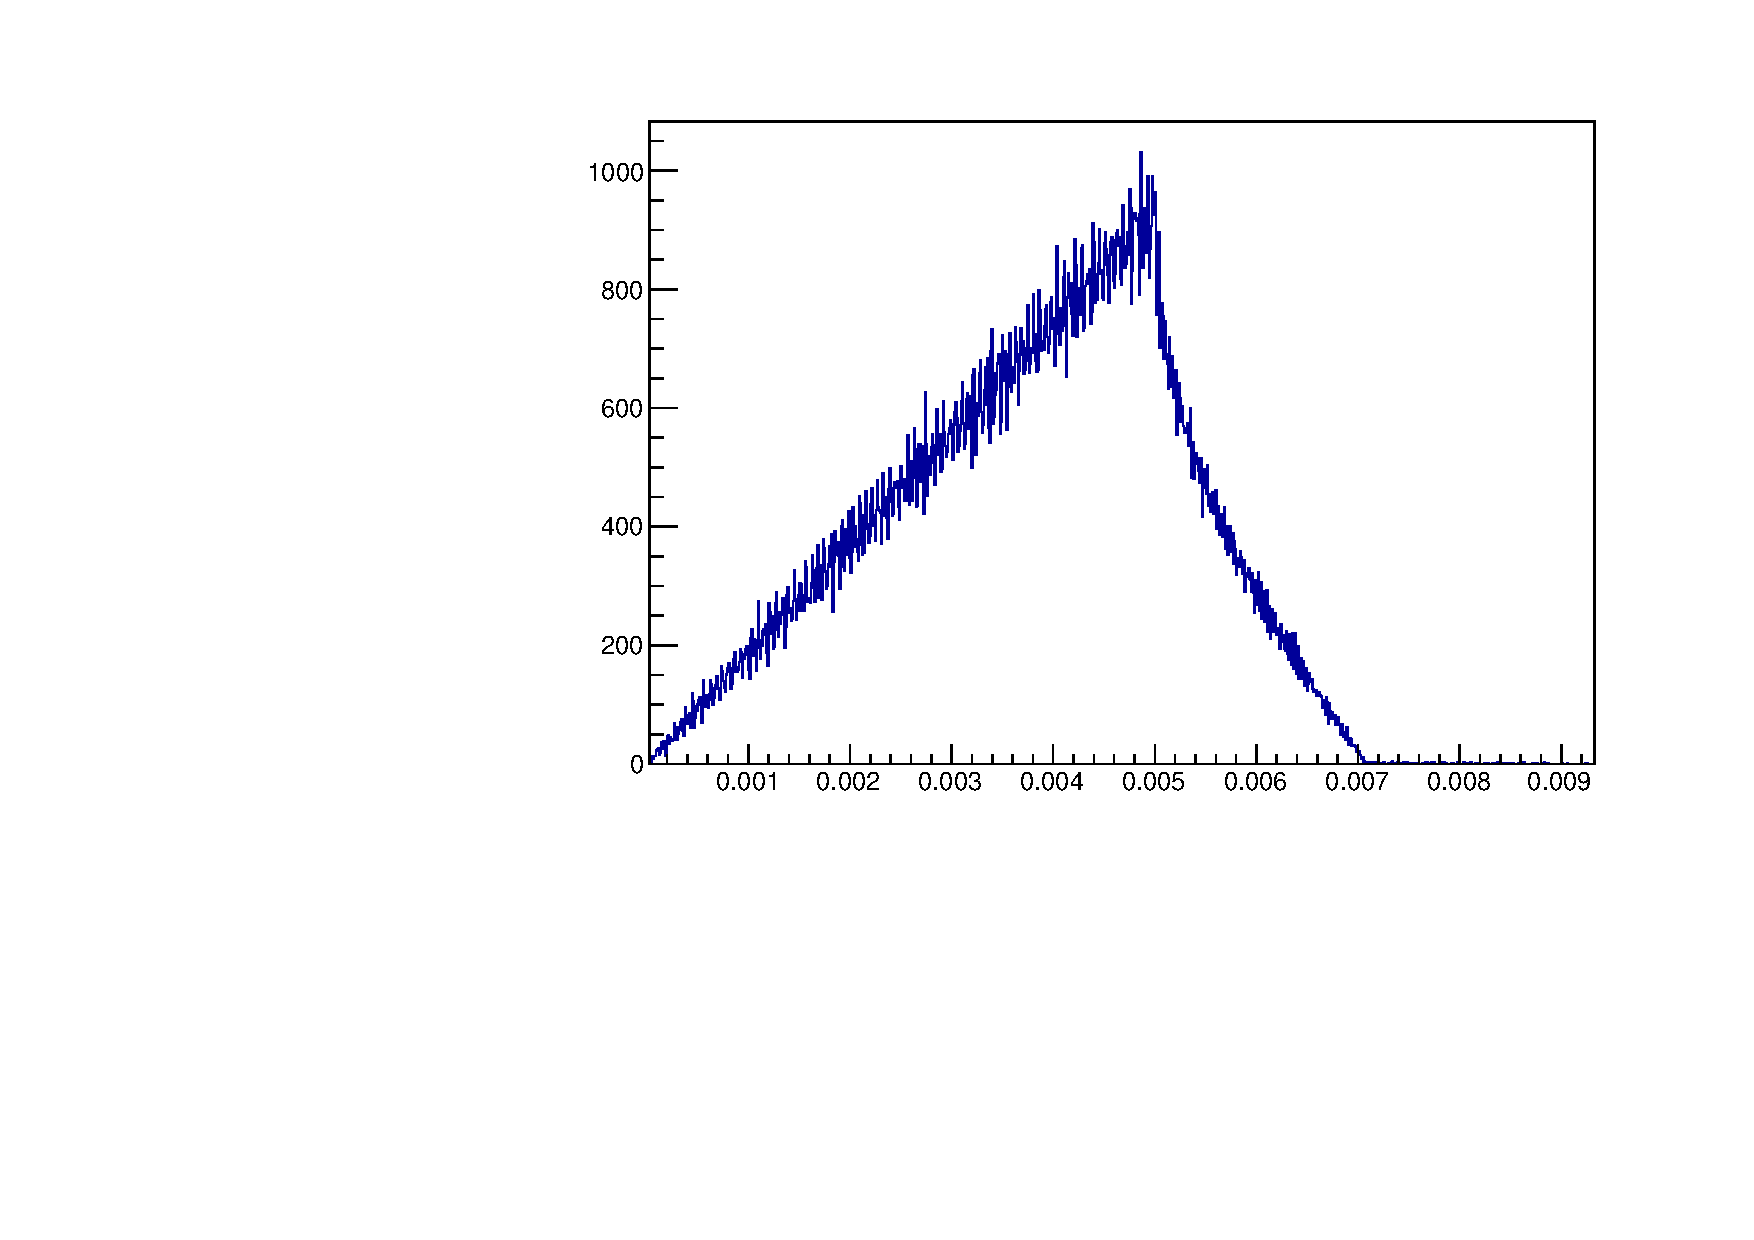
\includegraphics[width=\linewidth]{fig/orig_plane2.pdf}
	\caption{Parallel plane}
\end{subfigure}%
\begin{subfigure}{.32\textwidth}
	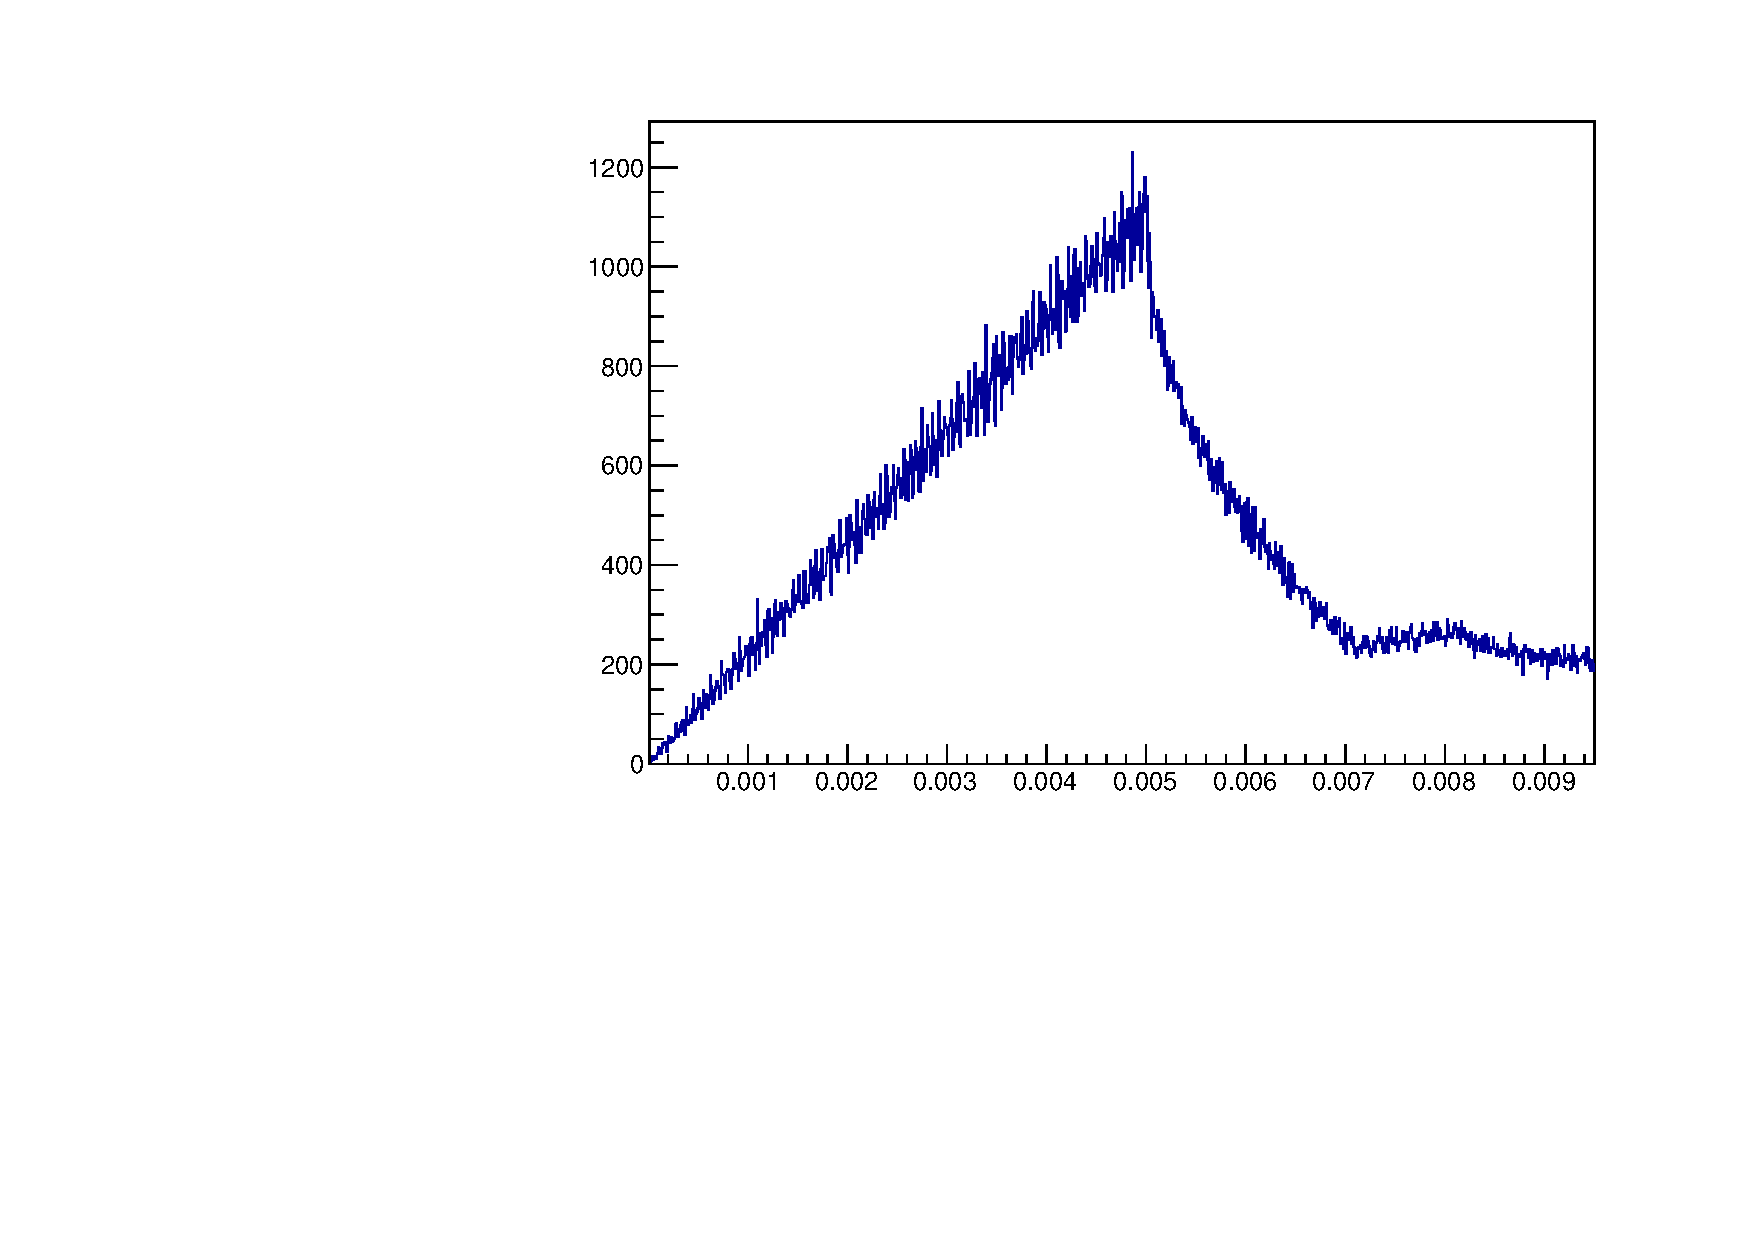
\includegraphics[width=\linewidth]{fig/orig_superposition.pdf}
	\caption{Superposition}
\end{subfigure}
\caption{Own distance histogram for disks point cloud $P$ (individual planes, and superposition)}
\end{figure}

It can be seen that the linear segment of the superposition histogram ranges up to about $0.005$, which is the minimum of the ranges on the two individual histograms. Thus the information from the remaining linear range of the oblique plane is lost.

The adjusted own distance histogram is created as follows: For each $q \in Q$, the closest point $p \in P$ is taken, for which $d = \|p - q\|$ is minimal. Then instead of $d$, the value $\frac{d}{l_{\text{min}}(\vec{n})}$ is recorded in the histogram, with a weight of $\frac{1}{\rho(\vec{n})}$.


\begin{figure}[p]
\centering
{
	\setlength{\fboxsep}{0pt}%
	\setlength{\fboxrule}{0.5pt}%
	\fbox{
\includegraphics[width=.5\textwidth]{fig/disks1.png}}%
}
\caption{Example of multi-plane point cloud}
\label{fig:disks1}
\end{figure}

\label{fig:multiplane_cphist}
\end{figure}




\subsection{Occlusion and different bounds}
Up until now $P$ and $Q$ were considered to be perfectly aligned, constitute the same surfaces, and both have points dispersed on the whole surface at an uniform distribution. On point clouds obtained from real 3D scans this last constraint is no longer true: Parts of the surface will be occluded, and two point clouds will have different bounds.

When part of the sample point cloud $Q$ are removed



\section{Cross distance histogram}


\section{High-low density registration}
When attempting to register a short-range scan of a relatively small object with the same object in a long-range scan, the short-range point cloud will have a much higher resolution. But fine registration algorithms generally make the assumption that the two point clouds have similar resolutions. The issue of registering point clouds with different resolutions seems to be largely ignored in the literature about point cloud registration algorithms.

\subsection{First experiment}
A first observation is that in general for ICP, lowering the resolution of the loose point cloud does not much reduce the accuracy of the registrations. This is shown in experiment \ref{sec:ex_bunny_hilo} (see appendix), in which the Stanford Bunny model is fine registered with a lower density copy of itself. Let $P$ be the fixed point cloud and $Q$ the (downsampled) loose point cloud.

The most basic variant of ICP is used: All points are selected, correspondences from are taken $Q$ to $P$ by the closest point criterion, no correspondences are rejected, weights are uniform, and the point-to-point error metric is used. The copies are made in such a way that they never have two points in common: $P$ is constructed by taking randomly chosen $50\%$ of the points from the original model, and $Q$ is constructed from the remaining $50\%$. After this $Q$ is randomly downsampled by $60$ different amounts.

The experiment is done in three instances. For the first one (figure \ref{fig:bunny_globmin}), $P$ and $Q$ start out perfectly aligned, and for the two other ones (figures \ref{fig:bunny_globsmall} and (figure \ref{fig:bunny_globmed})), they start out with a small (or larger) random initial transformation. $40$ iterations of the registration algorithm are run and the final errors are recorded.

The plots show the error measured using the mean unsigned distances of the true correspondences, as defined in section \ref{sec:lm_known_ttrans}. It is zero if and only if $P$ and $Q$ are perfectly aligned. The X axis indicates the ratio of the number of points $\frac{\|Q\|}{\|P\|}$.


\subsubsection{Analysis}
Two things can be observed: The final error does not depend much on the downsampling level, and the error always converges to about $0.001$, even when $P$ and $Q$ were perfectly aligned to start with.

To define a rigid transformation, three pairs of corresponding points are sufficient as long as the three points do not lie on the same plane. (see section \ref{sec:lsq_align}) So even when $Q$ is reduced to three points the point-to-point error metric can be minimized. RANSAC-based approaches to registration, such as 4PCS are based on this.

Figure \ref{ref:bunny_hilo_ev} shows how the true error evolves during the $40$ executions of ICP on the first experiment without initial displacement. $P$ and $Q$ were generated to have no common points. When choosing the points closest to the true corresponding point instead, the error does not cancel out completely, and thus the correct alignment is no longer the global minimum of the error metric.

Figure \ref{bunny_first_tcor} shows the state after the registration. $Q$ is rendered in blue color and $P$ in red. From each point $q_i \in Q$ a line segment towards the true corresponding point $q'_i$ is shown, which is not a point $p_i \in P$. On this part $Q$ has from the correct alignment deviated towards the right.

\begin{figure}[p]
\centering
{
	\setlength{\fboxsep}{0pt}%
	\setlength{\fboxrule}{0.5pt}%
	\fbox{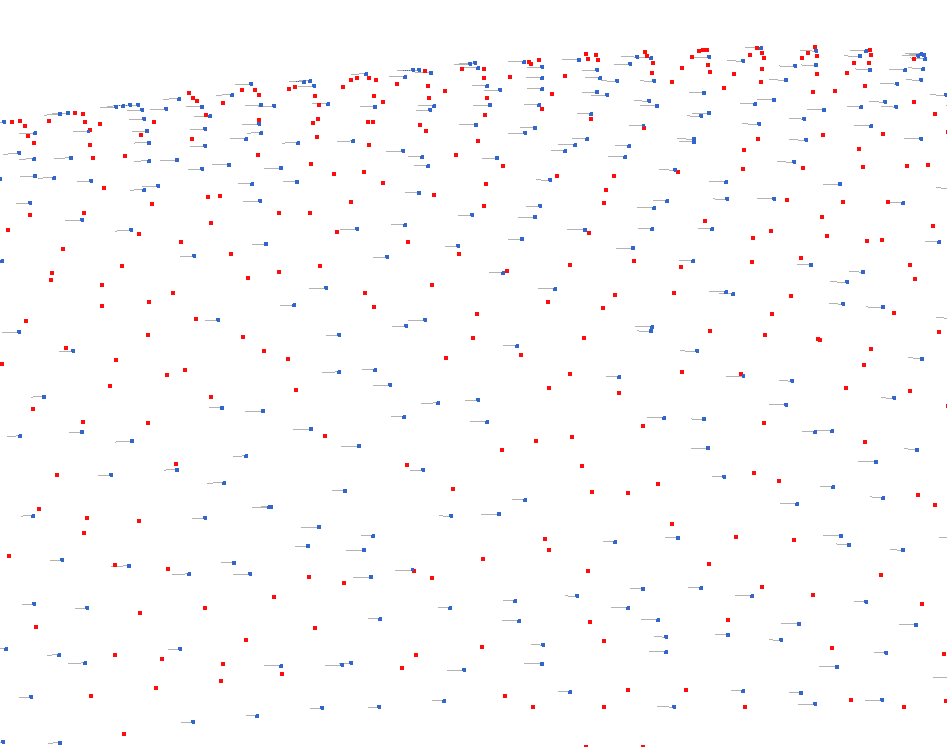
\includegraphics[width=.7\textwidth]{fig/bunny_first_tcor.png}}
}
\caption{Bunny model registered to itself, true correspondences shown}
\label{fig:bunny_first_tcor}
\end{figure}

When $\forall q_i, p_i = q'_i$, the correct alignment would be found. When $P$ and $Q$ are already aligned, $q_i = q'_i$. Figure \ref{fig:bunny_fexp_before} shows the histogram of $\|q'_i - p_i\| = \|q_i - p_i\|$ for the case when $50\%$ (or $80\%$) of the model points are taken for $P$ and the remaining for $Q$, and no additional downsampling is applied.

\begin{figure}[h]
\centering
\begin{subfigure}{.5\textwidth}
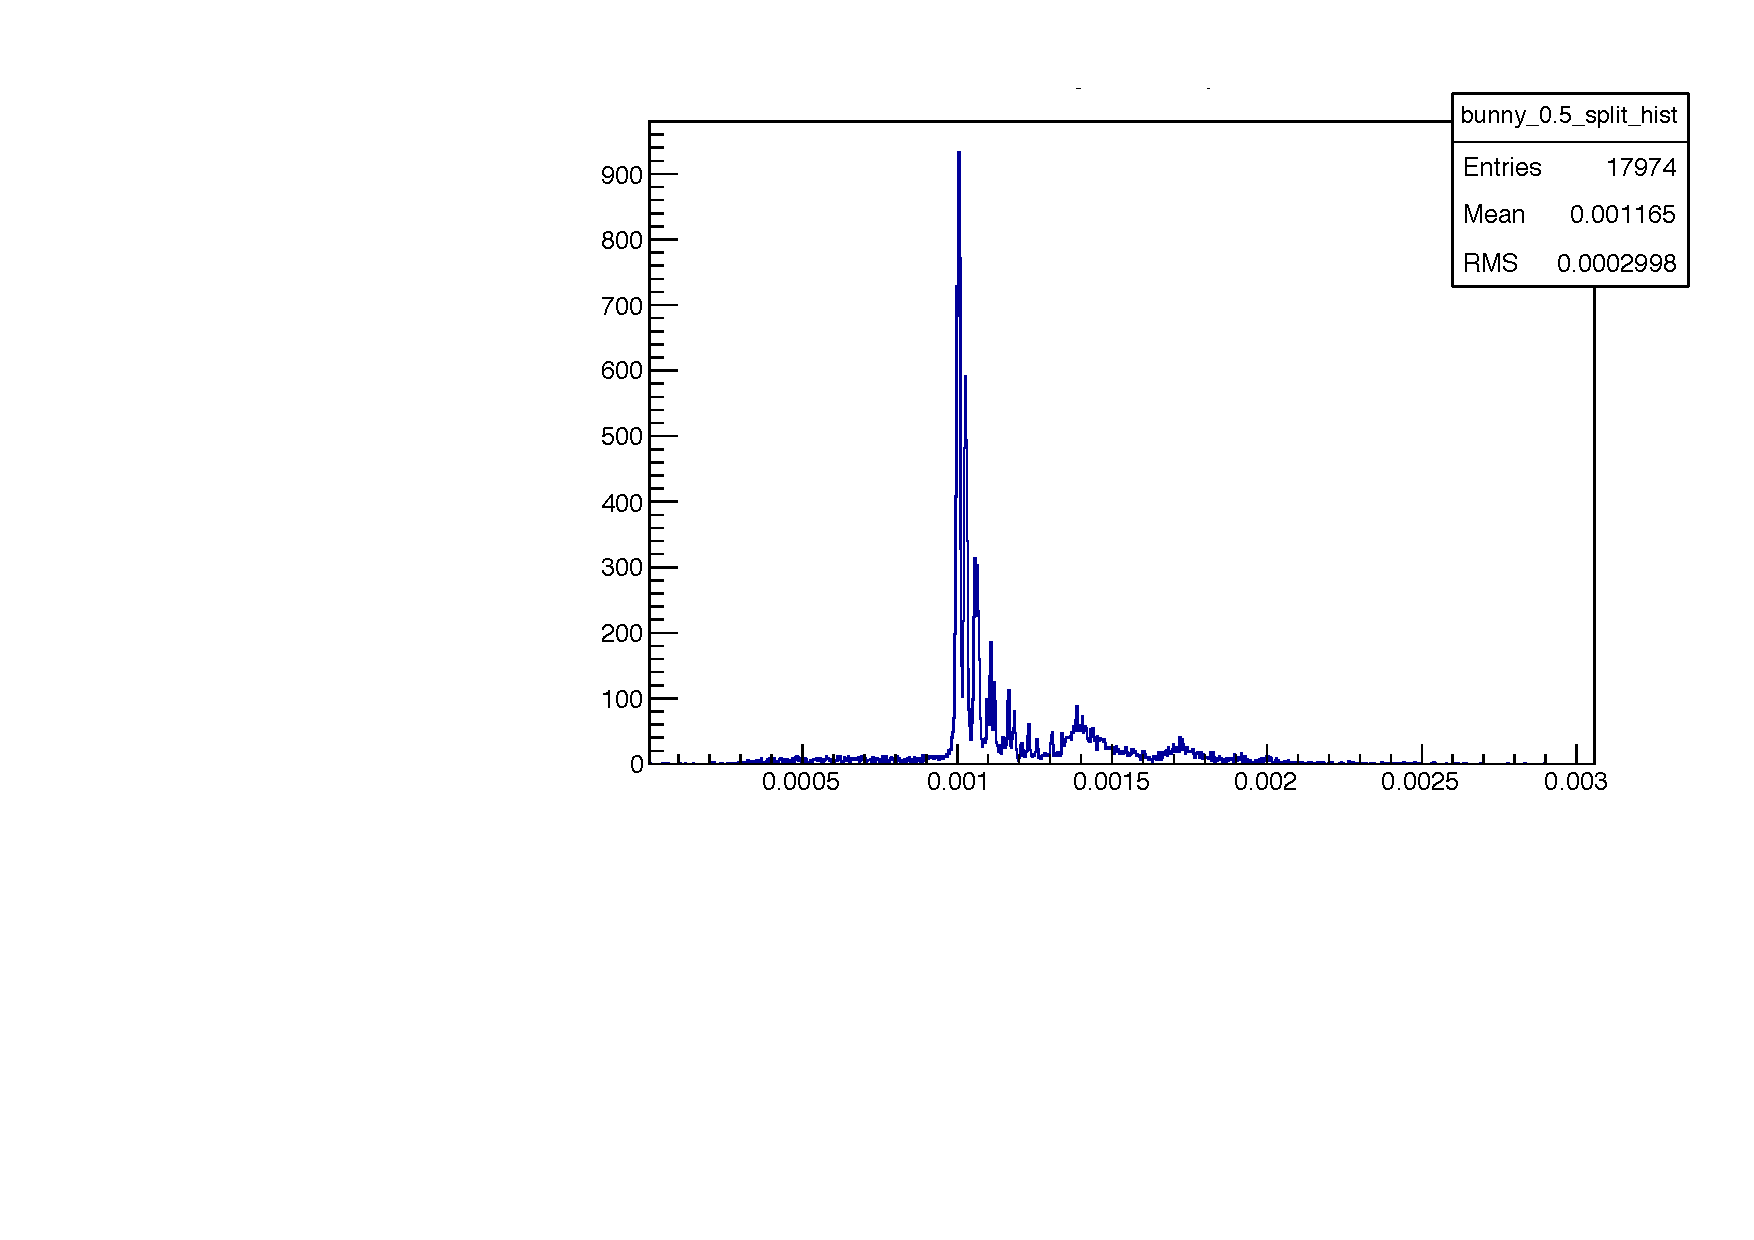
\includegraphics[width=\linewidth]{fig/bunny_05_split.pdf}
\end{subfigure}%
\begin{subfigure}{.5\textwidth}
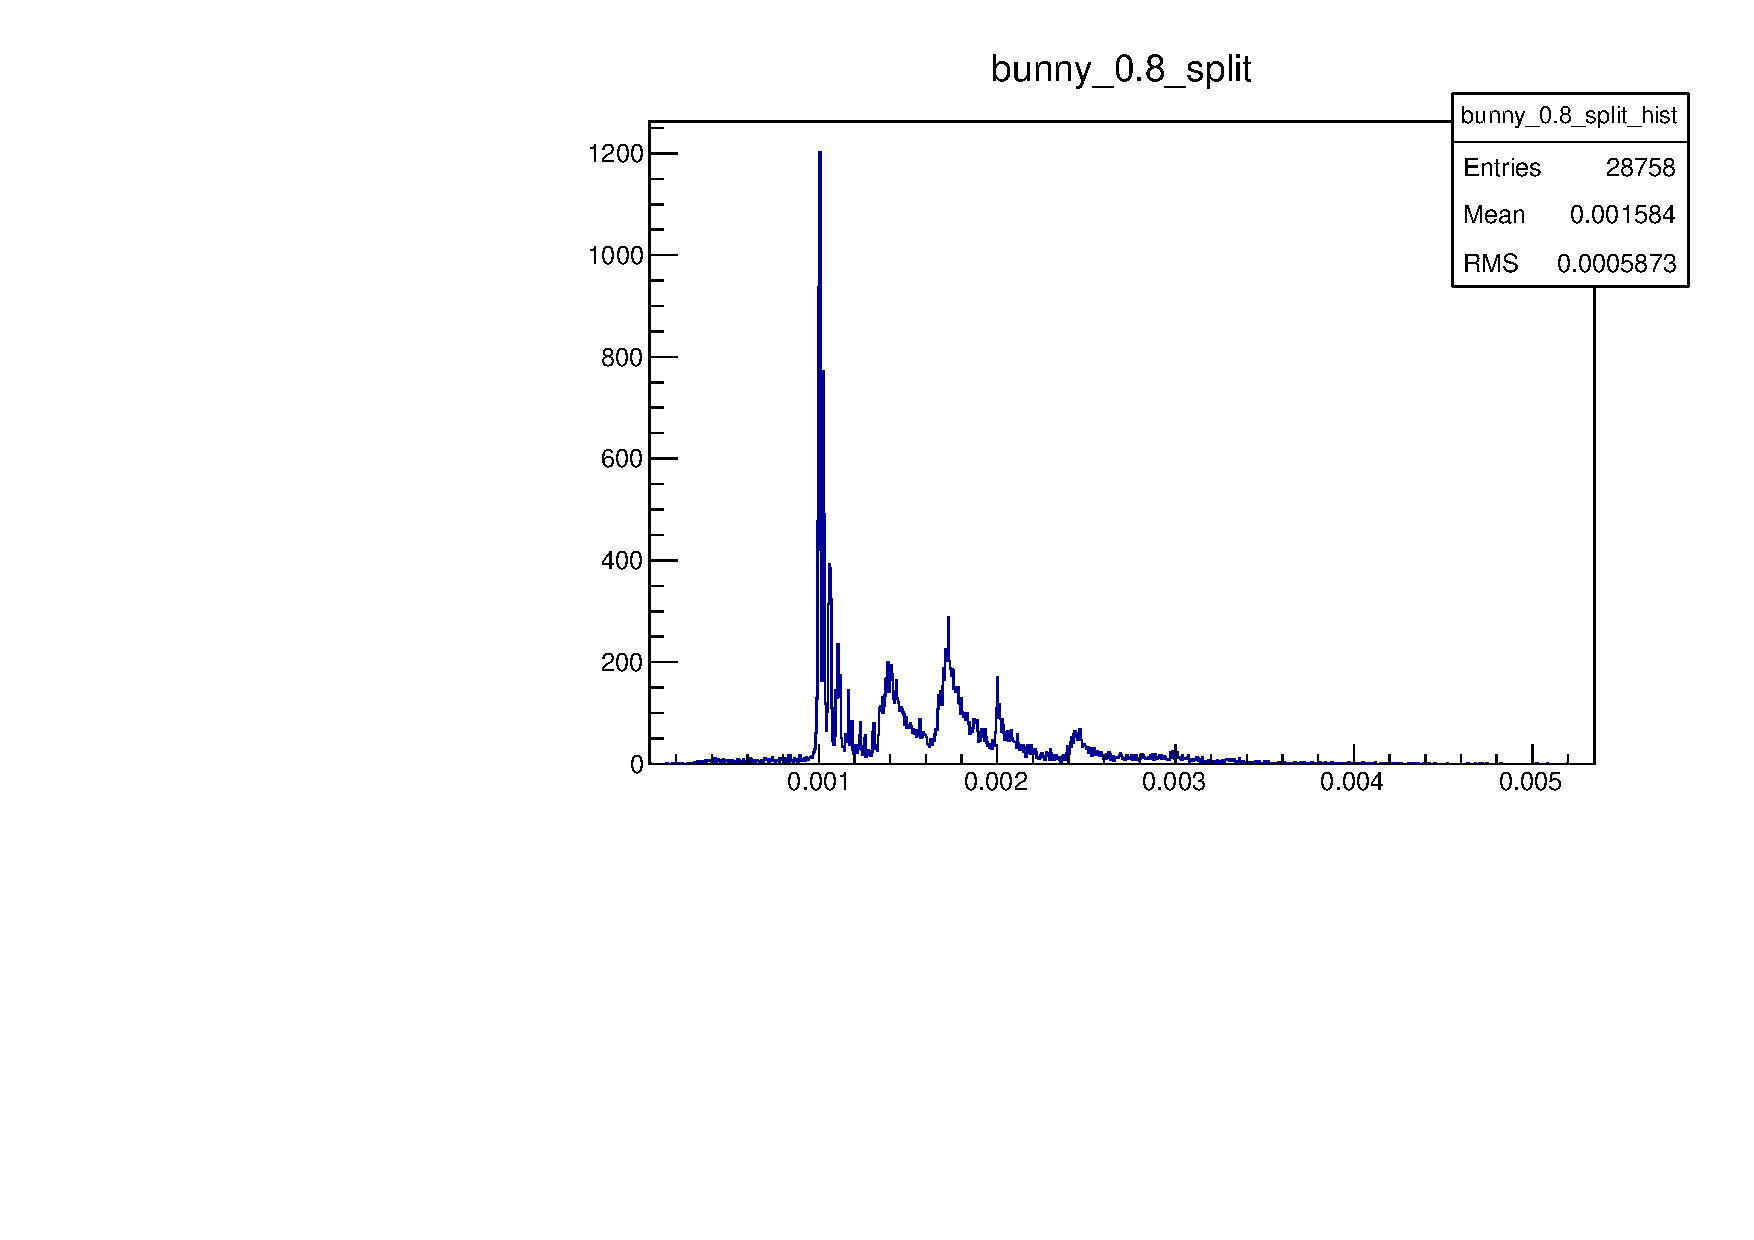
\includegraphics[width=\linewidth]{fig/bunny_08_split.pdf}
\end{subfigure}
\caption{Histograms of $\|q_i - p_i\|$ for 50\% and 80\% split}
\label{fig:bunny_fexp_before}
\end{figure}

In both cases, $\| q - p \| \approx 0.001$ is a mode in the distribution. Smaller values are infrequent. Additional spikes occur for some values above $0.001$. 

The reason is that for the original Bunny point clouds, the points are evenly distributed on the surface on an approximatively square grid, with a mean distance of about $0.001$ between adjacent points, as seen in the close-up view in figure \ref{fig:bunny_grid_closeup}. Figure \ref{fig:bunny_closest} shows a histogram made by taking from each point $p$ on the Bunny point cloud $B$, the closest point $p' \in B$ with $p' \neq p$. In the closest point histograms from $Q$ to $P$, any point that is in $Q$ is missing in $P$ and hence the closest point is often the one at a distance of $0.001$. Some instances appear where this point is not in $P$ either, so the closest point is further. This explains the spike at $0.002$. The other spikes occur when the closest point is in a diagonal direction on the grid. This ``grid'' is approximate and the surface is embedded in a non planar way in 3D space, so most samples do not fall exactly in one of these spikes.

For the true correspondences, the histogram would be a single spike at $\|p_i - q'_i\| = 0$. 



\subsection{Experiments on relief}



\subsection{Limits of accuracy}




\subsection{Metric for resolution}
Informally, the resolution of a point cloud indicates how many samples (i.e. points) of the represented object is contains. For a range image taken by a 3D scanner, the resolution is defined with its width and height, which correspond to the number of measurements taken per scan line and the number of scan lines, for its whole field of view.

The assumption was made that the points in the point cloud lie on a set ensemble of two-dimensional surfaces, which are embedded in three-dimensional space. A points density measure in terms of number of points per unit of volume is thus not meaningful. Instead the \emph{density} of the distribution of points on a surface area if used.




\section{Separation of large scans}

\section{Variable density}

\chapter{Implementation}

\section{Architecture}

\section{Usage of C++}

\section{Optimization}

\section{Visualization}

\section{User interface}

\chapter{Conclusion}


\appendix
\chapter{Experimental Results}

\section{ICP registration}

\subsection{Resolutions and \gls{icp} result, Bunny model} \label{sec:ex_bunny_hilo}
\begin{tabularx}{\textwidth}{|r|X|} \hline
Method & ICP. Select all points, closest point criterion, equal weights, no rejection, point-to-point error metric. \\ \hline
Model & Stanford Bunny model. \\ \hline
Fixed & 50\% of model points, randomly chosen. \\ \hline
Loose & Starting from the other 50\%, randomly downsampled by given amount. $60$ steps. \\ \hline
Displacement & See captions on the figures. \\ \hline
Y Axis & True error, after $40$ iterations. \\\hline
X Axis & Number of points in Loose divided by number of points in Fixed. Lower value means Loose has lover resolution. \\ \hline
\end{tabularx}

\subsubsection{No displacement}
The two point clouds are perfectly aligned to start with.

\begin{figure}[H]
\centering
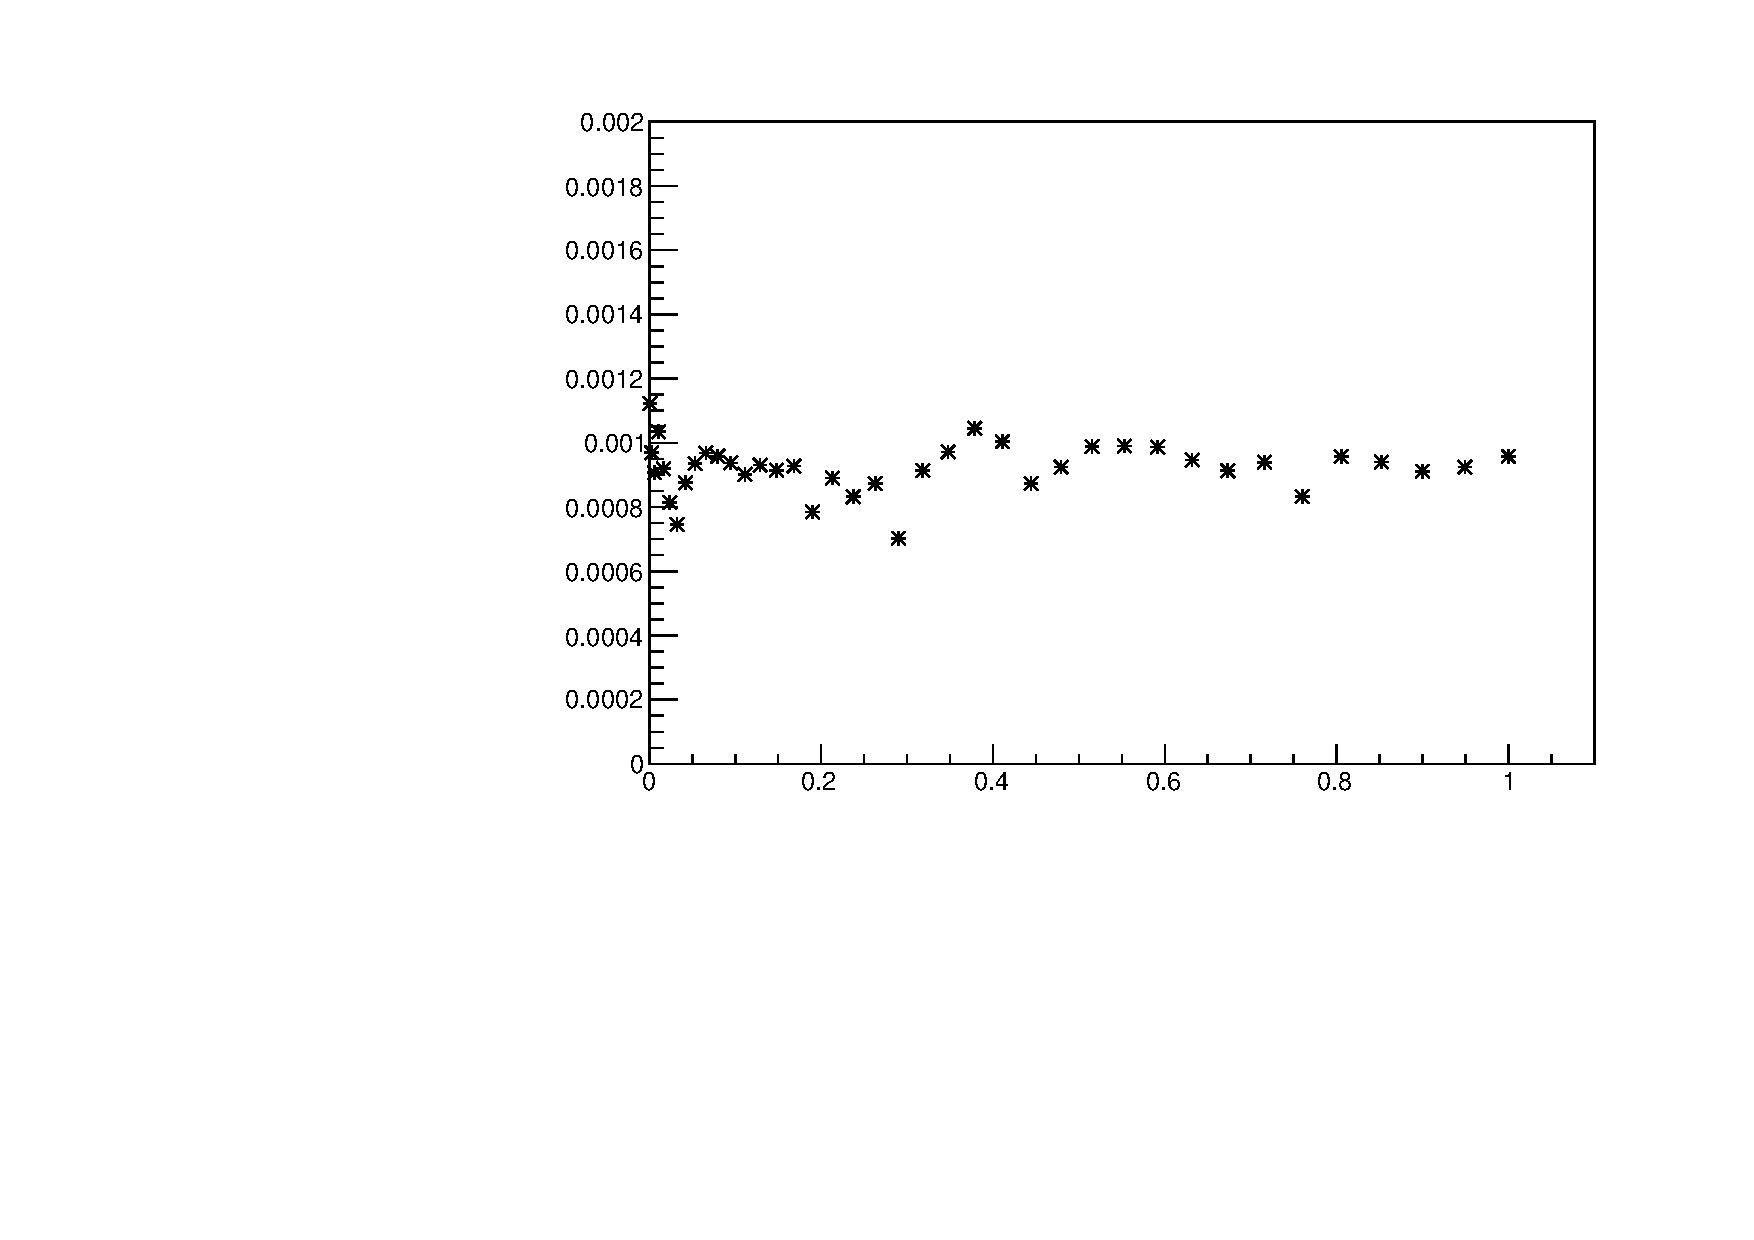
\includegraphics[width=.7\textwidth]{fig/bunny_globmin.pdf}
\caption{no displacement}
\label{fig:bunny_globmin}
\end{figure}

\subsubsection{Small displacement}
Small displacement. Translation by magnitude of $0.01$ in random direction, rotation by $3 \si{\degree}$ or $15 \si{\degree}$ on random axis direction. The Bunny modes has a width, height and depth of about $0.15$.

\begin{figure}[H]
\centering
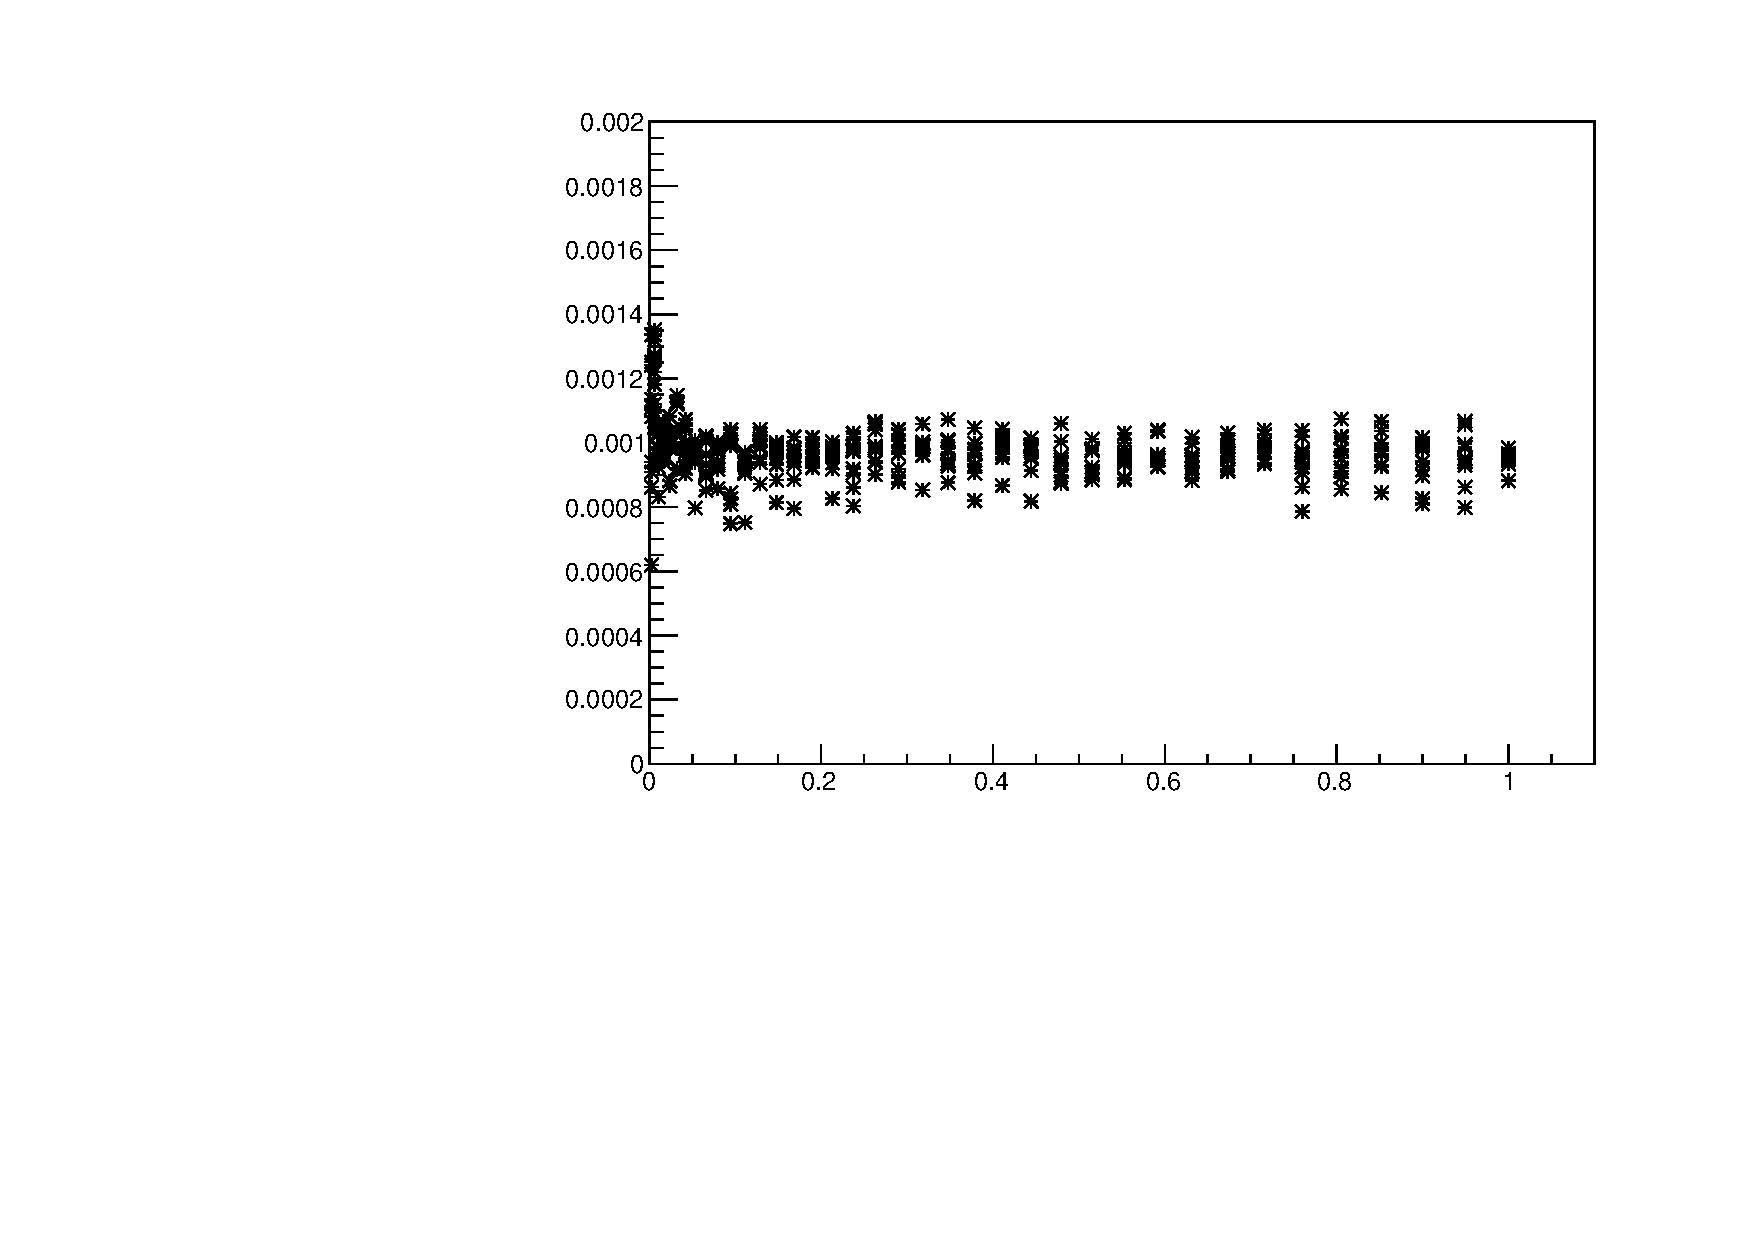
\includegraphics[width=.7\textwidth]{fig/bunny_globsmall.pdf}
\caption{random translation of $0.01$ and rotation of $3 \si{\degree}$, chosen $10$ times}
\label{fig:bunny_globsmall}
\end{figure}

\begin{figure}[H]
\centering
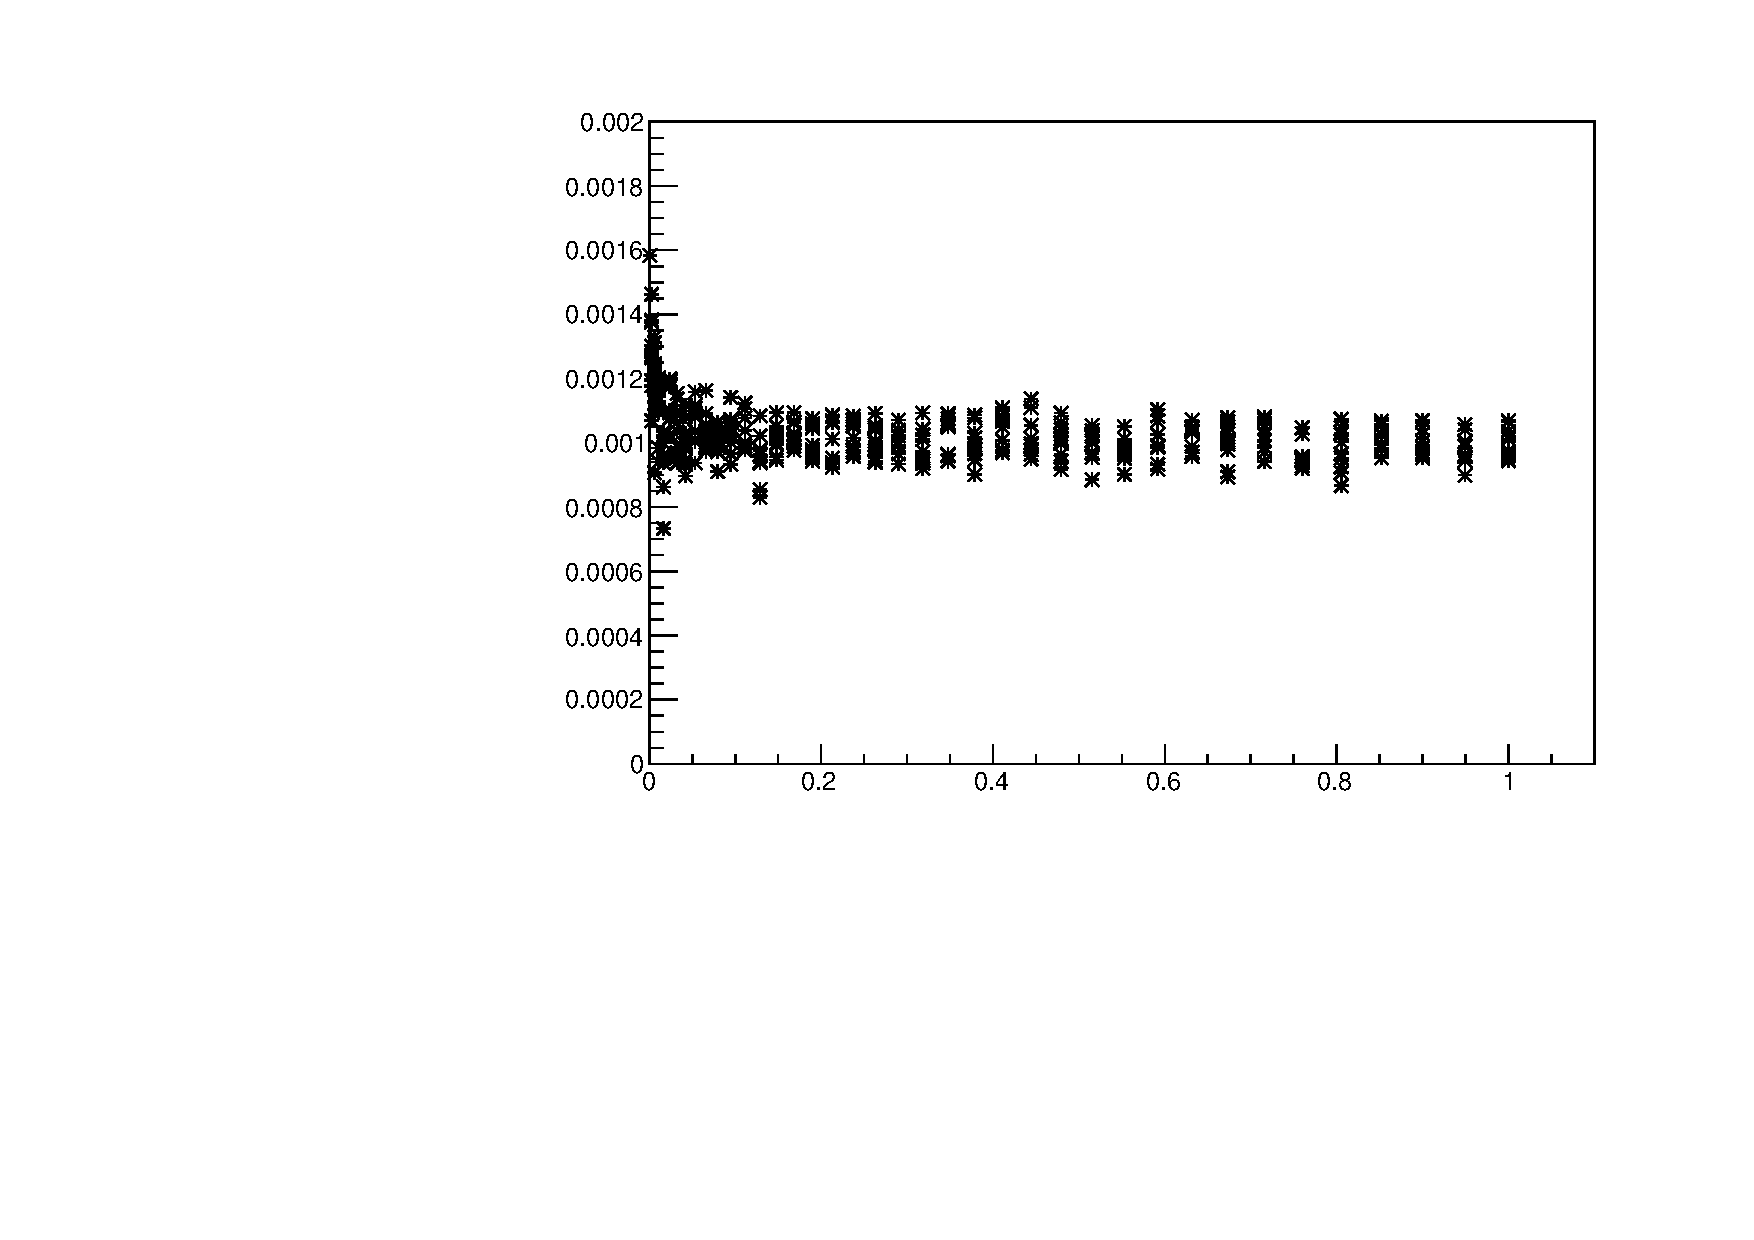
\includegraphics[width=.7\textwidth]{fig/bunny_globmed.pdf}
\caption{random translation of $0.01$ and rotation of $15 \si{\degree}$, chosen $10$ times}
\label{fig:bunny_globmed}
\end{figure}

\subsection{Evolution of \gls{icp} registration, Bunny model}
This plot shows the evolution of the true error \gls{icp} registration, for the same input point clouds. Initially the point clouds are perfectly aligned. The Loose point clouds is randomly generated as before, results from all $60$ registration runs are superimposed.

\begin{tabularx}{\textwidth}{|r|X|} \hline
Method & ICP. Select all points, closest point criterion, equal weights, no rejection, point-to-point error metric. \\ \hline
Model & Stanford Bunny model. \\ \hline
Fixed & 50\% of model points, randomly chosen. \\ \hline
Loose & Starting from the other 50\%, randomly downsampled by given amount. $60$ steps. \\ \hline
Displacement & No displacement. \\ \hline
Y Axis & True error at iteration $i$. \\\hline
X Axis & Iteration step $i$. \\ \hline
\end{tabularx}

\begin{figure}[H]
\centering
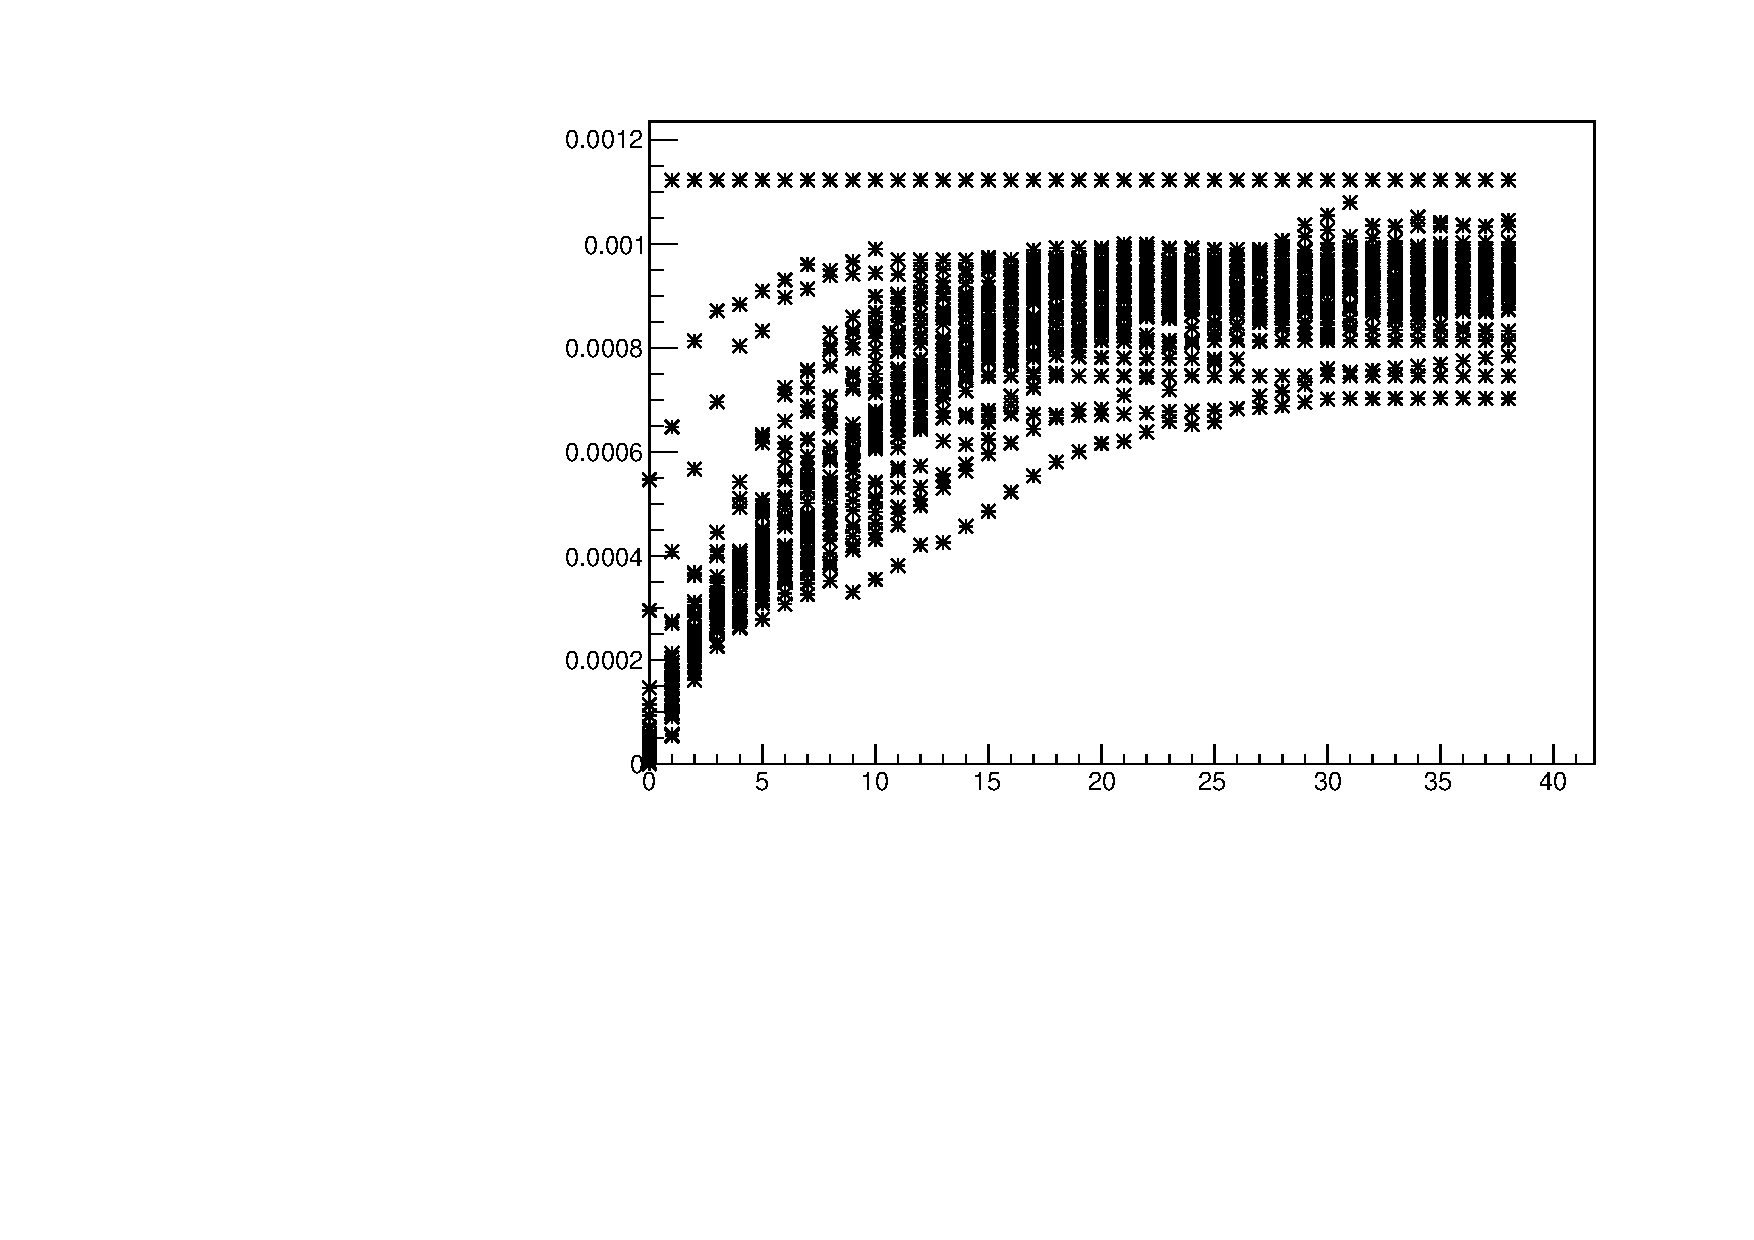
\includegraphics[width=.7\textwidth]{fig/bunny_globmin_ev.pdf}
\caption{Evolutions of true error for experiment \ref{ref:bunny_hilo_a}}
\label{fig:bunny_hilo_ev}
\end{figure}


\subsection{Resolutions and \gls{icp} result, sphere model} \label{sec:ex_sphere_hilo}
\begin{tabularx}{\textwidth}{|r|X|} \hline
Method & ICP. Select all points, closest point criterion, equal weights, no rejection, point-to-point error metric. \\ \hline
Model & Artificially generated sphere point cloud with random point dispersion. \\ \hline
Fixed & Randomly chosen number of points from $0$ to $50000$. $30$ steps. \\ \hline
Loose & Randomly chosen number of points from $0$ to $50000$. $30$ steps. \\ \hline
Displacement & No displacement. \\ \hline
Y Axis & True error, after $40$ iterations. \\\hline
X Axis & Maximum of number of points in Loose and number of points in Fixed. \\ \hline
\end{tabularx}

\begin{figure}[H]
\centering
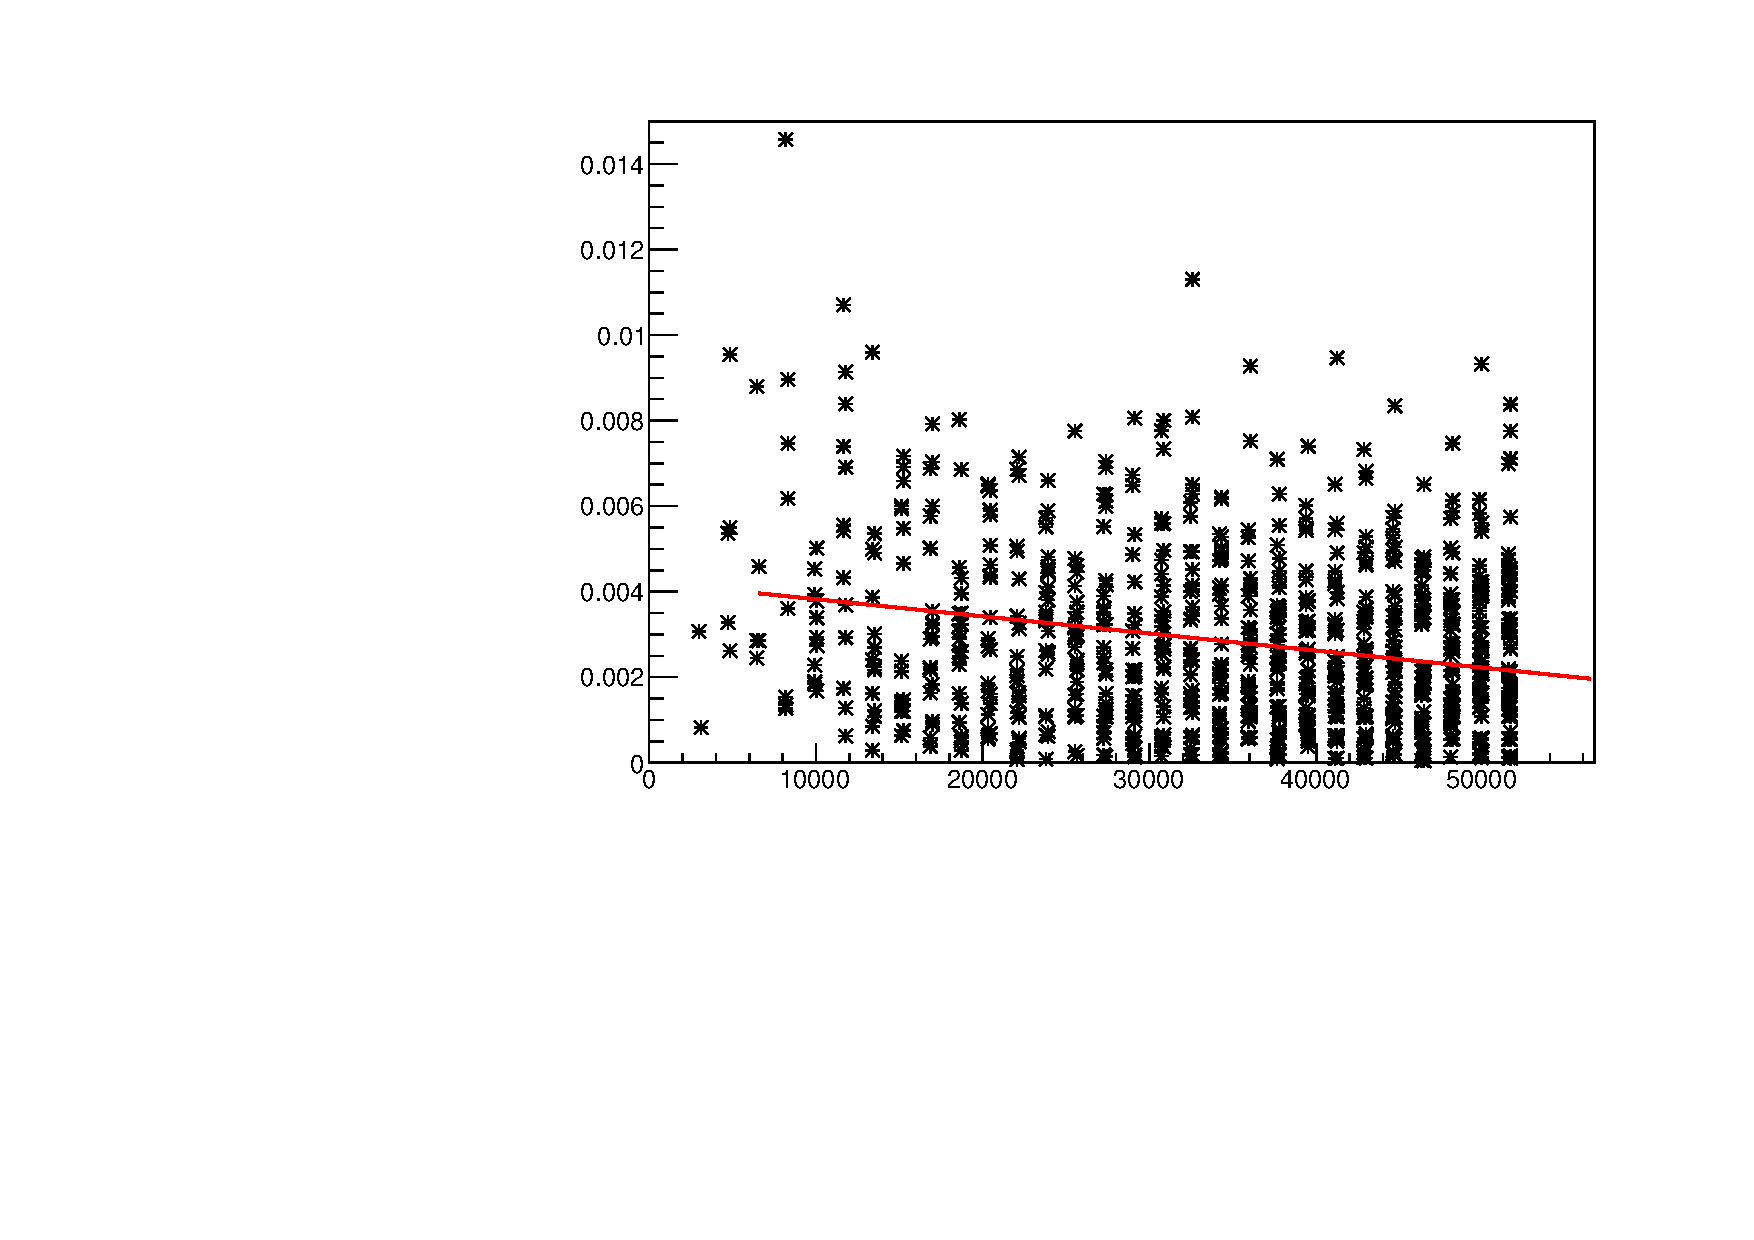
\includegraphics[width=.7\textwidth]{fig/sphere_icp.pdf}
\end{figure}


\subsection{View-point and \gls{icp} result, relief model} \label{sec:ex_relief_dproj}

\begin{tabularx}{\textwidth}{|r|X|} \hline
Method & ICP. Select all points, closest point criterion, equal weights, no rejection, point-to-point error metric. \\ \hline
Model & Relief point cloud, projected with occlusion from camera placed at angle looking down on relief. \\ \hline
Fixed & Point cloud of relief with camera angle varying in $[0, 2 \pi]$ around relief. $20$ steps. \\ \hline
Loose & Point cloud of relief with camera angle varying in $[0, 2 \pi]$ around relief. $20$ steps. \\ \hline
Displacement & No displacement. \\ \hline
Y Axis & True error, after $40$ iterations. \\\hline
X Axis & Angle between Fixed and Loose camera positions. \\ \hline
\end{tabularx}

\begin{figure}[H]
\centering
\includegraphics[width=.7\textwidth]{fig/relief_dproj.pdf}
\end{figure}


\newpage


\section{Relief small transformation \gls{acdh}} \label{sec:relief_small_trans_exp}
The following figures depict \gls{acdh} of a relief point cloud $P$ like the one on figure \ref {fig:relief_plain}, on which a small transformation $\matr{M}$ was applied. For the point cloud $P$, the average nearest neighbor distance on surfaces perpendicular to the camera ray is $p_l = 0.01$. The plane of the relief is along the X and Y axis.

\subsection{Translations}
Translations are applied on two axis, by the amounts \{ 0, 0.002, 0.004, 0.006, 0.008, 0.010 \}.

\subsubsection{X and Y axis} \label{sec:res_acdh_txy}
Here $\matr{M}$ is a translation in X and Y axis, by these amounts. No translation in Z axis and no rotation is applied.

The top-left cell shows the own distance histogram, where $\matr{M} = \matr{I}$. Only translations in the positive directions are made, translations in the negative directions would yield similar results.

\begin{figure}[H]
\foreach \y in {0,1,2,3,4} {
	\foreach \x in {0,1,2,3,4} {
		\includegraphics[width=0.19\linewidth]{fig/cross_relief_trans/(\x-\y-0).pdf}
	}
	\\
}
\caption{Horizontal: X translation, vertical: Y translation}
\end{figure}

\paragraph{Observations}
Translation on the X and on the Y axis have similar results, which is to be expected since the plane of the relief spans in those directions. If $P$ was a perfect plane, the histograms would retain exactly the same shape. Because this is not the case, distances between points on more oblique parts of the surface are increased, resulting in a slightly more convex curvature.

\subsubsection{X and Z axis} \label{sec:res_acdh_txz}
Y axis translation fixed to $0$. Translations by same amounts.

\begin{figure}[H]
\foreach \z in {0,1,2,3,4} {
	\foreach \x in {0,1,2,3,4} {
		\includegraphics[width=0.19\linewidth]{fig/cross_relief_trans/(\x-0-\z).pdf}
	}
	\\
}
\caption{Horizontal: X translation, vertical: Z translation}
\label{fig:ex_trans_xz}
\end{figure}

\paragraph{Observations}
Translation on the X axis is the same as before. But the translation on the Z axis pulls the surfaces, and the histogram gets an offset to the right side. Some oblique surfaces of the model remain close, explaining that parts of the linear increase can remain unchanged.

\newpage


\subsection{Rotations}
Here instead of a translation, a rotation gets applied on the same point cloud. The point of rotation is the center point of the relief plane. The amounts of rotation are \{ 0, 1\si{\degree}, 2\si{\degree}, 3\si{\degree}, 4\si{\degree}, 5\si{\degree} \}.

\subsubsection{Rotation around X and Y axis} \label{sec:res_acdh_rxy}
\begin{figure}[H]
\foreach \y in {0,1,2,3,4} {
	\foreach \x in {0,1,2,3,4} {
		\includegraphics[width=0.19\linewidth]{fig/cross_relief_rot/(\x-\y-0).pdf}
	}
	\\
}
\caption{Horizontal: X axis rotation, vertical: Y axis rotation}
\end{figure}

\paragraph{Observations}
When the point cloud is rotated along the center point, distances of points change more, the further the points are from the center. Because less distances are recorded within the range $[0, \frac{1}{2} l_{\text{min}}]$, the adjusted histogram becomes more jagged.


\subsubsection{Rotation around X and Z axis} \label{sec:res_acdh_rxz}
\begin{figure}[H]
\foreach \z in {0,1,2,3,4} {
	\foreach \x in {0,1,2,3,4} {
		\includegraphics[width=0.19\linewidth]{fig/cross_relief_rot/(\x-0-\z).pdf}
	}
	\\
}
\caption{Horizontal: X axis rotation, vertical: Z axis rotation}
\end{figure}

\paragraph{Observations}
The results are similar as before. The increase in jaggedness is weaker for rotations on the Z axis, because a larger part of the surfaces do not get pulled off each other but slide on each other.



\newpage


\section{Relief small transformation \gls{arcdh}}
Here the same translations are rotations are applied, and the \gls{arcdh} instead of the \gls{acdh} is shown.

\subsection{Translations}

\subsubsection{Translation in X and Y axis} \label{sec:res_arcdh_txy}

\begin{figure}[H]
\foreach \y in {0,1,2,3,4} {
	\foreach \x in {0,1,2,3,4} {
		\includegraphics[width=0.19\linewidth]{fig/cross_relief_trans_rej/(\x-\y-0).pdf}
	}
	\\
}
\caption{Horizontal: X translation, vertical: Y translation}
\end{figure}

\paragraph{Observations}
The histograms remain unchanged. In comparison to \ref{sec:res_acdh_txy}, the effect of the oblique surfaces get cancelled out because points are projected back onto the surface after the translation.

\subsubsection{Translation in X and Z axis} \label{sec:res_arcdh_txz}

\begin{figure}[H]
\foreach \z in {0,1,2,3,4} {
	\foreach \x in {0,1,2,3,4} {
		\includegraphics[width=0.19\linewidth]{fig/cross_relief_trans_rej/(\x-0-\z).pdf}
	}
	\\
}
\caption{Horizontal: X translation, vertical: Z translation}
\label{fig:ex_trans_xz_rej}
\end{figure}

\paragraph{Observations}
The histograms also remain unchanged.

\newpage

\subsection{Rotations}

\subsubsection{Rotation around X and Y axis} \label{sec:res_arcdh_rxy}
\begin{figure}[H]
\foreach \y in {0,1,2,3,4} {
	\foreach \x in {0,1,2,3,4} {
		\includegraphics[width=0.19\linewidth]{fig/cross_relief_rot_rej/(\x-\y-0).pdf}
	}
	\\
}
\caption{Horizontal: X axis rotation, vertical: Y axis rotation}
\end{figure}

\paragraph{Observations} It can be observed that the histogram becomes slightly less linear and more jagged with larger rotation angles.


\subsubsection{Rotation around X and Z axis} \label{sec:res_arcdh_rxz}
\begin{figure}[H]
\foreach \z in {0,1,2,3,4} {
	\foreach \x in {0,1,2,3,4} {
		\includegraphics[width=0.19\linewidth]{fig/cross_relief_rot_rej/(\x-0-\z).pdf}
	}
	\\
}
\caption{Horizontal: X axis rotation, vertical: Z axis rotation}
\end{figure}

\paragraph{Observations} Same as for the rotation on X and Y axis.


\newpage

\section{\Gls{acdh} histogram comparison error metric} \label{sec:chi_err}
For all of these tests, a relief point cloud is used. The plots in the first row show the histogram comparison error metric, while second row shows the mean absolute error with the closest point criterion.

The three columns differ by the range of the transformations applied. The maximal rotation and translations are the following:

\begin{figure}[H]
\centering
\begin{tabularx}{.4\textwidth}{|r|X|X|} \hline
scale  & translation & rotation \\ \hline
L      & 0.1         & 2.29\si{\degree} \\
M      & 0.01        & 0.23\si{\degree} \\
S      & 0.001       & 0.023\si{\degree} \\ \hline
\end{tabularx}
\end{figure}

So the plot for M can seen as a zoomed in version of the tenth of the plot for L, around $x = 0$. Same for S and M. However, on each plot, the curves are different random cross sections. The rotation angles are chosen so that a rotation on the X or Y axis results in an average displacement of true corresponding points by about the same about as the listed translation.

In each of the tests, a loose point cloud $Q$ is registered to a fixed point cloud $P$ of the same model, but with different resolution or view-point. $Q$ is the sample point cloud for the histograms and has a higher resolution. A graphic is shown with each test that shows a close-up view of both point dispersions, along with a scale indicating the L, M and S translation lengths.





\subsection{Same}
Here $Q$ only has a slightly higher resolution to $P$. The close-up view \ref{fig:t_scale} shows the density of $P$ (black) and $Q$ (blue), along with the maximal extent of the translations for the three columns. 

\begin{figure}[h]
\center
{
\setlength{\fboxsep}{0pt}%
\setlength{\fboxrule}{0.5pt}%
\fbox{\includegraphics[width=0.4\textwidth]{fig/t_scale.png}}
}
\label{fig:t_scale}
\caption{Close-up view with scale}
\end{figure}

\begin{figure}[H]
\begin{subfigure}{.33\textwidth}
	\includegraphics[width=\linewidth]{fig/ajherr/t/L_chi.pdf}
\end{subfigure}%
\begin{subfigure}{.33\textwidth}
	\includegraphics[width=\linewidth]{fig/ajherr/t/M_chi.pdf}
\end{subfigure}&
\begin{subfigure}{.33\textwidth}
	\includegraphics[width=\linewidth]{fig/ajherr/t/S_chi.pdf}
\end{subfigure}\\
\begin{subfigure}{.33\textwidth}
	\includegraphics[width=\linewidth]{fig/ajherr/t/L_mae.pdf}
	\caption{L}
\end{subfigure}%
\begin{subfigure}{.33\textwidth}
	\includegraphics[width=\linewidth]{fig/ajherr/t/M_mae.pdf}
	\caption{M}
\end{subfigure}&
\begin{subfigure}{.33\textwidth}
	\includegraphics[width=\linewidth]{fig/ajherr/t/S_mae.pdf}
	\caption{S}
\end{subfigure}\\
\end{figure}

\paragraph{Observations} Firstly, it can be seen that the histogram comparison error metric $e_{\chi}$ is indeed an error metric for the registration. But no improvement compared to the mean absolute error can be seen. For large transformations, $e_{\chi}$ diverges, which is expected because the points $q$ are far away from the parallelogram lattice of $P$, making the histogram comparison results meaningless. For the scale M, the qualities of the error metrics are about the same. On scale $S$, the metric $e_{\chi}$ degenerates, but the mean absolute error remains more stable.


\subsection{Different view-points}
Here the resolutions are the same, but $P$ and $Q$ are projections from different view-points, and the overlap is lower.

\begin{figure}[H]
\begin{subfigure}{.33\textwidth}
	\includegraphics[width=\linewidth]{fig/ajherr/t2/L_chi.pdf}
\end{subfigure}%
\begin{subfigure}{.33\textwidth}
	\includegraphics[width=\linewidth]{fig/ajherr/t2/M_chi.pdf}
\end{subfigure}&
\begin{subfigure}{.33\textwidth}
	\includegraphics[width=\linewidth]{fig/ajherr/t2/S_chi.pdf}
\end{subfigure}\\
\begin{subfigure}{.33\textwidth}
	\includegraphics[width=\linewidth]{fig/ajherr/t2/L_mae.pdf}
	\caption{L}
\end{subfigure}%
\begin{subfigure}{.33\textwidth}
	\includegraphics[width=\linewidth]{fig/ajherr/t2/M_mae.pdf}
	\caption{M}
\end{subfigure}&
\begin{subfigure}{.33\textwidth}
	\includegraphics[width=\linewidth]{fig/ajherr/t2/S_mae.pdf}
	\caption{S}
\end{subfigure}\\
\end{figure}

\paragraph{Observations} The results are similar than before. But on the S scale, both $e_{\chi}$ and the mean absolute error degenerate, as there is a lower number of point correspondences. On this example, $e_{\chi}$ appears to remain slightly more stable.


\FloatBarrier


\subsection{Different resolutions}
Here $P$ has a much lower resolution than $Q$. Again the scale is seen on the close-up view on figure \ref{fig:t3_scale}.

\begin{figure}[h]
\center
{
\setlength{\fboxsep}{0pt}%
\setlength{\fboxrule}{0.5pt}%
\fbox{\includegraphics[width=0.4\textwidth]{fig/t3_scale.png}}
}
\label{fig:t3_scale}
\caption{Close-up view with scale}
\end{figure}


\begin{figure}[H]
\begin{subfigure}{.33\textwidth}
	\includegraphics[width=\linewidth]{fig/ajherr/t3/L_chi.pdf}
\end{subfigure}%
\begin{subfigure}{.33\textwidth}
	\includegraphics[width=\linewidth]{fig/ajherr/t3/M_chi.pdf}
\end{subfigure}&
\begin{subfigure}{.33\textwidth}
	\includegraphics[width=\linewidth]{fig/ajherr/t3/S_chi.pdf}
\end{subfigure}\\
\begin{subfigure}{.33\textwidth}
	\includegraphics[width=\linewidth]{fig/ajherr/t3/L_mae.pdf}
	\caption{L}
\end{subfigure}%
\begin{subfigure}{.33\textwidth}
	\includegraphics[width=\linewidth]{fig/ajherr/t3/M_mae.pdf}
	\caption{M}
\end{subfigure}&
\begin{subfigure}{.33\textwidth}
	\includegraphics[width=\linewidth]{fig/ajherr/t3/S_mae.pdf}
	\caption{S}
\end{subfigure}\\
\end{figure}


\paragraph{Observations} To save time, these plots were recorded less precisely.\footnote{This means that the number of intermediary transformations $\matr{M'}$ at which the two error metrics are evaluated it lower, and there are fewer cross-section curves. The point clouds and their resolutions are the same. The plots are drawn as piecewise linear functions.} The results remain similar to before, no improvement of $e_{\chi}$ compared to the mean absolute error metric can be seen. 


\subsubsection{Translation only}
Here only the translational part of the transformation is applied.

\begin{figure}[H]
\begin{subfigure}{.33\textwidth}
	\includegraphics[width=\linewidth]{fig/ajherr/t3t/L_chi.pdf}
\end{subfigure}%
\begin{subfigure}{.33\textwidth}
	\includegraphics[width=\linewidth]{fig/ajherr/t3t/M_chi.pdf}
\end{subfigure}&
\begin{subfigure}{.33\textwidth}
	\includegraphics[width=\linewidth]{fig/ajherr/t3t/S_chi.pdf}
\end{subfigure}\\
\begin{subfigure}{.33\textwidth}
	\includegraphics[width=\linewidth]{fig/ajherr/t3t/L_mae.pdf}
	\caption{L}
\end{subfigure}%
\begin{subfigure}{.33\textwidth}
	\includegraphics[width=\linewidth]{fig/ajherr/t3t/M_mae.pdf}
	\caption{M}
\end{subfigure}&
\begin{subfigure}{.33\textwidth}
	\includegraphics[width=\linewidth]{fig/ajherr/t3t/S_mae.pdf}
	\caption{S}
\end{subfigure}\\
\end{figure}

\paragraph{Observations} Again, no improvement of $e_{\chi}$ compared to mean absolute error.



\subsubsection{Rotation only}
Now only the rotational part is applied.


\begin{figure}[H]
\begin{subfigure}{.33\textwidth}
	\includegraphics[width=\linewidth]{fig/ajherr/t3r/L_chi.pdf}
\end{subfigure}%
\begin{subfigure}{.33\textwidth}
	\includegraphics[width=\linewidth]{fig/ajherr/t3r/M_chi.pdf}
\end{subfigure}&
\begin{subfigure}{.33\textwidth}
	\includegraphics[width=\linewidth]{fig/ajherr/t3r/S_chi.pdf}
\end{subfigure}\\
\begin{subfigure}{.33\textwidth}
	\includegraphics[width=\linewidth]{fig/ajherr/t3r/L_mae.pdf}
	\caption{L}
\end{subfigure}%
\begin{subfigure}{.33\textwidth}
	\includegraphics[width=\linewidth]{fig/ajherr/t3r/M_mae.pdf}
	\caption{M}
\end{subfigure}&
\begin{subfigure}{.33\textwidth}
	\includegraphics[width=\linewidth]{fig/ajherr/t3r/S_mae.pdf}
	\caption{S}
\end{subfigure}\\
\end{figure}


\paragraph{Observations} Again, no improvement of $e_{\chi}$ compared to mean absolute error.


\newpage

\subsection{Different resolutions, rejection}
Here, the same experiments are before are repeated, but the \gls{arcdh} is recorded, producing the $e_{r,\chi}$ error metric.


\subsubsection{Translation only}
Here only the translational part of the transformation is applied.

\begin{figure}[H]
\begin{subfigure}{.33\textwidth}
	\includegraphics[width=\linewidth]{fig/ajherr/t3tr/L_chi.pdf}
\end{subfigure}%
\begin{subfigure}{.33\textwidth}
	\includegraphics[width=\linewidth]{fig/ajherr/t3tr/M_chi.pdf}
\end{subfigure}&
\begin{subfigure}{.33\textwidth}
	\includegraphics[width=\linewidth]{fig/ajherr/t3tr/S_chi.pdf}
\end{subfigure}\\
\begin{subfigure}{.33\textwidth}
	\includegraphics[width=\linewidth]{fig/ajherr/t3tr/L_mae.pdf}
	\caption{L}
\end{subfigure}%
\begin{subfigure}{.33\textwidth}
	\includegraphics[width=\linewidth]{fig/ajherr/t3tr/M_mae.pdf}
	\caption{M}
\end{subfigure}&
\begin{subfigure}{.33\textwidth}
	\includegraphics[width=\linewidth]{fig/ajherr/t3tr/S_mae.pdf}
	\caption{S}
\end{subfigure}\\
\end{figure}

\paragraph{Observations} Still, no improvement of $e_{r,\chi}$ compared to mean absolute error.



\subsubsection{Rotation only}
Now only the rotational part is applied.


\begin{figure}[H]
\begin{subfigure}{.33\textwidth}
	\includegraphics[width=\linewidth]{fig/ajherr/t3rr/L_chi.pdf}
\end{subfigure}%
\begin{subfigure}{.33\textwidth}
	\includegraphics[width=\linewidth]{fig/ajherr/t3rr/M_chi.pdf}
\end{subfigure}&
\begin{subfigure}{.33\textwidth}
	\includegraphics[width=\linewidth]{fig/ajherr/t3rr/S_chi.pdf}
\end{subfigure}\\
\begin{subfigure}{.33\textwidth}
	\includegraphics[width=\linewidth]{fig/ajherr/t3rr/L_mae.pdf}
	\caption{L}
\end{subfigure}%
\begin{subfigure}{.33\textwidth}
	\includegraphics[width=\linewidth]{fig/ajherr/t3rr/M_mae.pdf}
	\caption{M}
\end{subfigure}&
\begin{subfigure}{.33\textwidth}
	\includegraphics[width=\linewidth]{fig/ajherr/t3rr/S_mae.pdf}
	\caption{S}
\end{subfigure}\\
\end{figure}


\paragraph{Observations} At the L and M scales, no results can be observed. The two metrics at the S scale were recorded with more detail, because some result can be seen here: $e_{r,\chi}$ appears to converge towards a local minimum near the true transformation $\matr{M}$.

Because the curves represent values of the error metrics in cross sections of the rigid transformation space, they necessarily intersect at $x = 0$ which represents the true transformation. What is interesting about $e_{r,\chi}$ is that the curves have an inflection point at $x = 0$. The mean absolute error does not show this property.


\subsubsection{Rotation only, different centers}
To verify this, the following two plots were recorded the same way. The first one is recorded the same way as this last plot of $e_{r,\chi}$ at scale S, and again shows the local minimum at the true transformation $\matr{M}$.

On the second plot, the cross sections in the rigid transformation space were instead chosen to intersect at another random transformation located near the true transformation $\matr{M}$. Here the curves still intersect, but no local minimum can be observed.

This result may have been by chance. However, it shows that the inflection points of the curves are not a side effect of the interpolation in the transformations space at $t = 0$. It is were so, it would also be visible on the second plot.

\begin{figure}[H]
\begin{subfigure}{.49\textwidth}
	\includegraphics[width=\linewidth]{fig/ajherr/t3rr/c1.pdf}
	\caption{Centered on true transformation}
\end{subfigure}%
\begin{subfigure}{.49\textwidth}
	\includegraphics[width=\linewidth]{fig/ajherr/t3rr/c2.pdf}
	\caption{Centered on random transformation}
\end{subfigure}
\end{figure}







\bibliographystyle{authordate1}
\bibliography{../reference/references}

\end{document}